\documentclass[twoside]{book}

% Packages required by doxygen
\usepackage{fixltx2e}
\usepackage{calc}
\usepackage{doxygen}
\usepackage[export]{adjustbox} % also loads graphicx
\usepackage{graphicx}
\usepackage[utf8]{inputenc}
\usepackage{makeidx}
\usepackage{multicol}
\usepackage{multirow}
\PassOptionsToPackage{warn}{textcomp}
\usepackage{textcomp}
\usepackage[nointegrals]{wasysym}
\usepackage[table]{xcolor}

% Font selection
\usepackage[T1]{fontenc}
\usepackage[scaled=.90]{helvet}
\usepackage{courier}
\usepackage{amssymb}
\usepackage{sectsty}
\renewcommand{\familydefault}{\sfdefault}
\allsectionsfont{%
  \fontseries{bc}\selectfont%
  \color{darkgray}%
}
\renewcommand{\DoxyLabelFont}{%
  \fontseries{bc}\selectfont%
  \color{darkgray}%
}
\newcommand{\+}{\discretionary{\mbox{\scriptsize$\hookleftarrow$}}{}{}}

% Page & text layout
\usepackage{geometry}
\geometry{%
  a4paper,%
  top=2.5cm,%
  bottom=2.5cm,%
  left=2.5cm,%
  right=2.5cm%
}
\tolerance=750
\hfuzz=15pt
\hbadness=750
\setlength{\emergencystretch}{15pt}
\setlength{\parindent}{0cm}
\setlength{\parskip}{3ex plus 2ex minus 2ex}
\makeatletter
\renewcommand{\paragraph}{%
  \@startsection{paragraph}{4}{0ex}{-1.0ex}{1.0ex}{%
    \normalfont\normalsize\bfseries\SS@parafont%
  }%
}
\renewcommand{\subparagraph}{%
  \@startsection{subparagraph}{5}{0ex}{-1.0ex}{1.0ex}{%
    \normalfont\normalsize\bfseries\SS@subparafont%
  }%
}
\makeatother

% Headers & footers
\usepackage{fancyhdr}
\pagestyle{fancyplain}
\fancyhead[LE]{\fancyplain{}{\bfseries\thepage}}
\fancyhead[CE]{\fancyplain{}{}}
\fancyhead[RE]{\fancyplain{}{\bfseries\leftmark}}
\fancyhead[LO]{\fancyplain{}{\bfseries\rightmark}}
\fancyhead[CO]{\fancyplain{}{}}
\fancyhead[RO]{\fancyplain{}{\bfseries\thepage}}
\fancyfoot[LE]{\fancyplain{}{}}
\fancyfoot[CE]{\fancyplain{}{}}
\fancyfoot[RE]{\fancyplain{}{\bfseries\scriptsize Generated by Doxygen }}
\fancyfoot[LO]{\fancyplain{}{\bfseries\scriptsize Generated by Doxygen }}
\fancyfoot[CO]{\fancyplain{}{}}
\fancyfoot[RO]{\fancyplain{}{}}
\renewcommand{\footrulewidth}{0.4pt}
\renewcommand{\chaptermark}[1]{%
  \markboth{#1}{}%
}
\renewcommand{\sectionmark}[1]{%
  \markright{\thesection\ #1}%
}

% Indices & bibliography
\usepackage{natbib}
\usepackage[titles]{tocloft}
\setcounter{tocdepth}{3}
\setcounter{secnumdepth}{5}
\makeindex

% Hyperlinks (required, but should be loaded last)
\usepackage{ifpdf}
\ifpdf
  \usepackage[pdftex,pagebackref=true]{hyperref}
\else
  \usepackage[ps2pdf,pagebackref=true]{hyperref}
\fi
\hypersetup{%
  colorlinks=true,%
  linkcolor=blue,%
  citecolor=blue,%
  unicode%
}

% Custom commands
\newcommand{\clearemptydoublepage}{%
  \newpage{\pagestyle{empty}\cleardoublepage}%
}

\usepackage{caption}
\captionsetup{labelsep=space,justification=centering,font={bf},singlelinecheck=off,skip=4pt,position=top}

%===== C O N T E N T S =====

\begin{document}

% Titlepage & ToC
\hypersetup{pageanchor=false,
             bookmarksnumbered=true,
             pdfencoding=unicode
            }
\pagenumbering{roman}
\begin{titlepage}
\vspace*{7cm}
\begin{center}%
{\Large agar.\+io clone }\\
\vspace*{1cm}
{\large Generated by Doxygen 1.8.11}\\
\end{center}
\end{titlepage}
\clearemptydoublepage
\tableofcontents
\clearemptydoublepage
\pagenumbering{arabic}
\hypersetup{pageanchor=true}

%--- Begin generated contents ---
\chapter{Namespace Index}
\section{Namespace List}
Here is a list of all namespaces with brief descriptions\+:\begin{DoxyCompactList}
\item\contentsline{section}{\hyperlink{namespacewebsocket}{websocket} }{\pageref{namespacewebsocket}}{}
\item\contentsline{section}{\hyperlink{namespacewebsocket_1_1http}{websocket\+::http} }{\pageref{namespacewebsocket_1_1http}}{}
\item\contentsline{section}{\hyperlink{namespacewebsocket_1_1http_1_1misc__strings}{websocket\+::http\+::misc\+\_\+strings} }{\pageref{namespacewebsocket_1_1http_1_1misc__strings}}{}
\item\contentsline{section}{\hyperlink{namespacewebsocket_1_1http_1_1status__strings}{websocket\+::http\+::status\+\_\+strings} }{\pageref{namespacewebsocket_1_1http_1_1status__strings}}{}
\end{DoxyCompactList}

\chapter{Hierarchical Index}
\section{Class Hierarchy}
This inheritance list is sorted roughly, but not completely, alphabetically\+:\begin{DoxyCompactList}
\item \contentsline{section}{Element}{\pageref{classElement}}{}
\begin{DoxyCompactList}
\item \contentsline{section}{Ball}{\pageref{classBall}}{}
\item \contentsline{section}{Food\+Item}{\pageref{classFoodItem}}{}
\end{DoxyCompactList}
\item \contentsline{section}{Game\+Board}{\pageref{classGameBoard}}{}
\item \contentsline{section}{Player}{\pageref{classPlayer}}{}
\item \contentsline{section}{Stat}{\pageref{classStat}}{}
\item \contentsline{section}{Update\+Element\+Data}{\pageref{structUpdateElementData}}{}
\item \contentsline{section}{Web\+Server}{\pageref{classWebServer}}{}
\end{DoxyCompactList}

\chapter{Class Index}
\section{Class List}
Here are the classes, structs, unions and interfaces with brief descriptions\+:\begin{DoxyCompactList}
\item\contentsline{section}{\hyperlink{classBall}{Ball} }{\pageref{classBall}}{}
\item\contentsline{section}{\hyperlink{classElement}{Element} }{\pageref{classElement}}{}
\item\contentsline{section}{\hyperlink{classFoodItem}{Food\+Item} }{\pageref{classFoodItem}}{}
\item\contentsline{section}{\hyperlink{classGameBoard}{Game\+Board} }{\pageref{classGameBoard}}{}
\item\contentsline{section}{\hyperlink{classPlayer}{Player} }{\pageref{classPlayer}}{}
\item\contentsline{section}{\hyperlink{classStat}{Stat} }{\pageref{classStat}}{}
\item\contentsline{section}{\hyperlink{structUpdateElementData}{Update\+Element\+Data} }{\pageref{structUpdateElementData}}{}
\item\contentsline{section}{\hyperlink{classWebServer}{Web\+Server} }{\pageref{classWebServer}}{}
\end{DoxyCompactList}

\chapter{File Index}
\section{File List}
Here is a list of all documented files with brief descriptions\+:\begin{DoxyCompactList}
\item\contentsline{section}{{\bfseries ball.\+hpp} }{\pageref{ball_8hpp}}{}
\item\contentsline{section}{{\bfseries element.\+hpp} }{\pageref{element_8hpp}}{}
\item\contentsline{section}{{\bfseries food\+Item.\+hpp} }{\pageref{foodItem_8hpp}}{}
\item\contentsline{section}{{\bfseries game\+Board.\+hpp} }{\pageref{gameBoard_8hpp}}{}
\item\contentsline{section}{\hyperlink{main_8cpp}{main.\+cpp} }{\pageref{main_8cpp}}{}
\item\contentsline{section}{{\bfseries player.\+hpp} }{\pageref{player_8hpp}}{}
\item\contentsline{section}{{\bfseries stat.\+hpp} }{\pageref{stat_8hpp}}{}
\item\contentsline{section}{{\bfseries webserver.\+hpp} }{\pageref{webserver_8hpp}}{}
\end{DoxyCompactList}

\chapter{Namespace Documentation}
\hypertarget{namespacewebsocket}{}\section{websocket Namespace Reference}
\label{namespacewebsocket}\index{websocket@{websocket}}
\subsection*{Namespaces}
\begin{DoxyCompactItemize}
\item 
 \hyperlink{namespacewebsocket_1_1http}{http}
\end{DoxyCompactItemize}
\subsection*{Classes}
\begin{DoxyCompactItemize}
\item 
class \hyperlink{classwebsocket_1_1Ball}{Ball}
\item 
struct \hyperlink{structwebsocket_1_1Dataframe}{Dataframe}
\item 
class \hyperlink{classwebsocket_1_1DataframeParser}{Dataframe\+Parser}
\item 
class \hyperlink{classwebsocket_1_1Element}{Element}
\item 
class \hyperlink{classwebsocket_1_1FoodItem}{Food\+Item}
\item 
class \hyperlink{classwebsocket_1_1GameBoard}{Game\+Board}
\item 
class \hyperlink{classwebsocket_1_1Player}{Player}
\item 
class \hyperlink{classwebsocket_1_1Server}{Server}
\item 
class \hyperlink{classwebsocket_1_1Session}{Session}
\end{DoxyCompactItemize}
\subsection*{Typedefs}
\begin{DoxyCompactItemize}
\item 
typedef std\+::shared\+\_\+ptr$<$ \hyperlink{classwebsocket_1_1Ball}{Ball} $>$ \hyperlink{namespacewebsocket_aae1d9cf317a0fb0b83bdfc2f92df77c7}{ball\+\_\+ptr}
\item 
typedef std\+::shared\+\_\+ptr$<$ \hyperlink{classwebsocket_1_1Element}{Element} $>$ \hyperlink{namespacewebsocket_a1f36ba91b301b228fa9e9f812883050c}{element\+\_\+ptr}
\item 
typedef std\+::shared\+\_\+ptr$<$ \hyperlink{classwebsocket_1_1FoodItem}{Food\+Item} $>$ \hyperlink{namespacewebsocket_a198017789b8c5fa32315a12d5ce97869}{food\+\_\+ptr}
\item 
typedef std\+::deque$<$ \hyperlink{structwebsocket_1_1Dataframe}{Dataframe} $>$ \hyperlink{namespacewebsocket_ae3fdf29bb367b5baf5be703253a4edfa}{message\+\_\+queue}
\item 
typedef boost\+::shared\+\_\+ptr$<$ \hyperlink{classwebsocket_1_1Player}{Player} $>$ \hyperlink{namespacewebsocket_aec8d52893bdf524a1412533a63b006a3}{player\+\_\+ptr}
\item 
typedef boost\+::shared\+\_\+ptr$<$ \hyperlink{classwebsocket_1_1Session}{Session} $>$ \hyperlink{namespacewebsocket_a12d8500a66e77dc9bfbff046b86714d8}{session\+\_\+ptr}
\end{DoxyCompactItemize}


\subsection{Typedef Documentation}
\index{websocket@{websocket}!ball\+\_\+ptr@{ball\+\_\+ptr}}
\index{ball\+\_\+ptr@{ball\+\_\+ptr}!websocket@{websocket}}
\subsubsection[{\texorpdfstring{ball\+\_\+ptr}{ball_ptr}}]{\setlength{\rightskip}{0pt plus 5cm}typedef std\+::shared\+\_\+ptr$<${\bf Ball}$>$ {\bf websocket\+::ball\+\_\+ptr}}\hypertarget{namespacewebsocket_aae1d9cf317a0fb0b83bdfc2f92df77c7}{}\label{namespacewebsocket_aae1d9cf317a0fb0b83bdfc2f92df77c7}
\index{websocket@{websocket}!element\+\_\+ptr@{element\+\_\+ptr}}
\index{element\+\_\+ptr@{element\+\_\+ptr}!websocket@{websocket}}
\subsubsection[{\texorpdfstring{element\+\_\+ptr}{element_ptr}}]{\setlength{\rightskip}{0pt plus 5cm}typedef std\+::shared\+\_\+ptr$<${\bf Element}$>$ {\bf websocket\+::element\+\_\+ptr}}\hypertarget{namespacewebsocket_a1f36ba91b301b228fa9e9f812883050c}{}\label{namespacewebsocket_a1f36ba91b301b228fa9e9f812883050c}
\index{websocket@{websocket}!food\+\_\+ptr@{food\+\_\+ptr}}
\index{food\+\_\+ptr@{food\+\_\+ptr}!websocket@{websocket}}
\subsubsection[{\texorpdfstring{food\+\_\+ptr}{food_ptr}}]{\setlength{\rightskip}{0pt plus 5cm}typedef std\+::shared\+\_\+ptr$<${\bf Food\+Item}$>$ {\bf websocket\+::food\+\_\+ptr}}\hypertarget{namespacewebsocket_a198017789b8c5fa32315a12d5ce97869}{}\label{namespacewebsocket_a198017789b8c5fa32315a12d5ce97869}
\index{websocket@{websocket}!message\+\_\+queue@{message\+\_\+queue}}
\index{message\+\_\+queue@{message\+\_\+queue}!websocket@{websocket}}
\subsubsection[{\texorpdfstring{message\+\_\+queue}{message_queue}}]{\setlength{\rightskip}{0pt plus 5cm}typedef std\+::deque$<${\bf Dataframe}$>$ {\bf websocket\+::message\+\_\+queue}}\hypertarget{namespacewebsocket_ae3fdf29bb367b5baf5be703253a4edfa}{}\label{namespacewebsocket_ae3fdf29bb367b5baf5be703253a4edfa}
\index{websocket@{websocket}!player\+\_\+ptr@{player\+\_\+ptr}}
\index{player\+\_\+ptr@{player\+\_\+ptr}!websocket@{websocket}}
\subsubsection[{\texorpdfstring{player\+\_\+ptr}{player_ptr}}]{\setlength{\rightskip}{0pt plus 5cm}typedef boost\+::shared\+\_\+ptr$<${\bf Player}$>$ {\bf websocket\+::player\+\_\+ptr}}\hypertarget{namespacewebsocket_aec8d52893bdf524a1412533a63b006a3}{}\label{namespacewebsocket_aec8d52893bdf524a1412533a63b006a3}
\index{websocket@{websocket}!session\+\_\+ptr@{session\+\_\+ptr}}
\index{session\+\_\+ptr@{session\+\_\+ptr}!websocket@{websocket}}
\subsubsection[{\texorpdfstring{session\+\_\+ptr}{session_ptr}}]{\setlength{\rightskip}{0pt plus 5cm}typedef boost\+::shared\+\_\+ptr$<${\bf Session}$>$ {\bf websocket\+::session\+\_\+ptr}}\hypertarget{namespacewebsocket_a12d8500a66e77dc9bfbff046b86714d8}{}\label{namespacewebsocket_a12d8500a66e77dc9bfbff046b86714d8}

\hypertarget{namespacewebsocket_1_1http}{}\section{websocket\+:\+:http Namespace Reference}
\label{namespacewebsocket_1_1http}\index{websocket\+::http@{websocket\+::http}}
\subsection*{Namespaces}
\begin{DoxyCompactItemize}
\item 
 \hyperlink{namespacewebsocket_1_1http_1_1misc__strings}{misc\+\_\+strings}
\item 
 \hyperlink{namespacewebsocket_1_1http_1_1status__strings}{status\+\_\+strings}
\end{DoxyCompactItemize}
\subsection*{Classes}
\begin{DoxyCompactItemize}
\item 
struct \hyperlink{structwebsocket_1_1http_1_1Header}{Header}
\item 
struct \hyperlink{structwebsocket_1_1http_1_1Reply}{Reply}
\item 
struct \hyperlink{structwebsocket_1_1http_1_1Request}{Request}
\item 
class \hyperlink{classwebsocket_1_1http_1_1RequestHandler}{Request\+Handler}
\item 
class \hyperlink{classwebsocket_1_1http_1_1RequestParser}{Request\+Parser}
\end{DoxyCompactItemize}

\hypertarget{namespacewebsocket_1_1http_1_1misc__strings}{}\section{websocket\+:\+:http\+:\+:misc\+\_\+strings Namespace Reference}
\label{namespacewebsocket_1_1http_1_1misc__strings}\index{websocket\+::http\+::misc\+\_\+strings@{websocket\+::http\+::misc\+\_\+strings}}
\subsection*{Variables}
\begin{DoxyCompactItemize}
\item 
const char \hyperlink{namespacewebsocket_1_1http_1_1misc__strings_a8fede78f1be63335d445aabd0277727e}{name\+\_\+value\+\_\+separator} \mbox{[}$\,$\mbox{]} = \{ \textquotesingle{}\+:\textquotesingle{}, \textquotesingle{} \textquotesingle{} \}
\item 
const char \hyperlink{namespacewebsocket_1_1http_1_1misc__strings_a570bafe7096a0c7904f41f8d6ada54af}{crlf} \mbox{[}$\,$\mbox{]} = \{ \textquotesingle{}\textbackslash{}r\textquotesingle{}, \textquotesingle{}\textbackslash{}n\textquotesingle{} \}
\end{DoxyCompactItemize}


\subsection{Variable Documentation}
\index{websocket\+::http\+::misc\+\_\+strings@{websocket\+::http\+::misc\+\_\+strings}!crlf@{crlf}}
\index{crlf@{crlf}!websocket\+::http\+::misc\+\_\+strings@{websocket\+::http\+::misc\+\_\+strings}}
\subsubsection[{\texorpdfstring{crlf}{crlf}}]{\setlength{\rightskip}{0pt plus 5cm}const char websocket\+::http\+::misc\+\_\+strings\+::crlf\mbox{[}$\,$\mbox{]} = \{ \textquotesingle{}\textbackslash{}r\textquotesingle{}, \textquotesingle{}\textbackslash{}n\textquotesingle{} \}}\hypertarget{namespacewebsocket_1_1http_1_1misc__strings_a570bafe7096a0c7904f41f8d6ada54af}{}\label{namespacewebsocket_1_1http_1_1misc__strings_a570bafe7096a0c7904f41f8d6ada54af}
\index{websocket\+::http\+::misc\+\_\+strings@{websocket\+::http\+::misc\+\_\+strings}!name\+\_\+value\+\_\+separator@{name\+\_\+value\+\_\+separator}}
\index{name\+\_\+value\+\_\+separator@{name\+\_\+value\+\_\+separator}!websocket\+::http\+::misc\+\_\+strings@{websocket\+::http\+::misc\+\_\+strings}}
\subsubsection[{\texorpdfstring{name\+\_\+value\+\_\+separator}{name_value_separator}}]{\setlength{\rightskip}{0pt plus 5cm}const char websocket\+::http\+::misc\+\_\+strings\+::name\+\_\+value\+\_\+separator\mbox{[}$\,$\mbox{]} = \{ \textquotesingle{}\+:\textquotesingle{}, \textquotesingle{} \textquotesingle{} \}}\hypertarget{namespacewebsocket_1_1http_1_1misc__strings_a8fede78f1be63335d445aabd0277727e}{}\label{namespacewebsocket_1_1http_1_1misc__strings_a8fede78f1be63335d445aabd0277727e}

\hypertarget{namespacewebsocket_1_1http_1_1status__strings}{}\section{websocket\+:\+:http\+:\+:status\+\_\+strings Namespace Reference}
\label{namespacewebsocket_1_1http_1_1status__strings}\index{websocket\+::http\+::status\+\_\+strings@{websocket\+::http\+::status\+\_\+strings}}
\subsection*{Functions}
\begin{DoxyCompactItemize}
\item 
boost\+::asio\+::const\+\_\+buffer \hyperlink{namespacewebsocket_1_1http_1_1status__strings_a71a3c805bd5bbbf577264ca762da4299}{to\+\_\+buffer} (\hyperlink{structwebsocket_1_1http_1_1Reply_ab5757d7340f55ea26952d8a4b26ecff2}{Reply\+::status\+\_\+type} status)
\end{DoxyCompactItemize}
\subsection*{Variables}
\begin{DoxyCompactItemize}
\item 
const std\+::string \hyperlink{namespacewebsocket_1_1http_1_1status__strings_a9b60f1719697fb464b7063cb436e1d75}{switching\+\_\+protocols}
\item 
const std\+::string \hyperlink{namespacewebsocket_1_1http_1_1status__strings_a29073784a5e6444e93b0925153605222}{bad\+\_\+request}
\item 
const std\+::string \hyperlink{namespacewebsocket_1_1http_1_1status__strings_a364b430d5e52bc7600da0bcc5dc0d5fc}{internal\+\_\+server\+\_\+error}
\end{DoxyCompactItemize}


\subsection{Function Documentation}
\index{websocket\+::http\+::status\+\_\+strings@{websocket\+::http\+::status\+\_\+strings}!to\+\_\+buffer@{to\+\_\+buffer}}
\index{to\+\_\+buffer@{to\+\_\+buffer}!websocket\+::http\+::status\+\_\+strings@{websocket\+::http\+::status\+\_\+strings}}
\subsubsection[{\texorpdfstring{to\+\_\+buffer(\+Reply\+::status\+\_\+type status)}{to_buffer(Reply::status_type status)}}]{\setlength{\rightskip}{0pt plus 5cm}boost\+::asio\+::const\+\_\+buffer websocket\+::http\+::status\+\_\+strings\+::to\+\_\+buffer (
\begin{DoxyParamCaption}
\item[{{\bf Reply\+::status\+\_\+type}}]{status}
\end{DoxyParamCaption}
)}\hypertarget{namespacewebsocket_1_1http_1_1status__strings_a71a3c805bd5bbbf577264ca762da4299}{}\label{namespacewebsocket_1_1http_1_1status__strings_a71a3c805bd5bbbf577264ca762da4299}


\subsection{Variable Documentation}
\index{websocket\+::http\+::status\+\_\+strings@{websocket\+::http\+::status\+\_\+strings}!bad\+\_\+request@{bad\+\_\+request}}
\index{bad\+\_\+request@{bad\+\_\+request}!websocket\+::http\+::status\+\_\+strings@{websocket\+::http\+::status\+\_\+strings}}
\subsubsection[{\texorpdfstring{bad\+\_\+request}{bad_request}}]{\setlength{\rightskip}{0pt plus 5cm}const std\+::string websocket\+::http\+::status\+\_\+strings\+::bad\+\_\+request}\hypertarget{namespacewebsocket_1_1http_1_1status__strings_a29073784a5e6444e93b0925153605222}{}\label{namespacewebsocket_1_1http_1_1status__strings_a29073784a5e6444e93b0925153605222}
{\bfseries Initial value\+:}
\begin{DoxyCode}
=
                \textcolor{stringliteral}{"HTTP/1.1 400 Bad Request\(\backslash\)r\(\backslash\)n"}
\end{DoxyCode}
\index{websocket\+::http\+::status\+\_\+strings@{websocket\+::http\+::status\+\_\+strings}!internal\+\_\+server\+\_\+error@{internal\+\_\+server\+\_\+error}}
\index{internal\+\_\+server\+\_\+error@{internal\+\_\+server\+\_\+error}!websocket\+::http\+::status\+\_\+strings@{websocket\+::http\+::status\+\_\+strings}}
\subsubsection[{\texorpdfstring{internal\+\_\+server\+\_\+error}{internal_server_error}}]{\setlength{\rightskip}{0pt plus 5cm}const std\+::string websocket\+::http\+::status\+\_\+strings\+::internal\+\_\+server\+\_\+error}\hypertarget{namespacewebsocket_1_1http_1_1status__strings_a364b430d5e52bc7600da0bcc5dc0d5fc}{}\label{namespacewebsocket_1_1http_1_1status__strings_a364b430d5e52bc7600da0bcc5dc0d5fc}
{\bfseries Initial value\+:}
\begin{DoxyCode}
=
                \textcolor{stringliteral}{"HTTP/1.1 500 Internal Server Error\(\backslash\)r\(\backslash\)n"}
\end{DoxyCode}
\index{websocket\+::http\+::status\+\_\+strings@{websocket\+::http\+::status\+\_\+strings}!switching\+\_\+protocols@{switching\+\_\+protocols}}
\index{switching\+\_\+protocols@{switching\+\_\+protocols}!websocket\+::http\+::status\+\_\+strings@{websocket\+::http\+::status\+\_\+strings}}
\subsubsection[{\texorpdfstring{switching\+\_\+protocols}{switching_protocols}}]{\setlength{\rightskip}{0pt plus 5cm}const std\+::string websocket\+::http\+::status\+\_\+strings\+::switching\+\_\+protocols}\hypertarget{namespacewebsocket_1_1http_1_1status__strings_a9b60f1719697fb464b7063cb436e1d75}{}\label{namespacewebsocket_1_1http_1_1status__strings_a9b60f1719697fb464b7063cb436e1d75}
{\bfseries Initial value\+:}
\begin{DoxyCode}
=
                \textcolor{stringliteral}{"HTTP/1.1 101 Switching Protocols\(\backslash\)r\(\backslash\)n"}
\end{DoxyCode}

\chapter{Class Documentation}
\hypertarget{classwebsocket_1_1Ball}{}\section{websocket\+:\+:Ball Class Reference}
\label{classwebsocket_1_1Ball}\index{websocket\+::\+Ball@{websocket\+::\+Ball}}


{\ttfamily \#include $<$ball.\+hpp$>$}



Inheritance diagram for websocket\+:\+:Ball\+:
\nopagebreak
\begin{figure}[H]
\begin{center}
\leavevmode
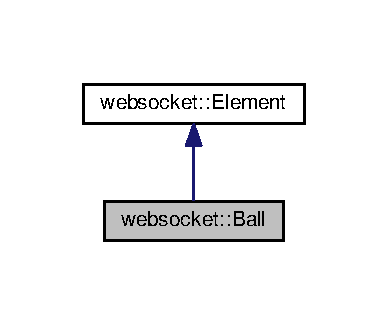
\includegraphics[width=186pt]{classwebsocket_1_1Ball__inherit__graph}
\end{center}
\end{figure}


Collaboration diagram for websocket\+:\+:Ball\+:
\nopagebreak
\begin{figure}[H]
\begin{center}
\leavevmode
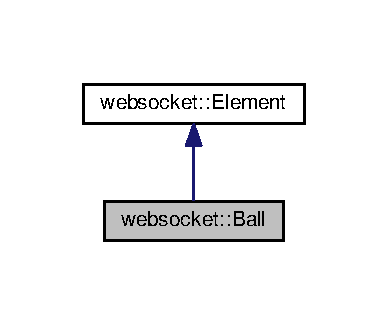
\includegraphics[width=186pt]{classwebsocket_1_1Ball__coll__graph}
\end{center}
\end{figure}
\subsection*{Public Member Functions}
\begin{DoxyCompactItemize}
\item 
\hyperlink{classwebsocket_1_1Ball_a1d933b1f878ee0bcd00e2db1b10c44c2}{Ball} (double \&x, double \&y, double \&radius)
\item 
virtual \hyperlink{classwebsocket_1_1Ball_a07e8b6854de320eeb0def600daece544}{$\sim$\+Ball} ()
\item 
\hyperlink{classwebsocket_1_1Ball_a0b3751d6c313f7bda53eb409196f7c9d}{Ball} (const \hyperlink{classwebsocket_1_1Ball}{Ball} \&other)=default
\item 
\hyperlink{classwebsocket_1_1Ball}{Ball} \& \hyperlink{classwebsocket_1_1Ball_abd82c6929644366316b7ea7b0c14e186}{operator=} (const \hyperlink{classwebsocket_1_1Ball}{Ball} \&other)=default
\item 
void \hyperlink{classwebsocket_1_1Ball_a56d1cbb94bec861ab3fa4504529bf02c}{inc\+Ball} ()
\begin{DoxyCompactList}\small\item\em methods to provide statistics of a game \end{DoxyCompactList}\item 
void \hyperlink{classwebsocket_1_1Ball_ab6f803423e713615a2c5459d8ca46a18}{inc\+Food} ()
\item 
int \hyperlink{classwebsocket_1_1Ball_a411b524d3d20241529f6dcf3ccd2da43}{get\+Ball\+Num} ()
\item 
int \hyperlink{classwebsocket_1_1Ball_a060bc9bd4aa8b138ee0d396a2c496d0c}{get\+Food\+Num} ()
\item 
void \hyperlink{classwebsocket_1_1Ball_a2ebc2a00fefeb3f2e355511cffa4aef8}{x\+Pos\+Update} (double x\+\_\+vec)
\begin{DoxyCompactList}\small\item\em methods providing change of velocity with radius increase \end{DoxyCompactList}\item 
void \hyperlink{classwebsocket_1_1Ball_a1f1dce628d5b5b5b06a93beb9bb8cca4}{y\+Pos\+Update} (double y\+\_\+vec)
\item 
std\+::string \& \hyperlink{classwebsocket_1_1Ball_a6dc2ee8009c03f1fa8913a316660e95f}{get\+Nick} ()
\begin{DoxyCompactList}\small\item\em methods to set an unique nick for a ball \end{DoxyCompactList}\item 
void \hyperlink{classwebsocket_1_1Ball_af077870d9ace7350bf43c1f919474a09}{set\+Nick} (std\+::string nick)
\item 
std\+::string \hyperlink{classwebsocket_1_1Ball_a2453ccebc702add2a847e812b3a1bc42}{get\+Color} ()
\begin{DoxyCompactList}\small\item\em method of random picking color for ball \end{DoxyCompactList}\item 
virtual \hyperlink{namespacewebsocket_aec8d52893bdf524a1412533a63b006a3}{player\+\_\+ptr} \hyperlink{classwebsocket_1_1Ball_a7c418a9c85d74e6644d9ffa294c8df74}{get\+Owner} ()
\item 
void \hyperlink{classwebsocket_1_1Ball_ad1d6d190c2c613ffd31de211a91e13d2}{set\+Owner} (\hyperlink{namespacewebsocket_aec8d52893bdf524a1412533a63b006a3}{player\+\_\+ptr} owner)
\end{DoxyCompactItemize}
\subsection*{Private Member Functions}
\begin{DoxyCompactItemize}
\item 
void \hyperlink{classwebsocket_1_1Ball_a5de123006e71d2f604175e20e610cc86}{get\+Rand\+Color} ()
\begin{DoxyCompactList}\small\item\em random color generator \end{DoxyCompactList}\end{DoxyCompactItemize}
\subsection*{Private Attributes}
\begin{DoxyCompactItemize}
\item 
std\+::string \hyperlink{classwebsocket_1_1Ball_a792f41e9a5b72b3c8b332672620f5ea2}{color\+\_\+}
\item 
int \hyperlink{classwebsocket_1_1Ball_a33fc238593bf14f5ba704b320d9167dd}{ball\+Eaten\+\_\+}
\item 
int \hyperlink{classwebsocket_1_1Ball_acfec070b8ea69e11bb16028119a7d7cb}{food\+Eaten\+\_\+}
\item 
std\+::string \hyperlink{classwebsocket_1_1Ball_ac9c16252cac70db6b19e8047aad3b837}{nick\+\_\+}
\item 
int \hyperlink{classwebsocket_1_1Ball_ab3b1c8c9375f223abe3dfbb9e01d16e8}{map\+X\+\_\+}
\item 
int \hyperlink{classwebsocket_1_1Ball_a0b93614aa4dd113bae4a53f5196aa254}{map\+Y\+\_\+}
\item 
\hyperlink{namespacewebsocket_aec8d52893bdf524a1412533a63b006a3}{player\+\_\+ptr} \hyperlink{classwebsocket_1_1Ball_a19821c2fef55f296918cd67486d194a7}{owner\+\_\+}
\end{DoxyCompactItemize}
\subsection*{Static Private Attributes}
\begin{DoxyCompactItemize}
\item 
static const std\+::string \hyperlink{classwebsocket_1_1Ball_a6e163613bd7eb42ffa5cdff634877914}{letters\+\_\+}
\item 
static double \hyperlink{classwebsocket_1_1Ball_aea1b5a3677ef07c44e8eda0eb73a8e9f}{max\+Jmp\+\_\+} \{1000\}
\end{DoxyCompactItemize}
\subsection*{Additional Inherited Members}


\subsection{Constructor \& Destructor Documentation}
\index{websocket\+::\+Ball@{websocket\+::\+Ball}!Ball@{Ball}}
\index{Ball@{Ball}!websocket\+::\+Ball@{websocket\+::\+Ball}}
\subsubsection[{\texorpdfstring{Ball(double \&x, double \&y, double \&radius)}{Ball(double &x, double &y, double &radius)}}]{\setlength{\rightskip}{0pt plus 5cm}websocket\+::\+Ball\+::\+Ball (
\begin{DoxyParamCaption}
\item[{double \&}]{x, }
\item[{double \&}]{y, }
\item[{double \&}]{radius}
\end{DoxyParamCaption}
)}\hypertarget{classwebsocket_1_1Ball_a1d933b1f878ee0bcd00e2db1b10c44c2}{}\label{classwebsocket_1_1Ball_a1d933b1f878ee0bcd00e2db1b10c44c2}

\begin{DoxyCode}
10                                                    : \hyperlink{classwebsocket_1_1Element_a6d6b671ae2f922c12c0a64a94bd669fb}{Element}(x,y,radius)
11     \{
12             \hyperlink{classwebsocket_1_1Ball_a5de123006e71d2f604175e20e610cc86}{getRandColor}();
13 
14             \hyperlink{classwebsocket_1_1Ball_ac9c16252cac70db6b19e8047aad3b837}{nick\_} = \textcolor{stringliteral}{""};
15 
16             \hyperlink{classwebsocket_1_1Ball_a33fc238593bf14f5ba704b320d9167dd}{ballEaten\_} = 0;
17             \hyperlink{classwebsocket_1_1Ball_acfec070b8ea69e11bb16028119a7d7cb}{foodEaten\_} = 0;
18 
19             \hyperlink{classwebsocket_1_1Ball_ab3b1c8c9375f223abe3dfbb9e01d16e8}{mapX\_} = \hyperlink{classwebsocket_1_1GameBoard_a3e8a7dec314f570a1d8cf92d4a711bd5}{GameBoard::getMapX}();
20             \hyperlink{classwebsocket_1_1Ball_a0b93614aa4dd113bae4a53f5196aa254}{mapY\_} = \hyperlink{classwebsocket_1_1GameBoard_a4f2dd5ab46f74a995388687dd6a5f440}{GameBoard::getMapY}();
21 
22     \}
\end{DoxyCode}
\index{websocket\+::\+Ball@{websocket\+::\+Ball}!````~Ball@{$\sim$\+Ball}}
\index{````~Ball@{$\sim$\+Ball}!websocket\+::\+Ball@{websocket\+::\+Ball}}
\subsubsection[{\texorpdfstring{$\sim$\+Ball()}{~Ball()}}]{\setlength{\rightskip}{0pt plus 5cm}virtual websocket\+::\+Ball\+::$\sim$\+Ball (
\begin{DoxyParamCaption}
{}
\end{DoxyParamCaption}
)\hspace{0.3cm}{\ttfamily [inline]}, {\ttfamily [virtual]}}\hypertarget{classwebsocket_1_1Ball_a07e8b6854de320eeb0def600daece544}{}\label{classwebsocket_1_1Ball_a07e8b6854de320eeb0def600daece544}

\begin{DoxyCode}
26 \{\}
\end{DoxyCode}
\index{websocket\+::\+Ball@{websocket\+::\+Ball}!Ball@{Ball}}
\index{Ball@{Ball}!websocket\+::\+Ball@{websocket\+::\+Ball}}
\subsubsection[{\texorpdfstring{Ball(const Ball \&other)=default}{Ball(const Ball &other)=default}}]{\setlength{\rightskip}{0pt plus 5cm}websocket\+::\+Ball\+::\+Ball (
\begin{DoxyParamCaption}
\item[{const {\bf Ball} \&}]{other}
\end{DoxyParamCaption}
)\hspace{0.3cm}{\ttfamily [default]}}\hypertarget{classwebsocket_1_1Ball_a0b3751d6c313f7bda53eb409196f7c9d}{}\label{classwebsocket_1_1Ball_a0b3751d6c313f7bda53eb409196f7c9d}


\subsection{Member Function Documentation}
\index{websocket\+::\+Ball@{websocket\+::\+Ball}!get\+Ball\+Num@{get\+Ball\+Num}}
\index{get\+Ball\+Num@{get\+Ball\+Num}!websocket\+::\+Ball@{websocket\+::\+Ball}}
\subsubsection[{\texorpdfstring{get\+Ball\+Num()}{getBallNum()}}]{\setlength{\rightskip}{0pt plus 5cm}int websocket\+::\+Ball\+::get\+Ball\+Num (
\begin{DoxyParamCaption}
{}
\end{DoxyParamCaption}
)\hspace{0.3cm}{\ttfamily [inline]}}\hypertarget{classwebsocket_1_1Ball_a411b524d3d20241529f6dcf3ccd2da43}{}\label{classwebsocket_1_1Ball_a411b524d3d20241529f6dcf3ccd2da43}

\begin{DoxyCode}
34 \{ \textcolor{keywordflow}{return} \hyperlink{classwebsocket_1_1Ball_a33fc238593bf14f5ba704b320d9167dd}{ballEaten\_}; \}
\end{DoxyCode}
\index{websocket\+::\+Ball@{websocket\+::\+Ball}!get\+Color@{get\+Color}}
\index{get\+Color@{get\+Color}!websocket\+::\+Ball@{websocket\+::\+Ball}}
\subsubsection[{\texorpdfstring{get\+Color()}{getColor()}}]{\setlength{\rightskip}{0pt plus 5cm}std\+::string websocket\+::\+Ball\+::get\+Color (
\begin{DoxyParamCaption}
{}
\end{DoxyParamCaption}
)\hspace{0.3cm}{\ttfamily [inline]}}\hypertarget{classwebsocket_1_1Ball_a2453ccebc702add2a847e812b3a1bc42}{}\label{classwebsocket_1_1Ball_a2453ccebc702add2a847e812b3a1bc42}


method of random picking color for ball 


\begin{DoxyCode}
46 \{ \textcolor{keywordflow}{return} \hyperlink{classwebsocket_1_1Ball_a792f41e9a5b72b3c8b332672620f5ea2}{color\_}; \}
\end{DoxyCode}
\index{websocket\+::\+Ball@{websocket\+::\+Ball}!get\+Food\+Num@{get\+Food\+Num}}
\index{get\+Food\+Num@{get\+Food\+Num}!websocket\+::\+Ball@{websocket\+::\+Ball}}
\subsubsection[{\texorpdfstring{get\+Food\+Num()}{getFoodNum()}}]{\setlength{\rightskip}{0pt plus 5cm}int websocket\+::\+Ball\+::get\+Food\+Num (
\begin{DoxyParamCaption}
{}
\end{DoxyParamCaption}
)\hspace{0.3cm}{\ttfamily [inline]}}\hypertarget{classwebsocket_1_1Ball_a060bc9bd4aa8b138ee0d396a2c496d0c}{}\label{classwebsocket_1_1Ball_a060bc9bd4aa8b138ee0d396a2c496d0c}

\begin{DoxyCode}
35 \{ \textcolor{keywordflow}{return} \hyperlink{classwebsocket_1_1Ball_acfec070b8ea69e11bb16028119a7d7cb}{foodEaten\_}; \}
\end{DoxyCode}
\index{websocket\+::\+Ball@{websocket\+::\+Ball}!get\+Nick@{get\+Nick}}
\index{get\+Nick@{get\+Nick}!websocket\+::\+Ball@{websocket\+::\+Ball}}
\subsubsection[{\texorpdfstring{get\+Nick()}{getNick()}}]{\setlength{\rightskip}{0pt plus 5cm}std\+::string\& websocket\+::\+Ball\+::get\+Nick (
\begin{DoxyParamCaption}
{}
\end{DoxyParamCaption}
)\hspace{0.3cm}{\ttfamily [inline]}}\hypertarget{classwebsocket_1_1Ball_a6dc2ee8009c03f1fa8913a316660e95f}{}\label{classwebsocket_1_1Ball_a6dc2ee8009c03f1fa8913a316660e95f}


methods to set an unique nick for a ball 


\begin{DoxyCode}
42 \{ \textcolor{keywordflow}{return} \hyperlink{classwebsocket_1_1Ball_ac9c16252cac70db6b19e8047aad3b837}{nick\_};\}
\end{DoxyCode}
\index{websocket\+::\+Ball@{websocket\+::\+Ball}!get\+Owner@{get\+Owner}}
\index{get\+Owner@{get\+Owner}!websocket\+::\+Ball@{websocket\+::\+Ball}}
\subsubsection[{\texorpdfstring{get\+Owner()}{getOwner()}}]{\setlength{\rightskip}{0pt plus 5cm}virtual {\bf player\+\_\+ptr} websocket\+::\+Ball\+::get\+Owner (
\begin{DoxyParamCaption}
{}
\end{DoxyParamCaption}
)\hspace{0.3cm}{\ttfamily [inline]}, {\ttfamily [virtual]}}\hypertarget{classwebsocket_1_1Ball_a7c418a9c85d74e6644d9ffa294c8df74}{}\label{classwebsocket_1_1Ball_a7c418a9c85d74e6644d9ffa294c8df74}


Implements \hyperlink{classwebsocket_1_1Element_a28027c861e94306a7666d839db910f2a}{websocket\+::\+Element}.


\begin{DoxyCode}
48 \{\textcolor{keywordflow}{return} \hyperlink{classwebsocket_1_1Ball_a19821c2fef55f296918cd67486d194a7}{owner\_};\}
\end{DoxyCode}
\index{websocket\+::\+Ball@{websocket\+::\+Ball}!get\+Rand\+Color@{get\+Rand\+Color}}
\index{get\+Rand\+Color@{get\+Rand\+Color}!websocket\+::\+Ball@{websocket\+::\+Ball}}
\subsubsection[{\texorpdfstring{get\+Rand\+Color()}{getRandColor()}}]{\setlength{\rightskip}{0pt plus 5cm}void websocket\+::\+Ball\+::get\+Rand\+Color (
\begin{DoxyParamCaption}
{}
\end{DoxyParamCaption}
)\hspace{0.3cm}{\ttfamily [private]}}\hypertarget{classwebsocket_1_1Ball_a5de123006e71d2f604175e20e610cc86}{}\label{classwebsocket_1_1Ball_a5de123006e71d2f604175e20e610cc86}


random color generator 


\begin{DoxyCode}
25     \{
26         std::srand(std::time(0));
27         \textcolor{keywordtype}{int} random\_variable;
28 
29         \hyperlink{classwebsocket_1_1Ball_a792f41e9a5b72b3c8b332672620f5ea2}{color\_} = \textcolor{stringliteral}{"#"};
30         \textcolor{keywordflow}{for}(\textcolor{keywordtype}{int} i = 0; i < 6; i++)
31         \{
32             random\_variable = std::rand() % 16;
33             \hyperlink{classwebsocket_1_1Ball_a792f41e9a5b72b3c8b332672620f5ea2}{color\_} = \hyperlink{classwebsocket_1_1Ball_a792f41e9a5b72b3c8b332672620f5ea2}{color\_} +  \hyperlink{classwebsocket_1_1Ball_a6e163613bd7eb42ffa5cdff634877914}{letters\_}.at(random\_variable);
34         \}
35 
36     \}
\end{DoxyCode}
\index{websocket\+::\+Ball@{websocket\+::\+Ball}!inc\+Ball@{inc\+Ball}}
\index{inc\+Ball@{inc\+Ball}!websocket\+::\+Ball@{websocket\+::\+Ball}}
\subsubsection[{\texorpdfstring{inc\+Ball()}{incBall()}}]{\setlength{\rightskip}{0pt plus 5cm}void websocket\+::\+Ball\+::inc\+Ball (
\begin{DoxyParamCaption}
{}
\end{DoxyParamCaption}
)\hspace{0.3cm}{\ttfamily [inline]}}\hypertarget{classwebsocket_1_1Ball_a56d1cbb94bec861ab3fa4504529bf02c}{}\label{classwebsocket_1_1Ball_a56d1cbb94bec861ab3fa4504529bf02c}


methods to provide statistics of a game 


\begin{DoxyCode}
31 \{ ++\hyperlink{classwebsocket_1_1Ball_a33fc238593bf14f5ba704b320d9167dd}{ballEaten\_}; \}
\end{DoxyCode}
\index{websocket\+::\+Ball@{websocket\+::\+Ball}!inc\+Food@{inc\+Food}}
\index{inc\+Food@{inc\+Food}!websocket\+::\+Ball@{websocket\+::\+Ball}}
\subsubsection[{\texorpdfstring{inc\+Food()}{incFood()}}]{\setlength{\rightskip}{0pt plus 5cm}void websocket\+::\+Ball\+::inc\+Food (
\begin{DoxyParamCaption}
{}
\end{DoxyParamCaption}
)\hspace{0.3cm}{\ttfamily [inline]}}\hypertarget{classwebsocket_1_1Ball_ab6f803423e713615a2c5459d8ca46a18}{}\label{classwebsocket_1_1Ball_ab6f803423e713615a2c5459d8ca46a18}

\begin{DoxyCode}
32 \{ ++\hyperlink{classwebsocket_1_1Ball_acfec070b8ea69e11bb16028119a7d7cb}{foodEaten\_}; \}
\end{DoxyCode}
\index{websocket\+::\+Ball@{websocket\+::\+Ball}!operator=@{operator=}}
\index{operator=@{operator=}!websocket\+::\+Ball@{websocket\+::\+Ball}}
\subsubsection[{\texorpdfstring{operator=(const Ball \&other)=default}{operator=(const Ball &other)=default}}]{\setlength{\rightskip}{0pt plus 5cm}{\bf Ball}\& websocket\+::\+Ball\+::operator= (
\begin{DoxyParamCaption}
\item[{const {\bf Ball} \&}]{other}
\end{DoxyParamCaption}
)\hspace{0.3cm}{\ttfamily [default]}}\hypertarget{classwebsocket_1_1Ball_abd82c6929644366316b7ea7b0c14e186}{}\label{classwebsocket_1_1Ball_abd82c6929644366316b7ea7b0c14e186}
\index{websocket\+::\+Ball@{websocket\+::\+Ball}!set\+Nick@{set\+Nick}}
\index{set\+Nick@{set\+Nick}!websocket\+::\+Ball@{websocket\+::\+Ball}}
\subsubsection[{\texorpdfstring{set\+Nick(std\+::string nick)}{setNick(std::string nick)}}]{\setlength{\rightskip}{0pt plus 5cm}void websocket\+::\+Ball\+::set\+Nick (
\begin{DoxyParamCaption}
\item[{std\+::string}]{nick}
\end{DoxyParamCaption}
)\hspace{0.3cm}{\ttfamily [inline]}}\hypertarget{classwebsocket_1_1Ball_af077870d9ace7350bf43c1f919474a09}{}\label{classwebsocket_1_1Ball_af077870d9ace7350bf43c1f919474a09}

\begin{DoxyCode}
43 \{ \hyperlink{classwebsocket_1_1Ball_ac9c16252cac70db6b19e8047aad3b837}{nick\_} = nick;\}
\end{DoxyCode}
\index{websocket\+::\+Ball@{websocket\+::\+Ball}!set\+Owner@{set\+Owner}}
\index{set\+Owner@{set\+Owner}!websocket\+::\+Ball@{websocket\+::\+Ball}}
\subsubsection[{\texorpdfstring{set\+Owner(player\+\_\+ptr owner)}{setOwner(player_ptr owner)}}]{\setlength{\rightskip}{0pt plus 5cm}void websocket\+::\+Ball\+::set\+Owner (
\begin{DoxyParamCaption}
\item[{{\bf player\+\_\+ptr}}]{owner}
\end{DoxyParamCaption}
)\hspace{0.3cm}{\ttfamily [inline]}}\hypertarget{classwebsocket_1_1Ball_ad1d6d190c2c613ffd31de211a91e13d2}{}\label{classwebsocket_1_1Ball_ad1d6d190c2c613ffd31de211a91e13d2}

\begin{DoxyCode}
49 \{ \hyperlink{classwebsocket_1_1Ball_a19821c2fef55f296918cd67486d194a7}{owner\_} = owner; \}
\end{DoxyCode}
\index{websocket\+::\+Ball@{websocket\+::\+Ball}!x\+Pos\+Update@{x\+Pos\+Update}}
\index{x\+Pos\+Update@{x\+Pos\+Update}!websocket\+::\+Ball@{websocket\+::\+Ball}}
\subsubsection[{\texorpdfstring{x\+Pos\+Update(double x\+\_\+vec)}{xPosUpdate(double x_vec)}}]{\setlength{\rightskip}{0pt plus 5cm}void websocket\+::\+Ball\+::x\+Pos\+Update (
\begin{DoxyParamCaption}
\item[{double}]{x\+\_\+vec}
\end{DoxyParamCaption}
)}\hypertarget{classwebsocket_1_1Ball_a2ebc2a00fefeb3f2e355511cffa4aef8}{}\label{classwebsocket_1_1Ball_a2ebc2a00fefeb3f2e355511cffa4aef8}


methods providing change of velocity with radius increase 


\begin{DoxyCode}
39     \{
40         \hyperlink{classwebsocket_1_1Element_adb51cfefd07378c784d30340c449a224}{x\_} = \hyperlink{classwebsocket_1_1Element_adb51cfefd07378c784d30340c449a224}{x\_} + (1/\hyperlink{classwebsocket_1_1Element_aec20349985f8c1bc19d6f686658e6c62}{radius\_})*\hyperlink{classwebsocket_1_1Ball_aea1b5a3677ef07c44e8eda0eb73a8e9f}{maxJmp\_}*x\_vec;
41         \textcolor{keywordflow}{if}( \hyperlink{classwebsocket_1_1Element_adb51cfefd07378c784d30340c449a224}{x\_} < 0)
42             \hyperlink{classwebsocket_1_1Element_adb51cfefd07378c784d30340c449a224}{x\_} = 0;
43         \textcolor{keywordflow}{else} \textcolor{keywordflow}{if}( \hyperlink{classwebsocket_1_1Element_adb51cfefd07378c784d30340c449a224}{x\_} > \hyperlink{classwebsocket_1_1Ball_ab3b1c8c9375f223abe3dfbb9e01d16e8}{mapX\_} )
44             \hyperlink{classwebsocket_1_1Element_adb51cfefd07378c784d30340c449a224}{x\_} = \hyperlink{classwebsocket_1_1Ball_ab3b1c8c9375f223abe3dfbb9e01d16e8}{mapX\_} - 1;
45 
46     \}
\end{DoxyCode}
\index{websocket\+::\+Ball@{websocket\+::\+Ball}!y\+Pos\+Update@{y\+Pos\+Update}}
\index{y\+Pos\+Update@{y\+Pos\+Update}!websocket\+::\+Ball@{websocket\+::\+Ball}}
\subsubsection[{\texorpdfstring{y\+Pos\+Update(double y\+\_\+vec)}{yPosUpdate(double y_vec)}}]{\setlength{\rightskip}{0pt plus 5cm}void websocket\+::\+Ball\+::y\+Pos\+Update (
\begin{DoxyParamCaption}
\item[{double}]{y\+\_\+vec}
\end{DoxyParamCaption}
)}\hypertarget{classwebsocket_1_1Ball_a1f1dce628d5b5b5b06a93beb9bb8cca4}{}\label{classwebsocket_1_1Ball_a1f1dce628d5b5b5b06a93beb9bb8cca4}

\begin{DoxyCode}
49     \{
50         \hyperlink{classwebsocket_1_1Element_a61ea05afb0180339005d1c96786a60ce}{y\_} = \hyperlink{classwebsocket_1_1Element_a61ea05afb0180339005d1c96786a60ce}{y\_} + (1/\hyperlink{classwebsocket_1_1Element_aec20349985f8c1bc19d6f686658e6c62}{radius\_})*\hyperlink{classwebsocket_1_1Ball_aea1b5a3677ef07c44e8eda0eb73a8e9f}{maxJmp\_}*y\_vec ;
51         \textcolor{keywordflow}{if}( \hyperlink{classwebsocket_1_1Element_a61ea05afb0180339005d1c96786a60ce}{y\_} < 0)
52             \hyperlink{classwebsocket_1_1Element_a61ea05afb0180339005d1c96786a60ce}{y\_} = 0;
53         \textcolor{keywordflow}{else} \textcolor{keywordflow}{if}( \hyperlink{classwebsocket_1_1Element_a61ea05afb0180339005d1c96786a60ce}{y\_} > \hyperlink{classwebsocket_1_1Ball_a0b93614aa4dd113bae4a53f5196aa254}{mapY\_} )
54             \hyperlink{classwebsocket_1_1Element_a61ea05afb0180339005d1c96786a60ce}{y\_} = \hyperlink{classwebsocket_1_1Ball_a0b93614aa4dd113bae4a53f5196aa254}{mapY\_} - 1;  
55     \}   
\end{DoxyCode}


\subsection{Member Data Documentation}
\index{websocket\+::\+Ball@{websocket\+::\+Ball}!ball\+Eaten\+\_\+@{ball\+Eaten\+\_\+}}
\index{ball\+Eaten\+\_\+@{ball\+Eaten\+\_\+}!websocket\+::\+Ball@{websocket\+::\+Ball}}
\subsubsection[{\texorpdfstring{ball\+Eaten\+\_\+}{ballEaten_}}]{\setlength{\rightskip}{0pt plus 5cm}int websocket\+::\+Ball\+::ball\+Eaten\+\_\+\hspace{0.3cm}{\ttfamily [private]}}\hypertarget{classwebsocket_1_1Ball_a33fc238593bf14f5ba704b320d9167dd}{}\label{classwebsocket_1_1Ball_a33fc238593bf14f5ba704b320d9167dd}
\index{websocket\+::\+Ball@{websocket\+::\+Ball}!color\+\_\+@{color\+\_\+}}
\index{color\+\_\+@{color\+\_\+}!websocket\+::\+Ball@{websocket\+::\+Ball}}
\subsubsection[{\texorpdfstring{color\+\_\+}{color_}}]{\setlength{\rightskip}{0pt plus 5cm}std\+::string websocket\+::\+Ball\+::color\+\_\+\hspace{0.3cm}{\ttfamily [private]}}\hypertarget{classwebsocket_1_1Ball_a792f41e9a5b72b3c8b332672620f5ea2}{}\label{classwebsocket_1_1Ball_a792f41e9a5b72b3c8b332672620f5ea2}
\index{websocket\+::\+Ball@{websocket\+::\+Ball}!food\+Eaten\+\_\+@{food\+Eaten\+\_\+}}
\index{food\+Eaten\+\_\+@{food\+Eaten\+\_\+}!websocket\+::\+Ball@{websocket\+::\+Ball}}
\subsubsection[{\texorpdfstring{food\+Eaten\+\_\+}{foodEaten_}}]{\setlength{\rightskip}{0pt plus 5cm}int websocket\+::\+Ball\+::food\+Eaten\+\_\+\hspace{0.3cm}{\ttfamily [private]}}\hypertarget{classwebsocket_1_1Ball_acfec070b8ea69e11bb16028119a7d7cb}{}\label{classwebsocket_1_1Ball_acfec070b8ea69e11bb16028119a7d7cb}
\index{websocket\+::\+Ball@{websocket\+::\+Ball}!letters\+\_\+@{letters\+\_\+}}
\index{letters\+\_\+@{letters\+\_\+}!websocket\+::\+Ball@{websocket\+::\+Ball}}
\subsubsection[{\texorpdfstring{letters\+\_\+}{letters_}}]{\setlength{\rightskip}{0pt plus 5cm}const std\+::string websocket\+::\+Ball\+::letters\+\_\+\hspace{0.3cm}{\ttfamily [static]}, {\ttfamily [private]}}\hypertarget{classwebsocket_1_1Ball_a6e163613bd7eb42ffa5cdff634877914}{}\label{classwebsocket_1_1Ball_a6e163613bd7eb42ffa5cdff634877914}
\index{websocket\+::\+Ball@{websocket\+::\+Ball}!map\+X\+\_\+@{map\+X\+\_\+}}
\index{map\+X\+\_\+@{map\+X\+\_\+}!websocket\+::\+Ball@{websocket\+::\+Ball}}
\subsubsection[{\texorpdfstring{map\+X\+\_\+}{mapX_}}]{\setlength{\rightskip}{0pt plus 5cm}int websocket\+::\+Ball\+::map\+X\+\_\+\hspace{0.3cm}{\ttfamily [private]}}\hypertarget{classwebsocket_1_1Ball_ab3b1c8c9375f223abe3dfbb9e01d16e8}{}\label{classwebsocket_1_1Ball_ab3b1c8c9375f223abe3dfbb9e01d16e8}
\index{websocket\+::\+Ball@{websocket\+::\+Ball}!map\+Y\+\_\+@{map\+Y\+\_\+}}
\index{map\+Y\+\_\+@{map\+Y\+\_\+}!websocket\+::\+Ball@{websocket\+::\+Ball}}
\subsubsection[{\texorpdfstring{map\+Y\+\_\+}{mapY_}}]{\setlength{\rightskip}{0pt plus 5cm}int websocket\+::\+Ball\+::map\+Y\+\_\+\hspace{0.3cm}{\ttfamily [private]}}\hypertarget{classwebsocket_1_1Ball_a0b93614aa4dd113bae4a53f5196aa254}{}\label{classwebsocket_1_1Ball_a0b93614aa4dd113bae4a53f5196aa254}
\index{websocket\+::\+Ball@{websocket\+::\+Ball}!max\+Jmp\+\_\+@{max\+Jmp\+\_\+}}
\index{max\+Jmp\+\_\+@{max\+Jmp\+\_\+}!websocket\+::\+Ball@{websocket\+::\+Ball}}
\subsubsection[{\texorpdfstring{max\+Jmp\+\_\+}{maxJmp_}}]{\setlength{\rightskip}{0pt plus 5cm}double websocket\+::\+Ball\+::max\+Jmp\+\_\+ \{1000\}\hspace{0.3cm}{\ttfamily [static]}, {\ttfamily [private]}}\hypertarget{classwebsocket_1_1Ball_aea1b5a3677ef07c44e8eda0eb73a8e9f}{}\label{classwebsocket_1_1Ball_aea1b5a3677ef07c44e8eda0eb73a8e9f}
\index{websocket\+::\+Ball@{websocket\+::\+Ball}!nick\+\_\+@{nick\+\_\+}}
\index{nick\+\_\+@{nick\+\_\+}!websocket\+::\+Ball@{websocket\+::\+Ball}}
\subsubsection[{\texorpdfstring{nick\+\_\+}{nick_}}]{\setlength{\rightskip}{0pt plus 5cm}std\+::string websocket\+::\+Ball\+::nick\+\_\+\hspace{0.3cm}{\ttfamily [private]}}\hypertarget{classwebsocket_1_1Ball_ac9c16252cac70db6b19e8047aad3b837}{}\label{classwebsocket_1_1Ball_ac9c16252cac70db6b19e8047aad3b837}
\index{websocket\+::\+Ball@{websocket\+::\+Ball}!owner\+\_\+@{owner\+\_\+}}
\index{owner\+\_\+@{owner\+\_\+}!websocket\+::\+Ball@{websocket\+::\+Ball}}
\subsubsection[{\texorpdfstring{owner\+\_\+}{owner_}}]{\setlength{\rightskip}{0pt plus 5cm}{\bf player\+\_\+ptr} websocket\+::\+Ball\+::owner\+\_\+\hspace{0.3cm}{\ttfamily [private]}}\hypertarget{classwebsocket_1_1Ball_a19821c2fef55f296918cd67486d194a7}{}\label{classwebsocket_1_1Ball_a19821c2fef55f296918cd67486d194a7}


The documentation for this class was generated from the following files\+:\begin{DoxyCompactItemize}
\item 
\hyperlink{ball_8hpp}{ball.\+hpp}\item 
\hyperlink{ball_8cpp}{ball.\+cpp}\end{DoxyCompactItemize}

\hypertarget{structwebsocket_1_1Dataframe}{}\section{websocket\+:\+:Dataframe Struct Reference}
\label{structwebsocket_1_1Dataframe}\index{websocket\+::\+Dataframe@{websocket\+::\+Dataframe}}


{\ttfamily \#include $<$dataframe.\+hpp$>$}

\subsection*{Public Types}
\begin{DoxyCompactItemize}
\item 
enum \hyperlink{structwebsocket_1_1Dataframe_ab6f63b062b0aff036c2cbdecf160bd84}{operation\+\_\+code} \{ \\*
\hyperlink{structwebsocket_1_1Dataframe_ab6f63b062b0aff036c2cbdecf160bd84a9bf39e33295885bbf8be0b3335d0d4d6}{C\+O\+N\+T\+I\+N\+U\+A\+T\+I\+O\+N\+\_\+\+F\+R\+A\+ME}, 
\hyperlink{structwebsocket_1_1Dataframe_ab6f63b062b0aff036c2cbdecf160bd84adea20051b65663cc4eea0162e2f2dad1}{T\+E\+X\+T\+\_\+\+F\+R\+A\+ME}, 
\hyperlink{structwebsocket_1_1Dataframe_ab6f63b062b0aff036c2cbdecf160bd84a1f22c794d0daa62a1f60d777425ce646}{B\+I\+N\+A\+R\+Y\+\_\+\+F\+R\+A\+ME}, 
\hyperlink{structwebsocket_1_1Dataframe_ab6f63b062b0aff036c2cbdecf160bd84ac28582920eaf67c2f7d355e67209c0ae}{C\+O\+N\+N\+E\+C\+T\+I\+O\+N\+\_\+\+C\+L\+O\+SE}, 
\\*
\hyperlink{structwebsocket_1_1Dataframe_ab6f63b062b0aff036c2cbdecf160bd84afe00cd2796e340b9762add122db96bae}{P\+I\+NG}, 
\hyperlink{structwebsocket_1_1Dataframe_ab6f63b062b0aff036c2cbdecf160bd84ae5bed00b4b0ad675819b436b28fd6ea8}{P\+O\+NG}, 
\hyperlink{structwebsocket_1_1Dataframe_ab6f63b062b0aff036c2cbdecf160bd84aeffe25f15a0bae70219c3cbdb08dee02}{R\+E\+S\+E\+R\+V\+ED}
 \}
\end{DoxyCompactItemize}
\subsection*{Public Member Functions}
\begin{DoxyCompactItemize}
\item 
\hyperlink{structwebsocket_1_1Dataframe_a69124a202dd00df1ffa221ff7394985f}{Dataframe} ()
\item 
std\+::vector$<$ boost\+::asio\+::const\+\_\+buffer $>$ \hyperlink{structwebsocket_1_1Dataframe_ab89bdc83b95811bd20f26ae040b4f0f8}{to\+\_\+buffers} ()
\begin{DoxyCompactList}\small\item\em Convert the \hyperlink{structwebsocket_1_1Dataframe}{Dataframe} into a vector of buffers. \end{DoxyCompactList}\end{DoxyCompactItemize}
\subsection*{Public Attributes}
\begin{DoxyCompactItemize}
\item 
bool \hyperlink{structwebsocket_1_1Dataframe_a76141c0d08271396a2497d5167b5c127}{fin}
\item 
enum \hyperlink{structwebsocket_1_1Dataframe_ab6f63b062b0aff036c2cbdecf160bd84}{websocket\+::\+Dataframe\+::operation\+\_\+code} \hyperlink{structwebsocket_1_1Dataframe_a5e3edcbe1a37e58024ec58f9f06dad38}{opcode}
\item 
bool \hyperlink{structwebsocket_1_1Dataframe_a49bc9113bc12db7e842ee0459f947aad}{mask}
\item 
boost\+::int8\+\_\+t \hyperlink{structwebsocket_1_1Dataframe_aae943445525774887619b133b4baed2d}{fin\+\_\+opcode}
\item 
boost\+::int8\+\_\+t \hyperlink{structwebsocket_1_1Dataframe_aef0527ee72ea7de1fe50914200bd3fcf}{mask\+\_\+payload\+\_\+len}
\item 
boost\+::int8\+\_\+t \hyperlink{structwebsocket_1_1Dataframe_ae8d89a8c10d3b372c09d65364613c716}{payload\+\_\+len}
\item 
boost\+::uint16\+\_\+t \hyperlink{structwebsocket_1_1Dataframe_a7dc588e87e310b596c4bcdc15d94c87d}{extended\+\_\+payload\+\_\+len16}
\item 
boost\+::uint64\+\_\+t \hyperlink{structwebsocket_1_1Dataframe_a2c3c0a890d9e982cf004eec1e85d47af}{extended\+\_\+payload\+\_\+len64}
\item 
boost\+::array$<$ boost\+::uint8\+\_\+t, 4 $>$ \hyperlink{structwebsocket_1_1Dataframe_ac57a24516f43eacf07e4a2273c5d014b}{masking\+\_\+key}
\item 
std\+::vector$<$ boost\+::uint8\+\_\+t $>$ \hyperlink{structwebsocket_1_1Dataframe_a809c2f387810fa2accd6602a290a6876}{payload}
\end{DoxyCompactItemize}


\subsection{Member Enumeration Documentation}
\index{websocket\+::\+Dataframe@{websocket\+::\+Dataframe}!operation\+\_\+code@{operation\+\_\+code}}
\index{operation\+\_\+code@{operation\+\_\+code}!websocket\+::\+Dataframe@{websocket\+::\+Dataframe}}
\subsubsection[{\texorpdfstring{operation\+\_\+code}{operation_code}}]{\setlength{\rightskip}{0pt plus 5cm}enum {\bf websocket\+::\+Dataframe\+::operation\+\_\+code}}\hypertarget{structwebsocket_1_1Dataframe_ab6f63b062b0aff036c2cbdecf160bd84}{}\label{structwebsocket_1_1Dataframe_ab6f63b062b0aff036c2cbdecf160bd84}
\begin{Desc}
\item[Enumerator]\par
\begin{description}
\index{C\+O\+N\+T\+I\+N\+U\+A\+T\+I\+O\+N\+\_\+\+F\+R\+A\+ME@{C\+O\+N\+T\+I\+N\+U\+A\+T\+I\+O\+N\+\_\+\+F\+R\+A\+ME}!websocket\+::\+Dataframe@{websocket\+::\+Dataframe}}\index{websocket\+::\+Dataframe@{websocket\+::\+Dataframe}!C\+O\+N\+T\+I\+N\+U\+A\+T\+I\+O\+N\+\_\+\+F\+R\+A\+ME@{C\+O\+N\+T\+I\+N\+U\+A\+T\+I\+O\+N\+\_\+\+F\+R\+A\+ME}}\item[{\em 
C\+O\+N\+T\+I\+N\+U\+A\+T\+I\+O\+N\+\_\+\+F\+R\+A\+ME\hypertarget{structwebsocket_1_1Dataframe_ab6f63b062b0aff036c2cbdecf160bd84a9bf39e33295885bbf8be0b3335d0d4d6}{}\label{structwebsocket_1_1Dataframe_ab6f63b062b0aff036c2cbdecf160bd84a9bf39e33295885bbf8be0b3335d0d4d6}
}]\index{T\+E\+X\+T\+\_\+\+F\+R\+A\+ME@{T\+E\+X\+T\+\_\+\+F\+R\+A\+ME}!websocket\+::\+Dataframe@{websocket\+::\+Dataframe}}\index{websocket\+::\+Dataframe@{websocket\+::\+Dataframe}!T\+E\+X\+T\+\_\+\+F\+R\+A\+ME@{T\+E\+X\+T\+\_\+\+F\+R\+A\+ME}}\item[{\em 
T\+E\+X\+T\+\_\+\+F\+R\+A\+ME\hypertarget{structwebsocket_1_1Dataframe_ab6f63b062b0aff036c2cbdecf160bd84adea20051b65663cc4eea0162e2f2dad1}{}\label{structwebsocket_1_1Dataframe_ab6f63b062b0aff036c2cbdecf160bd84adea20051b65663cc4eea0162e2f2dad1}
}]\index{B\+I\+N\+A\+R\+Y\+\_\+\+F\+R\+A\+ME@{B\+I\+N\+A\+R\+Y\+\_\+\+F\+R\+A\+ME}!websocket\+::\+Dataframe@{websocket\+::\+Dataframe}}\index{websocket\+::\+Dataframe@{websocket\+::\+Dataframe}!B\+I\+N\+A\+R\+Y\+\_\+\+F\+R\+A\+ME@{B\+I\+N\+A\+R\+Y\+\_\+\+F\+R\+A\+ME}}\item[{\em 
B\+I\+N\+A\+R\+Y\+\_\+\+F\+R\+A\+ME\hypertarget{structwebsocket_1_1Dataframe_ab6f63b062b0aff036c2cbdecf160bd84a1f22c794d0daa62a1f60d777425ce646}{}\label{structwebsocket_1_1Dataframe_ab6f63b062b0aff036c2cbdecf160bd84a1f22c794d0daa62a1f60d777425ce646}
}]\index{C\+O\+N\+N\+E\+C\+T\+I\+O\+N\+\_\+\+C\+L\+O\+SE@{C\+O\+N\+N\+E\+C\+T\+I\+O\+N\+\_\+\+C\+L\+O\+SE}!websocket\+::\+Dataframe@{websocket\+::\+Dataframe}}\index{websocket\+::\+Dataframe@{websocket\+::\+Dataframe}!C\+O\+N\+N\+E\+C\+T\+I\+O\+N\+\_\+\+C\+L\+O\+SE@{C\+O\+N\+N\+E\+C\+T\+I\+O\+N\+\_\+\+C\+L\+O\+SE}}\item[{\em 
C\+O\+N\+N\+E\+C\+T\+I\+O\+N\+\_\+\+C\+L\+O\+SE\hypertarget{structwebsocket_1_1Dataframe_ab6f63b062b0aff036c2cbdecf160bd84ac28582920eaf67c2f7d355e67209c0ae}{}\label{structwebsocket_1_1Dataframe_ab6f63b062b0aff036c2cbdecf160bd84ac28582920eaf67c2f7d355e67209c0ae}
}]\index{P\+I\+NG@{P\+I\+NG}!websocket\+::\+Dataframe@{websocket\+::\+Dataframe}}\index{websocket\+::\+Dataframe@{websocket\+::\+Dataframe}!P\+I\+NG@{P\+I\+NG}}\item[{\em 
P\+I\+NG\hypertarget{structwebsocket_1_1Dataframe_ab6f63b062b0aff036c2cbdecf160bd84afe00cd2796e340b9762add122db96bae}{}\label{structwebsocket_1_1Dataframe_ab6f63b062b0aff036c2cbdecf160bd84afe00cd2796e340b9762add122db96bae}
}]\index{P\+O\+NG@{P\+O\+NG}!websocket\+::\+Dataframe@{websocket\+::\+Dataframe}}\index{websocket\+::\+Dataframe@{websocket\+::\+Dataframe}!P\+O\+NG@{P\+O\+NG}}\item[{\em 
P\+O\+NG\hypertarget{structwebsocket_1_1Dataframe_ab6f63b062b0aff036c2cbdecf160bd84ae5bed00b4b0ad675819b436b28fd6ea8}{}\label{structwebsocket_1_1Dataframe_ab6f63b062b0aff036c2cbdecf160bd84ae5bed00b4b0ad675819b436b28fd6ea8}
}]\index{R\+E\+S\+E\+R\+V\+ED@{R\+E\+S\+E\+R\+V\+ED}!websocket\+::\+Dataframe@{websocket\+::\+Dataframe}}\index{websocket\+::\+Dataframe@{websocket\+::\+Dataframe}!R\+E\+S\+E\+R\+V\+ED@{R\+E\+S\+E\+R\+V\+ED}}\item[{\em 
R\+E\+S\+E\+R\+V\+ED\hypertarget{structwebsocket_1_1Dataframe_ab6f63b062b0aff036c2cbdecf160bd84aeffe25f15a0bae70219c3cbdb08dee02}{}\label{structwebsocket_1_1Dataframe_ab6f63b062b0aff036c2cbdecf160bd84aeffe25f15a0bae70219c3cbdb08dee02}
}]\end{description}
\end{Desc}


\subsection{Constructor \& Destructor Documentation}
\index{websocket\+::\+Dataframe@{websocket\+::\+Dataframe}!Dataframe@{Dataframe}}
\index{Dataframe@{Dataframe}!websocket\+::\+Dataframe@{websocket\+::\+Dataframe}}
\subsubsection[{\texorpdfstring{Dataframe()}{Dataframe()}}]{\setlength{\rightskip}{0pt plus 5cm}websocket\+::\+Dataframe\+::\+Dataframe (
\begin{DoxyParamCaption}
{}
\end{DoxyParamCaption}
)}\hypertarget{structwebsocket_1_1Dataframe_a69124a202dd00df1ffa221ff7394985f}{}\label{structwebsocket_1_1Dataframe_a69124a202dd00df1ffa221ff7394985f}


\subsection{Member Function Documentation}
\index{websocket\+::\+Dataframe@{websocket\+::\+Dataframe}!to\+\_\+buffers@{to\+\_\+buffers}}
\index{to\+\_\+buffers@{to\+\_\+buffers}!websocket\+::\+Dataframe@{websocket\+::\+Dataframe}}
\subsubsection[{\texorpdfstring{to\+\_\+buffers()}{to_buffers()}}]{\setlength{\rightskip}{0pt plus 5cm}std\+::vector$<$ boost\+::asio\+::const\+\_\+buffer $>$ websocket\+::\+Dataframe\+::to\+\_\+buffers (
\begin{DoxyParamCaption}
{}
\end{DoxyParamCaption}
)}\hypertarget{structwebsocket_1_1Dataframe_ab89bdc83b95811bd20f26ae040b4f0f8}{}\label{structwebsocket_1_1Dataframe_ab89bdc83b95811bd20f26ae040b4f0f8}


Convert the \hyperlink{structwebsocket_1_1Dataframe}{Dataframe} into a vector of buffers. 



\subsection{Member Data Documentation}
\index{websocket\+::\+Dataframe@{websocket\+::\+Dataframe}!extended\+\_\+payload\+\_\+len16@{extended\+\_\+payload\+\_\+len16}}
\index{extended\+\_\+payload\+\_\+len16@{extended\+\_\+payload\+\_\+len16}!websocket\+::\+Dataframe@{websocket\+::\+Dataframe}}
\subsubsection[{\texorpdfstring{extended\+\_\+payload\+\_\+len16}{extended_payload_len16}}]{\setlength{\rightskip}{0pt plus 5cm}boost\+::uint16\+\_\+t websocket\+::\+Dataframe\+::extended\+\_\+payload\+\_\+len16}\hypertarget{structwebsocket_1_1Dataframe_a7dc588e87e310b596c4bcdc15d94c87d}{}\label{structwebsocket_1_1Dataframe_a7dc588e87e310b596c4bcdc15d94c87d}
\index{websocket\+::\+Dataframe@{websocket\+::\+Dataframe}!extended\+\_\+payload\+\_\+len64@{extended\+\_\+payload\+\_\+len64}}
\index{extended\+\_\+payload\+\_\+len64@{extended\+\_\+payload\+\_\+len64}!websocket\+::\+Dataframe@{websocket\+::\+Dataframe}}
\subsubsection[{\texorpdfstring{extended\+\_\+payload\+\_\+len64}{extended_payload_len64}}]{\setlength{\rightskip}{0pt plus 5cm}boost\+::uint64\+\_\+t websocket\+::\+Dataframe\+::extended\+\_\+payload\+\_\+len64}\hypertarget{structwebsocket_1_1Dataframe_a2c3c0a890d9e982cf004eec1e85d47af}{}\label{structwebsocket_1_1Dataframe_a2c3c0a890d9e982cf004eec1e85d47af}
\index{websocket\+::\+Dataframe@{websocket\+::\+Dataframe}!fin@{fin}}
\index{fin@{fin}!websocket\+::\+Dataframe@{websocket\+::\+Dataframe}}
\subsubsection[{\texorpdfstring{fin}{fin}}]{\setlength{\rightskip}{0pt plus 5cm}bool websocket\+::\+Dataframe\+::fin}\hypertarget{structwebsocket_1_1Dataframe_a76141c0d08271396a2497d5167b5c127}{}\label{structwebsocket_1_1Dataframe_a76141c0d08271396a2497d5167b5c127}
\index{websocket\+::\+Dataframe@{websocket\+::\+Dataframe}!fin\+\_\+opcode@{fin\+\_\+opcode}}
\index{fin\+\_\+opcode@{fin\+\_\+opcode}!websocket\+::\+Dataframe@{websocket\+::\+Dataframe}}
\subsubsection[{\texorpdfstring{fin\+\_\+opcode}{fin_opcode}}]{\setlength{\rightskip}{0pt plus 5cm}boost\+::int8\+\_\+t websocket\+::\+Dataframe\+::fin\+\_\+opcode}\hypertarget{structwebsocket_1_1Dataframe_aae943445525774887619b133b4baed2d}{}\label{structwebsocket_1_1Dataframe_aae943445525774887619b133b4baed2d}
\index{websocket\+::\+Dataframe@{websocket\+::\+Dataframe}!mask@{mask}}
\index{mask@{mask}!websocket\+::\+Dataframe@{websocket\+::\+Dataframe}}
\subsubsection[{\texorpdfstring{mask}{mask}}]{\setlength{\rightskip}{0pt plus 5cm}bool websocket\+::\+Dataframe\+::mask}\hypertarget{structwebsocket_1_1Dataframe_a49bc9113bc12db7e842ee0459f947aad}{}\label{structwebsocket_1_1Dataframe_a49bc9113bc12db7e842ee0459f947aad}
\index{websocket\+::\+Dataframe@{websocket\+::\+Dataframe}!mask\+\_\+payload\+\_\+len@{mask\+\_\+payload\+\_\+len}}
\index{mask\+\_\+payload\+\_\+len@{mask\+\_\+payload\+\_\+len}!websocket\+::\+Dataframe@{websocket\+::\+Dataframe}}
\subsubsection[{\texorpdfstring{mask\+\_\+payload\+\_\+len}{mask_payload_len}}]{\setlength{\rightskip}{0pt plus 5cm}boost\+::int8\+\_\+t websocket\+::\+Dataframe\+::mask\+\_\+payload\+\_\+len}\hypertarget{structwebsocket_1_1Dataframe_aef0527ee72ea7de1fe50914200bd3fcf}{}\label{structwebsocket_1_1Dataframe_aef0527ee72ea7de1fe50914200bd3fcf}
\index{websocket\+::\+Dataframe@{websocket\+::\+Dataframe}!masking\+\_\+key@{masking\+\_\+key}}
\index{masking\+\_\+key@{masking\+\_\+key}!websocket\+::\+Dataframe@{websocket\+::\+Dataframe}}
\subsubsection[{\texorpdfstring{masking\+\_\+key}{masking_key}}]{\setlength{\rightskip}{0pt plus 5cm}boost\+::array$<$boost\+::uint8\+\_\+t, 4$>$ websocket\+::\+Dataframe\+::masking\+\_\+key}\hypertarget{structwebsocket_1_1Dataframe_ac57a24516f43eacf07e4a2273c5d014b}{}\label{structwebsocket_1_1Dataframe_ac57a24516f43eacf07e4a2273c5d014b}
\index{websocket\+::\+Dataframe@{websocket\+::\+Dataframe}!opcode@{opcode}}
\index{opcode@{opcode}!websocket\+::\+Dataframe@{websocket\+::\+Dataframe}}
\subsubsection[{\texorpdfstring{opcode}{opcode}}]{\setlength{\rightskip}{0pt plus 5cm}enum {\bf websocket\+::\+Dataframe\+::operation\+\_\+code}  websocket\+::\+Dataframe\+::opcode}\hypertarget{structwebsocket_1_1Dataframe_a5e3edcbe1a37e58024ec58f9f06dad38}{}\label{structwebsocket_1_1Dataframe_a5e3edcbe1a37e58024ec58f9f06dad38}
\index{websocket\+::\+Dataframe@{websocket\+::\+Dataframe}!payload@{payload}}
\index{payload@{payload}!websocket\+::\+Dataframe@{websocket\+::\+Dataframe}}
\subsubsection[{\texorpdfstring{payload}{payload}}]{\setlength{\rightskip}{0pt plus 5cm}std\+::vector$<$boost\+::uint8\+\_\+t$>$ websocket\+::\+Dataframe\+::payload}\hypertarget{structwebsocket_1_1Dataframe_a809c2f387810fa2accd6602a290a6876}{}\label{structwebsocket_1_1Dataframe_a809c2f387810fa2accd6602a290a6876}
\index{websocket\+::\+Dataframe@{websocket\+::\+Dataframe}!payload\+\_\+len@{payload\+\_\+len}}
\index{payload\+\_\+len@{payload\+\_\+len}!websocket\+::\+Dataframe@{websocket\+::\+Dataframe}}
\subsubsection[{\texorpdfstring{payload\+\_\+len}{payload_len}}]{\setlength{\rightskip}{0pt plus 5cm}boost\+::int8\+\_\+t websocket\+::\+Dataframe\+::payload\+\_\+len}\hypertarget{structwebsocket_1_1Dataframe_ae8d89a8c10d3b372c09d65364613c716}{}\label{structwebsocket_1_1Dataframe_ae8d89a8c10d3b372c09d65364613c716}


The documentation for this struct was generated from the following files\+:\begin{DoxyCompactItemize}
\item 
\hyperlink{dataframe_8hpp}{dataframe.\+hpp}\item 
\hyperlink{dataframe_8cpp}{dataframe.\+cpp}\end{DoxyCompactItemize}

\hypertarget{classwebsocket_1_1DataframeParser}{}\section{websocket\+:\+:Dataframe\+Parser Class Reference}
\label{classwebsocket_1_1DataframeParser}\index{websocket\+::\+Dataframe\+Parser@{websocket\+::\+Dataframe\+Parser}}


{\ttfamily \#include $<$dataframe\+\_\+parser.\+hpp$>$}

\subsection*{Public Member Functions}
\begin{DoxyCompactItemize}
\item 
\hyperlink{classwebsocket_1_1DataframeParser_a813241a177df63aff6cb174e1bdebaff}{Dataframe\+Parser} ()
\begin{DoxyCompactList}\small\item\em Construct ready to parse the \hyperlink{structwebsocket_1_1Dataframe}{Dataframe}. \end{DoxyCompactList}\item 
void \hyperlink{classwebsocket_1_1DataframeParser_a247fd15250481e4c82cd9eb436ea158e}{reset} ()
\begin{DoxyCompactList}\small\item\em Reset to initial parser state. \end{DoxyCompactList}\item 
{\footnotesize template$<$typename Input\+Iterator $>$ }\\boost\+::tuple$<$ boost\+::tribool, Input\+Iterator $>$ \hyperlink{classwebsocket_1_1DataframeParser_add0317d2a579c37ac92d5157c8a9b638}{parse} (\hyperlink{structwebsocket_1_1Dataframe}{Dataframe} \&frame, Input\+Iterator begin, Input\+Iterator end)
\end{DoxyCompactItemize}
\subsection*{Static Public Member Functions}
\begin{DoxyCompactItemize}
\item 
static boost\+::uint16\+\_\+t \hyperlink{classwebsocket_1_1DataframeParser_abfb0ab043395dd9d4ce1506a792343db}{ntoh16} (boost\+::uint16\+\_\+t net16)
\begin{DoxyCompactList}\small\item\em Convert a uint16\+\_\+t from the network byte order to the host byte order. \end{DoxyCompactList}\item 
static boost\+::uint16\+\_\+t \hyperlink{classwebsocket_1_1DataframeParser_a1d56019ba8f427984da01a3c206b4226}{hton16} (boost\+::uint16\+\_\+t net16)
\begin{DoxyCompactList}\small\item\em Convert a uint16\+\_\+t from the host byte order to the network byte order. \end{DoxyCompactList}\item 
static boost\+::uint64\+\_\+t \hyperlink{classwebsocket_1_1DataframeParser_abbc453c45e690c07a01a3d8a5c7560b8}{ntoh64} (boost\+::uint64\+\_\+t net64)
\begin{DoxyCompactList}\small\item\em Convert a uint64\+\_\+t from the network byte order to the host byte order. \end{DoxyCompactList}\item 
static boost\+::uint64\+\_\+t \hyperlink{classwebsocket_1_1DataframeParser_ac0ffb851ee6870bc8672ef6408fce939}{hton64} (boost\+::uint64\+\_\+t net64)
\begin{DoxyCompactList}\small\item\em Convert a uint64\+\_\+t from the host byte order to the network byte order. \end{DoxyCompactList}\end{DoxyCompactItemize}
\subsection*{Private Types}
\begin{DoxyCompactItemize}
\item 
enum \hyperlink{classwebsocket_1_1DataframeParser_a2285d0f76dcfd6dadbe70a78c5e3de8a}{state} \{ \\*
\hyperlink{classwebsocket_1_1DataframeParser_a2285d0f76dcfd6dadbe70a78c5e3de8aa29b00899c276193d6f18e8389b7592a3}{F\+I\+N\+\_\+\+O\+P\+C\+O\+DE}, 
\hyperlink{classwebsocket_1_1DataframeParser_a2285d0f76dcfd6dadbe70a78c5e3de8aaefc4557724349d199ef0b5bacaae52fb}{M\+A\+S\+K\+\_\+\+P\+A\+Y\+L\+O\+A\+D\+\_\+\+L\+EN}, 
\hyperlink{classwebsocket_1_1DataframeParser_a2285d0f76dcfd6dadbe70a78c5e3de8aa7b68eb5f5cc6e9c7d6feaf988475afdb}{E\+X\+T\+E\+N\+D\+E\+D\+\_\+\+P\+A\+Y\+L\+O\+A\+D\+\_\+\+L\+E\+N1}, 
\hyperlink{classwebsocket_1_1DataframeParser_a2285d0f76dcfd6dadbe70a78c5e3de8aabc3d01e63f47e768f18b8663e810eac8}{E\+X\+T\+E\+N\+D\+E\+D\+\_\+\+P\+A\+Y\+L\+O\+A\+D\+\_\+\+L\+E\+N2}, 
\\*
\hyperlink{classwebsocket_1_1DataframeParser_a2285d0f76dcfd6dadbe70a78c5e3de8aa3378e509de505a563f329a988e7b25e5}{E\+X\+T\+E\+N\+D\+E\+D\+\_\+\+P\+A\+Y\+L\+O\+A\+D\+\_\+\+L\+E\+N3}, 
\hyperlink{classwebsocket_1_1DataframeParser_a2285d0f76dcfd6dadbe70a78c5e3de8aa79a2813ac6e13fe0c88042739cc877dd}{E\+X\+T\+E\+N\+D\+E\+D\+\_\+\+P\+A\+Y\+L\+O\+A\+D\+\_\+\+L\+E\+N4}, 
\hyperlink{classwebsocket_1_1DataframeParser_a2285d0f76dcfd6dadbe70a78c5e3de8aadde851b7d820e146ca0c1e00131f6efb}{E\+X\+T\+E\+N\+D\+E\+D\+\_\+\+P\+A\+Y\+L\+O\+A\+D\+\_\+\+L\+E\+N5}, 
\hyperlink{classwebsocket_1_1DataframeParser_a2285d0f76dcfd6dadbe70a78c5e3de8aa95998dd95ec2eed1d3e9e3d43db4ae1c}{E\+X\+T\+E\+N\+D\+E\+D\+\_\+\+P\+A\+Y\+L\+O\+A\+D\+\_\+\+L\+E\+N6}, 
\\*
\hyperlink{classwebsocket_1_1DataframeParser_a2285d0f76dcfd6dadbe70a78c5e3de8aa1cfc14be739e979f81d64b02ab16eb9f}{E\+X\+T\+E\+N\+D\+E\+D\+\_\+\+P\+A\+Y\+L\+O\+A\+D\+\_\+\+L\+E\+N7}, 
\hyperlink{classwebsocket_1_1DataframeParser_a2285d0f76dcfd6dadbe70a78c5e3de8aad72fe80a8219f96501c6d6db3854dc0b}{E\+X\+T\+E\+N\+D\+E\+D\+\_\+\+P\+A\+Y\+L\+O\+A\+D\+\_\+\+L\+E\+N8}, 
\hyperlink{classwebsocket_1_1DataframeParser_a2285d0f76dcfd6dadbe70a78c5e3de8aa3b69744b62fa835db0824373457b6434}{M\+A\+S\+K\+I\+N\+G\+\_\+\+K\+E\+Y\+\_\+1}, 
\hyperlink{classwebsocket_1_1DataframeParser_a2285d0f76dcfd6dadbe70a78c5e3de8aa01f875cd0a23eaa5834547b8d1faaade}{M\+A\+S\+K\+I\+N\+G\+\_\+\+K\+E\+Y\+\_\+2}, 
\\*
\hyperlink{classwebsocket_1_1DataframeParser_a2285d0f76dcfd6dadbe70a78c5e3de8aad1ec7ea124241d5b4178144e6ed6f5d3}{M\+A\+S\+K\+I\+N\+G\+\_\+\+K\+E\+Y\+\_\+3}, 
\hyperlink{classwebsocket_1_1DataframeParser_a2285d0f76dcfd6dadbe70a78c5e3de8aaaffec7e2ab59fae9a01ae2398a4ec25f}{M\+A\+S\+K\+I\+N\+G\+\_\+\+K\+E\+Y\+\_\+4}, 
\hyperlink{classwebsocket_1_1DataframeParser_a2285d0f76dcfd6dadbe70a78c5e3de8aa598aa8acb047115c40ad5a8e4dbafa84}{P\+A\+Y\+L\+O\+AD}
 \}\begin{DoxyCompactList}\small\item\em The current state of the parser. \end{DoxyCompactList}
\end{DoxyCompactItemize}
\subsection*{Private Member Functions}
\begin{DoxyCompactItemize}
\item 
boost\+::tribool \hyperlink{classwebsocket_1_1DataframeParser_a2f14d531bafe3bd65977f4eaecc78765}{consume} (\hyperlink{structwebsocket_1_1Dataframe}{Dataframe} \&frame, boost\+::uint8\+\_\+t input)
\begin{DoxyCompactList}\small\item\em Handle the next character of input. \end{DoxyCompactList}\item 
boost\+::uint8\+\_\+t \hyperlink{classwebsocket_1_1DataframeParser_af034682aa527e1d3d1e0b3da31b6c7d3}{get\+Bits} (char b, boost\+::uint8\+\_\+t offset, boost\+::uint8\+\_\+t count)
\begin{DoxyCompactList}\small\item\em Get a number of bits at the specified offset. \end{DoxyCompactList}\end{DoxyCompactItemize}
\subsection*{Private Attributes}
\begin{DoxyCompactItemize}
\item 
enum \hyperlink{classwebsocket_1_1DataframeParser_a2285d0f76dcfd6dadbe70a78c5e3de8a}{websocket\+::\+Dataframe\+Parser\+::state} \hyperlink{classwebsocket_1_1DataframeParser_a46525ab8a38ba649b49faa6bf3b0c959}{state\+\_\+}
\end{DoxyCompactItemize}


\subsection{Member Enumeration Documentation}
\index{websocket\+::\+Dataframe\+Parser@{websocket\+::\+Dataframe\+Parser}!state@{state}}
\index{state@{state}!websocket\+::\+Dataframe\+Parser@{websocket\+::\+Dataframe\+Parser}}
\subsubsection[{\texorpdfstring{state}{state}}]{\setlength{\rightskip}{0pt plus 5cm}enum {\bf websocket\+::\+Dataframe\+Parser\+::state}\hspace{0.3cm}{\ttfamily [private]}}\hypertarget{classwebsocket_1_1DataframeParser_a2285d0f76dcfd6dadbe70a78c5e3de8a}{}\label{classwebsocket_1_1DataframeParser_a2285d0f76dcfd6dadbe70a78c5e3de8a}


The current state of the parser. 

\begin{Desc}
\item[Enumerator]\par
\begin{description}
\index{F\+I\+N\+\_\+\+O\+P\+C\+O\+DE@{F\+I\+N\+\_\+\+O\+P\+C\+O\+DE}!websocket\+::\+Dataframe\+Parser@{websocket\+::\+Dataframe\+Parser}}\index{websocket\+::\+Dataframe\+Parser@{websocket\+::\+Dataframe\+Parser}!F\+I\+N\+\_\+\+O\+P\+C\+O\+DE@{F\+I\+N\+\_\+\+O\+P\+C\+O\+DE}}\item[{\em 
F\+I\+N\+\_\+\+O\+P\+C\+O\+DE\hypertarget{classwebsocket_1_1DataframeParser_a2285d0f76dcfd6dadbe70a78c5e3de8aa29b00899c276193d6f18e8389b7592a3}{}\label{classwebsocket_1_1DataframeParser_a2285d0f76dcfd6dadbe70a78c5e3de8aa29b00899c276193d6f18e8389b7592a3}
}]\index{M\+A\+S\+K\+\_\+\+P\+A\+Y\+L\+O\+A\+D\+\_\+\+L\+EN@{M\+A\+S\+K\+\_\+\+P\+A\+Y\+L\+O\+A\+D\+\_\+\+L\+EN}!websocket\+::\+Dataframe\+Parser@{websocket\+::\+Dataframe\+Parser}}\index{websocket\+::\+Dataframe\+Parser@{websocket\+::\+Dataframe\+Parser}!M\+A\+S\+K\+\_\+\+P\+A\+Y\+L\+O\+A\+D\+\_\+\+L\+EN@{M\+A\+S\+K\+\_\+\+P\+A\+Y\+L\+O\+A\+D\+\_\+\+L\+EN}}\item[{\em 
M\+A\+S\+K\+\_\+\+P\+A\+Y\+L\+O\+A\+D\+\_\+\+L\+EN\hypertarget{classwebsocket_1_1DataframeParser_a2285d0f76dcfd6dadbe70a78c5e3de8aaefc4557724349d199ef0b5bacaae52fb}{}\label{classwebsocket_1_1DataframeParser_a2285d0f76dcfd6dadbe70a78c5e3de8aaefc4557724349d199ef0b5bacaae52fb}
}]\index{E\+X\+T\+E\+N\+D\+E\+D\+\_\+\+P\+A\+Y\+L\+O\+A\+D\+\_\+\+L\+E\+N1@{E\+X\+T\+E\+N\+D\+E\+D\+\_\+\+P\+A\+Y\+L\+O\+A\+D\+\_\+\+L\+E\+N1}!websocket\+::\+Dataframe\+Parser@{websocket\+::\+Dataframe\+Parser}}\index{websocket\+::\+Dataframe\+Parser@{websocket\+::\+Dataframe\+Parser}!E\+X\+T\+E\+N\+D\+E\+D\+\_\+\+P\+A\+Y\+L\+O\+A\+D\+\_\+\+L\+E\+N1@{E\+X\+T\+E\+N\+D\+E\+D\+\_\+\+P\+A\+Y\+L\+O\+A\+D\+\_\+\+L\+E\+N1}}\item[{\em 
E\+X\+T\+E\+N\+D\+E\+D\+\_\+\+P\+A\+Y\+L\+O\+A\+D\+\_\+\+L\+E\+N1\hypertarget{classwebsocket_1_1DataframeParser_a2285d0f76dcfd6dadbe70a78c5e3de8aa7b68eb5f5cc6e9c7d6feaf988475afdb}{}\label{classwebsocket_1_1DataframeParser_a2285d0f76dcfd6dadbe70a78c5e3de8aa7b68eb5f5cc6e9c7d6feaf988475afdb}
}]\index{E\+X\+T\+E\+N\+D\+E\+D\+\_\+\+P\+A\+Y\+L\+O\+A\+D\+\_\+\+L\+E\+N2@{E\+X\+T\+E\+N\+D\+E\+D\+\_\+\+P\+A\+Y\+L\+O\+A\+D\+\_\+\+L\+E\+N2}!websocket\+::\+Dataframe\+Parser@{websocket\+::\+Dataframe\+Parser}}\index{websocket\+::\+Dataframe\+Parser@{websocket\+::\+Dataframe\+Parser}!E\+X\+T\+E\+N\+D\+E\+D\+\_\+\+P\+A\+Y\+L\+O\+A\+D\+\_\+\+L\+E\+N2@{E\+X\+T\+E\+N\+D\+E\+D\+\_\+\+P\+A\+Y\+L\+O\+A\+D\+\_\+\+L\+E\+N2}}\item[{\em 
E\+X\+T\+E\+N\+D\+E\+D\+\_\+\+P\+A\+Y\+L\+O\+A\+D\+\_\+\+L\+E\+N2\hypertarget{classwebsocket_1_1DataframeParser_a2285d0f76dcfd6dadbe70a78c5e3de8aabc3d01e63f47e768f18b8663e810eac8}{}\label{classwebsocket_1_1DataframeParser_a2285d0f76dcfd6dadbe70a78c5e3de8aabc3d01e63f47e768f18b8663e810eac8}
}]\index{E\+X\+T\+E\+N\+D\+E\+D\+\_\+\+P\+A\+Y\+L\+O\+A\+D\+\_\+\+L\+E\+N3@{E\+X\+T\+E\+N\+D\+E\+D\+\_\+\+P\+A\+Y\+L\+O\+A\+D\+\_\+\+L\+E\+N3}!websocket\+::\+Dataframe\+Parser@{websocket\+::\+Dataframe\+Parser}}\index{websocket\+::\+Dataframe\+Parser@{websocket\+::\+Dataframe\+Parser}!E\+X\+T\+E\+N\+D\+E\+D\+\_\+\+P\+A\+Y\+L\+O\+A\+D\+\_\+\+L\+E\+N3@{E\+X\+T\+E\+N\+D\+E\+D\+\_\+\+P\+A\+Y\+L\+O\+A\+D\+\_\+\+L\+E\+N3}}\item[{\em 
E\+X\+T\+E\+N\+D\+E\+D\+\_\+\+P\+A\+Y\+L\+O\+A\+D\+\_\+\+L\+E\+N3\hypertarget{classwebsocket_1_1DataframeParser_a2285d0f76dcfd6dadbe70a78c5e3de8aa3378e509de505a563f329a988e7b25e5}{}\label{classwebsocket_1_1DataframeParser_a2285d0f76dcfd6dadbe70a78c5e3de8aa3378e509de505a563f329a988e7b25e5}
}]\index{E\+X\+T\+E\+N\+D\+E\+D\+\_\+\+P\+A\+Y\+L\+O\+A\+D\+\_\+\+L\+E\+N4@{E\+X\+T\+E\+N\+D\+E\+D\+\_\+\+P\+A\+Y\+L\+O\+A\+D\+\_\+\+L\+E\+N4}!websocket\+::\+Dataframe\+Parser@{websocket\+::\+Dataframe\+Parser}}\index{websocket\+::\+Dataframe\+Parser@{websocket\+::\+Dataframe\+Parser}!E\+X\+T\+E\+N\+D\+E\+D\+\_\+\+P\+A\+Y\+L\+O\+A\+D\+\_\+\+L\+E\+N4@{E\+X\+T\+E\+N\+D\+E\+D\+\_\+\+P\+A\+Y\+L\+O\+A\+D\+\_\+\+L\+E\+N4}}\item[{\em 
E\+X\+T\+E\+N\+D\+E\+D\+\_\+\+P\+A\+Y\+L\+O\+A\+D\+\_\+\+L\+E\+N4\hypertarget{classwebsocket_1_1DataframeParser_a2285d0f76dcfd6dadbe70a78c5e3de8aa79a2813ac6e13fe0c88042739cc877dd}{}\label{classwebsocket_1_1DataframeParser_a2285d0f76dcfd6dadbe70a78c5e3de8aa79a2813ac6e13fe0c88042739cc877dd}
}]\index{E\+X\+T\+E\+N\+D\+E\+D\+\_\+\+P\+A\+Y\+L\+O\+A\+D\+\_\+\+L\+E\+N5@{E\+X\+T\+E\+N\+D\+E\+D\+\_\+\+P\+A\+Y\+L\+O\+A\+D\+\_\+\+L\+E\+N5}!websocket\+::\+Dataframe\+Parser@{websocket\+::\+Dataframe\+Parser}}\index{websocket\+::\+Dataframe\+Parser@{websocket\+::\+Dataframe\+Parser}!E\+X\+T\+E\+N\+D\+E\+D\+\_\+\+P\+A\+Y\+L\+O\+A\+D\+\_\+\+L\+E\+N5@{E\+X\+T\+E\+N\+D\+E\+D\+\_\+\+P\+A\+Y\+L\+O\+A\+D\+\_\+\+L\+E\+N5}}\item[{\em 
E\+X\+T\+E\+N\+D\+E\+D\+\_\+\+P\+A\+Y\+L\+O\+A\+D\+\_\+\+L\+E\+N5\hypertarget{classwebsocket_1_1DataframeParser_a2285d0f76dcfd6dadbe70a78c5e3de8aadde851b7d820e146ca0c1e00131f6efb}{}\label{classwebsocket_1_1DataframeParser_a2285d0f76dcfd6dadbe70a78c5e3de8aadde851b7d820e146ca0c1e00131f6efb}
}]\index{E\+X\+T\+E\+N\+D\+E\+D\+\_\+\+P\+A\+Y\+L\+O\+A\+D\+\_\+\+L\+E\+N6@{E\+X\+T\+E\+N\+D\+E\+D\+\_\+\+P\+A\+Y\+L\+O\+A\+D\+\_\+\+L\+E\+N6}!websocket\+::\+Dataframe\+Parser@{websocket\+::\+Dataframe\+Parser}}\index{websocket\+::\+Dataframe\+Parser@{websocket\+::\+Dataframe\+Parser}!E\+X\+T\+E\+N\+D\+E\+D\+\_\+\+P\+A\+Y\+L\+O\+A\+D\+\_\+\+L\+E\+N6@{E\+X\+T\+E\+N\+D\+E\+D\+\_\+\+P\+A\+Y\+L\+O\+A\+D\+\_\+\+L\+E\+N6}}\item[{\em 
E\+X\+T\+E\+N\+D\+E\+D\+\_\+\+P\+A\+Y\+L\+O\+A\+D\+\_\+\+L\+E\+N6\hypertarget{classwebsocket_1_1DataframeParser_a2285d0f76dcfd6dadbe70a78c5e3de8aa95998dd95ec2eed1d3e9e3d43db4ae1c}{}\label{classwebsocket_1_1DataframeParser_a2285d0f76dcfd6dadbe70a78c5e3de8aa95998dd95ec2eed1d3e9e3d43db4ae1c}
}]\index{E\+X\+T\+E\+N\+D\+E\+D\+\_\+\+P\+A\+Y\+L\+O\+A\+D\+\_\+\+L\+E\+N7@{E\+X\+T\+E\+N\+D\+E\+D\+\_\+\+P\+A\+Y\+L\+O\+A\+D\+\_\+\+L\+E\+N7}!websocket\+::\+Dataframe\+Parser@{websocket\+::\+Dataframe\+Parser}}\index{websocket\+::\+Dataframe\+Parser@{websocket\+::\+Dataframe\+Parser}!E\+X\+T\+E\+N\+D\+E\+D\+\_\+\+P\+A\+Y\+L\+O\+A\+D\+\_\+\+L\+E\+N7@{E\+X\+T\+E\+N\+D\+E\+D\+\_\+\+P\+A\+Y\+L\+O\+A\+D\+\_\+\+L\+E\+N7}}\item[{\em 
E\+X\+T\+E\+N\+D\+E\+D\+\_\+\+P\+A\+Y\+L\+O\+A\+D\+\_\+\+L\+E\+N7\hypertarget{classwebsocket_1_1DataframeParser_a2285d0f76dcfd6dadbe70a78c5e3de8aa1cfc14be739e979f81d64b02ab16eb9f}{}\label{classwebsocket_1_1DataframeParser_a2285d0f76dcfd6dadbe70a78c5e3de8aa1cfc14be739e979f81d64b02ab16eb9f}
}]\index{E\+X\+T\+E\+N\+D\+E\+D\+\_\+\+P\+A\+Y\+L\+O\+A\+D\+\_\+\+L\+E\+N8@{E\+X\+T\+E\+N\+D\+E\+D\+\_\+\+P\+A\+Y\+L\+O\+A\+D\+\_\+\+L\+E\+N8}!websocket\+::\+Dataframe\+Parser@{websocket\+::\+Dataframe\+Parser}}\index{websocket\+::\+Dataframe\+Parser@{websocket\+::\+Dataframe\+Parser}!E\+X\+T\+E\+N\+D\+E\+D\+\_\+\+P\+A\+Y\+L\+O\+A\+D\+\_\+\+L\+E\+N8@{E\+X\+T\+E\+N\+D\+E\+D\+\_\+\+P\+A\+Y\+L\+O\+A\+D\+\_\+\+L\+E\+N8}}\item[{\em 
E\+X\+T\+E\+N\+D\+E\+D\+\_\+\+P\+A\+Y\+L\+O\+A\+D\+\_\+\+L\+E\+N8\hypertarget{classwebsocket_1_1DataframeParser_a2285d0f76dcfd6dadbe70a78c5e3de8aad72fe80a8219f96501c6d6db3854dc0b}{}\label{classwebsocket_1_1DataframeParser_a2285d0f76dcfd6dadbe70a78c5e3de8aad72fe80a8219f96501c6d6db3854dc0b}
}]\index{M\+A\+S\+K\+I\+N\+G\+\_\+\+K\+E\+Y\+\_\+1@{M\+A\+S\+K\+I\+N\+G\+\_\+\+K\+E\+Y\+\_\+1}!websocket\+::\+Dataframe\+Parser@{websocket\+::\+Dataframe\+Parser}}\index{websocket\+::\+Dataframe\+Parser@{websocket\+::\+Dataframe\+Parser}!M\+A\+S\+K\+I\+N\+G\+\_\+\+K\+E\+Y\+\_\+1@{M\+A\+S\+K\+I\+N\+G\+\_\+\+K\+E\+Y\+\_\+1}}\item[{\em 
M\+A\+S\+K\+I\+N\+G\+\_\+\+K\+E\+Y\+\_\+1\hypertarget{classwebsocket_1_1DataframeParser_a2285d0f76dcfd6dadbe70a78c5e3de8aa3b69744b62fa835db0824373457b6434}{}\label{classwebsocket_1_1DataframeParser_a2285d0f76dcfd6dadbe70a78c5e3de8aa3b69744b62fa835db0824373457b6434}
}]\index{M\+A\+S\+K\+I\+N\+G\+\_\+\+K\+E\+Y\+\_\+2@{M\+A\+S\+K\+I\+N\+G\+\_\+\+K\+E\+Y\+\_\+2}!websocket\+::\+Dataframe\+Parser@{websocket\+::\+Dataframe\+Parser}}\index{websocket\+::\+Dataframe\+Parser@{websocket\+::\+Dataframe\+Parser}!M\+A\+S\+K\+I\+N\+G\+\_\+\+K\+E\+Y\+\_\+2@{M\+A\+S\+K\+I\+N\+G\+\_\+\+K\+E\+Y\+\_\+2}}\item[{\em 
M\+A\+S\+K\+I\+N\+G\+\_\+\+K\+E\+Y\+\_\+2\hypertarget{classwebsocket_1_1DataframeParser_a2285d0f76dcfd6dadbe70a78c5e3de8aa01f875cd0a23eaa5834547b8d1faaade}{}\label{classwebsocket_1_1DataframeParser_a2285d0f76dcfd6dadbe70a78c5e3de8aa01f875cd0a23eaa5834547b8d1faaade}
}]\index{M\+A\+S\+K\+I\+N\+G\+\_\+\+K\+E\+Y\+\_\+3@{M\+A\+S\+K\+I\+N\+G\+\_\+\+K\+E\+Y\+\_\+3}!websocket\+::\+Dataframe\+Parser@{websocket\+::\+Dataframe\+Parser}}\index{websocket\+::\+Dataframe\+Parser@{websocket\+::\+Dataframe\+Parser}!M\+A\+S\+K\+I\+N\+G\+\_\+\+K\+E\+Y\+\_\+3@{M\+A\+S\+K\+I\+N\+G\+\_\+\+K\+E\+Y\+\_\+3}}\item[{\em 
M\+A\+S\+K\+I\+N\+G\+\_\+\+K\+E\+Y\+\_\+3\hypertarget{classwebsocket_1_1DataframeParser_a2285d0f76dcfd6dadbe70a78c5e3de8aad1ec7ea124241d5b4178144e6ed6f5d3}{}\label{classwebsocket_1_1DataframeParser_a2285d0f76dcfd6dadbe70a78c5e3de8aad1ec7ea124241d5b4178144e6ed6f5d3}
}]\index{M\+A\+S\+K\+I\+N\+G\+\_\+\+K\+E\+Y\+\_\+4@{M\+A\+S\+K\+I\+N\+G\+\_\+\+K\+E\+Y\+\_\+4}!websocket\+::\+Dataframe\+Parser@{websocket\+::\+Dataframe\+Parser}}\index{websocket\+::\+Dataframe\+Parser@{websocket\+::\+Dataframe\+Parser}!M\+A\+S\+K\+I\+N\+G\+\_\+\+K\+E\+Y\+\_\+4@{M\+A\+S\+K\+I\+N\+G\+\_\+\+K\+E\+Y\+\_\+4}}\item[{\em 
M\+A\+S\+K\+I\+N\+G\+\_\+\+K\+E\+Y\+\_\+4\hypertarget{classwebsocket_1_1DataframeParser_a2285d0f76dcfd6dadbe70a78c5e3de8aaaffec7e2ab59fae9a01ae2398a4ec25f}{}\label{classwebsocket_1_1DataframeParser_a2285d0f76dcfd6dadbe70a78c5e3de8aaaffec7e2ab59fae9a01ae2398a4ec25f}
}]\index{P\+A\+Y\+L\+O\+AD@{P\+A\+Y\+L\+O\+AD}!websocket\+::\+Dataframe\+Parser@{websocket\+::\+Dataframe\+Parser}}\index{websocket\+::\+Dataframe\+Parser@{websocket\+::\+Dataframe\+Parser}!P\+A\+Y\+L\+O\+AD@{P\+A\+Y\+L\+O\+AD}}\item[{\em 
P\+A\+Y\+L\+O\+AD\hypertarget{classwebsocket_1_1DataframeParser_a2285d0f76dcfd6dadbe70a78c5e3de8aa598aa8acb047115c40ad5a8e4dbafa84}{}\label{classwebsocket_1_1DataframeParser_a2285d0f76dcfd6dadbe70a78c5e3de8aa598aa8acb047115c40ad5a8e4dbafa84}
}]\end{description}
\end{Desc}


\subsection{Constructor \& Destructor Documentation}
\index{websocket\+::\+Dataframe\+Parser@{websocket\+::\+Dataframe\+Parser}!Dataframe\+Parser@{Dataframe\+Parser}}
\index{Dataframe\+Parser@{Dataframe\+Parser}!websocket\+::\+Dataframe\+Parser@{websocket\+::\+Dataframe\+Parser}}
\subsubsection[{\texorpdfstring{Dataframe\+Parser()}{DataframeParser()}}]{\setlength{\rightskip}{0pt plus 5cm}websocket\+::\+Dataframe\+Parser\+::\+Dataframe\+Parser (
\begin{DoxyParamCaption}
{}
\end{DoxyParamCaption}
)}\hypertarget{classwebsocket_1_1DataframeParser_a813241a177df63aff6cb174e1bdebaff}{}\label{classwebsocket_1_1DataframeParser_a813241a177df63aff6cb174e1bdebaff}


Construct ready to parse the \hyperlink{structwebsocket_1_1Dataframe}{Dataframe}. 



\subsection{Member Function Documentation}
\index{websocket\+::\+Dataframe\+Parser@{websocket\+::\+Dataframe\+Parser}!consume@{consume}}
\index{consume@{consume}!websocket\+::\+Dataframe\+Parser@{websocket\+::\+Dataframe\+Parser}}
\subsubsection[{\texorpdfstring{consume(\+Dataframe \&frame, boost\+::uint8\+\_\+t input)}{consume(Dataframe &frame, boost::uint8_t input)}}]{\setlength{\rightskip}{0pt plus 5cm}boost\+::tribool websocket\+::\+Dataframe\+Parser\+::consume (
\begin{DoxyParamCaption}
\item[{{\bf Dataframe} \&}]{frame, }
\item[{boost\+::uint8\+\_\+t}]{input}
\end{DoxyParamCaption}
)\hspace{0.3cm}{\ttfamily [private]}}\hypertarget{classwebsocket_1_1DataframeParser_a2f14d531bafe3bd65977f4eaecc78765}{}\label{classwebsocket_1_1DataframeParser_a2f14d531bafe3bd65977f4eaecc78765}


Handle the next character of input. 

\index{websocket\+::\+Dataframe\+Parser@{websocket\+::\+Dataframe\+Parser}!get\+Bits@{get\+Bits}}
\index{get\+Bits@{get\+Bits}!websocket\+::\+Dataframe\+Parser@{websocket\+::\+Dataframe\+Parser}}
\subsubsection[{\texorpdfstring{get\+Bits(char b, boost\+::uint8\+\_\+t offset, boost\+::uint8\+\_\+t count)}{getBits(char b, boost::uint8_t offset, boost::uint8_t count)}}]{\setlength{\rightskip}{0pt plus 5cm}boost\+::uint8\+\_\+t websocket\+::\+Dataframe\+Parser\+::get\+Bits (
\begin{DoxyParamCaption}
\item[{char}]{b, }
\item[{boost\+::uint8\+\_\+t}]{offset, }
\item[{boost\+::uint8\+\_\+t}]{count}
\end{DoxyParamCaption}
)\hspace{0.3cm}{\ttfamily [private]}}\hypertarget{classwebsocket_1_1DataframeParser_af034682aa527e1d3d1e0b3da31b6c7d3}{}\label{classwebsocket_1_1DataframeParser_af034682aa527e1d3d1e0b3da31b6c7d3}


Get a number of bits at the specified offset. 

\index{websocket\+::\+Dataframe\+Parser@{websocket\+::\+Dataframe\+Parser}!hton16@{hton16}}
\index{hton16@{hton16}!websocket\+::\+Dataframe\+Parser@{websocket\+::\+Dataframe\+Parser}}
\subsubsection[{\texorpdfstring{hton16(boost\+::uint16\+\_\+t net16)}{hton16(boost::uint16_t net16)}}]{\setlength{\rightskip}{0pt plus 5cm}boost\+::uint16\+\_\+t websocket\+::\+Dataframe\+Parser\+::hton16 (
\begin{DoxyParamCaption}
\item[{boost\+::uint16\+\_\+t}]{net16}
\end{DoxyParamCaption}
)\hspace{0.3cm}{\ttfamily [static]}}\hypertarget{classwebsocket_1_1DataframeParser_a1d56019ba8f427984da01a3c206b4226}{}\label{classwebsocket_1_1DataframeParser_a1d56019ba8f427984da01a3c206b4226}


Convert a uint16\+\_\+t from the host byte order to the network byte order. 

\index{websocket\+::\+Dataframe\+Parser@{websocket\+::\+Dataframe\+Parser}!hton64@{hton64}}
\index{hton64@{hton64}!websocket\+::\+Dataframe\+Parser@{websocket\+::\+Dataframe\+Parser}}
\subsubsection[{\texorpdfstring{hton64(boost\+::uint64\+\_\+t net64)}{hton64(boost::uint64_t net64)}}]{\setlength{\rightskip}{0pt plus 5cm}boost\+::uint64\+\_\+t websocket\+::\+Dataframe\+Parser\+::hton64 (
\begin{DoxyParamCaption}
\item[{boost\+::uint64\+\_\+t}]{net64}
\end{DoxyParamCaption}
)\hspace{0.3cm}{\ttfamily [static]}}\hypertarget{classwebsocket_1_1DataframeParser_ac0ffb851ee6870bc8672ef6408fce939}{}\label{classwebsocket_1_1DataframeParser_ac0ffb851ee6870bc8672ef6408fce939}


Convert a uint64\+\_\+t from the host byte order to the network byte order. 

\index{websocket\+::\+Dataframe\+Parser@{websocket\+::\+Dataframe\+Parser}!ntoh16@{ntoh16}}
\index{ntoh16@{ntoh16}!websocket\+::\+Dataframe\+Parser@{websocket\+::\+Dataframe\+Parser}}
\subsubsection[{\texorpdfstring{ntoh16(boost\+::uint16\+\_\+t net16)}{ntoh16(boost::uint16_t net16)}}]{\setlength{\rightskip}{0pt plus 5cm}boost\+::uint16\+\_\+t websocket\+::\+Dataframe\+Parser\+::ntoh16 (
\begin{DoxyParamCaption}
\item[{boost\+::uint16\+\_\+t}]{net16}
\end{DoxyParamCaption}
)\hspace{0.3cm}{\ttfamily [static]}}\hypertarget{classwebsocket_1_1DataframeParser_abfb0ab043395dd9d4ce1506a792343db}{}\label{classwebsocket_1_1DataframeParser_abfb0ab043395dd9d4ce1506a792343db}


Convert a uint16\+\_\+t from the network byte order to the host byte order. 

\index{websocket\+::\+Dataframe\+Parser@{websocket\+::\+Dataframe\+Parser}!ntoh64@{ntoh64}}
\index{ntoh64@{ntoh64}!websocket\+::\+Dataframe\+Parser@{websocket\+::\+Dataframe\+Parser}}
\subsubsection[{\texorpdfstring{ntoh64(boost\+::uint64\+\_\+t net64)}{ntoh64(boost::uint64_t net64)}}]{\setlength{\rightskip}{0pt plus 5cm}boost\+::uint64\+\_\+t websocket\+::\+Dataframe\+Parser\+::ntoh64 (
\begin{DoxyParamCaption}
\item[{boost\+::uint64\+\_\+t}]{net64}
\end{DoxyParamCaption}
)\hspace{0.3cm}{\ttfamily [static]}}\hypertarget{classwebsocket_1_1DataframeParser_abbc453c45e690c07a01a3d8a5c7560b8}{}\label{classwebsocket_1_1DataframeParser_abbc453c45e690c07a01a3d8a5c7560b8}


Convert a uint64\+\_\+t from the network byte order to the host byte order. 

\index{websocket\+::\+Dataframe\+Parser@{websocket\+::\+Dataframe\+Parser}!parse@{parse}}
\index{parse@{parse}!websocket\+::\+Dataframe\+Parser@{websocket\+::\+Dataframe\+Parser}}
\subsubsection[{\texorpdfstring{parse(\+Dataframe \&frame, Input\+Iterator begin, Input\+Iterator end)}{parse(Dataframe &frame, InputIterator begin, InputIterator end)}}]{\setlength{\rightskip}{0pt plus 5cm}template$<$typename Input\+Iterator $>$ boost\+::tuple$<$boost\+::tribool, Input\+Iterator$>$ websocket\+::\+Dataframe\+Parser\+::parse (
\begin{DoxyParamCaption}
\item[{{\bf Dataframe} \&}]{frame, }
\item[{Input\+Iterator}]{begin, }
\item[{Input\+Iterator}]{end}
\end{DoxyParamCaption}
)\hspace{0.3cm}{\ttfamily [inline]}}\hypertarget{classwebsocket_1_1DataframeParser_add0317d2a579c37ac92d5157c8a9b638}{}\label{classwebsocket_1_1DataframeParser_add0317d2a579c37ac92d5157c8a9b638}
\index{websocket\+::\+Dataframe\+Parser@{websocket\+::\+Dataframe\+Parser}!reset@{reset}}
\index{reset@{reset}!websocket\+::\+Dataframe\+Parser@{websocket\+::\+Dataframe\+Parser}}
\subsubsection[{\texorpdfstring{reset()}{reset()}}]{\setlength{\rightskip}{0pt plus 5cm}void websocket\+::\+Dataframe\+Parser\+::reset (
\begin{DoxyParamCaption}
{}
\end{DoxyParamCaption}
)}\hypertarget{classwebsocket_1_1DataframeParser_a247fd15250481e4c82cd9eb436ea158e}{}\label{classwebsocket_1_1DataframeParser_a247fd15250481e4c82cd9eb436ea158e}


Reset to initial parser state. 



\subsection{Member Data Documentation}
\index{websocket\+::\+Dataframe\+Parser@{websocket\+::\+Dataframe\+Parser}!state\+\_\+@{state\+\_\+}}
\index{state\+\_\+@{state\+\_\+}!websocket\+::\+Dataframe\+Parser@{websocket\+::\+Dataframe\+Parser}}
\subsubsection[{\texorpdfstring{state\+\_\+}{state_}}]{\setlength{\rightskip}{0pt plus 5cm}enum {\bf websocket\+::\+Dataframe\+Parser\+::state}  websocket\+::\+Dataframe\+Parser\+::state\+\_\+\hspace{0.3cm}{\ttfamily [private]}}\hypertarget{classwebsocket_1_1DataframeParser_a46525ab8a38ba649b49faa6bf3b0c959}{}\label{classwebsocket_1_1DataframeParser_a46525ab8a38ba649b49faa6bf3b0c959}


The documentation for this class was generated from the following files\+:\begin{DoxyCompactItemize}
\item 
\hyperlink{dataframe__parser_8hpp}{dataframe\+\_\+parser.\+hpp}\item 
\hyperlink{dataframe__parser_8cpp}{dataframe\+\_\+parser.\+cpp}\end{DoxyCompactItemize}

\hypertarget{classwebsocket_1_1Element}{}\section{websocket\+:\+:Element Class Reference}
\label{classwebsocket_1_1Element}\index{websocket\+::\+Element@{websocket\+::\+Element}}


{\ttfamily \#include $<$element.\+hpp$>$}



Inheritance diagram for websocket\+:\+:Element\+:\nopagebreak
\begin{figure}[H]
\begin{center}
\leavevmode
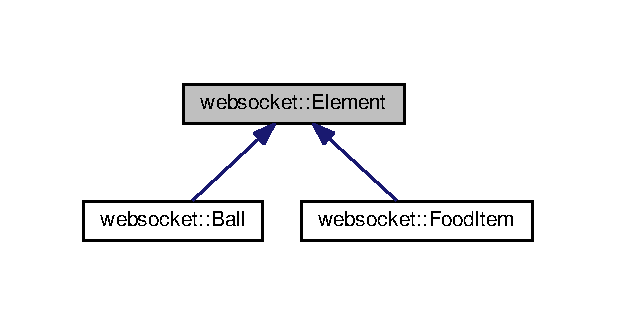
\includegraphics[width=296pt]{classwebsocket_1_1Element__inherit__graph}
\end{center}
\end{figure}
\subsection*{Public Member Functions}
\begin{DoxyCompactItemize}
\item 
\hyperlink{classwebsocket_1_1Element_a6d6b671ae2f922c12c0a64a94bd669fb}{Element} (double \&x, double \&y, double \&radius)
\item 
\hyperlink{classwebsocket_1_1Element_a4a249effc753deac10eb2eb7fc80c759}{$\sim$\+Element} ()=default
\item 
\hyperlink{classwebsocket_1_1Element_a7b16c1d2898cb3d1db6b5305045838bf}{Element} (const \hyperlink{classwebsocket_1_1Element}{Element} \&other)=default
\item 
\hyperlink{classwebsocket_1_1Element}{Element} \& \hyperlink{classwebsocket_1_1Element_a3c188d2039c89735c2d5e09123266397}{operator=} (const \hyperlink{classwebsocket_1_1Element}{Element} \&other)=default
\item 
double \hyperlink{classwebsocket_1_1Element_adb9892f7b44913049e0c771816efd7a4}{get\+Id} ()
\item 
double \hyperlink{classwebsocket_1_1Element_a6102d0b4ccbad0194ee393fa5341cabc}{getX} ()
\item 
double \hyperlink{classwebsocket_1_1Element_a597f360c2c593a6610a2a9103d5e876b}{getY} ()
\item 
double \hyperlink{classwebsocket_1_1Element_a895b218f0ec4d2d4e2164c2531a8ffe3}{get\+Radius} ()
\item 
void \hyperlink{classwebsocket_1_1Element_aba38ddf15ce77e2e79bce80cf38947db}{setX} (const double \&x)
\item 
void \hyperlink{classwebsocket_1_1Element_ab05d0ca40f4d1a79d52cb31c5b4f789b}{setY} (const double \&y)
\item 
void \hyperlink{classwebsocket_1_1Element_a4ad55c97fa8f5684af5bc25780450db1}{set\+Radius} (double \&\&radius)
\item 
virtual \hyperlink{namespacewebsocket_aec8d52893bdf524a1412533a63b006a3}{player\+\_\+ptr} \hyperlink{classwebsocket_1_1Element_a28027c861e94306a7666d839db910f2a}{get\+Owner} ()=0
\end{DoxyCompactItemize}
\subsection*{Protected Attributes}
\begin{DoxyCompactItemize}
\item 
double \hyperlink{classwebsocket_1_1Element_adb51cfefd07378c784d30340c449a224}{x\+\_\+}
\item 
double \hyperlink{classwebsocket_1_1Element_a61ea05afb0180339005d1c96786a60ce}{y\+\_\+}
\item 
double \hyperlink{classwebsocket_1_1Element_aec20349985f8c1bc19d6f686658e6c62}{radius\+\_\+}
\end{DoxyCompactItemize}
\subsection*{Private Attributes}
\begin{DoxyCompactItemize}
\item 
const int \hyperlink{classwebsocket_1_1Element_a0cb8ab190a65134d23ff3bf4054865eb}{id\+\_\+}
\end{DoxyCompactItemize}
\subsection*{Static Private Attributes}
\begin{DoxyCompactItemize}
\item 
static int \hyperlink{classwebsocket_1_1Element_af6fa7171fdd68176492397d9706947b3}{id\+Count\+\_\+}
\end{DoxyCompactItemize}


\subsection{Constructor \& Destructor Documentation}
\index{websocket\+::\+Element@{websocket\+::\+Element}!Element@{Element}}
\index{Element@{Element}!websocket\+::\+Element@{websocket\+::\+Element}}
\subsubsection[{\texorpdfstring{Element(double \&x, double \&y, double \&radius)}{Element(double &x, double &y, double &radius)}}]{\setlength{\rightskip}{0pt plus 5cm}websocket\+::\+Element\+::\+Element (
\begin{DoxyParamCaption}
\item[{double \&}]{x, }
\item[{double \&}]{y, }
\item[{double \&}]{radius}
\end{DoxyParamCaption}
)}\hypertarget{classwebsocket_1_1Element_a6d6b671ae2f922c12c0a64a94bd669fb}{}\label{classwebsocket_1_1Element_a6d6b671ae2f922c12c0a64a94bd669fb}
\index{websocket\+::\+Element@{websocket\+::\+Element}!````~Element@{$\sim$\+Element}}
\index{````~Element@{$\sim$\+Element}!websocket\+::\+Element@{websocket\+::\+Element}}
\subsubsection[{\texorpdfstring{$\sim$\+Element()=default}{~Element()=default}}]{\setlength{\rightskip}{0pt plus 5cm}websocket\+::\+Element\+::$\sim$\+Element (
\begin{DoxyParamCaption}
{}
\end{DoxyParamCaption}
)\hspace{0.3cm}{\ttfamily [default]}}\hypertarget{classwebsocket_1_1Element_a4a249effc753deac10eb2eb7fc80c759}{}\label{classwebsocket_1_1Element_a4a249effc753deac10eb2eb7fc80c759}
\index{websocket\+::\+Element@{websocket\+::\+Element}!Element@{Element}}
\index{Element@{Element}!websocket\+::\+Element@{websocket\+::\+Element}}
\subsubsection[{\texorpdfstring{Element(const Element \&other)=default}{Element(const Element &other)=default}}]{\setlength{\rightskip}{0pt plus 5cm}websocket\+::\+Element\+::\+Element (
\begin{DoxyParamCaption}
\item[{const {\bf Element} \&}]{other}
\end{DoxyParamCaption}
)\hspace{0.3cm}{\ttfamily [default]}}\hypertarget{classwebsocket_1_1Element_a7b16c1d2898cb3d1db6b5305045838bf}{}\label{classwebsocket_1_1Element_a7b16c1d2898cb3d1db6b5305045838bf}


\subsection{Member Function Documentation}
\index{websocket\+::\+Element@{websocket\+::\+Element}!get\+Id@{get\+Id}}
\index{get\+Id@{get\+Id}!websocket\+::\+Element@{websocket\+::\+Element}}
\subsubsection[{\texorpdfstring{get\+Id()}{getId()}}]{\setlength{\rightskip}{0pt plus 5cm}double websocket\+::\+Element\+::get\+Id (
\begin{DoxyParamCaption}
{}
\end{DoxyParamCaption}
)\hspace{0.3cm}{\ttfamily [inline]}}\hypertarget{classwebsocket_1_1Element_adb9892f7b44913049e0c771816efd7a4}{}\label{classwebsocket_1_1Element_adb9892f7b44913049e0c771816efd7a4}
\index{websocket\+::\+Element@{websocket\+::\+Element}!get\+Owner@{get\+Owner}}
\index{get\+Owner@{get\+Owner}!websocket\+::\+Element@{websocket\+::\+Element}}
\subsubsection[{\texorpdfstring{get\+Owner()=0}{getOwner()=0}}]{\setlength{\rightskip}{0pt plus 5cm}virtual {\bf player\+\_\+ptr} websocket\+::\+Element\+::get\+Owner (
\begin{DoxyParamCaption}
{}
\end{DoxyParamCaption}
)\hspace{0.3cm}{\ttfamily [pure virtual]}}\hypertarget{classwebsocket_1_1Element_a28027c861e94306a7666d839db910f2a}{}\label{classwebsocket_1_1Element_a28027c861e94306a7666d839db910f2a}


Implemented in \hyperlink{classwebsocket_1_1Ball_a7c418a9c85d74e6644d9ffa294c8df74}{websocket\+::\+Ball}, and \hyperlink{classwebsocket_1_1FoodItem_a4c39197cbbe8563fe94c4fd886a897e0}{websocket\+::\+Food\+Item}.

\index{websocket\+::\+Element@{websocket\+::\+Element}!get\+Radius@{get\+Radius}}
\index{get\+Radius@{get\+Radius}!websocket\+::\+Element@{websocket\+::\+Element}}
\subsubsection[{\texorpdfstring{get\+Radius()}{getRadius()}}]{\setlength{\rightskip}{0pt plus 5cm}double websocket\+::\+Element\+::get\+Radius (
\begin{DoxyParamCaption}
{}
\end{DoxyParamCaption}
)\hspace{0.3cm}{\ttfamily [inline]}}\hypertarget{classwebsocket_1_1Element_a895b218f0ec4d2d4e2164c2531a8ffe3}{}\label{classwebsocket_1_1Element_a895b218f0ec4d2d4e2164c2531a8ffe3}
\index{websocket\+::\+Element@{websocket\+::\+Element}!getX@{getX}}
\index{getX@{getX}!websocket\+::\+Element@{websocket\+::\+Element}}
\subsubsection[{\texorpdfstring{get\+X()}{getX()}}]{\setlength{\rightskip}{0pt plus 5cm}double websocket\+::\+Element\+::getX (
\begin{DoxyParamCaption}
{}
\end{DoxyParamCaption}
)\hspace{0.3cm}{\ttfamily [inline]}}\hypertarget{classwebsocket_1_1Element_a6102d0b4ccbad0194ee393fa5341cabc}{}\label{classwebsocket_1_1Element_a6102d0b4ccbad0194ee393fa5341cabc}
\index{websocket\+::\+Element@{websocket\+::\+Element}!getY@{getY}}
\index{getY@{getY}!websocket\+::\+Element@{websocket\+::\+Element}}
\subsubsection[{\texorpdfstring{get\+Y()}{getY()}}]{\setlength{\rightskip}{0pt plus 5cm}double websocket\+::\+Element\+::getY (
\begin{DoxyParamCaption}
{}
\end{DoxyParamCaption}
)\hspace{0.3cm}{\ttfamily [inline]}}\hypertarget{classwebsocket_1_1Element_a597f360c2c593a6610a2a9103d5e876b}{}\label{classwebsocket_1_1Element_a597f360c2c593a6610a2a9103d5e876b}
\index{websocket\+::\+Element@{websocket\+::\+Element}!operator=@{operator=}}
\index{operator=@{operator=}!websocket\+::\+Element@{websocket\+::\+Element}}
\subsubsection[{\texorpdfstring{operator=(const Element \&other)=default}{operator=(const Element &other)=default}}]{\setlength{\rightskip}{0pt plus 5cm}{\bf Element}\& websocket\+::\+Element\+::operator= (
\begin{DoxyParamCaption}
\item[{const {\bf Element} \&}]{other}
\end{DoxyParamCaption}
)\hspace{0.3cm}{\ttfamily [default]}}\hypertarget{classwebsocket_1_1Element_a3c188d2039c89735c2d5e09123266397}{}\label{classwebsocket_1_1Element_a3c188d2039c89735c2d5e09123266397}
\index{websocket\+::\+Element@{websocket\+::\+Element}!set\+Radius@{set\+Radius}}
\index{set\+Radius@{set\+Radius}!websocket\+::\+Element@{websocket\+::\+Element}}
\subsubsection[{\texorpdfstring{set\+Radius(double \&\&radius)}{setRadius(double &&radius)}}]{\setlength{\rightskip}{0pt plus 5cm}void websocket\+::\+Element\+::set\+Radius (
\begin{DoxyParamCaption}
\item[{double \&\&}]{radius}
\end{DoxyParamCaption}
)\hspace{0.3cm}{\ttfamily [inline]}}\hypertarget{classwebsocket_1_1Element_a4ad55c97fa8f5684af5bc25780450db1}{}\label{classwebsocket_1_1Element_a4ad55c97fa8f5684af5bc25780450db1}
\index{websocket\+::\+Element@{websocket\+::\+Element}!setX@{setX}}
\index{setX@{setX}!websocket\+::\+Element@{websocket\+::\+Element}}
\subsubsection[{\texorpdfstring{set\+X(const double \&x)}{setX(const double &x)}}]{\setlength{\rightskip}{0pt plus 5cm}void websocket\+::\+Element\+::setX (
\begin{DoxyParamCaption}
\item[{const double \&}]{x}
\end{DoxyParamCaption}
)\hspace{0.3cm}{\ttfamily [inline]}}\hypertarget{classwebsocket_1_1Element_aba38ddf15ce77e2e79bce80cf38947db}{}\label{classwebsocket_1_1Element_aba38ddf15ce77e2e79bce80cf38947db}
\index{websocket\+::\+Element@{websocket\+::\+Element}!setY@{setY}}
\index{setY@{setY}!websocket\+::\+Element@{websocket\+::\+Element}}
\subsubsection[{\texorpdfstring{set\+Y(const double \&y)}{setY(const double &y)}}]{\setlength{\rightskip}{0pt plus 5cm}void websocket\+::\+Element\+::setY (
\begin{DoxyParamCaption}
\item[{const double \&}]{y}
\end{DoxyParamCaption}
)\hspace{0.3cm}{\ttfamily [inline]}}\hypertarget{classwebsocket_1_1Element_ab05d0ca40f4d1a79d52cb31c5b4f789b}{}\label{classwebsocket_1_1Element_ab05d0ca40f4d1a79d52cb31c5b4f789b}


\subsection{Member Data Documentation}
\index{websocket\+::\+Element@{websocket\+::\+Element}!id\+\_\+@{id\+\_\+}}
\index{id\+\_\+@{id\+\_\+}!websocket\+::\+Element@{websocket\+::\+Element}}
\subsubsection[{\texorpdfstring{id\+\_\+}{id_}}]{\setlength{\rightskip}{0pt plus 5cm}const int websocket\+::\+Element\+::id\+\_\+\hspace{0.3cm}{\ttfamily [private]}}\hypertarget{classwebsocket_1_1Element_a0cb8ab190a65134d23ff3bf4054865eb}{}\label{classwebsocket_1_1Element_a0cb8ab190a65134d23ff3bf4054865eb}
\index{websocket\+::\+Element@{websocket\+::\+Element}!id\+Count\+\_\+@{id\+Count\+\_\+}}
\index{id\+Count\+\_\+@{id\+Count\+\_\+}!websocket\+::\+Element@{websocket\+::\+Element}}
\subsubsection[{\texorpdfstring{id\+Count\+\_\+}{idCount_}}]{\setlength{\rightskip}{0pt plus 5cm}int websocket\+::\+Element\+::id\+Count\+\_\+\hspace{0.3cm}{\ttfamily [static]}, {\ttfamily [private]}}\hypertarget{classwebsocket_1_1Element_af6fa7171fdd68176492397d9706947b3}{}\label{classwebsocket_1_1Element_af6fa7171fdd68176492397d9706947b3}
\index{websocket\+::\+Element@{websocket\+::\+Element}!radius\+\_\+@{radius\+\_\+}}
\index{radius\+\_\+@{radius\+\_\+}!websocket\+::\+Element@{websocket\+::\+Element}}
\subsubsection[{\texorpdfstring{radius\+\_\+}{radius_}}]{\setlength{\rightskip}{0pt plus 5cm}double websocket\+::\+Element\+::radius\+\_\+\hspace{0.3cm}{\ttfamily [protected]}}\hypertarget{classwebsocket_1_1Element_aec20349985f8c1bc19d6f686658e6c62}{}\label{classwebsocket_1_1Element_aec20349985f8c1bc19d6f686658e6c62}
\index{websocket\+::\+Element@{websocket\+::\+Element}!x\+\_\+@{x\+\_\+}}
\index{x\+\_\+@{x\+\_\+}!websocket\+::\+Element@{websocket\+::\+Element}}
\subsubsection[{\texorpdfstring{x\+\_\+}{x_}}]{\setlength{\rightskip}{0pt plus 5cm}double websocket\+::\+Element\+::x\+\_\+\hspace{0.3cm}{\ttfamily [protected]}}\hypertarget{classwebsocket_1_1Element_adb51cfefd07378c784d30340c449a224}{}\label{classwebsocket_1_1Element_adb51cfefd07378c784d30340c449a224}
\index{websocket\+::\+Element@{websocket\+::\+Element}!y\+\_\+@{y\+\_\+}}
\index{y\+\_\+@{y\+\_\+}!websocket\+::\+Element@{websocket\+::\+Element}}
\subsubsection[{\texorpdfstring{y\+\_\+}{y_}}]{\setlength{\rightskip}{0pt plus 5cm}double websocket\+::\+Element\+::y\+\_\+\hspace{0.3cm}{\ttfamily [protected]}}\hypertarget{classwebsocket_1_1Element_a61ea05afb0180339005d1c96786a60ce}{}\label{classwebsocket_1_1Element_a61ea05afb0180339005d1c96786a60ce}


The documentation for this class was generated from the following files\+:\begin{DoxyCompactItemize}
\item 
\hyperlink{element_8hpp}{element.\+hpp}\item 
\hyperlink{element_8cpp}{element.\+cpp}\end{DoxyCompactItemize}

\hypertarget{classwebsocket_1_1FoodItem}{}\section{websocket\+:\+:Food\+Item Class Reference}
\label{classwebsocket_1_1FoodItem}\index{websocket\+::\+Food\+Item@{websocket\+::\+Food\+Item}}


{\ttfamily \#include $<$food\+Item.\+hpp$>$}



Inheritance diagram for websocket\+:\+:Food\+Item\+:\nopagebreak
\begin{figure}[H]
\begin{center}
\leavevmode
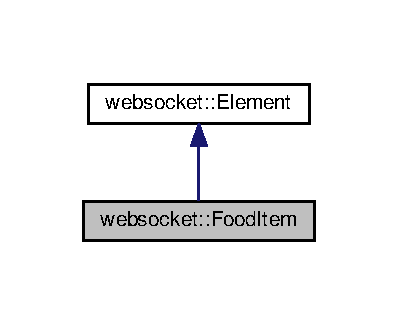
\includegraphics[width=191pt]{classwebsocket_1_1FoodItem__inherit__graph}
\end{center}
\end{figure}


Collaboration diagram for websocket\+:\+:Food\+Item\+:\nopagebreak
\begin{figure}[H]
\begin{center}
\leavevmode
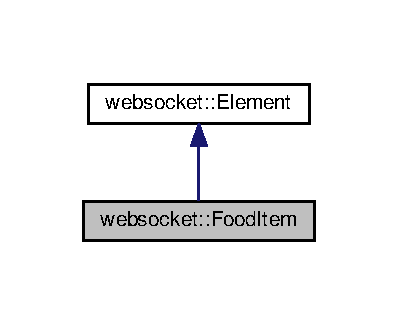
\includegraphics[width=191pt]{classwebsocket_1_1FoodItem__coll__graph}
\end{center}
\end{figure}
\subsection*{Public Member Functions}
\begin{DoxyCompactItemize}
\item 
\hyperlink{classwebsocket_1_1FoodItem_a2e34bb4440281bf3f8c01c1952c58d39}{Food\+Item} (double \&x, double \&y, double radius)
\item 
\hyperlink{classwebsocket_1_1FoodItem_a870abf88e3f80d5218fa017e52601d60}{$\sim$\+Food\+Item} ()=default
\item 
\hyperlink{classwebsocket_1_1FoodItem_ac69bbf80ef72ce4bdb8dd73be2066d10}{Food\+Item} (const \hyperlink{classwebsocket_1_1FoodItem}{Food\+Item} \&other)=default
\item 
\hyperlink{classwebsocket_1_1FoodItem}{Food\+Item} \& \hyperlink{classwebsocket_1_1FoodItem_ac3726c11be41df9a1dbbab983d35bd43}{operator=} (const \hyperlink{classwebsocket_1_1FoodItem}{Food\+Item} \&other)=default
\item 
virtual \hyperlink{namespacewebsocket_aec8d52893bdf524a1412533a63b006a3}{player\+\_\+ptr} \hyperlink{classwebsocket_1_1FoodItem_a4c39197cbbe8563fe94c4fd886a897e0}{get\+Owner} ()
\end{DoxyCompactItemize}
\subsection*{Additional Inherited Members}


\subsection{Constructor \& Destructor Documentation}
\index{websocket\+::\+Food\+Item@{websocket\+::\+Food\+Item}!Food\+Item@{Food\+Item}}
\index{Food\+Item@{Food\+Item}!websocket\+::\+Food\+Item@{websocket\+::\+Food\+Item}}
\subsubsection[{\texorpdfstring{Food\+Item(double \&x, double \&y, double radius)}{FoodItem(double &x, double &y, double radius)}}]{\setlength{\rightskip}{0pt plus 5cm}websocket\+::\+Food\+Item\+::\+Food\+Item (
\begin{DoxyParamCaption}
\item[{double \&}]{x, }
\item[{double \&}]{y, }
\item[{double}]{radius}
\end{DoxyParamCaption}
)}\hypertarget{classwebsocket_1_1FoodItem_a2e34bb4440281bf3f8c01c1952c58d39}{}\label{classwebsocket_1_1FoodItem_a2e34bb4440281bf3f8c01c1952c58d39}
\index{websocket\+::\+Food\+Item@{websocket\+::\+Food\+Item}!````~Food\+Item@{$\sim$\+Food\+Item}}
\index{````~Food\+Item@{$\sim$\+Food\+Item}!websocket\+::\+Food\+Item@{websocket\+::\+Food\+Item}}
\subsubsection[{\texorpdfstring{$\sim$\+Food\+Item()=default}{~FoodItem()=default}}]{\setlength{\rightskip}{0pt plus 5cm}websocket\+::\+Food\+Item\+::$\sim$\+Food\+Item (
\begin{DoxyParamCaption}
{}
\end{DoxyParamCaption}
)\hspace{0.3cm}{\ttfamily [default]}}\hypertarget{classwebsocket_1_1FoodItem_a870abf88e3f80d5218fa017e52601d60}{}\label{classwebsocket_1_1FoodItem_a870abf88e3f80d5218fa017e52601d60}
\index{websocket\+::\+Food\+Item@{websocket\+::\+Food\+Item}!Food\+Item@{Food\+Item}}
\index{Food\+Item@{Food\+Item}!websocket\+::\+Food\+Item@{websocket\+::\+Food\+Item}}
\subsubsection[{\texorpdfstring{Food\+Item(const Food\+Item \&other)=default}{FoodItem(const FoodItem &other)=default}}]{\setlength{\rightskip}{0pt plus 5cm}websocket\+::\+Food\+Item\+::\+Food\+Item (
\begin{DoxyParamCaption}
\item[{const {\bf Food\+Item} \&}]{other}
\end{DoxyParamCaption}
)\hspace{0.3cm}{\ttfamily [default]}}\hypertarget{classwebsocket_1_1FoodItem_ac69bbf80ef72ce4bdb8dd73be2066d10}{}\label{classwebsocket_1_1FoodItem_ac69bbf80ef72ce4bdb8dd73be2066d10}


\subsection{Member Function Documentation}
\index{websocket\+::\+Food\+Item@{websocket\+::\+Food\+Item}!get\+Owner@{get\+Owner}}
\index{get\+Owner@{get\+Owner}!websocket\+::\+Food\+Item@{websocket\+::\+Food\+Item}}
\subsubsection[{\texorpdfstring{get\+Owner()}{getOwner()}}]{\setlength{\rightskip}{0pt plus 5cm}virtual {\bf player\+\_\+ptr} websocket\+::\+Food\+Item\+::get\+Owner (
\begin{DoxyParamCaption}
{}
\end{DoxyParamCaption}
)\hspace{0.3cm}{\ttfamily [inline]}, {\ttfamily [virtual]}}\hypertarget{classwebsocket_1_1FoodItem_a4c39197cbbe8563fe94c4fd886a897e0}{}\label{classwebsocket_1_1FoodItem_a4c39197cbbe8563fe94c4fd886a897e0}


Implements \hyperlink{classwebsocket_1_1Element_a28027c861e94306a7666d839db910f2a}{websocket\+::\+Element}.

\index{websocket\+::\+Food\+Item@{websocket\+::\+Food\+Item}!operator=@{operator=}}
\index{operator=@{operator=}!websocket\+::\+Food\+Item@{websocket\+::\+Food\+Item}}
\subsubsection[{\texorpdfstring{operator=(const Food\+Item \&other)=default}{operator=(const FoodItem &other)=default}}]{\setlength{\rightskip}{0pt plus 5cm}{\bf Food\+Item}\& websocket\+::\+Food\+Item\+::operator= (
\begin{DoxyParamCaption}
\item[{const {\bf Food\+Item} \&}]{other}
\end{DoxyParamCaption}
)\hspace{0.3cm}{\ttfamily [default]}}\hypertarget{classwebsocket_1_1FoodItem_ac3726c11be41df9a1dbbab983d35bd43}{}\label{classwebsocket_1_1FoodItem_ac3726c11be41df9a1dbbab983d35bd43}


The documentation for this class was generated from the following files\+:\begin{DoxyCompactItemize}
\item 
\hyperlink{foodItem_8hpp}{food\+Item.\+hpp}\item 
\hyperlink{foodItem_8cpp}{food\+Item.\+cpp}\end{DoxyCompactItemize}

\hypertarget{classwebsocket_1_1GameBoard}{}\section{websocket\+:\+:Game\+Board Class Reference}
\label{classwebsocket_1_1GameBoard}\index{websocket\+::\+Game\+Board@{websocket\+::\+Game\+Board}}


{\ttfamily \#include $<$game\+\_\+board.\+hpp$>$}



Inheritance diagram for websocket\+:\+:Game\+Board\+:
\nopagebreak
\begin{figure}[H]
\begin{center}
\leavevmode
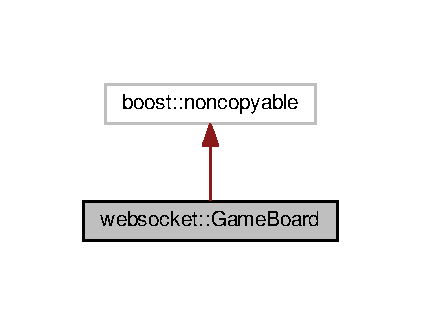
\includegraphics[width=202pt]{classwebsocket_1_1GameBoard__inherit__graph}
\end{center}
\end{figure}


Collaboration diagram for websocket\+:\+:Game\+Board\+:
\nopagebreak
\begin{figure}[H]
\begin{center}
\leavevmode
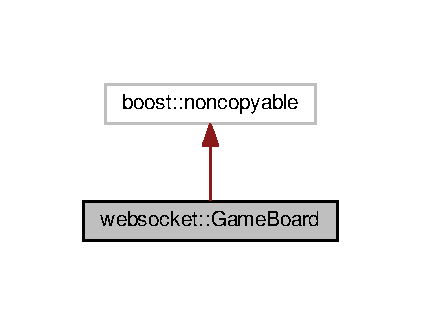
\includegraphics[width=202pt]{classwebsocket_1_1GameBoard__coll__graph}
\end{center}
\end{figure}
\subsection*{Public Member Functions}
\begin{DoxyCompactItemize}
\item 
\hyperlink{classwebsocket_1_1GameBoard_a8093c83a31dd38e3edf1bc07de4b060a}{Game\+Board} ()
\item 
void \hyperlink{classwebsocket_1_1GameBoard_a3ca61a3da72869402a6e1702a99faa76}{join} (\hyperlink{namespacewebsocket_aec8d52893bdf524a1412533a63b006a3}{player\+\_\+ptr} participant)
\begin{DoxyCompactList}\small\item\em Join the game\+\_\+board. \end{DoxyCompactList}\item 
void \hyperlink{classwebsocket_1_1GameBoard_a2f3f0eb3fb2fbe6303426c1bc8d3fff7}{leave} (\hyperlink{namespacewebsocket_aec8d52893bdf524a1412533a63b006a3}{player\+\_\+ptr} participant)
\begin{DoxyCompactList}\small\item\em Leave the game\+\_\+board. \end{DoxyCompactList}\item 
void \hyperlink{classwebsocket_1_1GameBoard_a0ed4b13ba573956d8aebaf8f5c208fa0}{deliver} (const \hyperlink{structwebsocket_1_1Dataframe}{Dataframe} \&msg, \hyperlink{namespacewebsocket_aec8d52893bdf524a1412533a63b006a3}{player\+\_\+ptr} source)
\begin{DoxyCompactList}\small\item\em Deliver a chat message to all participant in the game\+\_\+board. \end{DoxyCompactList}\end{DoxyCompactItemize}
\subsection*{Static Public Member Functions}
\begin{DoxyCompactItemize}
\item 
static int \hyperlink{classwebsocket_1_1GameBoard_a3e8a7dec314f570a1d8cf92d4a711bd5}{get\+MapX} ()
\begin{DoxyCompactList}\small\item\em return map dimentions \end{DoxyCompactList}\item 
static int \hyperlink{classwebsocket_1_1GameBoard_a4f2dd5ab46f74a995388687dd6a5f440}{get\+MapY} ()
\end{DoxyCompactItemize}
\subsection*{Private Types}
\begin{DoxyCompactItemize}
\item 
enum \{ \hyperlink{classwebsocket_1_1GameBoard_a84b7265b5db0109546eeadc332b10254a1a669a5c5c208eebeb228bd6cbe3611b}{max\+\_\+recent\+\_\+msgs} = 1000
 \}
\item 
typedef std\+::set$<$ std\+::pair$<$ int, int $>$ $>$ \hyperlink{classwebsocket_1_1GameBoard_ab68a03a083cfa75e7d5b21fe0c13eda3}{occupied\+\_\+pos}
\item 
typedef std\+::map$<$ \hyperlink{namespacewebsocket_aec8d52893bdf524a1412533a63b006a3}{player\+\_\+ptr}, \hyperlink{namespacewebsocket_aae1d9cf317a0fb0b83bdfc2f92df77c7}{ball\+\_\+ptr} $>$ \hyperlink{classwebsocket_1_1GameBoard_a49ec88dacda0efb3448649503967e07d}{balls\+\_\+container}
\item 
typedef std\+::map$<$ int, \hyperlink{namespacewebsocket_a1f36ba91b301b228fa9e9f812883050c}{element\+\_\+ptr} $>$ \hyperlink{classwebsocket_1_1GameBoard_a6340e99ab84e0fc9ee504f5874073c0c}{elements\+\_\+container}
\end{DoxyCompactItemize}
\subsection*{Private Member Functions}
\begin{DoxyCompactItemize}
\item 
void \hyperlink{classwebsocket_1_1GameBoard_a66d8b6bfa24c4902896acff4e49f3dc5}{deliver} (const \hyperlink{structwebsocket_1_1Dataframe}{Dataframe} \&msg)
\begin{DoxyCompactList}\small\item\em Deliver a message to all participant in the game\+\_\+board. \end{DoxyCompactList}\item 
void \hyperlink{classwebsocket_1_1GameBoard_a9d97f5e5069d0501ea37cb819d481dd0}{update\+Participants} ()
\begin{DoxyCompactList}\small\item\em Update a number of connected participants. \end{DoxyCompactList}\item 
void \hyperlink{classwebsocket_1_1GameBoard_a4bcaa4bcf0a260efa6baffec4e72990e}{add\+N\+Food\+Item} (int n)
\begin{DoxyCompactList}\small\item\em Methods of game logic. \end{DoxyCompactList}\item 
\hyperlink{namespacewebsocket_a198017789b8c5fa32315a12d5ce97869}{food\+\_\+ptr} \hyperlink{classwebsocket_1_1GameBoard_a3a0cacc2c9a90a5752a8b29ea243c9af}{get\+Food} (double \&x, double \&y)
\begin{DoxyCompactList}\small\item\em create new food\+Item \end{DoxyCompactList}\item 
void \hyperlink{classwebsocket_1_1GameBoard_a9bf63429b6e4ef6cb652eab0224fba4f}{erase\+Food} (int id)
\begin{DoxyCompactList}\small\item\em erase food\+Item from collection and informs other players \end{DoxyCompactList}\item 
void \hyperlink{classwebsocket_1_1GameBoard_a9067bf26d8aae3e4f325d866247e0951}{add\+New\+Ball} (\hyperlink{namespacewebsocket_aec8d52893bdf524a1412533a63b006a3}{player\+\_\+ptr} participant, std\+::string nick)
\begin{DoxyCompactList}\small\item\em add new ball for new player and update other players \end{DoxyCompactList}\item 
\hyperlink{namespacewebsocket_aae1d9cf317a0fb0b83bdfc2f92df77c7}{ball\+\_\+ptr} \hyperlink{classwebsocket_1_1GameBoard_ac9ebf0c8fc6a76a60fcc83d60719b161}{get\+Ball} (double \&x, double \&y, double radius)
\begin{DoxyCompactList}\small\item\em create new ball for player \end{DoxyCompactList}\item 
void \hyperlink{classwebsocket_1_1GameBoard_a581a9aeb4f1e70892a70a238bba6469a}{send\+Game\+State} (\hyperlink{namespacewebsocket_aec8d52893bdf524a1412533a63b006a3}{player\+\_\+ptr} participant)
\begin{DoxyCompactList}\small\item\em Sends balls and foods position to players. \end{DoxyCompactList}\item 
void \hyperlink{classwebsocket_1_1GameBoard_ac9130252983df425bcefd450f4aa8742}{erase\+Ball} (\hyperlink{namespacewebsocket_aec8d52893bdf524a1412533a63b006a3}{player\+\_\+ptr} participant)
\begin{DoxyCompactList}\small\item\em delete ball and update players \end{DoxyCompactList}\item 
void \hyperlink{classwebsocket_1_1GameBoard_a40aed2036d1065d0bfa24d4e84da1418}{process\+Movement} (const \hyperlink{structwebsocket_1_1Dataframe}{Dataframe} \&msg, \hyperlink{namespacewebsocket_aec8d52893bdf524a1412533a63b006a3}{player\+\_\+ptr} source)
\begin{DoxyCompactList}\small\item\em main movement processing \end{DoxyCompactList}\item 
void \hyperlink{classwebsocket_1_1GameBoard_a20af876986152e2c4db78174d186d2b6}{is\+Nick\+Valid} (const \hyperlink{structwebsocket_1_1Dataframe}{Dataframe} \&msg, \hyperlink{namespacewebsocket_aec8d52893bdf524a1412533a63b006a3}{player\+\_\+ptr} source)
\begin{DoxyCompactList}\small\item\em method of initial handshake -\/ checks validity of inserted user nick \end{DoxyCompactList}\item 
void \hyperlink{classwebsocket_1_1GameBoard_ad6da3630e77cf3da0563072e5c1ec162}{add\+Player\+To\+Game} (const \hyperlink{structwebsocket_1_1Dataframe}{Dataframe} \&msg, \hyperlink{namespacewebsocket_aec8d52893bdf524a1412533a63b006a3}{player\+\_\+ptr} source)
\begin{DoxyCompactList}\small\item\em on valid nick defines set of methods used to initiate the game \end{DoxyCompactList}\item 
void \hyperlink{classwebsocket_1_1GameBoard_a93379a2caec9ae069ffef81472e608f9}{send\+Map\+Size} (\hyperlink{namespacewebsocket_aec8d52893bdf524a1412533a63b006a3}{player\+\_\+ptr} source)
\begin{DoxyCompactList}\small\item\em sends map dimensions to the new player \end{DoxyCompactList}\end{DoxyCompactItemize}
\subsection*{Private Attributes}
\begin{DoxyCompactItemize}
\item 
std\+::set$<$ \hyperlink{namespacewebsocket_aec8d52893bdf524a1412533a63b006a3}{player\+\_\+ptr} $>$ \hyperlink{classwebsocket_1_1GameBoard_a49ad7c4c31e144021a4c7e12c73d0433}{participants\+\_\+}
\item 
\hyperlink{namespacewebsocket_ae3fdf29bb367b5baf5be703253a4edfa}{message\+\_\+queue} \hyperlink{classwebsocket_1_1GameBoard_a87c11dd6d2f39fa8b0100059c27179a7}{recent\+\_\+msgs\+\_\+}
\end{DoxyCompactItemize}
\subsection*{Static Private Attributes}
\begin{DoxyCompactItemize}
\item 
static const int \hyperlink{classwebsocket_1_1GameBoard_a02d0925d31cf26c6853cbb39de6f051c}{map\+X\+\_\+} \{10000\}
\item 
static const int \hyperlink{classwebsocket_1_1GameBoard_a60432d0d991c965b75ad2557e9610425}{map\+Y\+\_\+} \{10000\}
\item 
static const double \hyperlink{classwebsocket_1_1GameBoard_a1bedb4dff215404c5574f064c68789c8}{food\+Item\+Marigin\+\_\+} \{5\}
\item 
static const double \hyperlink{classwebsocket_1_1GameBoard_add182baa81ccbe72610eebacdb0b8dd6}{ball\+Marigin\+\_\+} \{10\}
\item 
static const int \hyperlink{classwebsocket_1_1GameBoard_ad2f7ea28ea20d8d16f06135cc09b92e1}{initial\+Food\+\_\+} \{350\}
\item 
static const int \hyperlink{classwebsocket_1_1GameBoard_aad2445e5c98fe42f37e71c15ca3c57c9}{new\+Player\+Food\+\_\+} \{5\}
\item 
static const int \hyperlink{classwebsocket_1_1GameBoard_a80f3a0b794866a7e3c9dac0bf15ba14a}{initial\+Food\+Params\+\_\+} \{1\}
\item 
static const int \hyperlink{classwebsocket_1_1GameBoard_a7277b9cbeca558d4bcfad3c24d185336}{food\+Radius\+\_\+} \{3\}
\item 
static const int \hyperlink{classwebsocket_1_1GameBoard_a8fe312bcfc33ae3d624a0fdb02f40622}{on\+Eaten\+New\+Items\+\_\+} \{1\}
\item 
static const int \hyperlink{classwebsocket_1_1GameBoard_a0644b0415ab9a8f4a260e277fca79e1a}{init\+Ball\+Radius\+\_\+} \{20\}
\item 
static \hyperlink{classwebsocket_1_1GameBoard_ab68a03a083cfa75e7d5b21fe0c13eda3}{occupied\+\_\+pos} \hyperlink{classwebsocket_1_1GameBoard_aca1010defacfdd0ea5f032035ce7105e}{occupied\+Pos\+\_\+}
\item 
static \hyperlink{classwebsocket_1_1GameBoard_a49ec88dacda0efb3448649503967e07d}{balls\+\_\+container} \hyperlink{classwebsocket_1_1GameBoard_a8bdb65edb9742890aa150d5c7c5b7209}{balls\+\_\+}
\item 
static \hyperlink{classwebsocket_1_1GameBoard_a6340e99ab84e0fc9ee504f5874073c0c}{elements\+\_\+container} \hyperlink{classwebsocket_1_1GameBoard_a56fd12d10af951e1f6a42a18f4ccfe35}{elements\+\_\+}
\item 
static const std\+::string \hyperlink{classwebsocket_1_1GameBoard_a27fc2053eae7a0bdc4ec6cb7ff92502e}{message\+Op\+\_\+} = \char`\"{}message\char`\"{}
\item 
static const std\+::string \hyperlink{classwebsocket_1_1GameBoard_ac5eba2bf19bde163ea767906c8e2c61c}{movement\+Op\+\_\+} = \char`\"{}move\char`\"{}
\item 
static const std\+::string \hyperlink{classwebsocket_1_1GameBoard_a55afbbb9d15f4815427d2f20ca6674cd}{nick\+Check\+Op\+\_\+} = \char`\"{}new\+Player\+Name\char`\"{}
\item 
static const std\+::string \hyperlink{classwebsocket_1_1GameBoard_af28eae4479ca907c062495b7ec2925c1}{new\+Player\+Status\+Op\+\_\+} = \char`\"{}new\+Player\+Status\char`\"{}
\end{DoxyCompactItemize}


\subsection{Member Typedef Documentation}
\index{websocket\+::\+Game\+Board@{websocket\+::\+Game\+Board}!balls\+\_\+container@{balls\+\_\+container}}
\index{balls\+\_\+container@{balls\+\_\+container}!websocket\+::\+Game\+Board@{websocket\+::\+Game\+Board}}
\subsubsection[{\texorpdfstring{balls\+\_\+container}{balls_container}}]{\setlength{\rightskip}{0pt plus 5cm}typedef std\+::map$<${\bf player\+\_\+ptr},{\bf ball\+\_\+ptr} $>$ {\bf websocket\+::\+Game\+Board\+::balls\+\_\+container}\hspace{0.3cm}{\ttfamily [private]}}\hypertarget{classwebsocket_1_1GameBoard_a49ec88dacda0efb3448649503967e07d}{}\label{classwebsocket_1_1GameBoard_a49ec88dacda0efb3448649503967e07d}
\index{websocket\+::\+Game\+Board@{websocket\+::\+Game\+Board}!elements\+\_\+container@{elements\+\_\+container}}
\index{elements\+\_\+container@{elements\+\_\+container}!websocket\+::\+Game\+Board@{websocket\+::\+Game\+Board}}
\subsubsection[{\texorpdfstring{elements\+\_\+container}{elements_container}}]{\setlength{\rightskip}{0pt plus 5cm}typedef std\+::map$<$int,{\bf element\+\_\+ptr} $>$ {\bf websocket\+::\+Game\+Board\+::elements\+\_\+container}\hspace{0.3cm}{\ttfamily [private]}}\hypertarget{classwebsocket_1_1GameBoard_a6340e99ab84e0fc9ee504f5874073c0c}{}\label{classwebsocket_1_1GameBoard_a6340e99ab84e0fc9ee504f5874073c0c}
\index{websocket\+::\+Game\+Board@{websocket\+::\+Game\+Board}!occupied\+\_\+pos@{occupied\+\_\+pos}}
\index{occupied\+\_\+pos@{occupied\+\_\+pos}!websocket\+::\+Game\+Board@{websocket\+::\+Game\+Board}}
\subsubsection[{\texorpdfstring{occupied\+\_\+pos}{occupied_pos}}]{\setlength{\rightskip}{0pt plus 5cm}typedef std\+::set$<$std\+::pair$<$int,int$>$ $>$ {\bf websocket\+::\+Game\+Board\+::occupied\+\_\+pos}\hspace{0.3cm}{\ttfamily [private]}}\hypertarget{classwebsocket_1_1GameBoard_ab68a03a083cfa75e7d5b21fe0c13eda3}{}\label{classwebsocket_1_1GameBoard_ab68a03a083cfa75e7d5b21fe0c13eda3}


\subsection{Member Enumeration Documentation}
\subsubsection[{\texorpdfstring{anonymous enum}{anonymous enum}}]{\setlength{\rightskip}{0pt plus 5cm}anonymous enum\hspace{0.3cm}{\ttfamily [private]}}\hypertarget{classwebsocket_1_1GameBoard_a84b7265b5db0109546eeadc332b10254}{}\label{classwebsocket_1_1GameBoard_a84b7265b5db0109546eeadc332b10254}
\begin{Desc}
\item[Enumerator]\par
\begin{description}
\index{max\+\_\+recent\+\_\+msgs@{max\+\_\+recent\+\_\+msgs}!websocket\+::\+Game\+Board@{websocket\+::\+Game\+Board}}\index{websocket\+::\+Game\+Board@{websocket\+::\+Game\+Board}!max\+\_\+recent\+\_\+msgs@{max\+\_\+recent\+\_\+msgs}}\item[{\em 
max\+\_\+recent\+\_\+msgs\hypertarget{classwebsocket_1_1GameBoard_a84b7265b5db0109546eeadc332b10254a1a669a5c5c208eebeb228bd6cbe3611b}{}\label{classwebsocket_1_1GameBoard_a84b7265b5db0109546eeadc332b10254a1a669a5c5c208eebeb228bd6cbe3611b}
}]\end{description}
\end{Desc}

\begin{DoxyCode}
97 \{ \hyperlink{classwebsocket_1_1GameBoard_a84b7265b5db0109546eeadc332b10254a1a669a5c5c208eebeb228bd6cbe3611b}{max\_recent\_msgs} = 1000 \};
\end{DoxyCode}


\subsection{Constructor \& Destructor Documentation}
\index{websocket\+::\+Game\+Board@{websocket\+::\+Game\+Board}!Game\+Board@{Game\+Board}}
\index{Game\+Board@{Game\+Board}!websocket\+::\+Game\+Board@{websocket\+::\+Game\+Board}}
\subsubsection[{\texorpdfstring{Game\+Board()}{GameBoard()}}]{\setlength{\rightskip}{0pt plus 5cm}websocket\+::\+Game\+Board\+::\+Game\+Board (
\begin{DoxyParamCaption}
{}
\end{DoxyParamCaption}
)}\hypertarget{classwebsocket_1_1GameBoard_a8093c83a31dd38e3edf1bc07de4b060a}{}\label{classwebsocket_1_1GameBoard_a8093c83a31dd38e3edf1bc07de4b060a}

\begin{DoxyCode}
29     \{
30         \textcolor{comment}{//set initial food to game board}
31         \hyperlink{classwebsocket_1_1GameBoard_a4bcaa4bcf0a260efa6baffec4e72990e}{addNFoodItem}(\hyperlink{classwebsocket_1_1GameBoard_ad2f7ea28ea20d8d16f06135cc09b92e1}{initialFood\_});
32     \}
\end{DoxyCode}


\subsection{Member Function Documentation}
\index{websocket\+::\+Game\+Board@{websocket\+::\+Game\+Board}!add\+New\+Ball@{add\+New\+Ball}}
\index{add\+New\+Ball@{add\+New\+Ball}!websocket\+::\+Game\+Board@{websocket\+::\+Game\+Board}}
\subsubsection[{\texorpdfstring{add\+New\+Ball(player\+\_\+ptr participant, std\+::string nick)}{addNewBall(player_ptr participant, std::string nick)}}]{\setlength{\rightskip}{0pt plus 5cm}void websocket\+::\+Game\+Board\+::add\+New\+Ball (
\begin{DoxyParamCaption}
\item[{{\bf player\+\_\+ptr}}]{participant, }
\item[{std\+::string}]{nick}
\end{DoxyParamCaption}
)\hspace{0.3cm}{\ttfamily [private]}}\hypertarget{classwebsocket_1_1GameBoard_a9067bf26d8aae3e4f325d866247e0951}{}\label{classwebsocket_1_1GameBoard_a9067bf26d8aae3e4f325d866247e0951}


add new ball for new player and update other players 


\begin{DoxyCode}
342     \{
343         \textcolor{keywordtype}{double} x\_temp;
344         \textcolor{keywordtype}{double} y\_temp;
345         \textcolor{keywordtype}{int} id;
346         
347         \textcolor{keywordtype}{int} dummy\_iter = 1;
348         
349         boost::random::mt19937 gen(static\_cast<int>(std::time(0)));
350 
351         \textcolor{comment}{//generator loop to loose its entropy}
352         \textcolor{keywordflow}{for}(\textcolor{keywordtype}{int} k = 0; k < dummy\_iter; ++k)
353         \{
354             boost::random::uniform\_int\_distribution<> dummy(\hyperlink{classwebsocket_1_1GameBoard_add182baa81ccbe72610eebacdb0b8dd6}{ballMarigin\_}, 
      \hyperlink{classwebsocket_1_1GameBoard_a02d0925d31cf26c6853cbb39de6f051c}{mapX\_} - \hyperlink{classwebsocket_1_1GameBoard_add182baa81ccbe72610eebacdb0b8dd6}{ballMarigin\_});
355             dummy(gen);
356         \}
357 
358         std::pair<int,int> temp\_pos;
359 
360         \textcolor{keywordflow}{do}
361         \{
362                 boost::random::uniform\_int\_distribution<> distX(\hyperlink{classwebsocket_1_1GameBoard_add182baa81ccbe72610eebacdb0b8dd6}{ballMarigin\_}, 
      \hyperlink{classwebsocket_1_1GameBoard_a02d0925d31cf26c6853cbb39de6f051c}{mapX\_} - \hyperlink{classwebsocket_1_1GameBoard_add182baa81ccbe72610eebacdb0b8dd6}{ballMarigin\_});
363                 x\_temp = distX(gen);
364                 
365                 boost::random::uniform\_int\_distribution<> distY(\hyperlink{classwebsocket_1_1GameBoard_add182baa81ccbe72610eebacdb0b8dd6}{ballMarigin\_}, 
      \hyperlink{classwebsocket_1_1GameBoard_a60432d0d991c965b75ad2557e9610425}{mapY\_} - \hyperlink{classwebsocket_1_1GameBoard_add182baa81ccbe72610eebacdb0b8dd6}{ballMarigin\_});
366                 y\_temp = distY(gen);
367 
368                 temp\_pos = std::make\_pair(x\_temp,y\_temp);
369         \} 
370         \textcolor{keywordflow}{while}( \hyperlink{classwebsocket_1_1GameBoard_aca1010defacfdd0ea5f032035ce7105e}{occupiedPos\_}.count(temp\_pos) != 0 ) ; \textcolor{comment}{// while position is not empty}
371 
372         \hyperlink{classwebsocket_1_1GameBoard_aca1010defacfdd0ea5f032035ce7105e}{occupiedPos\_}.insert(temp\_pos);
373         
374         \textcolor{keyword}{auto} new\_ball = \hyperlink{classwebsocket_1_1GameBoard_a8bdb65edb9742890aa150d5c7c5b7209}{balls\_}.insert(std::make\_pair(participant, \hyperlink{classwebsocket_1_1GameBoard_ac9ebf0c8fc6a76a60fcc83d60719b161}{getBall}(x\_temp,y\_temp,
      \hyperlink{classwebsocket_1_1GameBoard_a0644b0415ab9a8f4a260e277fca79e1a}{initBallRadius\_})));
375 
376         ((new\_ball.first)->second)->setNick(nick);
377         ((new\_ball.first)->second)->setOwner(participant);
378 
379         \textcolor{keywordtype}{id} = ((new\_ball.first)->second)->getId();
380 
381         \hyperlink{classwebsocket_1_1GameBoard_a56fd12d10af951e1f6a42a18f4ccfe35}{elements\_}.insert(std::make\_pair(\textcolor{keywordtype}{id},(new\_ball.first)->second )) ;       
382 
383         \hyperlink{classwebsocket_1_1GameBoard_aca1010defacfdd0ea5f032035ce7105e}{occupiedPos\_}.insert(temp\_pos);
384 
385         \textcolor{comment}{//send new ball to new player}
386 
387         std::string header = \textcolor{stringliteral}{"newPlayerBall:"};
388 
389         header = header + \textcolor{stringliteral}{" "} + boost::lexical\_cast<std::string>(((new\_ball.first)->second)->getId());
390         header = header + \textcolor{stringliteral}{" "} + boost::lexical\_cast<std::string>(((new\_ball.first)->second)->getX());
391         header = header + \textcolor{stringliteral}{" "} + boost::lexical\_cast<std::string>(((new\_ball.first)->second)->getY());
392         header = header + \textcolor{stringliteral}{" "} + boost::lexical\_cast<std::string>(((new\_ball.first)->second)->getRadius());
393         header = header + \textcolor{stringliteral}{" "} + boost::lexical\_cast<std::string>(((new\_ball.first)->second)->getColor());
394         header = header + \textcolor{stringliteral}{" "} + boost::lexical\_cast<std::string>(((new\_ball.first)->second)->getNick());
395 
396         Dataframe frm;
397         std::copy(header.begin(), header.end(), std::back\_inserter(frm.payload));
398 
399         participant->deliver(frm);
400 
401         \textcolor{comment}{//send new ball to enemies}
402 
403         std::string header\_balls = \textcolor{stringliteral}{"newBall:"};
404 
405         header\_balls = header\_balls + \textcolor{stringliteral}{" "} + boost::lexical\_cast<std::string>(((new\_ball.first)->second)->
      getId());
406         header\_balls = header\_balls + \textcolor{stringliteral}{" "} + boost::lexical\_cast<std::string>(((new\_ball.first)->second)->
      getX());
407         header\_balls = header\_balls + \textcolor{stringliteral}{" "} + boost::lexical\_cast<std::string>(((new\_ball.first)->second)->
      getY());
408         header\_balls = header\_balls + \textcolor{stringliteral}{" "} + boost::lexical\_cast<std::string>(((new\_ball.first)->second)->
      getRadius());
409         header\_balls = header\_balls + \textcolor{stringliteral}{" "} + boost::lexical\_cast<std::string>(((new\_ball.first)->second)->
      getColor());
410         header\_balls = header\_balls + \textcolor{stringliteral}{" "} + boost::lexical\_cast<std::string>(((new\_ball.first)->second)->
      getNick());
411         
412 
413         Dataframe frm\_balls;
414         std::copy(header\_balls.begin(), header\_balls.end(), std::back\_inserter(frm\_balls.payload));
415 
416         \hyperlink{classwebsocket_1_1GameBoard_a0ed4b13ba573956d8aebaf8f5c208fa0}{deliver}(frm\_balls);
417         \textcolor{comment}{//send to enemies}
418 
419         \textcolor{comment}{//insert new participant }
420         \hyperlink{classwebsocket_1_1GameBoard_a49ad7c4c31e144021a4c7e12c73d0433}{participants\_}.insert(participant);
421 
422         \hyperlink{classwebsocket_1_1GameBoard_a9d97f5e5069d0501ea37cb819d481dd0}{updateParticipants}();
423              
424     \}
\end{DoxyCode}
\index{websocket\+::\+Game\+Board@{websocket\+::\+Game\+Board}!add\+N\+Food\+Item@{add\+N\+Food\+Item}}
\index{add\+N\+Food\+Item@{add\+N\+Food\+Item}!websocket\+::\+Game\+Board@{websocket\+::\+Game\+Board}}
\subsubsection[{\texorpdfstring{add\+N\+Food\+Item(int n)}{addNFoodItem(int n)}}]{\setlength{\rightskip}{0pt plus 5cm}void websocket\+::\+Game\+Board\+::add\+N\+Food\+Item (
\begin{DoxyParamCaption}
\item[{int}]{n}
\end{DoxyParamCaption}
)\hspace{0.3cm}{\ttfamily [private]}}\hypertarget{classwebsocket_1_1GameBoard_a4bcaa4bcf0a260efa6baffec4e72990e}{}\label{classwebsocket_1_1GameBoard_a4bcaa4bcf0a260efa6baffec4e72990e}


Methods of game logic. 


\begin{DoxyCode}
241     \{
242         \textcolor{keywordtype}{double} x\_temp;
243         \textcolor{keywordtype}{double} y\_temp;
244         \textcolor{keywordtype}{int} id;
245         \hyperlink{classwebsocket_1_1GameBoard_a6340e99ab84e0fc9ee504f5874073c0c}{elements\_container} tmp\_foods;
246         elements\_container::iterator it;
247 
248         \textcolor{keywordtype}{int} dummy\_iter = 4;
249         
250         boost::random::mt19937 gen(static\_cast<int>(std::time(0)));
251 
252         \textcolor{comment}{//generator loop to loose its entropy}
253         \textcolor{keywordflow}{for}(\textcolor{keywordtype}{int} k = 0; k < dummy\_iter; ++k)
254         \{
255             boost::random::uniform\_int\_distribution<> dummy(\hyperlink{classwebsocket_1_1GameBoard_a1bedb4dff215404c5574f064c68789c8}{foodItemMarigin\_}, 
      \hyperlink{classwebsocket_1_1GameBoard_a02d0925d31cf26c6853cbb39de6f051c}{mapX\_} - \hyperlink{classwebsocket_1_1GameBoard_a1bedb4dff215404c5574f064c68789c8}{foodItemMarigin\_});
256             dummy(gen);
257         \}
258 
259 
260         \textcolor{comment}{//food creation loop}
261         std::pair<int,int> temp\_pos;
262 
263         \textcolor{keywordflow}{for}( \textcolor{keywordtype}{int} i = 0; i < \hyperlink{classwebsocket_1_1GameBoard_a80f3a0b794866a7e3c9dac0bf15ba14a}{initialFoodParams\_}*n ; i++)
264         \{
265             \textcolor{keywordflow}{do}
266             \{
267                     boost::random::uniform\_int\_distribution<> distX(
      \hyperlink{classwebsocket_1_1GameBoard_a1bedb4dff215404c5574f064c68789c8}{foodItemMarigin\_}, \hyperlink{classwebsocket_1_1GameBoard_a02d0925d31cf26c6853cbb39de6f051c}{mapX\_} - \hyperlink{classwebsocket_1_1GameBoard_a1bedb4dff215404c5574f064c68789c8}{foodItemMarigin\_});
268                     x\_temp = distX(gen);
269                     
270                     boost::random::uniform\_int\_distribution<> distY(
      \hyperlink{classwebsocket_1_1GameBoard_a1bedb4dff215404c5574f064c68789c8}{foodItemMarigin\_}, \hyperlink{classwebsocket_1_1GameBoard_a60432d0d991c965b75ad2557e9610425}{mapY\_} - \hyperlink{classwebsocket_1_1GameBoard_a1bedb4dff215404c5574f064c68789c8}{foodItemMarigin\_});
271                     y\_temp = distY(gen);
272 
273                     temp\_pos = std::make\_pair(x\_temp,y\_temp);
274             \} 
275             \textcolor{keywordflow}{while}( \hyperlink{classwebsocket_1_1GameBoard_aca1010defacfdd0ea5f032035ce7105e}{occupiedPos\_}.count(temp\_pos) != 0 ) ; \textcolor{comment}{// while position is not empty}
276             
277             \hyperlink{classwebsocket_1_1GameBoard_aca1010defacfdd0ea5f032035ce7105e}{occupiedPos\_}.insert(temp\_pos);
278  
279             \textcolor{keyword}{auto} temp\_food = \hyperlink{classwebsocket_1_1GameBoard_a3a0cacc2c9a90a5752a8b29ea243c9af}{getFood}(x\_temp,y\_temp);
280 
281             \textcolor{keywordtype}{id} = temp\_food->getId();
282 
283             \textcolor{keyword}{auto} new\_food = \hyperlink{classwebsocket_1_1GameBoard_a56fd12d10af951e1f6a42a18f4ccfe35}{elements\_}.insert(std::make\_pair(\textcolor{keywordtype}{id},temp\_food));
284             
285             tmp\_foods.insert((*new\_food.first));
286 
287         \}
288 
289         \textcolor{comment}{//food update message loop}
290 
291         std::string header\_foods = \textcolor{stringliteral}{"newFood:"};
292 
293         \textcolor{keywordflow}{for}( it = tmp\_foods.begin(); it != tmp\_foods.end(); it++)
294         \{
295             
296             header\_foods = header\_foods + \textcolor{stringliteral}{" "} + boost::lexical\_cast<std::string>((it->second)->getId());
297             header\_foods = header\_foods + \textcolor{stringliteral}{" "} + boost::lexical\_cast<std::string>((it->second)->getX());
298             header\_foods = header\_foods + \textcolor{stringliteral}{" "} + boost::lexical\_cast<std::string>((it->second)->getY());
299         \}
300 
301         
302         Dataframe frm\_foods;
303         std::copy(header\_foods.begin(), header\_foods.end(), std::back\_inserter(frm\_foods.payload));
304 
305         \textcolor{comment}{//send to all participants}
306 
307         \hyperlink{classwebsocket_1_1GameBoard_a0ed4b13ba573956d8aebaf8f5c208fa0}{deliver}(frm\_foods);
308 
309 
310     \}
\end{DoxyCode}
\index{websocket\+::\+Game\+Board@{websocket\+::\+Game\+Board}!add\+Player\+To\+Game@{add\+Player\+To\+Game}}
\index{add\+Player\+To\+Game@{add\+Player\+To\+Game}!websocket\+::\+Game\+Board@{websocket\+::\+Game\+Board}}
\subsubsection[{\texorpdfstring{add\+Player\+To\+Game(const Dataframe \&msg, player\+\_\+ptr source)}{addPlayerToGame(const Dataframe &msg, player_ptr source)}}]{\setlength{\rightskip}{0pt plus 5cm}void websocket\+::\+Game\+Board\+::add\+Player\+To\+Game (
\begin{DoxyParamCaption}
\item[{const {\bf Dataframe} \&}]{msg, }
\item[{{\bf player\+\_\+ptr}}]{source}
\end{DoxyParamCaption}
)\hspace{0.3cm}{\ttfamily [private]}}\hypertarget{classwebsocket_1_1GameBoard_ad6da3630e77cf3da0563072e5c1ec162}{}\label{classwebsocket_1_1GameBoard_ad6da3630e77cf3da0563072e5c1ec162}


on valid nick defines set of methods used to initiate the game 


\begin{DoxyCode}
97     \{
98         std::string nick;
99 
100         std::string rdy\_flag;
101         \textcolor{keyword}{const} \textcolor{keywordtype}{char} delimit\_ = \textcolor{charliteral}{':'};
102         \textcolor{keyword}{const} uint8\_t delim = \textcolor{keyword}{static\_cast<}uint8\_t\textcolor{keyword}{>}(delimit\_);
103 
104         std::vector<boost::uint8\_t> temp;
105         std::string temps;
106         \textcolor{keyword}{const} \textcolor{keywordtype}{char} delimit\_arg = \textcolor{charliteral}{','};
107 
108         \textcolor{comment}{//parse incoming frame}
109         \textcolor{keyword}{auto} it\_beg = std::find(msg.payload.begin(), msg.payload.end(),delim);
110         std::copy(++it\_beg, msg.payload.end(), std::back\_inserter(temp));
111 
112         \textcolor{keywordflow}{for}(\textcolor{keyword}{const} \textcolor{keyword}{auto}& i : temp)
113         \{
114             temps = temps +  boost::lexical\_cast<std::string>(i);
115         \}
116 
117         \textcolor{keywordtype}{int} n = temps.find(delimit\_arg);
118         rdy\_flag = temps.substr(0,n);
119         nick = temps.substr(n+1,temps.size());
120 
121         \textcolor{keywordflow}{if}( rdy\_flag == \textcolor{stringliteral}{"nrdy"})
122             \textcolor{keywordflow}{return};
123         \textcolor{keywordflow}{else} \textcolor{keywordflow}{if} ( rdy\_flag == \textcolor{stringliteral}{"rdy"} )
124         \{
125             \textcolor{comment}{//sends map dimensions}
126             \hyperlink{classwebsocket_1_1GameBoard_a93379a2caec9ae069ffef81472e608f9}{sendMapSize}(source);
127 
128             \textcolor{comment}{//send current game state to new player}
129             \hyperlink{classwebsocket_1_1GameBoard_a581a9aeb4f1e70892a70a238bba6469a}{sendGameState}(source);
130 
131             \textcolor{comment}{//add new ball and participant and send to everyone}
132             \hyperlink{classwebsocket_1_1GameBoard_a9067bf26d8aae3e4f325d866247e0951}{addNewBall}(source,nick);    
133 
134             \textcolor{comment}{//add N new food and send to everyone}
135             \hyperlink{classwebsocket_1_1GameBoard_a4bcaa4bcf0a260efa6baffec4e72990e}{addNFoodItem}(\hyperlink{classwebsocket_1_1GameBoard_aad2445e5c98fe42f37e71c15ca3c57c9}{newPlayerFood\_});
136         \}
137 
138     \}
\end{DoxyCode}
\index{websocket\+::\+Game\+Board@{websocket\+::\+Game\+Board}!deliver@{deliver}}
\index{deliver@{deliver}!websocket\+::\+Game\+Board@{websocket\+::\+Game\+Board}}
\subsubsection[{\texorpdfstring{deliver(const Dataframe \&msg, player\+\_\+ptr source)}{deliver(const Dataframe &msg, player_ptr source)}}]{\setlength{\rightskip}{0pt plus 5cm}void websocket\+::\+Game\+Board\+::deliver (
\begin{DoxyParamCaption}
\item[{const {\bf Dataframe} \&}]{msg, }
\item[{{\bf player\+\_\+ptr}}]{source}
\end{DoxyParamCaption}
)}\hypertarget{classwebsocket_1_1GameBoard_a0ed4b13ba573956d8aebaf8f5c208fa0}{}\label{classwebsocket_1_1GameBoard_a0ed4b13ba573956d8aebaf8f5c208fa0}


Deliver a chat message to all participant in the game\+\_\+board. 


\begin{DoxyCode}
173     \{
174         \textcolor{keyword}{const} \textcolor{keywordtype}{char} delimit = \textcolor{charliteral}{':'};
175 
176         std::string header = \textcolor{stringliteral}{"log:"} + source->getId() + \textcolor{stringliteral}{": "};
177 
178         std::vector<boost::uint8\_t> temp;
179         std::string temp\_string;
180 
181         \textcolor{keyword}{const} uint8\_t delim = \textcolor{keyword}{static\_cast<}uint8\_t\textcolor{keyword}{>}(delimit);
182 
183         \textcolor{keyword}{auto} it\_end = std::find(msg.payload.begin(), msg.payload.end(),delim);
184         std::copy(msg.payload.begin(), it\_end, std::back\_inserter(temp));
185         
186         \textcolor{keywordflow}{for}( \textcolor{keyword}{const} \textcolor{keyword}{auto}& i : temp )
187         \{
188             temp\_string = temp\_string + boost::lexical\_cast<std::string>(i);
189         \}
190 
191         \textcolor{keywordflow}{if}( temp\_string == \hyperlink{classwebsocket_1_1GameBoard_a27fc2053eae7a0bdc4ec6cb7ff92502e}{messageOp\_} )
192         \{
193             Dataframe frm;
194             std::copy(header.begin(), header.end(), std::back\_inserter(frm.payload));
195             std::copy(msg.payload.begin(), msg.payload.end(), std::back\_inserter(frm.payload));
196 
197             \hyperlink{classwebsocket_1_1GameBoard_a0ed4b13ba573956d8aebaf8f5c208fa0}{deliver}(frm);
198         \}
199         \textcolor{keywordflow}{else} \textcolor{keywordflow}{if}( temp\_string == \hyperlink{classwebsocket_1_1GameBoard_a55afbbb9d15f4815427d2f20ca6674cd}{nickCheckOp\_})
200         \{
201             \hyperlink{classwebsocket_1_1GameBoard_a20af876986152e2c4db78174d186d2b6}{isNickValid}(msg,source);
202         \}
203         \textcolor{keywordflow}{else} \textcolor{keywordflow}{if}( temp\_string == \hyperlink{classwebsocket_1_1GameBoard_af28eae4479ca907c062495b7ec2925c1}{newPlayerStatusOp\_})
204         \{
205             \hyperlink{classwebsocket_1_1GameBoard_ad6da3630e77cf3da0563072e5c1ec162}{addPlayerToGame}(msg,source);
206 
207         \}
208         \textcolor{keywordflow}{else} \textcolor{keywordflow}{if}( temp\_string == \hyperlink{classwebsocket_1_1GameBoard_ac5eba2bf19bde163ea767906c8e2c61c}{movementOp\_})
209         \{
210             \hyperlink{classwebsocket_1_1GameBoard_a40aed2036d1065d0bfa24d4e84da1418}{processMovement}(msg, source);
211         \}
212     \}
\end{DoxyCode}
\index{websocket\+::\+Game\+Board@{websocket\+::\+Game\+Board}!deliver@{deliver}}
\index{deliver@{deliver}!websocket\+::\+Game\+Board@{websocket\+::\+Game\+Board}}
\subsubsection[{\texorpdfstring{deliver(const Dataframe \&msg)}{deliver(const Dataframe &msg)}}]{\setlength{\rightskip}{0pt plus 5cm}void websocket\+::\+Game\+Board\+::deliver (
\begin{DoxyParamCaption}
\item[{const {\bf Dataframe} \&}]{msg}
\end{DoxyParamCaption}
)\hspace{0.3cm}{\ttfamily [private]}}\hypertarget{classwebsocket_1_1GameBoard_a66d8b6bfa24c4902896acff4e49f3dc5}{}\label{classwebsocket_1_1GameBoard_a66d8b6bfa24c4902896acff4e49f3dc5}


Deliver a message to all participant in the game\+\_\+board. 


\begin{DoxyCode}
215     \{
216         
217         \hyperlink{classwebsocket_1_1GameBoard_a87c11dd6d2f39fa8b0100059c27179a7}{recent\_msgs\_}.push\_back(msg);
218         \textcolor{keywordflow}{while} (\hyperlink{classwebsocket_1_1GameBoard_a87c11dd6d2f39fa8b0100059c27179a7}{recent\_msgs\_}.size() > \hyperlink{classwebsocket_1_1GameBoard_a84b7265b5db0109546eeadc332b10254a1a669a5c5c208eebeb228bd6cbe3611b}{max\_recent\_msgs})
219             \hyperlink{classwebsocket_1_1GameBoard_a87c11dd6d2f39fa8b0100059c27179a7}{recent\_msgs\_}.pop\_front();
220 
221         std::for\_each(\hyperlink{classwebsocket_1_1GameBoard_a49ad7c4c31e144021a4c7e12c73d0433}{participants\_}.begin(), \hyperlink{classwebsocket_1_1GameBoard_a49ad7c4c31e144021a4c7e12c73d0433}{participants\_}.end(),
222             boost::bind(&\hyperlink{classwebsocket_1_1Player_adf19a07c6497129268b3719783e7180d}{Player::deliver}, \_1, boost::ref(msg)));
223 
224     \}
\end{DoxyCode}
\index{websocket\+::\+Game\+Board@{websocket\+::\+Game\+Board}!erase\+Ball@{erase\+Ball}}
\index{erase\+Ball@{erase\+Ball}!websocket\+::\+Game\+Board@{websocket\+::\+Game\+Board}}
\subsubsection[{\texorpdfstring{erase\+Ball(player\+\_\+ptr participant)}{eraseBall(player_ptr participant)}}]{\setlength{\rightskip}{0pt plus 5cm}void websocket\+::\+Game\+Board\+::erase\+Ball (
\begin{DoxyParamCaption}
\item[{{\bf player\+\_\+ptr}}]{participant}
\end{DoxyParamCaption}
)\hspace{0.3cm}{\ttfamily [private]}}\hypertarget{classwebsocket_1_1GameBoard_ac9130252983df425bcefd450f4aa8742}{}\label{classwebsocket_1_1GameBoard_ac9130252983df425bcefd450f4aa8742}


delete ball and update players 


\begin{DoxyCode}
432     \{
433         \hyperlink{namespacewebsocket_aae1d9cf317a0fb0b83bdfc2f92df77c7}{ball\_ptr} ball;
434         ball = \hyperlink{classwebsocket_1_1GameBoard_a8bdb65edb9742890aa150d5c7c5b7209}{balls\_}.at(participant);
435 
436         \textcolor{keywordtype}{int} \textcolor{keywordtype}{id} = ball->getId();
437         std::pair<int,int> temp\_pos = std::make\_pair(ball->getX(),ball->getY());
438         \hyperlink{classwebsocket_1_1GameBoard_aca1010defacfdd0ea5f032035ce7105e}{occupiedPos\_}.erase(temp\_pos);
439 
440         std::string header\_balls = \textcolor{stringliteral}{"deleteBall:"};
441 
442         header\_balls = header\_balls + \textcolor{stringliteral}{" "} + boost::lexical\_cast<std::string>(id);
443         
444         \hyperlink{classwebsocket_1_1GameBoard_a56fd12d10af951e1f6a42a18f4ccfe35}{elements\_}.erase(\textcolor{keywordtype}{id});
445        
446         \hyperlink{classwebsocket_1_1GameBoard_a8bdb65edb9742890aa150d5c7c5b7209}{balls\_}.erase(participant);
447 
448         \textcolor{comment}{//send looser end of game frame, delete him from collection}
449         std::string header = \textcolor{stringliteral}{"endOfGame:"};
450 
451         header = header + \textcolor{stringliteral}{" "} + boost::lexical\_cast<std::string>(ball->getFoodNum());
452         header = header + \textcolor{stringliteral}{" "} + boost::lexical\_cast<std::string>(ball->getBallNum());
453         header = header + \textcolor{stringliteral}{" "} + boost::lexical\_cast<std::string>(ball->getRadius());
454         
455         Dataframe frm;
456         std::copy(header.begin(), header.end(), std::back\_inserter(frm.payload));
457 
458         \hyperlink{classwebsocket_1_1GameBoard_a49ad7c4c31e144021a4c7e12c73d0433}{participants\_}.erase(participant);
459         participant->deliver(frm);
460 
461         \textcolor{comment}{//send delete ball frame to enemies}
462         Dataframe frm\_balls;
463         std::copy(header\_balls.begin(), header\_balls.end(), std::back\_inserter(frm\_balls.payload));
464 
465         \hyperlink{classwebsocket_1_1GameBoard_a0ed4b13ba573956d8aebaf8f5c208fa0}{deliver}(frm\_balls);
466         
467 
468     \}
\end{DoxyCode}
\index{websocket\+::\+Game\+Board@{websocket\+::\+Game\+Board}!erase\+Food@{erase\+Food}}
\index{erase\+Food@{erase\+Food}!websocket\+::\+Game\+Board@{websocket\+::\+Game\+Board}}
\subsubsection[{\texorpdfstring{erase\+Food(int id)}{eraseFood(int id)}}]{\setlength{\rightskip}{0pt plus 5cm}void websocket\+::\+Game\+Board\+::erase\+Food (
\begin{DoxyParamCaption}
\item[{int}]{id}
\end{DoxyParamCaption}
)\hspace{0.3cm}{\ttfamily [private]}}\hypertarget{classwebsocket_1_1GameBoard_a9bf63429b6e4ef6cb652eab0224fba4f}{}\label{classwebsocket_1_1GameBoard_a9bf63429b6e4ef6cb652eab0224fba4f}


erase food\+Item from collection and informs other players 


\begin{DoxyCode}
319     \{
320         \hyperlink{namespacewebsocket_a1f36ba91b301b228fa9e9f812883050c}{element\_ptr} food;
321         food = \hyperlink{classwebsocket_1_1GameBoard_a56fd12d10af951e1f6a42a18f4ccfe35}{elements\_}.at(\textcolor{keywordtype}{id});
322         
323         std::pair<int,int> temp\_pos = std::make\_pair(food->getX(),food->getY());
324         \hyperlink{classwebsocket_1_1GameBoard_aca1010defacfdd0ea5f032035ce7105e}{occupiedPos\_}.erase(temp\_pos);
325 
326         std::string header\_foods = \textcolor{stringliteral}{"deleteFood:"};
327 
328         header\_foods = header\_foods + \textcolor{stringliteral}{" "} + boost::lexical\_cast<std::string>(id);
329  
330         \textcolor{comment}{//erase from collection}
331         \hyperlink{classwebsocket_1_1GameBoard_a56fd12d10af951e1f6a42a18f4ccfe35}{elements\_}.erase(\textcolor{keywordtype}{id});
332 
333         Dataframe frm\_foods;
334         std::copy(header\_foods.begin(), header\_foods.end(), std::back\_inserter(frm\_foods.payload));
335 
336         \hyperlink{classwebsocket_1_1GameBoard_a0ed4b13ba573956d8aebaf8f5c208fa0}{deliver}(frm\_foods);
337 
338     \}
\end{DoxyCode}
\index{websocket\+::\+Game\+Board@{websocket\+::\+Game\+Board}!get\+Ball@{get\+Ball}}
\index{get\+Ball@{get\+Ball}!websocket\+::\+Game\+Board@{websocket\+::\+Game\+Board}}
\subsubsection[{\texorpdfstring{get\+Ball(double \&x, double \&y, double radius)}{getBall(double &x, double &y, double radius)}}]{\setlength{\rightskip}{0pt plus 5cm}{\bf ball\+\_\+ptr} websocket\+::\+Game\+Board\+::get\+Ball (
\begin{DoxyParamCaption}
\item[{double \&}]{x, }
\item[{double \&}]{y, }
\item[{double}]{radius}
\end{DoxyParamCaption}
)\hspace{0.3cm}{\ttfamily [private]}}\hypertarget{classwebsocket_1_1GameBoard_ac9ebf0c8fc6a76a60fcc83d60719b161}{}\label{classwebsocket_1_1GameBoard_ac9ebf0c8fc6a76a60fcc83d60719b161}


create new ball for player 


\begin{DoxyCode}
427     \{
428         \textcolor{keywordflow}{return} std::make\_shared<Ball>(x,y,radius);
429     \}
\end{DoxyCode}
\index{websocket\+::\+Game\+Board@{websocket\+::\+Game\+Board}!get\+Food@{get\+Food}}
\index{get\+Food@{get\+Food}!websocket\+::\+Game\+Board@{websocket\+::\+Game\+Board}}
\subsubsection[{\texorpdfstring{get\+Food(double \&x, double \&y)}{getFood(double &x, double &y)}}]{\setlength{\rightskip}{0pt plus 5cm}{\bf food\+\_\+ptr} websocket\+::\+Game\+Board\+::get\+Food (
\begin{DoxyParamCaption}
\item[{double \&}]{x, }
\item[{double \&}]{y}
\end{DoxyParamCaption}
)\hspace{0.3cm}{\ttfamily [private]}}\hypertarget{classwebsocket_1_1GameBoard_a3a0cacc2c9a90a5752a8b29ea243c9af}{}\label{classwebsocket_1_1GameBoard_a3a0cacc2c9a90a5752a8b29ea243c9af}


create new food\+Item 


\begin{DoxyCode}
313     \{
314         \textcolor{keywordflow}{return} std::make\_shared<FoodItem>(x,y, \hyperlink{classwebsocket_1_1GameBoard_a7277b9cbeca558d4bcfad3c24d185336}{foodRadius\_} );
315     \}
\end{DoxyCode}
\index{websocket\+::\+Game\+Board@{websocket\+::\+Game\+Board}!get\+MapX@{get\+MapX}}
\index{get\+MapX@{get\+MapX}!websocket\+::\+Game\+Board@{websocket\+::\+Game\+Board}}
\subsubsection[{\texorpdfstring{get\+Map\+X()}{getMapX()}}]{\setlength{\rightskip}{0pt plus 5cm}static int websocket\+::\+Game\+Board\+::get\+MapX (
\begin{DoxyParamCaption}
{}
\end{DoxyParamCaption}
)\hspace{0.3cm}{\ttfamily [inline]}, {\ttfamily [static]}}\hypertarget{classwebsocket_1_1GameBoard_a3e8a7dec314f570a1d8cf92d4a711bd5}{}\label{classwebsocket_1_1GameBoard_a3e8a7dec314f570a1d8cf92d4a711bd5}


return map dimentions 


\begin{DoxyCode}
50 \{ \textcolor{keywordflow}{return} \hyperlink{classwebsocket_1_1GameBoard_a02d0925d31cf26c6853cbb39de6f051c}{mapX\_};\}
\end{DoxyCode}
\index{websocket\+::\+Game\+Board@{websocket\+::\+Game\+Board}!get\+MapY@{get\+MapY}}
\index{get\+MapY@{get\+MapY}!websocket\+::\+Game\+Board@{websocket\+::\+Game\+Board}}
\subsubsection[{\texorpdfstring{get\+Map\+Y()}{getMapY()}}]{\setlength{\rightskip}{0pt plus 5cm}static int websocket\+::\+Game\+Board\+::get\+MapY (
\begin{DoxyParamCaption}
{}
\end{DoxyParamCaption}
)\hspace{0.3cm}{\ttfamily [inline]}, {\ttfamily [static]}}\hypertarget{classwebsocket_1_1GameBoard_a4f2dd5ab46f74a995388687dd6a5f440}{}\label{classwebsocket_1_1GameBoard_a4f2dd5ab46f74a995388687dd6a5f440}

\begin{DoxyCode}
51 \{ \textcolor{keywordflow}{return} \hyperlink{classwebsocket_1_1GameBoard_a60432d0d991c965b75ad2557e9610425}{mapY\_};\}
\end{DoxyCode}
\index{websocket\+::\+Game\+Board@{websocket\+::\+Game\+Board}!is\+Nick\+Valid@{is\+Nick\+Valid}}
\index{is\+Nick\+Valid@{is\+Nick\+Valid}!websocket\+::\+Game\+Board@{websocket\+::\+Game\+Board}}
\subsubsection[{\texorpdfstring{is\+Nick\+Valid(const Dataframe \&msg, player\+\_\+ptr source)}{isNickValid(const Dataframe &msg, player_ptr source)}}]{\setlength{\rightskip}{0pt plus 5cm}void websocket\+::\+Game\+Board\+::is\+Nick\+Valid (
\begin{DoxyParamCaption}
\item[{const {\bf Dataframe} \&}]{msg, }
\item[{{\bf player\+\_\+ptr}}]{source}
\end{DoxyParamCaption}
)\hspace{0.3cm}{\ttfamily [private]}}\hypertarget{classwebsocket_1_1GameBoard_a20af876986152e2c4db78174d186d2b6}{}\label{classwebsocket_1_1GameBoard_a20af876986152e2c4db78174d186d2b6}


method of initial handshake -\/ checks validity of inserted user nick 


\begin{DoxyCode}
43     \{
44         std::string nick;
45         \textcolor{keywordtype}{bool} nick\_occupied = \textcolor{keyword}{false};
46 
47 
48         \textcolor{keyword}{const} \textcolor{keywordtype}{char} delimit\_ = \textcolor{charliteral}{':'};
49         \textcolor{keyword}{const} uint8\_t delim = \textcolor{keyword}{static\_cast<}uint8\_t\textcolor{keyword}{>}(delimit\_);
50         \textcolor{keyword}{const} std::string ok = \textcolor{stringliteral}{"OK"};
51         \textcolor{keyword}{const} std::string taken = \textcolor{stringliteral}{"TAKEN"};
52 
53         std::vector<boost::uint8\_t> temp;
54         std::string temps;
55 
56         \textcolor{comment}{//parse incoming frame}
57         \textcolor{keyword}{auto} it\_beg = std::find(msg.payload.begin(), msg.payload.end(),delim);
58         std::copy(++it\_beg, msg.payload.end(), std::back\_inserter(temp));
59 
60         \textcolor{keywordflow}{for}(\textcolor{keyword}{const} \textcolor{keyword}{auto}& i : temp)
61         \{
62             temps = temps +  boost::lexical\_cast<std::string>(i);
63         \}
64 
65         nick = temps.substr(0,temps.size());
66         
67         \textcolor{keywordflow}{for}( \textcolor{keyword}{const} \textcolor{keyword}{auto} & i: \hyperlink{classwebsocket_1_1GameBoard_a8bdb65edb9742890aa150d5c7c5b7209}{balls\_} )
68         \{
69             \textcolor{keywordflow}{if}( i.second->getNick() == nick )
70             \{
71                 nick\_occupied = \textcolor{keyword}{true};
72             \}
73         \}
74         
75         
76         std::string header = \textcolor{stringliteral}{"newPlayerValidNick:"};
77 
78         \textcolor{keywordflow}{if}(nick\_occupied)
79         \{
80             header = header + boost::lexical\_cast<std::string>(taken);
81             
82         \}
83         \textcolor{keywordflow}{else}
84         \{
85             header = header + boost::lexical\_cast<std::string>(ok);
86         \}
87 
88         Dataframe frm;
89         std::copy(header.begin(), header.end(), std::back\_inserter(frm.payload));
90 
91         source->deliver(frm);
92         
93 
94     \}
\end{DoxyCode}
\index{websocket\+::\+Game\+Board@{websocket\+::\+Game\+Board}!join@{join}}
\index{join@{join}!websocket\+::\+Game\+Board@{websocket\+::\+Game\+Board}}
\subsubsection[{\texorpdfstring{join(player\+\_\+ptr participant)}{join(player_ptr participant)}}]{\setlength{\rightskip}{0pt plus 5cm}void websocket\+::\+Game\+Board\+::join (
\begin{DoxyParamCaption}
\item[{{\bf player\+\_\+ptr}}]{participant}
\end{DoxyParamCaption}
)}\hypertarget{classwebsocket_1_1GameBoard_a3ca61a3da72869402a6e1702a99faa76}{}\label{classwebsocket_1_1GameBoard_a3ca61a3da72869402a6e1702a99faa76}


Join the game\+\_\+board. 


\begin{DoxyCode}
35     \{
36 
37         \textcolor{comment}{/*}
38 \textcolor{comment}{        New player joins the game
}
39 \textcolor{comment}{        */}
40     \}
\end{DoxyCode}
\index{websocket\+::\+Game\+Board@{websocket\+::\+Game\+Board}!leave@{leave}}
\index{leave@{leave}!websocket\+::\+Game\+Board@{websocket\+::\+Game\+Board}}
\subsubsection[{\texorpdfstring{leave(player\+\_\+ptr participant)}{leave(player_ptr participant)}}]{\setlength{\rightskip}{0pt plus 5cm}void websocket\+::\+Game\+Board\+::leave (
\begin{DoxyParamCaption}
\item[{{\bf player\+\_\+ptr}}]{participant}
\end{DoxyParamCaption}
)}\hypertarget{classwebsocket_1_1GameBoard_a2f3f0eb3fb2fbe6303426c1bc8d3fff7}{}\label{classwebsocket_1_1GameBoard_a2f3f0eb3fb2fbe6303426c1bc8d3fff7}


Leave the game\+\_\+board. 


\begin{DoxyCode}
156     \{
157         \textcolor{comment}{//in case of shutting down browser}
158         \textcolor{keywordflow}{if} ( \hyperlink{classwebsocket_1_1GameBoard_a49ad7c4c31e144021a4c7e12c73d0433}{participants\_}.count(participant) > 0)
159         \{
160             \hyperlink{classwebsocket_1_1GameBoard_ac9130252983df425bcefd450f4aa8742}{eraseBall}(participant);
161 
162             \hyperlink{classwebsocket_1_1GameBoard_a49ad7c4c31e144021a4c7e12c73d0433}{participants\_}.erase(participant);
163 
164             \hyperlink{classwebsocket_1_1GameBoard_a9d97f5e5069d0501ea37cb819d481dd0}{updateParticipants}();
165         \}
166         \textcolor{keywordflow}{else}
167         \{
168             \textcolor{comment}{//do nothing}
169         \}
170     \}
\end{DoxyCode}
\index{websocket\+::\+Game\+Board@{websocket\+::\+Game\+Board}!process\+Movement@{process\+Movement}}
\index{process\+Movement@{process\+Movement}!websocket\+::\+Game\+Board@{websocket\+::\+Game\+Board}}
\subsubsection[{\texorpdfstring{process\+Movement(const Dataframe \&msg, player\+\_\+ptr source)}{processMovement(const Dataframe &msg, player_ptr source)}}]{\setlength{\rightskip}{0pt plus 5cm}void websocket\+::\+Game\+Board\+::process\+Movement (
\begin{DoxyParamCaption}
\item[{const {\bf Dataframe} \&}]{msg, }
\item[{{\bf player\+\_\+ptr}}]{source}
\end{DoxyParamCaption}
)\hspace{0.3cm}{\ttfamily [private]}}\hypertarget{classwebsocket_1_1GameBoard_a40aed2036d1065d0bfa24d4e84da1418}{}\label{classwebsocket_1_1GameBoard_a40aed2036d1065d0bfa24d4e84da1418}


main movement processing 


\begin{DoxyCode}
521      \{
522         \textcolor{keywordflow}{if}( source.get() == nullptr )
523         \{
524             std::cerr  << \textcolor{stringliteral}{"nullptr"} << std::endl;
525             \textcolor{keywordflow}{return};
526         \}
527         
528         std::vector<boost::uint8\_t> temp;
529         std::string rxss;
530         std::string ryss;
531         std::string temps;
532         \textcolor{keyword}{const} \textcolor{keywordtype}{char} delimit\_ = \textcolor{charliteral}{':'};
533         \textcolor{keyword}{const} uint8\_t delim = \textcolor{keyword}{static\_cast<}uint8\_t\textcolor{keyword}{>}(delimit\_);
534         \textcolor{keyword}{const} \textcolor{keywordtype}{char} delimitArg\_ = \textcolor{charliteral}{','};
535         
536         \textcolor{keywordtype}{double} radius;
537         \textcolor{keywordtype}{int} id\_source;
538         \textcolor{keywordtype}{double} rx;
539         \textcolor{keywordtype}{double} ry;
540 
541         \textcolor{keywordtype}{double} dist;
542         \textcolor{keywordtype}{double} nx;
543         \textcolor{keywordtype}{double} ny;
544         \textcolor{keywordtype}{double} nradius;
545      
546         \hyperlink{namespacewebsocket_aae1d9cf317a0fb0b83bdfc2f92df77c7}{ball\_ptr} ball\_source = \hyperlink{classwebsocket_1_1GameBoard_a8bdb65edb9742890aa150d5c7c5b7209}{balls\_}.at(source);
547 
548         radius = ball\_source->getRadius();
549         
550         id\_source = ball\_source->getId();
551         
552         \textcolor{comment}{//parse incoming frame}
553         \textcolor{keyword}{auto} it\_beg = std::find(msg.payload.begin(), msg.payload.end(),delim);
554         std::copy(++it\_beg, msg.payload.end(), std::back\_inserter(temp));
555 
556         \textcolor{keywordflow}{for}(\textcolor{keyword}{const} \textcolor{keyword}{auto}& i : temp)
557         \{
558             temps = temps +  boost::lexical\_cast<std::string>(i);
559         \}
560 
561         \textcolor{keywordtype}{int} n = temps.find(delimitArg\_);
562         rxss = temps.substr(0,n);
563         ryss = temps.substr(n+1,temps.size());
564 
565         rx = boost::lexical\_cast<\textcolor{keywordtype}{double}>(rxss);
566         ry = boost::lexical\_cast<\textcolor{keywordtype}{double}>(ryss);
567         
568         \textcolor{comment}{//position update due to recent mass}
569         std::pair<int,int> temp\_pos = std::make\_pair(ball\_source->getX(),ball\_source->getY());
570         \hyperlink{classwebsocket_1_1GameBoard_aca1010defacfdd0ea5f032035ce7105e}{occupiedPos\_}.erase(temp\_pos);
571 
572         ball\_source->xPosUpdate(rx);
573         ball\_source->yPosUpdate(ry);
574 
575         rx = ball\_source->getX();
576         ry = ball\_source->getY();
577 
578         \hyperlink{classwebsocket_1_1GameBoard_aca1010defacfdd0ea5f032035ce7105e}{occupiedPos\_}.insert(std::make\_pair(rx,ry));
579 
580 
581         std::vector<int> neighbourId;
582 
583         \textcolor{comment}{//find neighbours within radius}
584         \textcolor{keywordflow}{for} (\textcolor{keyword}{const} \textcolor{keyword}{auto} & i: \hyperlink{classwebsocket_1_1GameBoard_a56fd12d10af951e1f6a42a18f4ccfe35}{elements\_} )
585         \{
586             \textcolor{keywordflow}{if}( i.first != id\_source )
587             \{
588                 nx = i.second->getX();
589                 ny = i.second->getY();
590                 dist = (rx-nx)*(rx-nx) + (ry-ny)*(ry-ny);
591                 \textcolor{keywordflow}{if}(dist > 0)
592                     dist = std::sqrt(dist);
593                 \textcolor{keywordflow}{else}
594                     \textcolor{keywordflow}{return};
595                 \textcolor{keywordflow}{if}( dist <= radius)
596                 \{
597                     \textcolor{keywordflow}{if}(dist != radius)
598                     \{
599                         nradius = i.second->getRadius();
600                         \textcolor{keywordflow}{if}( nradius == \hyperlink{classwebsocket_1_1GameBoard_a7277b9cbeca558d4bcfad3c24d185336}{foodRadius\_} )
601                         \{
602                             \hyperlink{classwebsocket_1_1GameBoard_a9bf63429b6e4ef6cb652eab0224fba4f}{eraseFood}(i.first);
603                             \hyperlink{classwebsocket_1_1GameBoard_a4bcaa4bcf0a260efa6baffec4e72990e}{addNFoodItem}(\hyperlink{classwebsocket_1_1GameBoard_a8fe312bcfc33ae3d624a0fdb02f40622}{onEatenNewItems\_});   
604                             ball\_source->setRadius(radius + nradius);
605                             ball\_source->incFood();
606                             \textcolor{keywordflow}{break};
607                         \}
608                         \textcolor{keywordflow}{else}
609                         \{
610                             \textcolor{keywordflow}{if}(radius > nradius)
611                             \{
612                                \hyperlink{namespacewebsocket_aec8d52893bdf524a1412533a63b006a3}{player\_ptr} owner = i.second->getOwner();
613                                \hyperlink{classwebsocket_1_1GameBoard_ac9130252983df425bcefd450f4aa8742}{eraseBall}(owner);
614                                ball\_source->setRadius(radius + nradius);
615                                ball\_source->incBall();
616                                \textcolor{keywordflow}{break};
617                             \}
618 
619                         \}
620                     \}
621                 \}
622             \}
623 
624         \}
625 
626         std::string header = \textcolor{stringliteral}{"ballUpdate:"};
627         
628         header = header + \textcolor{stringliteral}{" "} + boost::lexical\_cast<std::string>(ball\_source->getId());        
629         header = header + \textcolor{stringliteral}{" "} + boost::lexical\_cast<std::string>(ball\_source->getX());
630         header = header + \textcolor{stringliteral}{" "} + boost::lexical\_cast<std::string>(ball\_source->getY());
631         header = header + \textcolor{stringliteral}{" "} + boost::lexical\_cast<std::string>(ball\_source->getRadius());
632 
633         
634         Dataframe frm;
635         
636         std::copy(header.begin(), header.end(), std::back\_inserter(frm.payload));
637 
638         \hyperlink{classwebsocket_1_1GameBoard_a0ed4b13ba573956d8aebaf8f5c208fa0}{deliver}(frm);
639 
640        
641 
642      \}
\end{DoxyCode}
\index{websocket\+::\+Game\+Board@{websocket\+::\+Game\+Board}!send\+Game\+State@{send\+Game\+State}}
\index{send\+Game\+State@{send\+Game\+State}!websocket\+::\+Game\+Board@{websocket\+::\+Game\+Board}}
\subsubsection[{\texorpdfstring{send\+Game\+State(player\+\_\+ptr participant)}{sendGameState(player_ptr participant)}}]{\setlength{\rightskip}{0pt plus 5cm}void websocket\+::\+Game\+Board\+::send\+Game\+State (
\begin{DoxyParamCaption}
\item[{{\bf player\+\_\+ptr}}]{participant}
\end{DoxyParamCaption}
)\hspace{0.3cm}{\ttfamily [private]}}\hypertarget{classwebsocket_1_1GameBoard_a581a9aeb4f1e70892a70a238bba6469a}{}\label{classwebsocket_1_1GameBoard_a581a9aeb4f1e70892a70a238bba6469a}


Sends balls and foods position to players. 


\begin{DoxyCode}
471     \{
472         \textcolor{keywordtype}{int} id;
473         \textcolor{comment}{//send balls}
474         std::string header\_balls = \textcolor{stringliteral}{"gameStateBall:"};
475 
476         balls\_container::iterator j;
477 
478         \textcolor{keywordflow}{for}(j = \hyperlink{classwebsocket_1_1GameBoard_a8bdb65edb9742890aa150d5c7c5b7209}{balls\_}.begin(); j != \hyperlink{classwebsocket_1_1GameBoard_a8bdb65edb9742890aa150d5c7c5b7209}{balls\_}.end(); j++ )
479         \{
480             header\_balls = header\_balls + \textcolor{stringliteral}{" "} + boost::lexical\_cast<std::string>((j->second)->getId());
481             header\_balls = header\_balls + \textcolor{stringliteral}{" "} + boost::lexical\_cast<std::string>((j->second)->getX());
482             header\_balls = header\_balls + \textcolor{stringliteral}{" "} + boost::lexical\_cast<std::string>((j->second)->getY());
483             header\_balls = header\_balls + \textcolor{stringliteral}{" "} + boost::lexical\_cast<std::string>((j->second)->getRadius());
484             header\_balls = header\_balls + \textcolor{stringliteral}{" "} + boost::lexical\_cast<std::string>((j->second)->getColor()); 
485             header\_balls = header\_balls + \textcolor{stringliteral}{" "} + boost::lexical\_cast<std::string>((j->second)->getNick());  
         
486         \}
487 
488         Dataframe frm\_balls;
489         std::copy(header\_balls.begin(), header\_balls.end(), std::back\_inserter(frm\_balls.payload));
490 
491         participant->deliver(frm\_balls);
492         
493         \textcolor{comment}{//send foods}
494         
495         elements\_container::iterator i;
496         
497         std::string header\_foods = \textcolor{stringliteral}{"gameStateFood:"};
498 
499         \textcolor{keywordflow}{for}( i = \hyperlink{classwebsocket_1_1GameBoard_a56fd12d10af951e1f6a42a18f4ccfe35}{elements\_}.begin(); i != \hyperlink{classwebsocket_1_1GameBoard_a56fd12d10af951e1f6a42a18f4ccfe35}{elements\_}.end(); i++)
500         \{
501             \textcolor{keywordtype}{id} = (i->second)->getId();
502             \textcolor{keywordflow}{if} ( !(i->second->getOwner() ) )
503             \{
504                 header\_foods = header\_foods + \textcolor{stringliteral}{" "} + boost::lexical\_cast<std::string>(id);
505                 header\_foods = header\_foods + \textcolor{stringliteral}{" "} + boost::lexical\_cast<std::string>((i->second)->getX());
506                 header\_foods = header\_foods + \textcolor{stringliteral}{" "} + boost::lexical\_cast<std::string>((i->second)->getY());
507             \}
508         \}
509 
510         Dataframe frm\_foods;
511         std::copy(header\_foods.begin(), header\_foods.end(), std::back\_inserter(frm\_foods.payload));
512 
513         participant->deliver(frm\_foods);
514         
515     \}
\end{DoxyCode}
\index{websocket\+::\+Game\+Board@{websocket\+::\+Game\+Board}!send\+Map\+Size@{send\+Map\+Size}}
\index{send\+Map\+Size@{send\+Map\+Size}!websocket\+::\+Game\+Board@{websocket\+::\+Game\+Board}}
\subsubsection[{\texorpdfstring{send\+Map\+Size(player\+\_\+ptr source)}{sendMapSize(player_ptr source)}}]{\setlength{\rightskip}{0pt plus 5cm}void websocket\+::\+Game\+Board\+::send\+Map\+Size (
\begin{DoxyParamCaption}
\item[{{\bf player\+\_\+ptr}}]{source}
\end{DoxyParamCaption}
)\hspace{0.3cm}{\ttfamily [private]}}\hypertarget{classwebsocket_1_1GameBoard_a93379a2caec9ae069ffef81472e608f9}{}\label{classwebsocket_1_1GameBoard_a93379a2caec9ae069ffef81472e608f9}


sends map dimensions to the new player 


\begin{DoxyCode}
141     \{
142         std::string header = \textcolor{stringliteral}{"mapSize:"};
143 
144 
145         header = header + \textcolor{stringliteral}{" "} + boost::lexical\_cast<std::string>(\hyperlink{classwebsocket_1_1GameBoard_a3e8a7dec314f570a1d8cf92d4a711bd5}{getMapX}());
146         header = header + \textcolor{stringliteral}{" "} + boost::lexical\_cast<std::string>(\hyperlink{classwebsocket_1_1GameBoard_a4f2dd5ab46f74a995388687dd6a5f440}{getMapY}());
147 
148         Dataframe frm;
149         std::copy(header.begin(), header.end(), std::back\_inserter(frm.payload));
150 
151         source->deliver(frm);
152         
153     \}
\end{DoxyCode}
\index{websocket\+::\+Game\+Board@{websocket\+::\+Game\+Board}!update\+Participants@{update\+Participants}}
\index{update\+Participants@{update\+Participants}!websocket\+::\+Game\+Board@{websocket\+::\+Game\+Board}}
\subsubsection[{\texorpdfstring{update\+Participants()}{updateParticipants()}}]{\setlength{\rightskip}{0pt plus 5cm}void websocket\+::\+Game\+Board\+::update\+Participants (
\begin{DoxyParamCaption}
{}
\end{DoxyParamCaption}
)\hspace{0.3cm}{\ttfamily [private]}}\hypertarget{classwebsocket_1_1GameBoard_a9d97f5e5069d0501ea37cb819d481dd0}{}\label{classwebsocket_1_1GameBoard_a9d97f5e5069d0501ea37cb819d481dd0}


Update a number of connected participants. 


\begin{DoxyCode}
230     \{
231         std::string header = \textcolor{stringliteral}{"connected:"} + boost::lexical\_cast<std::string>(
      \hyperlink{classwebsocket_1_1GameBoard_a49ad7c4c31e144021a4c7e12c73d0433}{participants\_}.size());
232 
233         Dataframe frm;
234         std::copy(header.begin(), header.end(), std::back\_inserter(frm.payload));
235 
236         std::for\_each(\hyperlink{classwebsocket_1_1GameBoard_a49ad7c4c31e144021a4c7e12c73d0433}{participants\_}.begin(), \hyperlink{classwebsocket_1_1GameBoard_a49ad7c4c31e144021a4c7e12c73d0433}{participants\_}.end(),
237             boost::bind(&\hyperlink{classwebsocket_1_1Player_adf19a07c6497129268b3719783e7180d}{Player::deliver}, \_1, boost::ref(frm)));
238     \}
\end{DoxyCode}


\subsection{Member Data Documentation}
\index{websocket\+::\+Game\+Board@{websocket\+::\+Game\+Board}!ball\+Marigin\+\_\+@{ball\+Marigin\+\_\+}}
\index{ball\+Marigin\+\_\+@{ball\+Marigin\+\_\+}!websocket\+::\+Game\+Board@{websocket\+::\+Game\+Board}}
\subsubsection[{\texorpdfstring{ball\+Marigin\+\_\+}{ballMarigin_}}]{\setlength{\rightskip}{0pt plus 5cm}const double websocket\+::\+Game\+Board\+::ball\+Marigin\+\_\+ \{10\}\hspace{0.3cm}{\ttfamily [static]}, {\ttfamily [private]}}\hypertarget{classwebsocket_1_1GameBoard_add182baa81ccbe72610eebacdb0b8dd6}{}\label{classwebsocket_1_1GameBoard_add182baa81ccbe72610eebacdb0b8dd6}
\index{websocket\+::\+Game\+Board@{websocket\+::\+Game\+Board}!balls\+\_\+@{balls\+\_\+}}
\index{balls\+\_\+@{balls\+\_\+}!websocket\+::\+Game\+Board@{websocket\+::\+Game\+Board}}
\subsubsection[{\texorpdfstring{balls\+\_\+}{balls_}}]{\setlength{\rightskip}{0pt plus 5cm}{\bf Game\+Board\+::balls\+\_\+container} websocket\+::\+Game\+Board\+::balls\+\_\+\hspace{0.3cm}{\ttfamily [static]}, {\ttfamily [private]}}\hypertarget{classwebsocket_1_1GameBoard_a8bdb65edb9742890aa150d5c7c5b7209}{}\label{classwebsocket_1_1GameBoard_a8bdb65edb9742890aa150d5c7c5b7209}
\index{websocket\+::\+Game\+Board@{websocket\+::\+Game\+Board}!elements\+\_\+@{elements\+\_\+}}
\index{elements\+\_\+@{elements\+\_\+}!websocket\+::\+Game\+Board@{websocket\+::\+Game\+Board}}
\subsubsection[{\texorpdfstring{elements\+\_\+}{elements_}}]{\setlength{\rightskip}{0pt plus 5cm}{\bf Game\+Board\+::elements\+\_\+container} websocket\+::\+Game\+Board\+::elements\+\_\+\hspace{0.3cm}{\ttfamily [static]}, {\ttfamily [private]}}\hypertarget{classwebsocket_1_1GameBoard_a56fd12d10af951e1f6a42a18f4ccfe35}{}\label{classwebsocket_1_1GameBoard_a56fd12d10af951e1f6a42a18f4ccfe35}
\index{websocket\+::\+Game\+Board@{websocket\+::\+Game\+Board}!food\+Item\+Marigin\+\_\+@{food\+Item\+Marigin\+\_\+}}
\index{food\+Item\+Marigin\+\_\+@{food\+Item\+Marigin\+\_\+}!websocket\+::\+Game\+Board@{websocket\+::\+Game\+Board}}
\subsubsection[{\texorpdfstring{food\+Item\+Marigin\+\_\+}{foodItemMarigin_}}]{\setlength{\rightskip}{0pt plus 5cm}const double websocket\+::\+Game\+Board\+::food\+Item\+Marigin\+\_\+ \{5\}\hspace{0.3cm}{\ttfamily [static]}, {\ttfamily [private]}}\hypertarget{classwebsocket_1_1GameBoard_a1bedb4dff215404c5574f064c68789c8}{}\label{classwebsocket_1_1GameBoard_a1bedb4dff215404c5574f064c68789c8}
\index{websocket\+::\+Game\+Board@{websocket\+::\+Game\+Board}!food\+Radius\+\_\+@{food\+Radius\+\_\+}}
\index{food\+Radius\+\_\+@{food\+Radius\+\_\+}!websocket\+::\+Game\+Board@{websocket\+::\+Game\+Board}}
\subsubsection[{\texorpdfstring{food\+Radius\+\_\+}{foodRadius_}}]{\setlength{\rightskip}{0pt plus 5cm}const int websocket\+::\+Game\+Board\+::food\+Radius\+\_\+ \{3\}\hspace{0.3cm}{\ttfamily [static]}, {\ttfamily [private]}}\hypertarget{classwebsocket_1_1GameBoard_a7277b9cbeca558d4bcfad3c24d185336}{}\label{classwebsocket_1_1GameBoard_a7277b9cbeca558d4bcfad3c24d185336}
\index{websocket\+::\+Game\+Board@{websocket\+::\+Game\+Board}!init\+Ball\+Radius\+\_\+@{init\+Ball\+Radius\+\_\+}}
\index{init\+Ball\+Radius\+\_\+@{init\+Ball\+Radius\+\_\+}!websocket\+::\+Game\+Board@{websocket\+::\+Game\+Board}}
\subsubsection[{\texorpdfstring{init\+Ball\+Radius\+\_\+}{initBallRadius_}}]{\setlength{\rightskip}{0pt plus 5cm}const int websocket\+::\+Game\+Board\+::init\+Ball\+Radius\+\_\+ \{20\}\hspace{0.3cm}{\ttfamily [static]}, {\ttfamily [private]}}\hypertarget{classwebsocket_1_1GameBoard_a0644b0415ab9a8f4a260e277fca79e1a}{}\label{classwebsocket_1_1GameBoard_a0644b0415ab9a8f4a260e277fca79e1a}
\index{websocket\+::\+Game\+Board@{websocket\+::\+Game\+Board}!initial\+Food\+\_\+@{initial\+Food\+\_\+}}
\index{initial\+Food\+\_\+@{initial\+Food\+\_\+}!websocket\+::\+Game\+Board@{websocket\+::\+Game\+Board}}
\subsubsection[{\texorpdfstring{initial\+Food\+\_\+}{initialFood_}}]{\setlength{\rightskip}{0pt plus 5cm}const int websocket\+::\+Game\+Board\+::initial\+Food\+\_\+ \{350\}\hspace{0.3cm}{\ttfamily [static]}, {\ttfamily [private]}}\hypertarget{classwebsocket_1_1GameBoard_ad2f7ea28ea20d8d16f06135cc09b92e1}{}\label{classwebsocket_1_1GameBoard_ad2f7ea28ea20d8d16f06135cc09b92e1}
\index{websocket\+::\+Game\+Board@{websocket\+::\+Game\+Board}!initial\+Food\+Params\+\_\+@{initial\+Food\+Params\+\_\+}}
\index{initial\+Food\+Params\+\_\+@{initial\+Food\+Params\+\_\+}!websocket\+::\+Game\+Board@{websocket\+::\+Game\+Board}}
\subsubsection[{\texorpdfstring{initial\+Food\+Params\+\_\+}{initialFoodParams_}}]{\setlength{\rightskip}{0pt plus 5cm}const int websocket\+::\+Game\+Board\+::initial\+Food\+Params\+\_\+ \{1\}\hspace{0.3cm}{\ttfamily [static]}, {\ttfamily [private]}}\hypertarget{classwebsocket_1_1GameBoard_a80f3a0b794866a7e3c9dac0bf15ba14a}{}\label{classwebsocket_1_1GameBoard_a80f3a0b794866a7e3c9dac0bf15ba14a}
\index{websocket\+::\+Game\+Board@{websocket\+::\+Game\+Board}!map\+X\+\_\+@{map\+X\+\_\+}}
\index{map\+X\+\_\+@{map\+X\+\_\+}!websocket\+::\+Game\+Board@{websocket\+::\+Game\+Board}}
\subsubsection[{\texorpdfstring{map\+X\+\_\+}{mapX_}}]{\setlength{\rightskip}{0pt plus 5cm}const int websocket\+::\+Game\+Board\+::map\+X\+\_\+ \{10000\}\hspace{0.3cm}{\ttfamily [static]}, {\ttfamily [private]}}\hypertarget{classwebsocket_1_1GameBoard_a02d0925d31cf26c6853cbb39de6f051c}{}\label{classwebsocket_1_1GameBoard_a02d0925d31cf26c6853cbb39de6f051c}
\index{websocket\+::\+Game\+Board@{websocket\+::\+Game\+Board}!map\+Y\+\_\+@{map\+Y\+\_\+}}
\index{map\+Y\+\_\+@{map\+Y\+\_\+}!websocket\+::\+Game\+Board@{websocket\+::\+Game\+Board}}
\subsubsection[{\texorpdfstring{map\+Y\+\_\+}{mapY_}}]{\setlength{\rightskip}{0pt plus 5cm}const int websocket\+::\+Game\+Board\+::map\+Y\+\_\+ \{10000\}\hspace{0.3cm}{\ttfamily [static]}, {\ttfamily [private]}}\hypertarget{classwebsocket_1_1GameBoard_a60432d0d991c965b75ad2557e9610425}{}\label{classwebsocket_1_1GameBoard_a60432d0d991c965b75ad2557e9610425}
\index{websocket\+::\+Game\+Board@{websocket\+::\+Game\+Board}!message\+Op\+\_\+@{message\+Op\+\_\+}}
\index{message\+Op\+\_\+@{message\+Op\+\_\+}!websocket\+::\+Game\+Board@{websocket\+::\+Game\+Board}}
\subsubsection[{\texorpdfstring{message\+Op\+\_\+}{messageOp_}}]{\setlength{\rightskip}{0pt plus 5cm}const std\+::string websocket\+::\+Game\+Board\+::message\+Op\+\_\+ = \char`\"{}message\char`\"{}\hspace{0.3cm}{\ttfamily [static]}, {\ttfamily [private]}}\hypertarget{classwebsocket_1_1GameBoard_a27fc2053eae7a0bdc4ec6cb7ff92502e}{}\label{classwebsocket_1_1GameBoard_a27fc2053eae7a0bdc4ec6cb7ff92502e}
\index{websocket\+::\+Game\+Board@{websocket\+::\+Game\+Board}!movement\+Op\+\_\+@{movement\+Op\+\_\+}}
\index{movement\+Op\+\_\+@{movement\+Op\+\_\+}!websocket\+::\+Game\+Board@{websocket\+::\+Game\+Board}}
\subsubsection[{\texorpdfstring{movement\+Op\+\_\+}{movementOp_}}]{\setlength{\rightskip}{0pt plus 5cm}const std\+::string websocket\+::\+Game\+Board\+::movement\+Op\+\_\+ = \char`\"{}move\char`\"{}\hspace{0.3cm}{\ttfamily [static]}, {\ttfamily [private]}}\hypertarget{classwebsocket_1_1GameBoard_ac5eba2bf19bde163ea767906c8e2c61c}{}\label{classwebsocket_1_1GameBoard_ac5eba2bf19bde163ea767906c8e2c61c}
\index{websocket\+::\+Game\+Board@{websocket\+::\+Game\+Board}!new\+Player\+Food\+\_\+@{new\+Player\+Food\+\_\+}}
\index{new\+Player\+Food\+\_\+@{new\+Player\+Food\+\_\+}!websocket\+::\+Game\+Board@{websocket\+::\+Game\+Board}}
\subsubsection[{\texorpdfstring{new\+Player\+Food\+\_\+}{newPlayerFood_}}]{\setlength{\rightskip}{0pt plus 5cm}const int websocket\+::\+Game\+Board\+::new\+Player\+Food\+\_\+ \{5\}\hspace{0.3cm}{\ttfamily [static]}, {\ttfamily [private]}}\hypertarget{classwebsocket_1_1GameBoard_aad2445e5c98fe42f37e71c15ca3c57c9}{}\label{classwebsocket_1_1GameBoard_aad2445e5c98fe42f37e71c15ca3c57c9}
\index{websocket\+::\+Game\+Board@{websocket\+::\+Game\+Board}!new\+Player\+Status\+Op\+\_\+@{new\+Player\+Status\+Op\+\_\+}}
\index{new\+Player\+Status\+Op\+\_\+@{new\+Player\+Status\+Op\+\_\+}!websocket\+::\+Game\+Board@{websocket\+::\+Game\+Board}}
\subsubsection[{\texorpdfstring{new\+Player\+Status\+Op\+\_\+}{newPlayerStatusOp_}}]{\setlength{\rightskip}{0pt plus 5cm}const std\+::string websocket\+::\+Game\+Board\+::new\+Player\+Status\+Op\+\_\+ = \char`\"{}new\+Player\+Status\char`\"{}\hspace{0.3cm}{\ttfamily [static]}, {\ttfamily [private]}}\hypertarget{classwebsocket_1_1GameBoard_af28eae4479ca907c062495b7ec2925c1}{}\label{classwebsocket_1_1GameBoard_af28eae4479ca907c062495b7ec2925c1}
\index{websocket\+::\+Game\+Board@{websocket\+::\+Game\+Board}!nick\+Check\+Op\+\_\+@{nick\+Check\+Op\+\_\+}}
\index{nick\+Check\+Op\+\_\+@{nick\+Check\+Op\+\_\+}!websocket\+::\+Game\+Board@{websocket\+::\+Game\+Board}}
\subsubsection[{\texorpdfstring{nick\+Check\+Op\+\_\+}{nickCheckOp_}}]{\setlength{\rightskip}{0pt plus 5cm}const std\+::string websocket\+::\+Game\+Board\+::nick\+Check\+Op\+\_\+ = \char`\"{}new\+Player\+Name\char`\"{}\hspace{0.3cm}{\ttfamily [static]}, {\ttfamily [private]}}\hypertarget{classwebsocket_1_1GameBoard_a55afbbb9d15f4815427d2f20ca6674cd}{}\label{classwebsocket_1_1GameBoard_a55afbbb9d15f4815427d2f20ca6674cd}
\index{websocket\+::\+Game\+Board@{websocket\+::\+Game\+Board}!occupied\+Pos\+\_\+@{occupied\+Pos\+\_\+}}
\index{occupied\+Pos\+\_\+@{occupied\+Pos\+\_\+}!websocket\+::\+Game\+Board@{websocket\+::\+Game\+Board}}
\subsubsection[{\texorpdfstring{occupied\+Pos\+\_\+}{occupiedPos_}}]{\setlength{\rightskip}{0pt plus 5cm}{\bf Game\+Board\+::occupied\+\_\+pos} websocket\+::\+Game\+Board\+::occupied\+Pos\+\_\+\hspace{0.3cm}{\ttfamily [static]}, {\ttfamily [private]}}\hypertarget{classwebsocket_1_1GameBoard_aca1010defacfdd0ea5f032035ce7105e}{}\label{classwebsocket_1_1GameBoard_aca1010defacfdd0ea5f032035ce7105e}
\index{websocket\+::\+Game\+Board@{websocket\+::\+Game\+Board}!on\+Eaten\+New\+Items\+\_\+@{on\+Eaten\+New\+Items\+\_\+}}
\index{on\+Eaten\+New\+Items\+\_\+@{on\+Eaten\+New\+Items\+\_\+}!websocket\+::\+Game\+Board@{websocket\+::\+Game\+Board}}
\subsubsection[{\texorpdfstring{on\+Eaten\+New\+Items\+\_\+}{onEatenNewItems_}}]{\setlength{\rightskip}{0pt plus 5cm}const int websocket\+::\+Game\+Board\+::on\+Eaten\+New\+Items\+\_\+ \{1\}\hspace{0.3cm}{\ttfamily [static]}, {\ttfamily [private]}}\hypertarget{classwebsocket_1_1GameBoard_a8fe312bcfc33ae3d624a0fdb02f40622}{}\label{classwebsocket_1_1GameBoard_a8fe312bcfc33ae3d624a0fdb02f40622}
\index{websocket\+::\+Game\+Board@{websocket\+::\+Game\+Board}!participants\+\_\+@{participants\+\_\+}}
\index{participants\+\_\+@{participants\+\_\+}!websocket\+::\+Game\+Board@{websocket\+::\+Game\+Board}}
\subsubsection[{\texorpdfstring{participants\+\_\+}{participants_}}]{\setlength{\rightskip}{0pt plus 5cm}std\+::set$<${\bf player\+\_\+ptr}$>$ websocket\+::\+Game\+Board\+::participants\+\_\+\hspace{0.3cm}{\ttfamily [private]}}\hypertarget{classwebsocket_1_1GameBoard_a49ad7c4c31e144021a4c7e12c73d0433}{}\label{classwebsocket_1_1GameBoard_a49ad7c4c31e144021a4c7e12c73d0433}
\index{websocket\+::\+Game\+Board@{websocket\+::\+Game\+Board}!recent\+\_\+msgs\+\_\+@{recent\+\_\+msgs\+\_\+}}
\index{recent\+\_\+msgs\+\_\+@{recent\+\_\+msgs\+\_\+}!websocket\+::\+Game\+Board@{websocket\+::\+Game\+Board}}
\subsubsection[{\texorpdfstring{recent\+\_\+msgs\+\_\+}{recent_msgs_}}]{\setlength{\rightskip}{0pt plus 5cm}{\bf message\+\_\+queue} websocket\+::\+Game\+Board\+::recent\+\_\+msgs\+\_\+\hspace{0.3cm}{\ttfamily [private]}}\hypertarget{classwebsocket_1_1GameBoard_a87c11dd6d2f39fa8b0100059c27179a7}{}\label{classwebsocket_1_1GameBoard_a87c11dd6d2f39fa8b0100059c27179a7}


The documentation for this class was generated from the following files\+:\begin{DoxyCompactItemize}
\item 
\hyperlink{game__board_8hpp}{game\+\_\+board.\+hpp}\item 
\hyperlink{game__board_8cpp}{game\+\_\+board.\+cpp}\end{DoxyCompactItemize}

\hypertarget{structwebsocket_1_1http_1_1Header}{}\section{websocket\+:\+:http\+:\+:Header Struct Reference}
\label{structwebsocket_1_1http_1_1Header}\index{websocket\+::http\+::\+Header@{websocket\+::http\+::\+Header}}


{\ttfamily \#include $<$header.\+hpp$>$}

\subsection*{Public Attributes}
\begin{DoxyCompactItemize}
\item 
std\+::string \hyperlink{structwebsocket_1_1http_1_1Header_a4b940a160be2a3219f8654e2c3644278}{name}
\item 
std\+::string \hyperlink{structwebsocket_1_1http_1_1Header_a499a950573467aa038a07fa928dff30b}{value}
\end{DoxyCompactItemize}


\subsection{Member Data Documentation}
\index{websocket\+::http\+::\+Header@{websocket\+::http\+::\+Header}!name@{name}}
\index{name@{name}!websocket\+::http\+::\+Header@{websocket\+::http\+::\+Header}}
\subsubsection[{\texorpdfstring{name}{name}}]{\setlength{\rightskip}{0pt plus 5cm}std\+::string websocket\+::http\+::\+Header\+::name}\hypertarget{structwebsocket_1_1http_1_1Header_a4b940a160be2a3219f8654e2c3644278}{}\label{structwebsocket_1_1http_1_1Header_a4b940a160be2a3219f8654e2c3644278}
\index{websocket\+::http\+::\+Header@{websocket\+::http\+::\+Header}!value@{value}}
\index{value@{value}!websocket\+::http\+::\+Header@{websocket\+::http\+::\+Header}}
\subsubsection[{\texorpdfstring{value}{value}}]{\setlength{\rightskip}{0pt plus 5cm}std\+::string websocket\+::http\+::\+Header\+::value}\hypertarget{structwebsocket_1_1http_1_1Header_a499a950573467aa038a07fa928dff30b}{}\label{structwebsocket_1_1http_1_1Header_a499a950573467aa038a07fa928dff30b}


The documentation for this struct was generated from the following file\+:\begin{DoxyCompactItemize}
\item 
\hyperlink{header_8hpp}{header.\+hpp}\end{DoxyCompactItemize}

\hypertarget{classwebsocket_1_1Player}{}\section{websocket\+:\+:Player Class Reference}
\label{classwebsocket_1_1Player}\index{websocket\+::\+Player@{websocket\+::\+Player}}


{\ttfamily \#include $<$player.\+hpp$>$}



Inheritance diagram for websocket\+:\+:Player\+:
\nopagebreak
\begin{figure}[H]
\begin{center}
\leavevmode
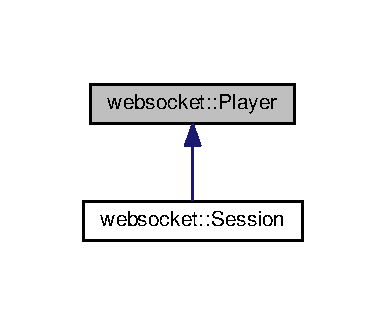
\includegraphics[width=185pt]{classwebsocket_1_1Player__inherit__graph}
\end{center}
\end{figure}
\subsection*{Public Member Functions}
\begin{DoxyCompactItemize}
\item 
virtual \hyperlink{classwebsocket_1_1Player_a3471cfad0e035a4204ff3f7e83a239f8}{$\sim$\+Player} ()
\item 
virtual void \hyperlink{classwebsocket_1_1Player_adf19a07c6497129268b3719783e7180d}{deliver} (\hyperlink{structwebsocket_1_1Dataframe}{Dataframe} msg)=0
\item 
virtual std\+::string \hyperlink{classwebsocket_1_1Player_a440338aee24d324c46115bc7b4c7a463}{get\+Id} ()=0
\end{DoxyCompactItemize}


\subsection{Constructor \& Destructor Documentation}
\index{websocket\+::\+Player@{websocket\+::\+Player}!````~Player@{$\sim$\+Player}}
\index{````~Player@{$\sim$\+Player}!websocket\+::\+Player@{websocket\+::\+Player}}
\subsubsection[{\texorpdfstring{$\sim$\+Player()}{~Player()}}]{\setlength{\rightskip}{0pt plus 5cm}virtual websocket\+::\+Player\+::$\sim$\+Player (
\begin{DoxyParamCaption}
{}
\end{DoxyParamCaption}
)\hspace{0.3cm}{\ttfamily [inline]}, {\ttfamily [virtual]}}\hypertarget{classwebsocket_1_1Player_a3471cfad0e035a4204ff3f7e83a239f8}{}\label{classwebsocket_1_1Player_a3471cfad0e035a4204ff3f7e83a239f8}


\subsection{Member Function Documentation}
\index{websocket\+::\+Player@{websocket\+::\+Player}!deliver@{deliver}}
\index{deliver@{deliver}!websocket\+::\+Player@{websocket\+::\+Player}}
\subsubsection[{\texorpdfstring{deliver(\+Dataframe msg)=0}{deliver(Dataframe msg)=0}}]{\setlength{\rightskip}{0pt plus 5cm}virtual void websocket\+::\+Player\+::deliver (
\begin{DoxyParamCaption}
\item[{{\bf Dataframe}}]{msg}
\end{DoxyParamCaption}
)\hspace{0.3cm}{\ttfamily [pure virtual]}}\hypertarget{classwebsocket_1_1Player_adf19a07c6497129268b3719783e7180d}{}\label{classwebsocket_1_1Player_adf19a07c6497129268b3719783e7180d}


Implemented in \hyperlink{classwebsocket_1_1Session_a6af4fbb5ea959b9e079e779a887c4f27}{websocket\+::\+Session}.

\index{websocket\+::\+Player@{websocket\+::\+Player}!get\+Id@{get\+Id}}
\index{get\+Id@{get\+Id}!websocket\+::\+Player@{websocket\+::\+Player}}
\subsubsection[{\texorpdfstring{get\+Id()=0}{getId()=0}}]{\setlength{\rightskip}{0pt plus 5cm}virtual std\+::string websocket\+::\+Player\+::get\+Id (
\begin{DoxyParamCaption}
{}
\end{DoxyParamCaption}
)\hspace{0.3cm}{\ttfamily [pure virtual]}}\hypertarget{classwebsocket_1_1Player_a440338aee24d324c46115bc7b4c7a463}{}\label{classwebsocket_1_1Player_a440338aee24d324c46115bc7b4c7a463}


Implemented in \hyperlink{classwebsocket_1_1Session_a1da5647ac33cae9b350b586a25297323}{websocket\+::\+Session}.



The documentation for this class was generated from the following file\+:\begin{DoxyCompactItemize}
\item 
\hyperlink{player_8hpp}{player.\+hpp}\end{DoxyCompactItemize}

\hypertarget{structwebsocket_1_1http_1_1Reply}{}\section{websocket\+:\+:http\+:\+:Reply Struct Reference}
\label{structwebsocket_1_1http_1_1Reply}\index{websocket\+::http\+::\+Reply@{websocket\+::http\+::\+Reply}}


{\ttfamily \#include $<$reply.\+hpp$>$}

\subsection*{Public Types}
\begin{DoxyCompactItemize}
\item 
enum \hyperlink{structwebsocket_1_1http_1_1Reply_ab5757d7340f55ea26952d8a4b26ecff2}{status\+\_\+type} \{ \hyperlink{structwebsocket_1_1http_1_1Reply_ab5757d7340f55ea26952d8a4b26ecff2ac40eab39089a623f51ec73b0cf56debd}{S\+W\+I\+T\+C\+H\+I\+N\+G\+\_\+\+P\+R\+O\+T\+O\+C\+O\+LS} = 101, 
\hyperlink{structwebsocket_1_1http_1_1Reply_ab5757d7340f55ea26952d8a4b26ecff2abe7be227057261b88798008ac000a50c}{B\+A\+D\+\_\+\+R\+E\+Q\+U\+E\+ST} = 400, 
\hyperlink{structwebsocket_1_1http_1_1Reply_ab5757d7340f55ea26952d8a4b26ecff2acf5dc4f995928bbd6bd1eb5b599865a0}{I\+N\+T\+E\+R\+N\+A\+L\+\_\+\+S\+E\+R\+V\+E\+R\+\_\+\+E\+R\+R\+OR} = 500
 \}\begin{DoxyCompactList}\small\item\em The status of the \hyperlink{structwebsocket_1_1http_1_1Reply}{Reply}. \end{DoxyCompactList}
\end{DoxyCompactItemize}
\subsection*{Public Member Functions}
\begin{DoxyCompactItemize}
\item 
std\+::vector$<$ boost\+::asio\+::const\+\_\+buffer $>$ \hyperlink{structwebsocket_1_1http_1_1Reply_a69b864b3b73877e32794cff8df944485}{to\+\_\+buffers} ()
\begin{DoxyCompactList}\small\item\em Convert the \hyperlink{structwebsocket_1_1http_1_1Reply}{Reply} into a vector of buffers. \end{DoxyCompactList}\end{DoxyCompactItemize}
\subsection*{Static Public Member Functions}
\begin{DoxyCompactItemize}
\item 
static \hyperlink{structwebsocket_1_1http_1_1Reply}{Reply} \hyperlink{structwebsocket_1_1http_1_1Reply_a96b71498c73c3925edd06359da59675b}{stock\+\_\+reply} (\hyperlink{structwebsocket_1_1http_1_1Reply_ab5757d7340f55ea26952d8a4b26ecff2}{status\+\_\+type} \hyperlink{structwebsocket_1_1http_1_1Reply_afa1b8fc57be88cfc33b7788d37ae42b8}{status})
\begin{DoxyCompactList}\small\item\em Get a stock \hyperlink{structwebsocket_1_1http_1_1Reply}{Reply}. \end{DoxyCompactList}\end{DoxyCompactItemize}
\subsection*{Public Attributes}
\begin{DoxyCompactItemize}
\item 
enum \hyperlink{structwebsocket_1_1http_1_1Reply_ab5757d7340f55ea26952d8a4b26ecff2}{websocket\+::http\+::\+Reply\+::status\+\_\+type} \hyperlink{structwebsocket_1_1http_1_1Reply_afa1b8fc57be88cfc33b7788d37ae42b8}{status}
\item 
std\+::vector$<$ \hyperlink{structwebsocket_1_1http_1_1Header}{Header} $>$ \hyperlink{structwebsocket_1_1http_1_1Reply_aa88f08563abdf43f15d7ff694ffd06e2}{headers}
\begin{DoxyCompactList}\small\item\em The headers to be included in the \hyperlink{structwebsocket_1_1http_1_1Reply}{Reply}. \end{DoxyCompactList}\end{DoxyCompactItemize}


\subsection{Member Enumeration Documentation}
\index{websocket\+::http\+::\+Reply@{websocket\+::http\+::\+Reply}!status\+\_\+type@{status\+\_\+type}}
\index{status\+\_\+type@{status\+\_\+type}!websocket\+::http\+::\+Reply@{websocket\+::http\+::\+Reply}}
\subsubsection[{\texorpdfstring{status\+\_\+type}{status_type}}]{\setlength{\rightskip}{0pt plus 5cm}enum {\bf websocket\+::http\+::\+Reply\+::status\+\_\+type}}\hypertarget{structwebsocket_1_1http_1_1Reply_ab5757d7340f55ea26952d8a4b26ecff2}{}\label{structwebsocket_1_1http_1_1Reply_ab5757d7340f55ea26952d8a4b26ecff2}


The status of the \hyperlink{structwebsocket_1_1http_1_1Reply}{Reply}. 

\begin{Desc}
\item[Enumerator]\par
\begin{description}
\index{S\+W\+I\+T\+C\+H\+I\+N\+G\+\_\+\+P\+R\+O\+T\+O\+C\+O\+LS@{S\+W\+I\+T\+C\+H\+I\+N\+G\+\_\+\+P\+R\+O\+T\+O\+C\+O\+LS}!websocket\+::http\+::\+Reply@{websocket\+::http\+::\+Reply}}\index{websocket\+::http\+::\+Reply@{websocket\+::http\+::\+Reply}!S\+W\+I\+T\+C\+H\+I\+N\+G\+\_\+\+P\+R\+O\+T\+O\+C\+O\+LS@{S\+W\+I\+T\+C\+H\+I\+N\+G\+\_\+\+P\+R\+O\+T\+O\+C\+O\+LS}}\item[{\em 
S\+W\+I\+T\+C\+H\+I\+N\+G\+\_\+\+P\+R\+O\+T\+O\+C\+O\+LS\hypertarget{structwebsocket_1_1http_1_1Reply_ab5757d7340f55ea26952d8a4b26ecff2ac40eab39089a623f51ec73b0cf56debd}{}\label{structwebsocket_1_1http_1_1Reply_ab5757d7340f55ea26952d8a4b26ecff2ac40eab39089a623f51ec73b0cf56debd}
}]\index{B\+A\+D\+\_\+\+R\+E\+Q\+U\+E\+ST@{B\+A\+D\+\_\+\+R\+E\+Q\+U\+E\+ST}!websocket\+::http\+::\+Reply@{websocket\+::http\+::\+Reply}}\index{websocket\+::http\+::\+Reply@{websocket\+::http\+::\+Reply}!B\+A\+D\+\_\+\+R\+E\+Q\+U\+E\+ST@{B\+A\+D\+\_\+\+R\+E\+Q\+U\+E\+ST}}\item[{\em 
B\+A\+D\+\_\+\+R\+E\+Q\+U\+E\+ST\hypertarget{structwebsocket_1_1http_1_1Reply_ab5757d7340f55ea26952d8a4b26ecff2abe7be227057261b88798008ac000a50c}{}\label{structwebsocket_1_1http_1_1Reply_ab5757d7340f55ea26952d8a4b26ecff2abe7be227057261b88798008ac000a50c}
}]\index{I\+N\+T\+E\+R\+N\+A\+L\+\_\+\+S\+E\+R\+V\+E\+R\+\_\+\+E\+R\+R\+OR@{I\+N\+T\+E\+R\+N\+A\+L\+\_\+\+S\+E\+R\+V\+E\+R\+\_\+\+E\+R\+R\+OR}!websocket\+::http\+::\+Reply@{websocket\+::http\+::\+Reply}}\index{websocket\+::http\+::\+Reply@{websocket\+::http\+::\+Reply}!I\+N\+T\+E\+R\+N\+A\+L\+\_\+\+S\+E\+R\+V\+E\+R\+\_\+\+E\+R\+R\+OR@{I\+N\+T\+E\+R\+N\+A\+L\+\_\+\+S\+E\+R\+V\+E\+R\+\_\+\+E\+R\+R\+OR}}\item[{\em 
I\+N\+T\+E\+R\+N\+A\+L\+\_\+\+S\+E\+R\+V\+E\+R\+\_\+\+E\+R\+R\+OR\hypertarget{structwebsocket_1_1http_1_1Reply_ab5757d7340f55ea26952d8a4b26ecff2acf5dc4f995928bbd6bd1eb5b599865a0}{}\label{structwebsocket_1_1http_1_1Reply_ab5757d7340f55ea26952d8a4b26ecff2acf5dc4f995928bbd6bd1eb5b599865a0}
}]\end{description}
\end{Desc}

\begin{DoxyCode}
20             \{
21                 \hyperlink{structwebsocket_1_1http_1_1Reply_ab5757d7340f55ea26952d8a4b26ecff2ac40eab39089a623f51ec73b0cf56debd}{SWITCHING\_PROTOCOLS} = 101,
22                 \hyperlink{structwebsocket_1_1http_1_1Reply_ab5757d7340f55ea26952d8a4b26ecff2abe7be227057261b88798008ac000a50c}{BAD\_REQUEST} = 400,
23                 \hyperlink{structwebsocket_1_1http_1_1Reply_ab5757d7340f55ea26952d8a4b26ecff2acf5dc4f995928bbd6bd1eb5b599865a0}{INTERNAL\_SERVER\_ERROR} = 500
24             \} \hyperlink{structwebsocket_1_1http_1_1Reply_afa1b8fc57be88cfc33b7788d37ae42b8}{status};
\end{DoxyCode}


\subsection{Member Function Documentation}
\index{websocket\+::http\+::\+Reply@{websocket\+::http\+::\+Reply}!stock\+\_\+reply@{stock\+\_\+reply}}
\index{stock\+\_\+reply@{stock\+\_\+reply}!websocket\+::http\+::\+Reply@{websocket\+::http\+::\+Reply}}
\subsubsection[{\texorpdfstring{stock\+\_\+reply(status\+\_\+type status)}{stock_reply(status_type status)}}]{\setlength{\rightskip}{0pt plus 5cm}{\bf Reply} websocket\+::http\+::\+Reply\+::stock\+\_\+reply (
\begin{DoxyParamCaption}
\item[{{\bf Reply\+::status\+\_\+type}}]{status}
\end{DoxyParamCaption}
)\hspace{0.3cm}{\ttfamily [static]}}\hypertarget{structwebsocket_1_1http_1_1Reply_a96b71498c73c3925edd06359da59675b}{}\label{structwebsocket_1_1http_1_1Reply_a96b71498c73c3925edd06359da59675b}


Get a stock \hyperlink{structwebsocket_1_1http_1_1Reply}{Reply}. 


\begin{DoxyCode}
58         \{
59             Reply rep;
60             rep.status = \hyperlink{structwebsocket_1_1http_1_1Reply_afa1b8fc57be88cfc33b7788d37ae42b8}{status};
61 
62             \textcolor{keywordflow}{return} rep;
63         \}
\end{DoxyCode}
\index{websocket\+::http\+::\+Reply@{websocket\+::http\+::\+Reply}!to\+\_\+buffers@{to\+\_\+buffers}}
\index{to\+\_\+buffers@{to\+\_\+buffers}!websocket\+::http\+::\+Reply@{websocket\+::http\+::\+Reply}}
\subsubsection[{\texorpdfstring{to\+\_\+buffers()}{to_buffers()}}]{\setlength{\rightskip}{0pt plus 5cm}std\+::vector$<$ boost\+::asio\+::const\+\_\+buffer $>$ websocket\+::http\+::\+Reply\+::to\+\_\+buffers (
\begin{DoxyParamCaption}
{}
\end{DoxyParamCaption}
)}\hypertarget{structwebsocket_1_1http_1_1Reply_a69b864b3b73877e32794cff8df944485}{}\label{structwebsocket_1_1http_1_1Reply_a69b864b3b73877e32794cff8df944485}


Convert the \hyperlink{structwebsocket_1_1http_1_1Reply}{Reply} into a vector of buffers. 


\begin{DoxyCode}
39         \{
40             std::vector<boost::asio::const\_buffer> buffers;
41             buffers.push\_back(\hyperlink{namespacewebsocket_1_1http_1_1status__strings_a71a3c805bd5bbbf577264ca762da4299}{status\_strings::to\_buffer}(
      \hyperlink{structwebsocket_1_1http_1_1Reply_afa1b8fc57be88cfc33b7788d37ae42b8}{status}));
42 
43             \textcolor{keywordflow}{for} (std::size\_t i = 0; i < \hyperlink{structwebsocket_1_1http_1_1Reply_aa88f08563abdf43f15d7ff694ffd06e2}{headers}.size(); ++i)
44             \{
45                 Header& h = \hyperlink{structwebsocket_1_1http_1_1Reply_aa88f08563abdf43f15d7ff694ffd06e2}{headers}[i];
46                 buffers.push\_back(boost::asio::buffer(h.name));
47                 buffers.push\_back(boost::asio::buffer(
      \hyperlink{namespacewebsocket_1_1http_1_1misc__strings_a8fede78f1be63335d445aabd0277727e}{misc\_strings::name\_value\_separator}));
48                 buffers.push\_back(boost::asio::buffer(h.value));
49                 buffers.push\_back(boost::asio::buffer(\hyperlink{namespacewebsocket_1_1http_1_1misc__strings_a570bafe7096a0c7904f41f8d6ada54af}{misc\_strings::crlf}));
50             \}
51 
52             buffers.push\_back(boost::asio::buffer(\hyperlink{namespacewebsocket_1_1http_1_1misc__strings_a570bafe7096a0c7904f41f8d6ada54af}{misc\_strings::crlf}));
53 
54             \textcolor{keywordflow}{return} buffers;
55         \}
\end{DoxyCode}


\subsection{Member Data Documentation}
\index{websocket\+::http\+::\+Reply@{websocket\+::http\+::\+Reply}!headers@{headers}}
\index{headers@{headers}!websocket\+::http\+::\+Reply@{websocket\+::http\+::\+Reply}}
\subsubsection[{\texorpdfstring{headers}{headers}}]{\setlength{\rightskip}{0pt plus 5cm}std\+::vector$<${\bf Header}$>$ websocket\+::http\+::\+Reply\+::headers}\hypertarget{structwebsocket_1_1http_1_1Reply_aa88f08563abdf43f15d7ff694ffd06e2}{}\label{structwebsocket_1_1http_1_1Reply_aa88f08563abdf43f15d7ff694ffd06e2}


The headers to be included in the \hyperlink{structwebsocket_1_1http_1_1Reply}{Reply}. 

\index{websocket\+::http\+::\+Reply@{websocket\+::http\+::\+Reply}!status@{status}}
\index{status@{status}!websocket\+::http\+::\+Reply@{websocket\+::http\+::\+Reply}}
\subsubsection[{\texorpdfstring{status}{status}}]{\setlength{\rightskip}{0pt plus 5cm}enum {\bf websocket\+::http\+::\+Reply\+::status\+\_\+type}  websocket\+::http\+::\+Reply\+::status}\hypertarget{structwebsocket_1_1http_1_1Reply_afa1b8fc57be88cfc33b7788d37ae42b8}{}\label{structwebsocket_1_1http_1_1Reply_afa1b8fc57be88cfc33b7788d37ae42b8}


The documentation for this struct was generated from the following files\+:\begin{DoxyCompactItemize}
\item 
\hyperlink{reply_8hpp}{reply.\+hpp}\item 
\hyperlink{reply_8cpp}{reply.\+cpp}\end{DoxyCompactItemize}

\hypertarget{structwebsocket_1_1http_1_1Request}{}\section{websocket\+:\+:http\+:\+:Request Struct Reference}
\label{structwebsocket_1_1http_1_1Request}\index{websocket\+::http\+::\+Request@{websocket\+::http\+::\+Request}}


{\ttfamily \#include $<$request.\+hpp$>$}

\subsection*{Public Attributes}
\begin{DoxyCompactItemize}
\item 
std\+::string \hyperlink{structwebsocket_1_1http_1_1Request_a698538be27d0b18b59c5caf1a0e3d495}{method}
\item 
std\+::string \hyperlink{structwebsocket_1_1http_1_1Request_a32fdc3e7be509b14c80a069dfbcf3b86}{uri}
\item 
int \hyperlink{structwebsocket_1_1http_1_1Request_a425abfd24de736ada49b1ac904316fa8}{http\+\_\+version\+\_\+major}
\item 
int \hyperlink{structwebsocket_1_1http_1_1Request_adc822c62d63286a9127d04d7d890148b}{http\+\_\+version\+\_\+minor}
\item 
std\+::vector$<$ \hyperlink{structwebsocket_1_1http_1_1Header}{Header} $>$ \hyperlink{structwebsocket_1_1http_1_1Request_a535de60f064cc2ff1a2ae5cce352b9d8}{headers}
\end{DoxyCompactItemize}


\subsection{Member Data Documentation}
\index{websocket\+::http\+::\+Request@{websocket\+::http\+::\+Request}!headers@{headers}}
\index{headers@{headers}!websocket\+::http\+::\+Request@{websocket\+::http\+::\+Request}}
\subsubsection[{\texorpdfstring{headers}{headers}}]{\setlength{\rightskip}{0pt plus 5cm}std\+::vector$<${\bf Header}$>$ websocket\+::http\+::\+Request\+::headers}\hypertarget{structwebsocket_1_1http_1_1Request_a535de60f064cc2ff1a2ae5cce352b9d8}{}\label{structwebsocket_1_1http_1_1Request_a535de60f064cc2ff1a2ae5cce352b9d8}
\index{websocket\+::http\+::\+Request@{websocket\+::http\+::\+Request}!http\+\_\+version\+\_\+major@{http\+\_\+version\+\_\+major}}
\index{http\+\_\+version\+\_\+major@{http\+\_\+version\+\_\+major}!websocket\+::http\+::\+Request@{websocket\+::http\+::\+Request}}
\subsubsection[{\texorpdfstring{http\+\_\+version\+\_\+major}{http_version_major}}]{\setlength{\rightskip}{0pt plus 5cm}int websocket\+::http\+::\+Request\+::http\+\_\+version\+\_\+major}\hypertarget{structwebsocket_1_1http_1_1Request_a425abfd24de736ada49b1ac904316fa8}{}\label{structwebsocket_1_1http_1_1Request_a425abfd24de736ada49b1ac904316fa8}
\index{websocket\+::http\+::\+Request@{websocket\+::http\+::\+Request}!http\+\_\+version\+\_\+minor@{http\+\_\+version\+\_\+minor}}
\index{http\+\_\+version\+\_\+minor@{http\+\_\+version\+\_\+minor}!websocket\+::http\+::\+Request@{websocket\+::http\+::\+Request}}
\subsubsection[{\texorpdfstring{http\+\_\+version\+\_\+minor}{http_version_minor}}]{\setlength{\rightskip}{0pt plus 5cm}int websocket\+::http\+::\+Request\+::http\+\_\+version\+\_\+minor}\hypertarget{structwebsocket_1_1http_1_1Request_adc822c62d63286a9127d04d7d890148b}{}\label{structwebsocket_1_1http_1_1Request_adc822c62d63286a9127d04d7d890148b}
\index{websocket\+::http\+::\+Request@{websocket\+::http\+::\+Request}!method@{method}}
\index{method@{method}!websocket\+::http\+::\+Request@{websocket\+::http\+::\+Request}}
\subsubsection[{\texorpdfstring{method}{method}}]{\setlength{\rightskip}{0pt plus 5cm}std\+::string websocket\+::http\+::\+Request\+::method}\hypertarget{structwebsocket_1_1http_1_1Request_a698538be27d0b18b59c5caf1a0e3d495}{}\label{structwebsocket_1_1http_1_1Request_a698538be27d0b18b59c5caf1a0e3d495}
\index{websocket\+::http\+::\+Request@{websocket\+::http\+::\+Request}!uri@{uri}}
\index{uri@{uri}!websocket\+::http\+::\+Request@{websocket\+::http\+::\+Request}}
\subsubsection[{\texorpdfstring{uri}{uri}}]{\setlength{\rightskip}{0pt plus 5cm}std\+::string websocket\+::http\+::\+Request\+::uri}\hypertarget{structwebsocket_1_1http_1_1Request_a32fdc3e7be509b14c80a069dfbcf3b86}{}\label{structwebsocket_1_1http_1_1Request_a32fdc3e7be509b14c80a069dfbcf3b86}


The documentation for this struct was generated from the following file\+:\begin{DoxyCompactItemize}
\item 
\hyperlink{request_8hpp}{request.\+hpp}\end{DoxyCompactItemize}

\hypertarget{classwebsocket_1_1http_1_1RequestHandler}{}\section{websocket\+:\+:http\+:\+:Request\+Handler Class Reference}
\label{classwebsocket_1_1http_1_1RequestHandler}\index{websocket\+::http\+::\+Request\+Handler@{websocket\+::http\+::\+Request\+Handler}}


{\ttfamily \#include $<$request\+\_\+handler.\+hpp$>$}



Inheritance diagram for websocket\+:\+:http\+:\+:Request\+Handler\+:
\nopagebreak
\begin{figure}[H]
\begin{center}
\leavevmode
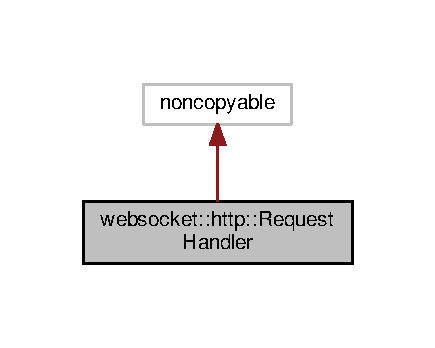
\includegraphics[width=209pt]{classwebsocket_1_1http_1_1RequestHandler__inherit__graph}
\end{center}
\end{figure}


Collaboration diagram for websocket\+:\+:http\+:\+:Request\+Handler\+:
\nopagebreak
\begin{figure}[H]
\begin{center}
\leavevmode
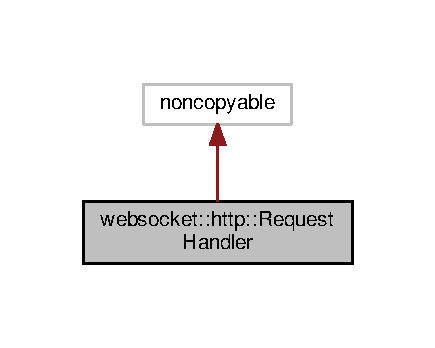
\includegraphics[width=209pt]{classwebsocket_1_1http_1_1RequestHandler__coll__graph}
\end{center}
\end{figure}
\subsection*{Static Public Member Functions}
\begin{DoxyCompactItemize}
\item 
static void \hyperlink{classwebsocket_1_1http_1_1RequestHandler_aca773bf228502c35351326f4b0dc67a9}{handle\+Request} (const \hyperlink{structwebsocket_1_1http_1_1Request}{Request} \&req, \hyperlink{structwebsocket_1_1http_1_1Reply}{Reply} \&rep)
\begin{DoxyCompactList}\small\item\em Handle a request and produce a \hyperlink{structwebsocket_1_1http_1_1Reply}{Reply}. \end{DoxyCompactList}\end{DoxyCompactItemize}
\subsection*{Static Private Member Functions}
\begin{DoxyCompactItemize}
\item 
static std\+::vector$<$ unsigned char $>$ \hyperlink{classwebsocket_1_1http_1_1RequestHandler_ab4c224809abbc4c70a4ee72a7d94639a}{to\+Sha1} (const std\+::string \&s)
\begin{DoxyCompactList}\small\item\em Encode data using the S\+H\+A1 algorithm. \end{DoxyCompactList}\item 
static std\+::string \hyperlink{classwebsocket_1_1http_1_1RequestHandler_ac685b82b354edc818177ad83574def0d}{to\+Base64} (const std\+::vector$<$ unsigned char $>$ \&data)
\begin{DoxyCompactList}\small\item\em Encode data using the Base64 algorithm. \end{DoxyCompactList}\end{DoxyCompactItemize}


\subsection{Member Function Documentation}
\index{websocket\+::http\+::\+Request\+Handler@{websocket\+::http\+::\+Request\+Handler}!handle\+Request@{handle\+Request}}
\index{handle\+Request@{handle\+Request}!websocket\+::http\+::\+Request\+Handler@{websocket\+::http\+::\+Request\+Handler}}
\subsubsection[{\texorpdfstring{handle\+Request(const Request \&req, Reply \&rep)}{handleRequest(const Request &req, Reply &rep)}}]{\setlength{\rightskip}{0pt plus 5cm}void websocket\+::http\+::\+Request\+Handler\+::handle\+Request (
\begin{DoxyParamCaption}
\item[{const {\bf Request} \&}]{req, }
\item[{{\bf Reply} \&}]{rep}
\end{DoxyParamCaption}
)\hspace{0.3cm}{\ttfamily [static]}}\hypertarget{classwebsocket_1_1http_1_1RequestHandler_aca773bf228502c35351326f4b0dc67a9}{}\label{classwebsocket_1_1http_1_1RequestHandler_aca773bf228502c35351326f4b0dc67a9}


Handle a request and produce a \hyperlink{structwebsocket_1_1http_1_1Reply}{Reply}. 

\index{websocket\+::http\+::\+Request\+Handler@{websocket\+::http\+::\+Request\+Handler}!to\+Base64@{to\+Base64}}
\index{to\+Base64@{to\+Base64}!websocket\+::http\+::\+Request\+Handler@{websocket\+::http\+::\+Request\+Handler}}
\subsubsection[{\texorpdfstring{to\+Base64(const std\+::vector$<$ unsigned char $>$ \&data)}{toBase64(const std::vector< unsigned char > &data)}}]{\setlength{\rightskip}{0pt plus 5cm}std\+::string websocket\+::http\+::\+Request\+Handler\+::to\+Base64 (
\begin{DoxyParamCaption}
\item[{const std\+::vector$<$ unsigned char $>$ \&}]{data}
\end{DoxyParamCaption}
)\hspace{0.3cm}{\ttfamily [static]}, {\ttfamily [private]}}\hypertarget{classwebsocket_1_1http_1_1RequestHandler_ac685b82b354edc818177ad83574def0d}{}\label{classwebsocket_1_1http_1_1RequestHandler_ac685b82b354edc818177ad83574def0d}


Encode data using the Base64 algorithm. 

\index{websocket\+::http\+::\+Request\+Handler@{websocket\+::http\+::\+Request\+Handler}!to\+Sha1@{to\+Sha1}}
\index{to\+Sha1@{to\+Sha1}!websocket\+::http\+::\+Request\+Handler@{websocket\+::http\+::\+Request\+Handler}}
\subsubsection[{\texorpdfstring{to\+Sha1(const std\+::string \&s)}{toSha1(const std::string &s)}}]{\setlength{\rightskip}{0pt plus 5cm}std\+::vector$<$ unsigned char $>$ websocket\+::http\+::\+Request\+Handler\+::to\+Sha1 (
\begin{DoxyParamCaption}
\item[{const std\+::string \&}]{s}
\end{DoxyParamCaption}
)\hspace{0.3cm}{\ttfamily [static]}, {\ttfamily [private]}}\hypertarget{classwebsocket_1_1http_1_1RequestHandler_ab4c224809abbc4c70a4ee72a7d94639a}{}\label{classwebsocket_1_1http_1_1RequestHandler_ab4c224809abbc4c70a4ee72a7d94639a}


Encode data using the S\+H\+A1 algorithm. 



The documentation for this class was generated from the following files\+:\begin{DoxyCompactItemize}
\item 
\hyperlink{request__handler_8hpp}{request\+\_\+handler.\+hpp}\item 
\hyperlink{request__handler_8cpp}{request\+\_\+handler.\+cpp}\end{DoxyCompactItemize}

\hypertarget{classwebsocket_1_1http_1_1RequestParser}{}\section{websocket\+:\+:http\+:\+:Request\+Parser Class Reference}
\label{classwebsocket_1_1http_1_1RequestParser}\index{websocket\+::http\+::\+Request\+Parser@{websocket\+::http\+::\+Request\+Parser}}


{\ttfamily \#include $<$request\+\_\+parser.\+hpp$>$}

\subsection*{Public Member Functions}
\begin{DoxyCompactItemize}
\item 
\hyperlink{classwebsocket_1_1http_1_1RequestParser_a0c02ad2192b73380e065c431ebaad15b}{Request\+Parser} ()
\begin{DoxyCompactList}\small\item\em Construct ready to parse the \hyperlink{structwebsocket_1_1http_1_1Request}{Request} method. \end{DoxyCompactList}\item 
void \hyperlink{classwebsocket_1_1http_1_1RequestParser_a32f5acf5850018f007a34a5357ca2dc9}{reset} ()
\begin{DoxyCompactList}\small\item\em Reset to initial parser state. \end{DoxyCompactList}\item 
{\footnotesize template$<$typename Input\+Iterator $>$ }\\boost\+::tuple$<$ boost\+::tribool, Input\+Iterator $>$ \hyperlink{classwebsocket_1_1http_1_1RequestParser_ae5dcbd6fc63f20cd9665163c6449f5a9}{parse} (\hyperlink{structwebsocket_1_1http_1_1Request}{Request} \&req, Input\+Iterator begin, Input\+Iterator end)
\begin{DoxyCompactList}\small\item\em Parse some data. \end{DoxyCompactList}\end{DoxyCompactItemize}
\subsection*{Private Types}
\begin{DoxyCompactItemize}
\item 
enum \hyperlink{classwebsocket_1_1http_1_1RequestParser_af1ad2d57d234f4ac8fb9d9656bd9c8b2}{state} \{ \\*
\hyperlink{classwebsocket_1_1http_1_1RequestParser_af1ad2d57d234f4ac8fb9d9656bd9c8b2a40f2ae25565541dc821c917c7b4e92f5}{M\+E\+T\+H\+O\+D\+\_\+\+S\+T\+A\+RT}, 
\hyperlink{classwebsocket_1_1http_1_1RequestParser_af1ad2d57d234f4ac8fb9d9656bd9c8b2a9c12697b1ce12c5888b5a1d83ab3e928}{M\+E\+T\+H\+OD}, 
\hyperlink{classwebsocket_1_1http_1_1RequestParser_af1ad2d57d234f4ac8fb9d9656bd9c8b2aa55c503336f57df5a858ceb7b2296ebf}{U\+RI}, 
\hyperlink{classwebsocket_1_1http_1_1RequestParser_af1ad2d57d234f4ac8fb9d9656bd9c8b2a665fd5e1f56202d269014a9f81b2af2d}{H\+T\+T\+P\+\_\+\+V\+E\+R\+S\+I\+O\+N\+\_\+H}, 
\\*
\hyperlink{classwebsocket_1_1http_1_1RequestParser_af1ad2d57d234f4ac8fb9d9656bd9c8b2a5dc44c05aed3d7e01d348130c1e05cc0}{H\+T\+T\+P\+\_\+\+V\+E\+R\+S\+I\+O\+N\+\_\+\+T\+\_\+1}, 
\hyperlink{classwebsocket_1_1http_1_1RequestParser_af1ad2d57d234f4ac8fb9d9656bd9c8b2a566c8cf2b02bebd48ab4774611f6475b}{H\+T\+T\+P\+\_\+\+V\+E\+R\+S\+I\+O\+N\+\_\+\+T\+\_\+2}, 
\hyperlink{classwebsocket_1_1http_1_1RequestParser_af1ad2d57d234f4ac8fb9d9656bd9c8b2aaf7b394b825c928646ad9467f9099d32}{H\+T\+T\+P\+\_\+\+V\+E\+R\+S\+I\+O\+N\+\_\+P}, 
\hyperlink{classwebsocket_1_1http_1_1RequestParser_af1ad2d57d234f4ac8fb9d9656bd9c8b2aacaa61c45cef7a30dc6e78bd596d0ca8}{H\+T\+T\+P\+\_\+\+V\+E\+R\+S\+I\+O\+N\+\_\+\+S\+L\+A\+SH}, 
\\*
\hyperlink{classwebsocket_1_1http_1_1RequestParser_af1ad2d57d234f4ac8fb9d9656bd9c8b2ade6a7fb0e6a807ae7d12884b42b54dd0}{H\+T\+T\+P\+\_\+\+V\+E\+R\+S\+I\+O\+N\+\_\+\+M\+A\+J\+O\+R\+\_\+\+S\+T\+A\+RT}, 
\hyperlink{classwebsocket_1_1http_1_1RequestParser_af1ad2d57d234f4ac8fb9d9656bd9c8b2abf76daa842c3a7b2e15a7795ae80f3ea}{H\+T\+T\+P\+\_\+\+V\+E\+R\+S\+I\+O\+N\+\_\+\+M\+A\+J\+OR}, 
\hyperlink{classwebsocket_1_1http_1_1RequestParser_af1ad2d57d234f4ac8fb9d9656bd9c8b2a514b190a9eb5c1c125b21b15ac7cb889}{H\+T\+T\+P\+\_\+\+V\+E\+R\+S\+I\+O\+N\+\_\+\+M\+I\+N\+O\+R\+\_\+\+S\+T\+A\+RT}, 
\hyperlink{classwebsocket_1_1http_1_1RequestParser_af1ad2d57d234f4ac8fb9d9656bd9c8b2ad10be8cf254e2b7f9cc5122a491526b7}{H\+T\+T\+P\+\_\+\+V\+E\+R\+S\+I\+O\+N\+\_\+\+M\+I\+N\+OR}, 
\\*
\hyperlink{classwebsocket_1_1http_1_1RequestParser_af1ad2d57d234f4ac8fb9d9656bd9c8b2a0ecb8fa46bfea7771c71c58f41268bf0}{E\+X\+P\+E\+C\+T\+I\+N\+G\+\_\+\+N\+E\+W\+L\+I\+N\+E\+\_\+1}, 
\hyperlink{classwebsocket_1_1http_1_1RequestParser_af1ad2d57d234f4ac8fb9d9656bd9c8b2aaea516ce1ac4d13a17fd513eef0ce3e1}{H\+E\+A\+D\+E\+R\+\_\+\+L\+I\+N\+E\+\_\+\+S\+T\+A\+RT}, 
\hyperlink{classwebsocket_1_1http_1_1RequestParser_af1ad2d57d234f4ac8fb9d9656bd9c8b2afc5f5b7a38b8f357143b95e9dff55981}{H\+E\+A\+D\+E\+R\+\_\+\+L\+WS}, 
\hyperlink{classwebsocket_1_1http_1_1RequestParser_af1ad2d57d234f4ac8fb9d9656bd9c8b2ab658ce46b6c2c18e7f22cbdc288124a4}{H\+E\+A\+D\+E\+R\+\_\+\+N\+A\+ME}, 
\\*
\hyperlink{classwebsocket_1_1http_1_1RequestParser_af1ad2d57d234f4ac8fb9d9656bd9c8b2a7d96b53f34b2f5734fc4219312e08303}{S\+P\+A\+C\+E\+\_\+\+B\+E\+F\+O\+R\+E\+\_\+\+H\+E\+A\+D\+E\+R\+\_\+\+V\+A\+L\+UE}, 
\hyperlink{classwebsocket_1_1http_1_1RequestParser_af1ad2d57d234f4ac8fb9d9656bd9c8b2a834d3f769b7d8f936e1db3ff09311580}{H\+E\+A\+D\+E\+R\+\_\+\+V\+A\+L\+UE}, 
\hyperlink{classwebsocket_1_1http_1_1RequestParser_af1ad2d57d234f4ac8fb9d9656bd9c8b2a382a9876ff19c807c19ca3d81d379f74}{E\+X\+P\+E\+C\+T\+I\+N\+G\+\_\+\+N\+E\+W\+L\+I\+N\+E\+\_\+2}, 
\hyperlink{classwebsocket_1_1http_1_1RequestParser_af1ad2d57d234f4ac8fb9d9656bd9c8b2ab3f9a5a7482ec9b941a93ad9490b1b24}{E\+X\+P\+E\+C\+T\+I\+N\+G\+\_\+\+N\+E\+W\+L\+I\+N\+E\+\_\+3}
 \}\begin{DoxyCompactList}\small\item\em The current state of the parser. \end{DoxyCompactList}
\end{DoxyCompactItemize}
\subsection*{Private Member Functions}
\begin{DoxyCompactItemize}
\item 
boost\+::tribool \hyperlink{classwebsocket_1_1http_1_1RequestParser_acb68b2ddadf42677684af022d2eab05a}{consume} (\hyperlink{structwebsocket_1_1http_1_1Request}{Request} \&req, char input)
\begin{DoxyCompactList}\small\item\em Handle the next character of input. \end{DoxyCompactList}\end{DoxyCompactItemize}
\subsection*{Static Private Member Functions}
\begin{DoxyCompactItemize}
\item 
static bool \hyperlink{classwebsocket_1_1http_1_1RequestParser_a3b64b2e4a7993ed710006539db861db9}{is\+\_\+char} (int c)
\begin{DoxyCompactList}\small\item\em Check if a byte is an H\+T\+TP character. \end{DoxyCompactList}\item 
static bool \hyperlink{classwebsocket_1_1http_1_1RequestParser_a7a75bf40bc4b9de6298e3e0e1d2860c2}{is\+\_\+ctl} (int c)
\begin{DoxyCompactList}\small\item\em Check if a byte is an H\+T\+TP control character. \end{DoxyCompactList}\item 
static bool \hyperlink{classwebsocket_1_1http_1_1RequestParser_aab25fc5fbe25d6eed0cc55e00ccb2fc3}{is\+\_\+tspecial} (int c)
\begin{DoxyCompactList}\small\item\em Check if a byte is defined as an H\+T\+TP tspecial character. \end{DoxyCompactList}\item 
static bool \hyperlink{classwebsocket_1_1http_1_1RequestParser_a8650b0f4d250cc7eba88666aa919b1f7}{is\+\_\+digit} (int c)
\begin{DoxyCompactList}\small\item\em Check if a byte is a digit. \end{DoxyCompactList}\end{DoxyCompactItemize}
\subsection*{Private Attributes}
\begin{DoxyCompactItemize}
\item 
enum \hyperlink{classwebsocket_1_1http_1_1RequestParser_af1ad2d57d234f4ac8fb9d9656bd9c8b2}{websocket\+::http\+::\+Request\+Parser\+::state} \hyperlink{classwebsocket_1_1http_1_1RequestParser_aed48589d041848aabcd27672a0a4ad73}{state\+\_\+}
\end{DoxyCompactItemize}


\subsection{Member Enumeration Documentation}
\index{websocket\+::http\+::\+Request\+Parser@{websocket\+::http\+::\+Request\+Parser}!state@{state}}
\index{state@{state}!websocket\+::http\+::\+Request\+Parser@{websocket\+::http\+::\+Request\+Parser}}
\subsubsection[{\texorpdfstring{state}{state}}]{\setlength{\rightskip}{0pt plus 5cm}enum {\bf websocket\+::http\+::\+Request\+Parser\+::state}\hspace{0.3cm}{\ttfamily [private]}}\hypertarget{classwebsocket_1_1http_1_1RequestParser_af1ad2d57d234f4ac8fb9d9656bd9c8b2}{}\label{classwebsocket_1_1http_1_1RequestParser_af1ad2d57d234f4ac8fb9d9656bd9c8b2}


The current state of the parser. 

\begin{Desc}
\item[Enumerator]\par
\begin{description}
\index{M\+E\+T\+H\+O\+D\+\_\+\+S\+T\+A\+RT@{M\+E\+T\+H\+O\+D\+\_\+\+S\+T\+A\+RT}!websocket\+::http\+::\+Request\+Parser@{websocket\+::http\+::\+Request\+Parser}}\index{websocket\+::http\+::\+Request\+Parser@{websocket\+::http\+::\+Request\+Parser}!M\+E\+T\+H\+O\+D\+\_\+\+S\+T\+A\+RT@{M\+E\+T\+H\+O\+D\+\_\+\+S\+T\+A\+RT}}\item[{\em 
M\+E\+T\+H\+O\+D\+\_\+\+S\+T\+A\+RT\hypertarget{classwebsocket_1_1http_1_1RequestParser_af1ad2d57d234f4ac8fb9d9656bd9c8b2a40f2ae25565541dc821c917c7b4e92f5}{}\label{classwebsocket_1_1http_1_1RequestParser_af1ad2d57d234f4ac8fb9d9656bd9c8b2a40f2ae25565541dc821c917c7b4e92f5}
}]\index{M\+E\+T\+H\+OD@{M\+E\+T\+H\+OD}!websocket\+::http\+::\+Request\+Parser@{websocket\+::http\+::\+Request\+Parser}}\index{websocket\+::http\+::\+Request\+Parser@{websocket\+::http\+::\+Request\+Parser}!M\+E\+T\+H\+OD@{M\+E\+T\+H\+OD}}\item[{\em 
M\+E\+T\+H\+OD\hypertarget{classwebsocket_1_1http_1_1RequestParser_af1ad2d57d234f4ac8fb9d9656bd9c8b2a9c12697b1ce12c5888b5a1d83ab3e928}{}\label{classwebsocket_1_1http_1_1RequestParser_af1ad2d57d234f4ac8fb9d9656bd9c8b2a9c12697b1ce12c5888b5a1d83ab3e928}
}]\index{U\+RI@{U\+RI}!websocket\+::http\+::\+Request\+Parser@{websocket\+::http\+::\+Request\+Parser}}\index{websocket\+::http\+::\+Request\+Parser@{websocket\+::http\+::\+Request\+Parser}!U\+RI@{U\+RI}}\item[{\em 
U\+RI\hypertarget{classwebsocket_1_1http_1_1RequestParser_af1ad2d57d234f4ac8fb9d9656bd9c8b2aa55c503336f57df5a858ceb7b2296ebf}{}\label{classwebsocket_1_1http_1_1RequestParser_af1ad2d57d234f4ac8fb9d9656bd9c8b2aa55c503336f57df5a858ceb7b2296ebf}
}]\index{H\+T\+T\+P\+\_\+\+V\+E\+R\+S\+I\+O\+N\+\_\+H@{H\+T\+T\+P\+\_\+\+V\+E\+R\+S\+I\+O\+N\+\_\+H}!websocket\+::http\+::\+Request\+Parser@{websocket\+::http\+::\+Request\+Parser}}\index{websocket\+::http\+::\+Request\+Parser@{websocket\+::http\+::\+Request\+Parser}!H\+T\+T\+P\+\_\+\+V\+E\+R\+S\+I\+O\+N\+\_\+H@{H\+T\+T\+P\+\_\+\+V\+E\+R\+S\+I\+O\+N\+\_\+H}}\item[{\em 
H\+T\+T\+P\+\_\+\+V\+E\+R\+S\+I\+O\+N\+\_\+H\hypertarget{classwebsocket_1_1http_1_1RequestParser_af1ad2d57d234f4ac8fb9d9656bd9c8b2a665fd5e1f56202d269014a9f81b2af2d}{}\label{classwebsocket_1_1http_1_1RequestParser_af1ad2d57d234f4ac8fb9d9656bd9c8b2a665fd5e1f56202d269014a9f81b2af2d}
}]\index{H\+T\+T\+P\+\_\+\+V\+E\+R\+S\+I\+O\+N\+\_\+\+T\+\_\+1@{H\+T\+T\+P\+\_\+\+V\+E\+R\+S\+I\+O\+N\+\_\+\+T\+\_\+1}!websocket\+::http\+::\+Request\+Parser@{websocket\+::http\+::\+Request\+Parser}}\index{websocket\+::http\+::\+Request\+Parser@{websocket\+::http\+::\+Request\+Parser}!H\+T\+T\+P\+\_\+\+V\+E\+R\+S\+I\+O\+N\+\_\+\+T\+\_\+1@{H\+T\+T\+P\+\_\+\+V\+E\+R\+S\+I\+O\+N\+\_\+\+T\+\_\+1}}\item[{\em 
H\+T\+T\+P\+\_\+\+V\+E\+R\+S\+I\+O\+N\+\_\+\+T\+\_\+1\hypertarget{classwebsocket_1_1http_1_1RequestParser_af1ad2d57d234f4ac8fb9d9656bd9c8b2a5dc44c05aed3d7e01d348130c1e05cc0}{}\label{classwebsocket_1_1http_1_1RequestParser_af1ad2d57d234f4ac8fb9d9656bd9c8b2a5dc44c05aed3d7e01d348130c1e05cc0}
}]\index{H\+T\+T\+P\+\_\+\+V\+E\+R\+S\+I\+O\+N\+\_\+\+T\+\_\+2@{H\+T\+T\+P\+\_\+\+V\+E\+R\+S\+I\+O\+N\+\_\+\+T\+\_\+2}!websocket\+::http\+::\+Request\+Parser@{websocket\+::http\+::\+Request\+Parser}}\index{websocket\+::http\+::\+Request\+Parser@{websocket\+::http\+::\+Request\+Parser}!H\+T\+T\+P\+\_\+\+V\+E\+R\+S\+I\+O\+N\+\_\+\+T\+\_\+2@{H\+T\+T\+P\+\_\+\+V\+E\+R\+S\+I\+O\+N\+\_\+\+T\+\_\+2}}\item[{\em 
H\+T\+T\+P\+\_\+\+V\+E\+R\+S\+I\+O\+N\+\_\+\+T\+\_\+2\hypertarget{classwebsocket_1_1http_1_1RequestParser_af1ad2d57d234f4ac8fb9d9656bd9c8b2a566c8cf2b02bebd48ab4774611f6475b}{}\label{classwebsocket_1_1http_1_1RequestParser_af1ad2d57d234f4ac8fb9d9656bd9c8b2a566c8cf2b02bebd48ab4774611f6475b}
}]\index{H\+T\+T\+P\+\_\+\+V\+E\+R\+S\+I\+O\+N\+\_\+P@{H\+T\+T\+P\+\_\+\+V\+E\+R\+S\+I\+O\+N\+\_\+P}!websocket\+::http\+::\+Request\+Parser@{websocket\+::http\+::\+Request\+Parser}}\index{websocket\+::http\+::\+Request\+Parser@{websocket\+::http\+::\+Request\+Parser}!H\+T\+T\+P\+\_\+\+V\+E\+R\+S\+I\+O\+N\+\_\+P@{H\+T\+T\+P\+\_\+\+V\+E\+R\+S\+I\+O\+N\+\_\+P}}\item[{\em 
H\+T\+T\+P\+\_\+\+V\+E\+R\+S\+I\+O\+N\+\_\+P\hypertarget{classwebsocket_1_1http_1_1RequestParser_af1ad2d57d234f4ac8fb9d9656bd9c8b2aaf7b394b825c928646ad9467f9099d32}{}\label{classwebsocket_1_1http_1_1RequestParser_af1ad2d57d234f4ac8fb9d9656bd9c8b2aaf7b394b825c928646ad9467f9099d32}
}]\index{H\+T\+T\+P\+\_\+\+V\+E\+R\+S\+I\+O\+N\+\_\+\+S\+L\+A\+SH@{H\+T\+T\+P\+\_\+\+V\+E\+R\+S\+I\+O\+N\+\_\+\+S\+L\+A\+SH}!websocket\+::http\+::\+Request\+Parser@{websocket\+::http\+::\+Request\+Parser}}\index{websocket\+::http\+::\+Request\+Parser@{websocket\+::http\+::\+Request\+Parser}!H\+T\+T\+P\+\_\+\+V\+E\+R\+S\+I\+O\+N\+\_\+\+S\+L\+A\+SH@{H\+T\+T\+P\+\_\+\+V\+E\+R\+S\+I\+O\+N\+\_\+\+S\+L\+A\+SH}}\item[{\em 
H\+T\+T\+P\+\_\+\+V\+E\+R\+S\+I\+O\+N\+\_\+\+S\+L\+A\+SH\hypertarget{classwebsocket_1_1http_1_1RequestParser_af1ad2d57d234f4ac8fb9d9656bd9c8b2aacaa61c45cef7a30dc6e78bd596d0ca8}{}\label{classwebsocket_1_1http_1_1RequestParser_af1ad2d57d234f4ac8fb9d9656bd9c8b2aacaa61c45cef7a30dc6e78bd596d0ca8}
}]\index{H\+T\+T\+P\+\_\+\+V\+E\+R\+S\+I\+O\+N\+\_\+\+M\+A\+J\+O\+R\+\_\+\+S\+T\+A\+RT@{H\+T\+T\+P\+\_\+\+V\+E\+R\+S\+I\+O\+N\+\_\+\+M\+A\+J\+O\+R\+\_\+\+S\+T\+A\+RT}!websocket\+::http\+::\+Request\+Parser@{websocket\+::http\+::\+Request\+Parser}}\index{websocket\+::http\+::\+Request\+Parser@{websocket\+::http\+::\+Request\+Parser}!H\+T\+T\+P\+\_\+\+V\+E\+R\+S\+I\+O\+N\+\_\+\+M\+A\+J\+O\+R\+\_\+\+S\+T\+A\+RT@{H\+T\+T\+P\+\_\+\+V\+E\+R\+S\+I\+O\+N\+\_\+\+M\+A\+J\+O\+R\+\_\+\+S\+T\+A\+RT}}\item[{\em 
H\+T\+T\+P\+\_\+\+V\+E\+R\+S\+I\+O\+N\+\_\+\+M\+A\+J\+O\+R\+\_\+\+S\+T\+A\+RT\hypertarget{classwebsocket_1_1http_1_1RequestParser_af1ad2d57d234f4ac8fb9d9656bd9c8b2ade6a7fb0e6a807ae7d12884b42b54dd0}{}\label{classwebsocket_1_1http_1_1RequestParser_af1ad2d57d234f4ac8fb9d9656bd9c8b2ade6a7fb0e6a807ae7d12884b42b54dd0}
}]\index{H\+T\+T\+P\+\_\+\+V\+E\+R\+S\+I\+O\+N\+\_\+\+M\+A\+J\+OR@{H\+T\+T\+P\+\_\+\+V\+E\+R\+S\+I\+O\+N\+\_\+\+M\+A\+J\+OR}!websocket\+::http\+::\+Request\+Parser@{websocket\+::http\+::\+Request\+Parser}}\index{websocket\+::http\+::\+Request\+Parser@{websocket\+::http\+::\+Request\+Parser}!H\+T\+T\+P\+\_\+\+V\+E\+R\+S\+I\+O\+N\+\_\+\+M\+A\+J\+OR@{H\+T\+T\+P\+\_\+\+V\+E\+R\+S\+I\+O\+N\+\_\+\+M\+A\+J\+OR}}\item[{\em 
H\+T\+T\+P\+\_\+\+V\+E\+R\+S\+I\+O\+N\+\_\+\+M\+A\+J\+OR\hypertarget{classwebsocket_1_1http_1_1RequestParser_af1ad2d57d234f4ac8fb9d9656bd9c8b2abf76daa842c3a7b2e15a7795ae80f3ea}{}\label{classwebsocket_1_1http_1_1RequestParser_af1ad2d57d234f4ac8fb9d9656bd9c8b2abf76daa842c3a7b2e15a7795ae80f3ea}
}]\index{H\+T\+T\+P\+\_\+\+V\+E\+R\+S\+I\+O\+N\+\_\+\+M\+I\+N\+O\+R\+\_\+\+S\+T\+A\+RT@{H\+T\+T\+P\+\_\+\+V\+E\+R\+S\+I\+O\+N\+\_\+\+M\+I\+N\+O\+R\+\_\+\+S\+T\+A\+RT}!websocket\+::http\+::\+Request\+Parser@{websocket\+::http\+::\+Request\+Parser}}\index{websocket\+::http\+::\+Request\+Parser@{websocket\+::http\+::\+Request\+Parser}!H\+T\+T\+P\+\_\+\+V\+E\+R\+S\+I\+O\+N\+\_\+\+M\+I\+N\+O\+R\+\_\+\+S\+T\+A\+RT@{H\+T\+T\+P\+\_\+\+V\+E\+R\+S\+I\+O\+N\+\_\+\+M\+I\+N\+O\+R\+\_\+\+S\+T\+A\+RT}}\item[{\em 
H\+T\+T\+P\+\_\+\+V\+E\+R\+S\+I\+O\+N\+\_\+\+M\+I\+N\+O\+R\+\_\+\+S\+T\+A\+RT\hypertarget{classwebsocket_1_1http_1_1RequestParser_af1ad2d57d234f4ac8fb9d9656bd9c8b2a514b190a9eb5c1c125b21b15ac7cb889}{}\label{classwebsocket_1_1http_1_1RequestParser_af1ad2d57d234f4ac8fb9d9656bd9c8b2a514b190a9eb5c1c125b21b15ac7cb889}
}]\index{H\+T\+T\+P\+\_\+\+V\+E\+R\+S\+I\+O\+N\+\_\+\+M\+I\+N\+OR@{H\+T\+T\+P\+\_\+\+V\+E\+R\+S\+I\+O\+N\+\_\+\+M\+I\+N\+OR}!websocket\+::http\+::\+Request\+Parser@{websocket\+::http\+::\+Request\+Parser}}\index{websocket\+::http\+::\+Request\+Parser@{websocket\+::http\+::\+Request\+Parser}!H\+T\+T\+P\+\_\+\+V\+E\+R\+S\+I\+O\+N\+\_\+\+M\+I\+N\+OR@{H\+T\+T\+P\+\_\+\+V\+E\+R\+S\+I\+O\+N\+\_\+\+M\+I\+N\+OR}}\item[{\em 
H\+T\+T\+P\+\_\+\+V\+E\+R\+S\+I\+O\+N\+\_\+\+M\+I\+N\+OR\hypertarget{classwebsocket_1_1http_1_1RequestParser_af1ad2d57d234f4ac8fb9d9656bd9c8b2ad10be8cf254e2b7f9cc5122a491526b7}{}\label{classwebsocket_1_1http_1_1RequestParser_af1ad2d57d234f4ac8fb9d9656bd9c8b2ad10be8cf254e2b7f9cc5122a491526b7}
}]\index{E\+X\+P\+E\+C\+T\+I\+N\+G\+\_\+\+N\+E\+W\+L\+I\+N\+E\+\_\+1@{E\+X\+P\+E\+C\+T\+I\+N\+G\+\_\+\+N\+E\+W\+L\+I\+N\+E\+\_\+1}!websocket\+::http\+::\+Request\+Parser@{websocket\+::http\+::\+Request\+Parser}}\index{websocket\+::http\+::\+Request\+Parser@{websocket\+::http\+::\+Request\+Parser}!E\+X\+P\+E\+C\+T\+I\+N\+G\+\_\+\+N\+E\+W\+L\+I\+N\+E\+\_\+1@{E\+X\+P\+E\+C\+T\+I\+N\+G\+\_\+\+N\+E\+W\+L\+I\+N\+E\+\_\+1}}\item[{\em 
E\+X\+P\+E\+C\+T\+I\+N\+G\+\_\+\+N\+E\+W\+L\+I\+N\+E\+\_\+1\hypertarget{classwebsocket_1_1http_1_1RequestParser_af1ad2d57d234f4ac8fb9d9656bd9c8b2a0ecb8fa46bfea7771c71c58f41268bf0}{}\label{classwebsocket_1_1http_1_1RequestParser_af1ad2d57d234f4ac8fb9d9656bd9c8b2a0ecb8fa46bfea7771c71c58f41268bf0}
}]\index{H\+E\+A\+D\+E\+R\+\_\+\+L\+I\+N\+E\+\_\+\+S\+T\+A\+RT@{H\+E\+A\+D\+E\+R\+\_\+\+L\+I\+N\+E\+\_\+\+S\+T\+A\+RT}!websocket\+::http\+::\+Request\+Parser@{websocket\+::http\+::\+Request\+Parser}}\index{websocket\+::http\+::\+Request\+Parser@{websocket\+::http\+::\+Request\+Parser}!H\+E\+A\+D\+E\+R\+\_\+\+L\+I\+N\+E\+\_\+\+S\+T\+A\+RT@{H\+E\+A\+D\+E\+R\+\_\+\+L\+I\+N\+E\+\_\+\+S\+T\+A\+RT}}\item[{\em 
H\+E\+A\+D\+E\+R\+\_\+\+L\+I\+N\+E\+\_\+\+S\+T\+A\+RT\hypertarget{classwebsocket_1_1http_1_1RequestParser_af1ad2d57d234f4ac8fb9d9656bd9c8b2aaea516ce1ac4d13a17fd513eef0ce3e1}{}\label{classwebsocket_1_1http_1_1RequestParser_af1ad2d57d234f4ac8fb9d9656bd9c8b2aaea516ce1ac4d13a17fd513eef0ce3e1}
}]\index{H\+E\+A\+D\+E\+R\+\_\+\+L\+WS@{H\+E\+A\+D\+E\+R\+\_\+\+L\+WS}!websocket\+::http\+::\+Request\+Parser@{websocket\+::http\+::\+Request\+Parser}}\index{websocket\+::http\+::\+Request\+Parser@{websocket\+::http\+::\+Request\+Parser}!H\+E\+A\+D\+E\+R\+\_\+\+L\+WS@{H\+E\+A\+D\+E\+R\+\_\+\+L\+WS}}\item[{\em 
H\+E\+A\+D\+E\+R\+\_\+\+L\+WS\hypertarget{classwebsocket_1_1http_1_1RequestParser_af1ad2d57d234f4ac8fb9d9656bd9c8b2afc5f5b7a38b8f357143b95e9dff55981}{}\label{classwebsocket_1_1http_1_1RequestParser_af1ad2d57d234f4ac8fb9d9656bd9c8b2afc5f5b7a38b8f357143b95e9dff55981}
}]\index{H\+E\+A\+D\+E\+R\+\_\+\+N\+A\+ME@{H\+E\+A\+D\+E\+R\+\_\+\+N\+A\+ME}!websocket\+::http\+::\+Request\+Parser@{websocket\+::http\+::\+Request\+Parser}}\index{websocket\+::http\+::\+Request\+Parser@{websocket\+::http\+::\+Request\+Parser}!H\+E\+A\+D\+E\+R\+\_\+\+N\+A\+ME@{H\+E\+A\+D\+E\+R\+\_\+\+N\+A\+ME}}\item[{\em 
H\+E\+A\+D\+E\+R\+\_\+\+N\+A\+ME\hypertarget{classwebsocket_1_1http_1_1RequestParser_af1ad2d57d234f4ac8fb9d9656bd9c8b2ab658ce46b6c2c18e7f22cbdc288124a4}{}\label{classwebsocket_1_1http_1_1RequestParser_af1ad2d57d234f4ac8fb9d9656bd9c8b2ab658ce46b6c2c18e7f22cbdc288124a4}
}]\index{S\+P\+A\+C\+E\+\_\+\+B\+E\+F\+O\+R\+E\+\_\+\+H\+E\+A\+D\+E\+R\+\_\+\+V\+A\+L\+UE@{S\+P\+A\+C\+E\+\_\+\+B\+E\+F\+O\+R\+E\+\_\+\+H\+E\+A\+D\+E\+R\+\_\+\+V\+A\+L\+UE}!websocket\+::http\+::\+Request\+Parser@{websocket\+::http\+::\+Request\+Parser}}\index{websocket\+::http\+::\+Request\+Parser@{websocket\+::http\+::\+Request\+Parser}!S\+P\+A\+C\+E\+\_\+\+B\+E\+F\+O\+R\+E\+\_\+\+H\+E\+A\+D\+E\+R\+\_\+\+V\+A\+L\+UE@{S\+P\+A\+C\+E\+\_\+\+B\+E\+F\+O\+R\+E\+\_\+\+H\+E\+A\+D\+E\+R\+\_\+\+V\+A\+L\+UE}}\item[{\em 
S\+P\+A\+C\+E\+\_\+\+B\+E\+F\+O\+R\+E\+\_\+\+H\+E\+A\+D\+E\+R\+\_\+\+V\+A\+L\+UE\hypertarget{classwebsocket_1_1http_1_1RequestParser_af1ad2d57d234f4ac8fb9d9656bd9c8b2a7d96b53f34b2f5734fc4219312e08303}{}\label{classwebsocket_1_1http_1_1RequestParser_af1ad2d57d234f4ac8fb9d9656bd9c8b2a7d96b53f34b2f5734fc4219312e08303}
}]\index{H\+E\+A\+D\+E\+R\+\_\+\+V\+A\+L\+UE@{H\+E\+A\+D\+E\+R\+\_\+\+V\+A\+L\+UE}!websocket\+::http\+::\+Request\+Parser@{websocket\+::http\+::\+Request\+Parser}}\index{websocket\+::http\+::\+Request\+Parser@{websocket\+::http\+::\+Request\+Parser}!H\+E\+A\+D\+E\+R\+\_\+\+V\+A\+L\+UE@{H\+E\+A\+D\+E\+R\+\_\+\+V\+A\+L\+UE}}\item[{\em 
H\+E\+A\+D\+E\+R\+\_\+\+V\+A\+L\+UE\hypertarget{classwebsocket_1_1http_1_1RequestParser_af1ad2d57d234f4ac8fb9d9656bd9c8b2a834d3f769b7d8f936e1db3ff09311580}{}\label{classwebsocket_1_1http_1_1RequestParser_af1ad2d57d234f4ac8fb9d9656bd9c8b2a834d3f769b7d8f936e1db3ff09311580}
}]\index{E\+X\+P\+E\+C\+T\+I\+N\+G\+\_\+\+N\+E\+W\+L\+I\+N\+E\+\_\+2@{E\+X\+P\+E\+C\+T\+I\+N\+G\+\_\+\+N\+E\+W\+L\+I\+N\+E\+\_\+2}!websocket\+::http\+::\+Request\+Parser@{websocket\+::http\+::\+Request\+Parser}}\index{websocket\+::http\+::\+Request\+Parser@{websocket\+::http\+::\+Request\+Parser}!E\+X\+P\+E\+C\+T\+I\+N\+G\+\_\+\+N\+E\+W\+L\+I\+N\+E\+\_\+2@{E\+X\+P\+E\+C\+T\+I\+N\+G\+\_\+\+N\+E\+W\+L\+I\+N\+E\+\_\+2}}\item[{\em 
E\+X\+P\+E\+C\+T\+I\+N\+G\+\_\+\+N\+E\+W\+L\+I\+N\+E\+\_\+2\hypertarget{classwebsocket_1_1http_1_1RequestParser_af1ad2d57d234f4ac8fb9d9656bd9c8b2a382a9876ff19c807c19ca3d81d379f74}{}\label{classwebsocket_1_1http_1_1RequestParser_af1ad2d57d234f4ac8fb9d9656bd9c8b2a382a9876ff19c807c19ca3d81d379f74}
}]\index{E\+X\+P\+E\+C\+T\+I\+N\+G\+\_\+\+N\+E\+W\+L\+I\+N\+E\+\_\+3@{E\+X\+P\+E\+C\+T\+I\+N\+G\+\_\+\+N\+E\+W\+L\+I\+N\+E\+\_\+3}!websocket\+::http\+::\+Request\+Parser@{websocket\+::http\+::\+Request\+Parser}}\index{websocket\+::http\+::\+Request\+Parser@{websocket\+::http\+::\+Request\+Parser}!E\+X\+P\+E\+C\+T\+I\+N\+G\+\_\+\+N\+E\+W\+L\+I\+N\+E\+\_\+3@{E\+X\+P\+E\+C\+T\+I\+N\+G\+\_\+\+N\+E\+W\+L\+I\+N\+E\+\_\+3}}\item[{\em 
E\+X\+P\+E\+C\+T\+I\+N\+G\+\_\+\+N\+E\+W\+L\+I\+N\+E\+\_\+3\hypertarget{classwebsocket_1_1http_1_1RequestParser_af1ad2d57d234f4ac8fb9d9656bd9c8b2ab3f9a5a7482ec9b941a93ad9490b1b24}{}\label{classwebsocket_1_1http_1_1RequestParser_af1ad2d57d234f4ac8fb9d9656bd9c8b2ab3f9a5a7482ec9b941a93ad9490b1b24}
}]\end{description}
\end{Desc}


\subsection{Constructor \& Destructor Documentation}
\index{websocket\+::http\+::\+Request\+Parser@{websocket\+::http\+::\+Request\+Parser}!Request\+Parser@{Request\+Parser}}
\index{Request\+Parser@{Request\+Parser}!websocket\+::http\+::\+Request\+Parser@{websocket\+::http\+::\+Request\+Parser}}
\subsubsection[{\texorpdfstring{Request\+Parser()}{RequestParser()}}]{\setlength{\rightskip}{0pt plus 5cm}websocket\+::http\+::\+Request\+Parser\+::\+Request\+Parser (
\begin{DoxyParamCaption}
{}
\end{DoxyParamCaption}
)}\hypertarget{classwebsocket_1_1http_1_1RequestParser_a0c02ad2192b73380e065c431ebaad15b}{}\label{classwebsocket_1_1http_1_1RequestParser_a0c02ad2192b73380e065c431ebaad15b}


Construct ready to parse the \hyperlink{structwebsocket_1_1http_1_1Request}{Request} method. 



\subsection{Member Function Documentation}
\index{websocket\+::http\+::\+Request\+Parser@{websocket\+::http\+::\+Request\+Parser}!consume@{consume}}
\index{consume@{consume}!websocket\+::http\+::\+Request\+Parser@{websocket\+::http\+::\+Request\+Parser}}
\subsubsection[{\texorpdfstring{consume(\+Request \&req, char input)}{consume(Request &req, char input)}}]{\setlength{\rightskip}{0pt plus 5cm}boost\+::tribool websocket\+::http\+::\+Request\+Parser\+::consume (
\begin{DoxyParamCaption}
\item[{{\bf Request} \&}]{req, }
\item[{char}]{input}
\end{DoxyParamCaption}
)\hspace{0.3cm}{\ttfamily [private]}}\hypertarget{classwebsocket_1_1http_1_1RequestParser_acb68b2ddadf42677684af022d2eab05a}{}\label{classwebsocket_1_1http_1_1RequestParser_acb68b2ddadf42677684af022d2eab05a}


Handle the next character of input. 

\index{websocket\+::http\+::\+Request\+Parser@{websocket\+::http\+::\+Request\+Parser}!is\+\_\+char@{is\+\_\+char}}
\index{is\+\_\+char@{is\+\_\+char}!websocket\+::http\+::\+Request\+Parser@{websocket\+::http\+::\+Request\+Parser}}
\subsubsection[{\texorpdfstring{is\+\_\+char(int c)}{is_char(int c)}}]{\setlength{\rightskip}{0pt plus 5cm}bool websocket\+::http\+::\+Request\+Parser\+::is\+\_\+char (
\begin{DoxyParamCaption}
\item[{int}]{c}
\end{DoxyParamCaption}
)\hspace{0.3cm}{\ttfamily [static]}, {\ttfamily [private]}}\hypertarget{classwebsocket_1_1http_1_1RequestParser_a3b64b2e4a7993ed710006539db861db9}{}\label{classwebsocket_1_1http_1_1RequestParser_a3b64b2e4a7993ed710006539db861db9}


Check if a byte is an H\+T\+TP character. 

\index{websocket\+::http\+::\+Request\+Parser@{websocket\+::http\+::\+Request\+Parser}!is\+\_\+ctl@{is\+\_\+ctl}}
\index{is\+\_\+ctl@{is\+\_\+ctl}!websocket\+::http\+::\+Request\+Parser@{websocket\+::http\+::\+Request\+Parser}}
\subsubsection[{\texorpdfstring{is\+\_\+ctl(int c)}{is_ctl(int c)}}]{\setlength{\rightskip}{0pt plus 5cm}bool websocket\+::http\+::\+Request\+Parser\+::is\+\_\+ctl (
\begin{DoxyParamCaption}
\item[{int}]{c}
\end{DoxyParamCaption}
)\hspace{0.3cm}{\ttfamily [static]}, {\ttfamily [private]}}\hypertarget{classwebsocket_1_1http_1_1RequestParser_a7a75bf40bc4b9de6298e3e0e1d2860c2}{}\label{classwebsocket_1_1http_1_1RequestParser_a7a75bf40bc4b9de6298e3e0e1d2860c2}


Check if a byte is an H\+T\+TP control character. 

\index{websocket\+::http\+::\+Request\+Parser@{websocket\+::http\+::\+Request\+Parser}!is\+\_\+digit@{is\+\_\+digit}}
\index{is\+\_\+digit@{is\+\_\+digit}!websocket\+::http\+::\+Request\+Parser@{websocket\+::http\+::\+Request\+Parser}}
\subsubsection[{\texorpdfstring{is\+\_\+digit(int c)}{is_digit(int c)}}]{\setlength{\rightskip}{0pt plus 5cm}bool websocket\+::http\+::\+Request\+Parser\+::is\+\_\+digit (
\begin{DoxyParamCaption}
\item[{int}]{c}
\end{DoxyParamCaption}
)\hspace{0.3cm}{\ttfamily [static]}, {\ttfamily [private]}}\hypertarget{classwebsocket_1_1http_1_1RequestParser_a8650b0f4d250cc7eba88666aa919b1f7}{}\label{classwebsocket_1_1http_1_1RequestParser_a8650b0f4d250cc7eba88666aa919b1f7}


Check if a byte is a digit. 

\index{websocket\+::http\+::\+Request\+Parser@{websocket\+::http\+::\+Request\+Parser}!is\+\_\+tspecial@{is\+\_\+tspecial}}
\index{is\+\_\+tspecial@{is\+\_\+tspecial}!websocket\+::http\+::\+Request\+Parser@{websocket\+::http\+::\+Request\+Parser}}
\subsubsection[{\texorpdfstring{is\+\_\+tspecial(int c)}{is_tspecial(int c)}}]{\setlength{\rightskip}{0pt plus 5cm}bool websocket\+::http\+::\+Request\+Parser\+::is\+\_\+tspecial (
\begin{DoxyParamCaption}
\item[{int}]{c}
\end{DoxyParamCaption}
)\hspace{0.3cm}{\ttfamily [static]}, {\ttfamily [private]}}\hypertarget{classwebsocket_1_1http_1_1RequestParser_aab25fc5fbe25d6eed0cc55e00ccb2fc3}{}\label{classwebsocket_1_1http_1_1RequestParser_aab25fc5fbe25d6eed0cc55e00ccb2fc3}


Check if a byte is defined as an H\+T\+TP tspecial character. 

\index{websocket\+::http\+::\+Request\+Parser@{websocket\+::http\+::\+Request\+Parser}!parse@{parse}}
\index{parse@{parse}!websocket\+::http\+::\+Request\+Parser@{websocket\+::http\+::\+Request\+Parser}}
\subsubsection[{\texorpdfstring{parse(\+Request \&req, Input\+Iterator begin, Input\+Iterator end)}{parse(Request &req, InputIterator begin, InputIterator end)}}]{\setlength{\rightskip}{0pt plus 5cm}template$<$typename Input\+Iterator $>$ boost\+::tuple$<$boost\+::tribool, Input\+Iterator$>$ websocket\+::http\+::\+Request\+Parser\+::parse (
\begin{DoxyParamCaption}
\item[{{\bf Request} \&}]{req, }
\item[{Input\+Iterator}]{begin, }
\item[{Input\+Iterator}]{end}
\end{DoxyParamCaption}
)\hspace{0.3cm}{\ttfamily [inline]}}\hypertarget{classwebsocket_1_1http_1_1RequestParser_ae5dcbd6fc63f20cd9665163c6449f5a9}{}\label{classwebsocket_1_1http_1_1RequestParser_ae5dcbd6fc63f20cd9665163c6449f5a9}


Parse some data. 

\index{websocket\+::http\+::\+Request\+Parser@{websocket\+::http\+::\+Request\+Parser}!reset@{reset}}
\index{reset@{reset}!websocket\+::http\+::\+Request\+Parser@{websocket\+::http\+::\+Request\+Parser}}
\subsubsection[{\texorpdfstring{reset()}{reset()}}]{\setlength{\rightskip}{0pt plus 5cm}void websocket\+::http\+::\+Request\+Parser\+::reset (
\begin{DoxyParamCaption}
{}
\end{DoxyParamCaption}
)}\hypertarget{classwebsocket_1_1http_1_1RequestParser_a32f5acf5850018f007a34a5357ca2dc9}{}\label{classwebsocket_1_1http_1_1RequestParser_a32f5acf5850018f007a34a5357ca2dc9}


Reset to initial parser state. 



\subsection{Member Data Documentation}
\index{websocket\+::http\+::\+Request\+Parser@{websocket\+::http\+::\+Request\+Parser}!state\+\_\+@{state\+\_\+}}
\index{state\+\_\+@{state\+\_\+}!websocket\+::http\+::\+Request\+Parser@{websocket\+::http\+::\+Request\+Parser}}
\subsubsection[{\texorpdfstring{state\+\_\+}{state_}}]{\setlength{\rightskip}{0pt plus 5cm}enum {\bf websocket\+::http\+::\+Request\+Parser\+::state}  websocket\+::http\+::\+Request\+Parser\+::state\+\_\+\hspace{0.3cm}{\ttfamily [private]}}\hypertarget{classwebsocket_1_1http_1_1RequestParser_aed48589d041848aabcd27672a0a4ad73}{}\label{classwebsocket_1_1http_1_1RequestParser_aed48589d041848aabcd27672a0a4ad73}


The documentation for this class was generated from the following files\+:\begin{DoxyCompactItemize}
\item 
\hyperlink{request__parser_8hpp}{request\+\_\+parser.\+hpp}\item 
\hyperlink{request__parser_8cpp}{request\+\_\+parser.\+cpp}\end{DoxyCompactItemize}

\hypertarget{classwebsocket_1_1Server}{}\section{websocket\+:\+:Server Class Reference}
\label{classwebsocket_1_1Server}\index{websocket\+::\+Server@{websocket\+::\+Server}}


{\ttfamily \#include $<$server.\+hpp$>$}



Inheritance diagram for websocket\+:\+:Server\+:
\nopagebreak
\begin{figure}[H]
\begin{center}
\leavevmode
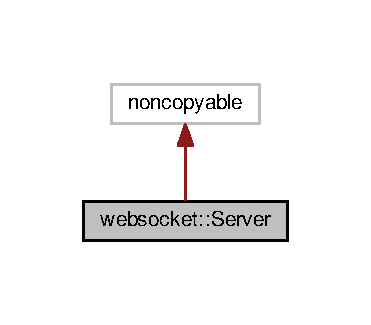
\includegraphics[width=181pt]{classwebsocket_1_1Server__inherit__graph}
\end{center}
\end{figure}


Collaboration diagram for websocket\+:\+:Server\+:
\nopagebreak
\begin{figure}[H]
\begin{center}
\leavevmode
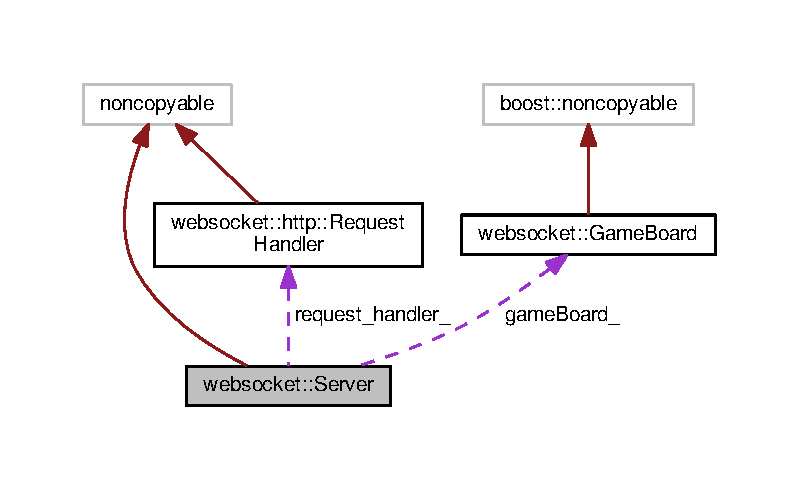
\includegraphics[width=350pt]{classwebsocket_1_1Server__coll__graph}
\end{center}
\end{figure}
\subsection*{Public Member Functions}
\begin{DoxyCompactItemize}
\item 
\hyperlink{classwebsocket_1_1Server_a5a619eb7cc286a2288794f0488441a43}{Server} (const std\+::string \&address, const std\+::string \&port)
\item 
void \hyperlink{classwebsocket_1_1Server_afbc99df156a68d67b6a8ecc82e0b7a57}{run} ()
\begin{DoxyCompactList}\small\item\em Run the \hyperlink{classwebsocket_1_1Server}{Server}\textquotesingle{}s io\+\_\+service loop. \end{DoxyCompactList}\end{DoxyCompactItemize}
\subsection*{Private Member Functions}
\begin{DoxyCompactItemize}
\item 
void \hyperlink{classwebsocket_1_1Server_a01514c0f01fc493222b2d8b877dee540}{start\+\_\+accept} ()
\begin{DoxyCompactList}\small\item\em Initiate an asynchronous accept operation. \end{DoxyCompactList}\item 
void \hyperlink{classwebsocket_1_1Server_a3c14a674a090698e82fc59db5df4b3c4}{handle\+\_\+accept} (const boost\+::system\+::error\+\_\+code \&e)
\begin{DoxyCompactList}\small\item\em Handle completion of an asynchronous accept operation. \end{DoxyCompactList}\item 
void \hyperlink{classwebsocket_1_1Server_a4abf8e0742d15023f0ac95ced8aee07a}{handle\+\_\+stop} ()
\begin{DoxyCompactList}\small\item\em Handle a Request to stop the \hyperlink{classwebsocket_1_1Server}{Server}. \end{DoxyCompactList}\end{DoxyCompactItemize}
\subsection*{Private Attributes}
\begin{DoxyCompactItemize}
\item 
boost\+::asio\+::io\+\_\+service \hyperlink{classwebsocket_1_1Server_ab3dc5f36bb4b0913c803915d3191a771}{io\+\_\+service\+\_\+}
\begin{DoxyCompactList}\small\item\em The io\+\_\+service used to perform asynchronous operations. \end{DoxyCompactList}\item 
boost\+::asio\+::signal\+\_\+set \hyperlink{classwebsocket_1_1Server_a85a9160e9b9f070a4bf8e149623a5a6d}{signals\+\_\+}
\begin{DoxyCompactList}\small\item\em The signal\+\_\+set is used to register for process termination notifications. \end{DoxyCompactList}\item 
boost\+::asio\+::ip\+::tcp\+::acceptor \hyperlink{classwebsocket_1_1Server_a377152422807e2f13cc1c6bb18fb416f}{acceptor\+\_\+}
\begin{DoxyCompactList}\small\item\em Acceptor used to listen for incoming connections. \end{DoxyCompactList}\item 
\hyperlink{namespacewebsocket_a12d8500a66e77dc9bfbff046b86714d8}{session\+\_\+ptr} \hyperlink{classwebsocket_1_1Server_a86916b413a3577cb17aed4cda031691e}{new\+\_\+session\+\_\+}
\begin{DoxyCompactList}\small\item\em The next connection to be accepted. \end{DoxyCompactList}\item 
\hyperlink{classwebsocket_1_1http_1_1RequestHandler}{http\+::\+Request\+Handler} \hyperlink{classwebsocket_1_1Server_abee763cfdb56554f90a98ed4b2fc2600}{request\+\_\+handler\+\_\+}
\begin{DoxyCompactList}\small\item\em The handler for all incoming requests. \end{DoxyCompactList}\item 
\hyperlink{classwebsocket_1_1GameBoard}{Game\+Board} \hyperlink{classwebsocket_1_1Server_a412c87233cbe63db77ba955f413c5ef0}{game\+Board\+\_\+}
\begin{DoxyCompactList}\small\item\em The chat game\+\_\+board. \end{DoxyCompactList}\end{DoxyCompactItemize}


\subsection{Constructor \& Destructor Documentation}
\index{websocket\+::\+Server@{websocket\+::\+Server}!Server@{Server}}
\index{Server@{Server}!websocket\+::\+Server@{websocket\+::\+Server}}
\subsubsection[{\texorpdfstring{Server(const std\+::string \&address, const std\+::string \&port)}{Server(const std::string &address, const std::string &port)}}]{\setlength{\rightskip}{0pt plus 5cm}websocket\+::\+Server\+::\+Server (
\begin{DoxyParamCaption}
\item[{const std\+::string \&}]{address, }
\item[{const std\+::string \&}]{port}
\end{DoxyParamCaption}
)\hspace{0.3cm}{\ttfamily [explicit]}}\hypertarget{classwebsocket_1_1Server_a5a619eb7cc286a2288794f0488441a43}{}\label{classwebsocket_1_1Server_a5a619eb7cc286a2288794f0488441a43}
Construct the \hyperlink{classwebsocket_1_1Server}{Server} to listen on the specified T\+CP address and port, and serve up files from the given directory. 

\subsection{Member Function Documentation}
\index{websocket\+::\+Server@{websocket\+::\+Server}!handle\+\_\+accept@{handle\+\_\+accept}}
\index{handle\+\_\+accept@{handle\+\_\+accept}!websocket\+::\+Server@{websocket\+::\+Server}}
\subsubsection[{\texorpdfstring{handle\+\_\+accept(const boost\+::system\+::error\+\_\+code \&e)}{handle_accept(const boost::system::error_code &e)}}]{\setlength{\rightskip}{0pt plus 5cm}void websocket\+::\+Server\+::handle\+\_\+accept (
\begin{DoxyParamCaption}
\item[{const boost\+::system\+::error\+\_\+code \&}]{e}
\end{DoxyParamCaption}
)\hspace{0.3cm}{\ttfamily [private]}}\hypertarget{classwebsocket_1_1Server_a3c14a674a090698e82fc59db5df4b3c4}{}\label{classwebsocket_1_1Server_a3c14a674a090698e82fc59db5df4b3c4}


Handle completion of an asynchronous accept operation. 

\index{websocket\+::\+Server@{websocket\+::\+Server}!handle\+\_\+stop@{handle\+\_\+stop}}
\index{handle\+\_\+stop@{handle\+\_\+stop}!websocket\+::\+Server@{websocket\+::\+Server}}
\subsubsection[{\texorpdfstring{handle\+\_\+stop()}{handle_stop()}}]{\setlength{\rightskip}{0pt plus 5cm}void websocket\+::\+Server\+::handle\+\_\+stop (
\begin{DoxyParamCaption}
{}
\end{DoxyParamCaption}
)\hspace{0.3cm}{\ttfamily [private]}}\hypertarget{classwebsocket_1_1Server_a4abf8e0742d15023f0ac95ced8aee07a}{}\label{classwebsocket_1_1Server_a4abf8e0742d15023f0ac95ced8aee07a}


Handle a Request to stop the \hyperlink{classwebsocket_1_1Server}{Server}. 

\index{websocket\+::\+Server@{websocket\+::\+Server}!run@{run}}
\index{run@{run}!websocket\+::\+Server@{websocket\+::\+Server}}
\subsubsection[{\texorpdfstring{run()}{run()}}]{\setlength{\rightskip}{0pt plus 5cm}void websocket\+::\+Server\+::run (
\begin{DoxyParamCaption}
{}
\end{DoxyParamCaption}
)}\hypertarget{classwebsocket_1_1Server_afbc99df156a68d67b6a8ecc82e0b7a57}{}\label{classwebsocket_1_1Server_afbc99df156a68d67b6a8ecc82e0b7a57}


Run the \hyperlink{classwebsocket_1_1Server}{Server}\textquotesingle{}s io\+\_\+service loop. 

\index{websocket\+::\+Server@{websocket\+::\+Server}!start\+\_\+accept@{start\+\_\+accept}}
\index{start\+\_\+accept@{start\+\_\+accept}!websocket\+::\+Server@{websocket\+::\+Server}}
\subsubsection[{\texorpdfstring{start\+\_\+accept()}{start_accept()}}]{\setlength{\rightskip}{0pt plus 5cm}void websocket\+::\+Server\+::start\+\_\+accept (
\begin{DoxyParamCaption}
{}
\end{DoxyParamCaption}
)\hspace{0.3cm}{\ttfamily [private]}}\hypertarget{classwebsocket_1_1Server_a01514c0f01fc493222b2d8b877dee540}{}\label{classwebsocket_1_1Server_a01514c0f01fc493222b2d8b877dee540}


Initiate an asynchronous accept operation. 



\subsection{Member Data Documentation}
\index{websocket\+::\+Server@{websocket\+::\+Server}!acceptor\+\_\+@{acceptor\+\_\+}}
\index{acceptor\+\_\+@{acceptor\+\_\+}!websocket\+::\+Server@{websocket\+::\+Server}}
\subsubsection[{\texorpdfstring{acceptor\+\_\+}{acceptor_}}]{\setlength{\rightskip}{0pt plus 5cm}boost\+::asio\+::ip\+::tcp\+::acceptor websocket\+::\+Server\+::acceptor\+\_\+\hspace{0.3cm}{\ttfamily [private]}}\hypertarget{classwebsocket_1_1Server_a377152422807e2f13cc1c6bb18fb416f}{}\label{classwebsocket_1_1Server_a377152422807e2f13cc1c6bb18fb416f}


Acceptor used to listen for incoming connections. 

\index{websocket\+::\+Server@{websocket\+::\+Server}!game\+Board\+\_\+@{game\+Board\+\_\+}}
\index{game\+Board\+\_\+@{game\+Board\+\_\+}!websocket\+::\+Server@{websocket\+::\+Server}}
\subsubsection[{\texorpdfstring{game\+Board\+\_\+}{gameBoard_}}]{\setlength{\rightskip}{0pt plus 5cm}{\bf Game\+Board} websocket\+::\+Server\+::game\+Board\+\_\+\hspace{0.3cm}{\ttfamily [private]}}\hypertarget{classwebsocket_1_1Server_a412c87233cbe63db77ba955f413c5ef0}{}\label{classwebsocket_1_1Server_a412c87233cbe63db77ba955f413c5ef0}


The chat game\+\_\+board. 

\index{websocket\+::\+Server@{websocket\+::\+Server}!io\+\_\+service\+\_\+@{io\+\_\+service\+\_\+}}
\index{io\+\_\+service\+\_\+@{io\+\_\+service\+\_\+}!websocket\+::\+Server@{websocket\+::\+Server}}
\subsubsection[{\texorpdfstring{io\+\_\+service\+\_\+}{io_service_}}]{\setlength{\rightskip}{0pt plus 5cm}boost\+::asio\+::io\+\_\+service websocket\+::\+Server\+::io\+\_\+service\+\_\+\hspace{0.3cm}{\ttfamily [private]}}\hypertarget{classwebsocket_1_1Server_ab3dc5f36bb4b0913c803915d3191a771}{}\label{classwebsocket_1_1Server_ab3dc5f36bb4b0913c803915d3191a771}


The io\+\_\+service used to perform asynchronous operations. 

\index{websocket\+::\+Server@{websocket\+::\+Server}!new\+\_\+session\+\_\+@{new\+\_\+session\+\_\+}}
\index{new\+\_\+session\+\_\+@{new\+\_\+session\+\_\+}!websocket\+::\+Server@{websocket\+::\+Server}}
\subsubsection[{\texorpdfstring{new\+\_\+session\+\_\+}{new_session_}}]{\setlength{\rightskip}{0pt plus 5cm}{\bf session\+\_\+ptr} websocket\+::\+Server\+::new\+\_\+session\+\_\+\hspace{0.3cm}{\ttfamily [private]}}\hypertarget{classwebsocket_1_1Server_a86916b413a3577cb17aed4cda031691e}{}\label{classwebsocket_1_1Server_a86916b413a3577cb17aed4cda031691e}


The next connection to be accepted. 

\index{websocket\+::\+Server@{websocket\+::\+Server}!request\+\_\+handler\+\_\+@{request\+\_\+handler\+\_\+}}
\index{request\+\_\+handler\+\_\+@{request\+\_\+handler\+\_\+}!websocket\+::\+Server@{websocket\+::\+Server}}
\subsubsection[{\texorpdfstring{request\+\_\+handler\+\_\+}{request_handler_}}]{\setlength{\rightskip}{0pt plus 5cm}{\bf http\+::\+Request\+Handler} websocket\+::\+Server\+::request\+\_\+handler\+\_\+\hspace{0.3cm}{\ttfamily [private]}}\hypertarget{classwebsocket_1_1Server_abee763cfdb56554f90a98ed4b2fc2600}{}\label{classwebsocket_1_1Server_abee763cfdb56554f90a98ed4b2fc2600}


The handler for all incoming requests. 

\index{websocket\+::\+Server@{websocket\+::\+Server}!signals\+\_\+@{signals\+\_\+}}
\index{signals\+\_\+@{signals\+\_\+}!websocket\+::\+Server@{websocket\+::\+Server}}
\subsubsection[{\texorpdfstring{signals\+\_\+}{signals_}}]{\setlength{\rightskip}{0pt plus 5cm}boost\+::asio\+::signal\+\_\+set websocket\+::\+Server\+::signals\+\_\+\hspace{0.3cm}{\ttfamily [private]}}\hypertarget{classwebsocket_1_1Server_a85a9160e9b9f070a4bf8e149623a5a6d}{}\label{classwebsocket_1_1Server_a85a9160e9b9f070a4bf8e149623a5a6d}


The signal\+\_\+set is used to register for process termination notifications. 



The documentation for this class was generated from the following files\+:\begin{DoxyCompactItemize}
\item 
\hyperlink{server_8hpp}{server.\+hpp}\item 
\hyperlink{server_8cpp}{server.\+cpp}\end{DoxyCompactItemize}

\hypertarget{classwebsocket_1_1Session}{}\section{websocket\+:\+:Session Class Reference}
\label{classwebsocket_1_1Session}\index{websocket\+::\+Session@{websocket\+::\+Session}}


{\ttfamily \#include $<$session.\+hpp$>$}



Inheritance diagram for websocket\+:\+:Session\+:\nopagebreak
\begin{figure}[H]
\begin{center}
\leavevmode
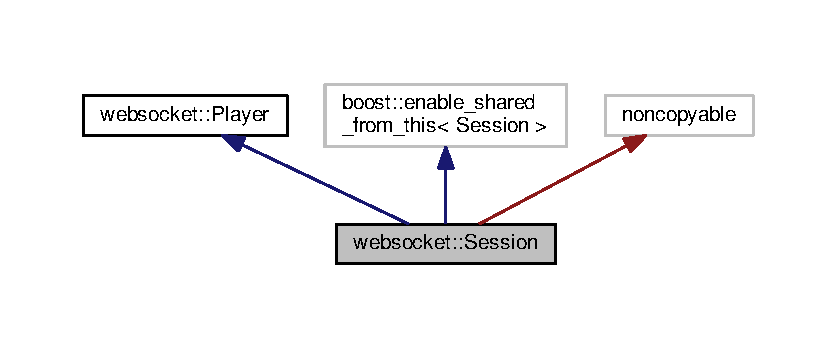
\includegraphics[width=350pt]{classwebsocket_1_1Session__inherit__graph}
\end{center}
\end{figure}


Collaboration diagram for websocket\+:\+:Session\+:
\nopagebreak
\begin{figure}[H]
\begin{center}
\leavevmode
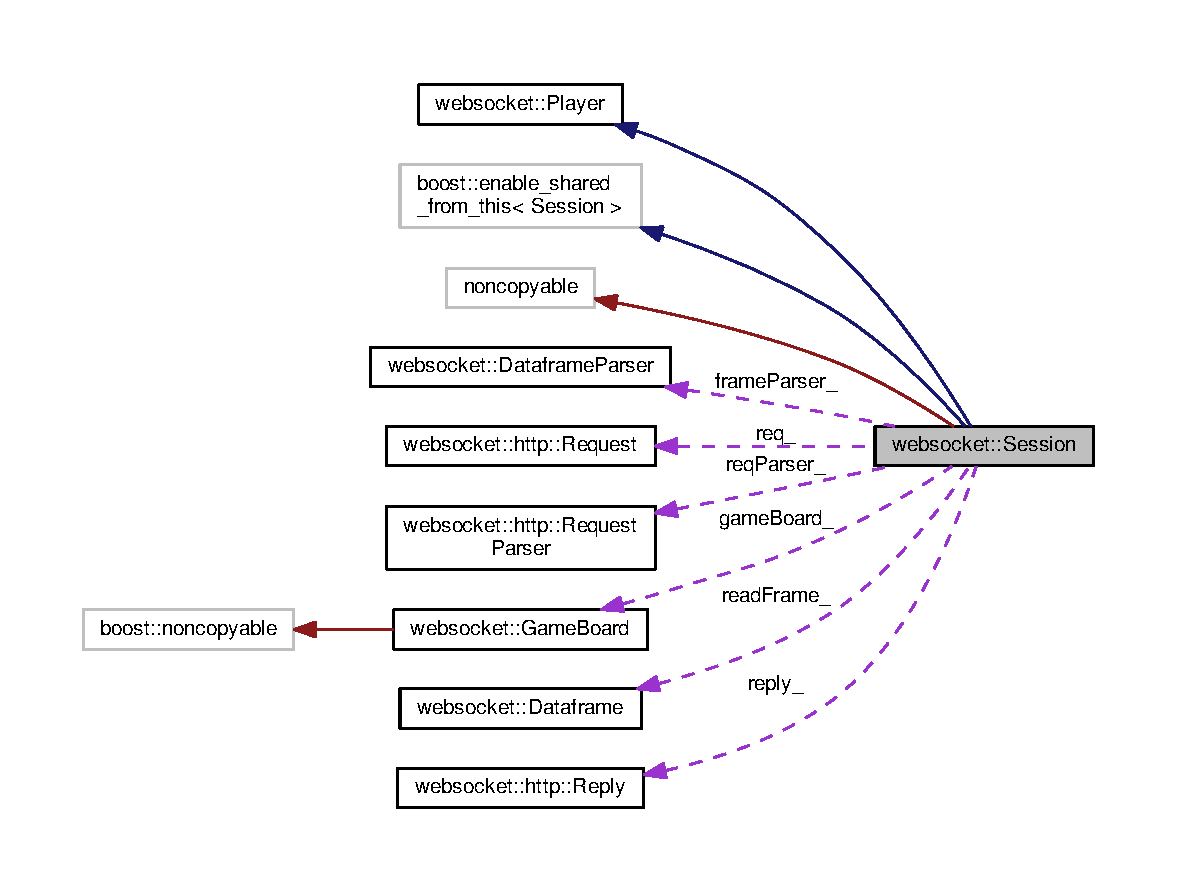
\includegraphics[width=350pt]{classwebsocket_1_1Session__coll__graph}
\end{center}
\end{figure}
\subsection*{Public Types}
\begin{DoxyCompactItemize}
\item 
enum \hyperlink{classwebsocket_1_1Session_a643e11bb9d05b580f20ff232f3582c1b}{state} \{ \\*
\hyperlink{classwebsocket_1_1Session_a643e11bb9d05b580f20ff232f3582c1baea725805737e434c2b1d0b061df4ddde}{U\+N\+D\+E\+F\+I\+N\+E\+D\+\_\+\+S\+T\+A\+TE}, 
\hyperlink{classwebsocket_1_1Session_a643e11bb9d05b580f20ff232f3582c1ba3b14b5a3d2ab8b61422448f7464a5d4a}{R\+E\+A\+D\+I\+N\+G\+\_\+\+H\+A\+N\+D\+S\+H\+A\+KE}, 
\hyperlink{classwebsocket_1_1Session_a643e11bb9d05b580f20ff232f3582c1ba057f3e49a1f4623a6011d712c1cbc7ba}{B\+A\+D\+\_\+\+R\+E\+Q\+U\+E\+ST}, 
\hyperlink{classwebsocket_1_1Session_a643e11bb9d05b580f20ff232f3582c1ba272f56d02b3f719d25d23ebe3f68f44a}{W\+R\+I\+T\+I\+N\+G\+\_\+\+H\+A\+N\+D\+S\+H\+A\+KE}, 
\\*
\hyperlink{classwebsocket_1_1Session_a643e11bb9d05b580f20ff232f3582c1baba12c4de6ae83a4f63b1c700d4ecfe8e}{P\+U\+M\+P\+I\+N\+G\+\_\+\+M\+E\+S\+S\+A\+G\+ES}
 \}\begin{DoxyCompactList}\small\item\em The \hyperlink{classwebsocket_1_1Session}{Session} states. \end{DoxyCompactList}
\end{DoxyCompactItemize}
\subsection*{Public Member Functions}
\begin{DoxyCompactItemize}
\item 
\hyperlink{classwebsocket_1_1Session_ac24bab7092bff9d7a6deaa6b94e73a87}{Session} (boost\+::asio\+::io\+\_\+service \&io\+\_\+service, \hyperlink{classwebsocket_1_1GameBoard}{Game\+Board} \&game\+\_\+board)
\begin{DoxyCompactList}\small\item\em Construct a connection with the given io\+\_\+service. \end{DoxyCompactList}\item 
boost\+::asio\+::ip\+::tcp\+::socket \& \hyperlink{classwebsocket_1_1Session_a0c5a4e7b9ca4c0e01a55c4c528470a76}{socket} ()
\begin{DoxyCompactList}\small\item\em Get the socket associated with the connection. \end{DoxyCompactList}\item 
void \hyperlink{classwebsocket_1_1Session_a0d9852b26f06d0860e9535b2e36b7d88}{start} ()
\begin{DoxyCompactList}\small\item\em Start the first asynchronous operation for the connection. \end{DoxyCompactList}\end{DoxyCompactItemize}
\subsection*{Public Attributes}
\begin{DoxyCompactItemize}
\item 
enum \hyperlink{classwebsocket_1_1Session_a643e11bb9d05b580f20ff232f3582c1b}{websocket\+::\+Session\+::state} \hyperlink{classwebsocket_1_1Session_a8f9e0d65f4de675dd7b8242e17ee29b7}{state\+\_\+}
\end{DoxyCompactItemize}
\subsection*{Private Member Functions}
\begin{DoxyCompactItemize}
\item 
void \hyperlink{classwebsocket_1_1Session_ad23257dd2bffa48e90ed9941d39ca56b}{handle\+\_\+read} (const boost\+::system\+::error\+\_\+code \&e, std\+::size\+\_\+t bytes\+\_\+transferred)
\begin{DoxyCompactList}\small\item\em Handle completion of a read operation. \end{DoxyCompactList}\item 
void \hyperlink{classwebsocket_1_1Session_aa3912eefe7b2d125d0f3739c96f98a83}{handle\+\_\+write} (const boost\+::system\+::error\+\_\+code \&e)
\begin{DoxyCompactList}\small\item\em Handle completion of a write operation. \end{DoxyCompactList}\item 
void \hyperlink{classwebsocket_1_1Session_a6af4fbb5ea959b9e079e779a887c4f27}{deliver} (\hyperlink{structwebsocket_1_1Dataframe}{Dataframe} msg)
\begin{DoxyCompactList}\small\item\em Deliver a message to the client. \end{DoxyCompactList}\item 
std\+::string \hyperlink{classwebsocket_1_1Session_a1da5647ac33cae9b350b586a25297323}{get\+Id} ()
\begin{DoxyCompactList}\small\item\em Get the client id. \end{DoxyCompactList}\end{DoxyCompactItemize}
\subsection*{Private Attributes}
\begin{DoxyCompactItemize}
\item 
boost\+::asio\+::io\+\_\+service\+::strand \hyperlink{classwebsocket_1_1Session_a394bb9b578c166e22b2a630b8ea013fb}{strand\+\_\+}
\begin{DoxyCompactList}\small\item\em Strand to ensure the connection\textquotesingle{}s handlers are not called concurrently. \end{DoxyCompactList}\item 
boost\+::asio\+::ip\+::tcp\+::socket \hyperlink{classwebsocket_1_1Session_a7e7771fef3f105f4019ef9a1c2f04eb5}{socket\+\_\+}
\begin{DoxyCompactList}\small\item\em Socket for the connection. \end{DoxyCompactList}\item 
\hyperlink{classwebsocket_1_1GameBoard}{Game\+Board} \& \hyperlink{classwebsocket_1_1Session_add75c0a25f69839df5441997846b3f3e}{game\+Board\+\_\+}
\begin{DoxyCompactList}\small\item\em The chat game\+\_\+board where the messages will be posted. \end{DoxyCompactList}\item 
boost\+::array$<$ boost\+::uint8\+\_\+t, 8192 $>$ \hyperlink{classwebsocket_1_1Session_a4a7ca92db9c843899fbf3673fe5b9f52}{buff\+\_\+}
\begin{DoxyCompactList}\small\item\em The buffer for incoming data. \end{DoxyCompactList}\item 
\hyperlink{structwebsocket_1_1http_1_1Request}{http\+::\+Request} \hyperlink{classwebsocket_1_1Session_a80b1e6b3657a3c3528acd3c9b4e453a5}{req\+\_\+}
\begin{DoxyCompactList}\small\item\em The incoming http request. \end{DoxyCompactList}\item 
\hyperlink{classwebsocket_1_1http_1_1RequestParser}{http\+::\+Request\+Parser} \hyperlink{classwebsocket_1_1Session_a0336ca414e7c038331b39a01cdb23da8}{req\+Parser\+\_\+}
\begin{DoxyCompactList}\small\item\em The parser for the incoming http request. \end{DoxyCompactList}\item 
\hyperlink{structwebsocket_1_1http_1_1Reply}{http\+::\+Reply} \hyperlink{classwebsocket_1_1Session_a938563bfc401a7446f87a60acc642800}{reply\+\_\+}
\begin{DoxyCompactList}\small\item\em The http Reply to be sent back to the client. \end{DoxyCompactList}\item 
\hyperlink{classwebsocket_1_1DataframeParser}{Dataframe\+Parser} \hyperlink{classwebsocket_1_1Session_add7f041fe3badd9bea5158a412d4c33b}{frame\+Parser\+\_\+}
\begin{DoxyCompactList}\small\item\em The parser for the incoming messages. \end{DoxyCompactList}\item 
\hyperlink{structwebsocket_1_1Dataframe}{Dataframe} \hyperlink{classwebsocket_1_1Session_a2ea49f75569589cc80cb9dbcfa7707ee}{read\+Frame\+\_\+}
\begin{DoxyCompactList}\small\item\em The incoming message. \end{DoxyCompactList}\item 
\hyperlink{namespacewebsocket_ae3fdf29bb367b5baf5be703253a4edfa}{message\+\_\+queue} \hyperlink{classwebsocket_1_1Session_ace231022157030f4d56de9bfeff43ac7}{write\+Msgs\+\_\+}
\begin{DoxyCompactList}\small\item\em The messages to be sent to the client. \end{DoxyCompactList}\end{DoxyCompactItemize}


\subsection{Member Enumeration Documentation}
\index{websocket\+::\+Session@{websocket\+::\+Session}!state@{state}}
\index{state@{state}!websocket\+::\+Session@{websocket\+::\+Session}}
\subsubsection[{\texorpdfstring{state}{state}}]{\setlength{\rightskip}{0pt plus 5cm}enum {\bf websocket\+::\+Session\+::state}}\hypertarget{classwebsocket_1_1Session_a643e11bb9d05b580f20ff232f3582c1b}{}\label{classwebsocket_1_1Session_a643e11bb9d05b580f20ff232f3582c1b}


The \hyperlink{classwebsocket_1_1Session}{Session} states. 

\begin{Desc}
\item[Enumerator]\par
\begin{description}
\index{U\+N\+D\+E\+F\+I\+N\+E\+D\+\_\+\+S\+T\+A\+TE@{U\+N\+D\+E\+F\+I\+N\+E\+D\+\_\+\+S\+T\+A\+TE}!websocket\+::\+Session@{websocket\+::\+Session}}\index{websocket\+::\+Session@{websocket\+::\+Session}!U\+N\+D\+E\+F\+I\+N\+E\+D\+\_\+\+S\+T\+A\+TE@{U\+N\+D\+E\+F\+I\+N\+E\+D\+\_\+\+S\+T\+A\+TE}}\item[{\em 
U\+N\+D\+E\+F\+I\+N\+E\+D\+\_\+\+S\+T\+A\+TE\hypertarget{classwebsocket_1_1Session_a643e11bb9d05b580f20ff232f3582c1baea725805737e434c2b1d0b061df4ddde}{}\label{classwebsocket_1_1Session_a643e11bb9d05b580f20ff232f3582c1baea725805737e434c2b1d0b061df4ddde}
}]\index{R\+E\+A\+D\+I\+N\+G\+\_\+\+H\+A\+N\+D\+S\+H\+A\+KE@{R\+E\+A\+D\+I\+N\+G\+\_\+\+H\+A\+N\+D\+S\+H\+A\+KE}!websocket\+::\+Session@{websocket\+::\+Session}}\index{websocket\+::\+Session@{websocket\+::\+Session}!R\+E\+A\+D\+I\+N\+G\+\_\+\+H\+A\+N\+D\+S\+H\+A\+KE@{R\+E\+A\+D\+I\+N\+G\+\_\+\+H\+A\+N\+D\+S\+H\+A\+KE}}\item[{\em 
R\+E\+A\+D\+I\+N\+G\+\_\+\+H\+A\+N\+D\+S\+H\+A\+KE\hypertarget{classwebsocket_1_1Session_a643e11bb9d05b580f20ff232f3582c1ba3b14b5a3d2ab8b61422448f7464a5d4a}{}\label{classwebsocket_1_1Session_a643e11bb9d05b580f20ff232f3582c1ba3b14b5a3d2ab8b61422448f7464a5d4a}
}]\index{B\+A\+D\+\_\+\+R\+E\+Q\+U\+E\+ST@{B\+A\+D\+\_\+\+R\+E\+Q\+U\+E\+ST}!websocket\+::\+Session@{websocket\+::\+Session}}\index{websocket\+::\+Session@{websocket\+::\+Session}!B\+A\+D\+\_\+\+R\+E\+Q\+U\+E\+ST@{B\+A\+D\+\_\+\+R\+E\+Q\+U\+E\+ST}}\item[{\em 
B\+A\+D\+\_\+\+R\+E\+Q\+U\+E\+ST\hypertarget{classwebsocket_1_1Session_a643e11bb9d05b580f20ff232f3582c1ba057f3e49a1f4623a6011d712c1cbc7ba}{}\label{classwebsocket_1_1Session_a643e11bb9d05b580f20ff232f3582c1ba057f3e49a1f4623a6011d712c1cbc7ba}
}]\index{W\+R\+I\+T\+I\+N\+G\+\_\+\+H\+A\+N\+D\+S\+H\+A\+KE@{W\+R\+I\+T\+I\+N\+G\+\_\+\+H\+A\+N\+D\+S\+H\+A\+KE}!websocket\+::\+Session@{websocket\+::\+Session}}\index{websocket\+::\+Session@{websocket\+::\+Session}!W\+R\+I\+T\+I\+N\+G\+\_\+\+H\+A\+N\+D\+S\+H\+A\+KE@{W\+R\+I\+T\+I\+N\+G\+\_\+\+H\+A\+N\+D\+S\+H\+A\+KE}}\item[{\em 
W\+R\+I\+T\+I\+N\+G\+\_\+\+H\+A\+N\+D\+S\+H\+A\+KE\hypertarget{classwebsocket_1_1Session_a643e11bb9d05b580f20ff232f3582c1ba272f56d02b3f719d25d23ebe3f68f44a}{}\label{classwebsocket_1_1Session_a643e11bb9d05b580f20ff232f3582c1ba272f56d02b3f719d25d23ebe3f68f44a}
}]\index{P\+U\+M\+P\+I\+N\+G\+\_\+\+M\+E\+S\+S\+A\+G\+ES@{P\+U\+M\+P\+I\+N\+G\+\_\+\+M\+E\+S\+S\+A\+G\+ES}!websocket\+::\+Session@{websocket\+::\+Session}}\index{websocket\+::\+Session@{websocket\+::\+Session}!P\+U\+M\+P\+I\+N\+G\+\_\+\+M\+E\+S\+S\+A\+G\+ES@{P\+U\+M\+P\+I\+N\+G\+\_\+\+M\+E\+S\+S\+A\+G\+ES}}\item[{\em 
P\+U\+M\+P\+I\+N\+G\+\_\+\+M\+E\+S\+S\+A\+G\+ES\hypertarget{classwebsocket_1_1Session_a643e11bb9d05b580f20ff232f3582c1baba12c4de6ae83a4f63b1c700d4ecfe8e}{}\label{classwebsocket_1_1Session_a643e11bb9d05b580f20ff232f3582c1baba12c4de6ae83a4f63b1c700d4ecfe8e}
}]\end{description}
\end{Desc}


\subsection{Constructor \& Destructor Documentation}
\index{websocket\+::\+Session@{websocket\+::\+Session}!Session@{Session}}
\index{Session@{Session}!websocket\+::\+Session@{websocket\+::\+Session}}
\subsubsection[{\texorpdfstring{Session(boost\+::asio\+::io\+\_\+service \&io\+\_\+service, Game\+Board \&game\+\_\+board)}{Session(boost::asio::io_service &io_service, GameBoard &game_board)}}]{\setlength{\rightskip}{0pt plus 5cm}websocket\+::\+Session\+::\+Session (
\begin{DoxyParamCaption}
\item[{boost\+::asio\+::io\+\_\+service \&}]{io\+\_\+service, }
\item[{{\bf Game\+Board} \&}]{game\+\_\+board}
\end{DoxyParamCaption}
)\hspace{0.3cm}{\ttfamily [explicit]}}\hypertarget{classwebsocket_1_1Session_ac24bab7092bff9d7a6deaa6b94e73a87}{}\label{classwebsocket_1_1Session_ac24bab7092bff9d7a6deaa6b94e73a87}


Construct a connection with the given io\+\_\+service. 



\subsection{Member Function Documentation}
\index{websocket\+::\+Session@{websocket\+::\+Session}!deliver@{deliver}}
\index{deliver@{deliver}!websocket\+::\+Session@{websocket\+::\+Session}}
\subsubsection[{\texorpdfstring{deliver(\+Dataframe msg)}{deliver(Dataframe msg)}}]{\setlength{\rightskip}{0pt plus 5cm}void websocket\+::\+Session\+::deliver (
\begin{DoxyParamCaption}
\item[{{\bf Dataframe}}]{msg}
\end{DoxyParamCaption}
)\hspace{0.3cm}{\ttfamily [private]}, {\ttfamily [virtual]}}\hypertarget{classwebsocket_1_1Session_a6af4fbb5ea959b9e079e779a887c4f27}{}\label{classwebsocket_1_1Session_a6af4fbb5ea959b9e079e779a887c4f27}


Deliver a message to the client. 



Implements \hyperlink{classwebsocket_1_1Player_adf19a07c6497129268b3719783e7180d}{websocket\+::\+Player}.

\index{websocket\+::\+Session@{websocket\+::\+Session}!get\+Id@{get\+Id}}
\index{get\+Id@{get\+Id}!websocket\+::\+Session@{websocket\+::\+Session}}
\subsubsection[{\texorpdfstring{get\+Id()}{getId()}}]{\setlength{\rightskip}{0pt plus 5cm}std\+::string websocket\+::\+Session\+::get\+Id (
\begin{DoxyParamCaption}
{}
\end{DoxyParamCaption}
)\hspace{0.3cm}{\ttfamily [private]}, {\ttfamily [virtual]}}\hypertarget{classwebsocket_1_1Session_a1da5647ac33cae9b350b586a25297323}{}\label{classwebsocket_1_1Session_a1da5647ac33cae9b350b586a25297323}


Get the client id. 



Implements \hyperlink{classwebsocket_1_1Player_a440338aee24d324c46115bc7b4c7a463}{websocket\+::\+Player}.

\index{websocket\+::\+Session@{websocket\+::\+Session}!handle\+\_\+read@{handle\+\_\+read}}
\index{handle\+\_\+read@{handle\+\_\+read}!websocket\+::\+Session@{websocket\+::\+Session}}
\subsubsection[{\texorpdfstring{handle\+\_\+read(const boost\+::system\+::error\+\_\+code \&e, std\+::size\+\_\+t bytes\+\_\+transferred)}{handle_read(const boost::system::error_code &e, std::size_t bytes_transferred)}}]{\setlength{\rightskip}{0pt plus 5cm}void websocket\+::\+Session\+::handle\+\_\+read (
\begin{DoxyParamCaption}
\item[{const boost\+::system\+::error\+\_\+code \&}]{e, }
\item[{std\+::size\+\_\+t}]{bytes\+\_\+transferred}
\end{DoxyParamCaption}
)\hspace{0.3cm}{\ttfamily [private]}}\hypertarget{classwebsocket_1_1Session_ad23257dd2bffa48e90ed9941d39ca56b}{}\label{classwebsocket_1_1Session_ad23257dd2bffa48e90ed9941d39ca56b}


Handle completion of a read operation. 

\index{websocket\+::\+Session@{websocket\+::\+Session}!handle\+\_\+write@{handle\+\_\+write}}
\index{handle\+\_\+write@{handle\+\_\+write}!websocket\+::\+Session@{websocket\+::\+Session}}
\subsubsection[{\texorpdfstring{handle\+\_\+write(const boost\+::system\+::error\+\_\+code \&e)}{handle_write(const boost::system::error_code &e)}}]{\setlength{\rightskip}{0pt plus 5cm}void websocket\+::\+Session\+::handle\+\_\+write (
\begin{DoxyParamCaption}
\item[{const boost\+::system\+::error\+\_\+code \&}]{e}
\end{DoxyParamCaption}
)\hspace{0.3cm}{\ttfamily [private]}}\hypertarget{classwebsocket_1_1Session_aa3912eefe7b2d125d0f3739c96f98a83}{}\label{classwebsocket_1_1Session_aa3912eefe7b2d125d0f3739c96f98a83}


Handle completion of a write operation. 

\index{websocket\+::\+Session@{websocket\+::\+Session}!socket@{socket}}
\index{socket@{socket}!websocket\+::\+Session@{websocket\+::\+Session}}
\subsubsection[{\texorpdfstring{socket()}{socket()}}]{\setlength{\rightskip}{0pt plus 5cm}boost\+::asio\+::ip\+::tcp\+::socket \& websocket\+::\+Session\+::socket (
\begin{DoxyParamCaption}
{}
\end{DoxyParamCaption}
)}\hypertarget{classwebsocket_1_1Session_a0c5a4e7b9ca4c0e01a55c4c528470a76}{}\label{classwebsocket_1_1Session_a0c5a4e7b9ca4c0e01a55c4c528470a76}


Get the socket associated with the connection. 

\index{websocket\+::\+Session@{websocket\+::\+Session}!start@{start}}
\index{start@{start}!websocket\+::\+Session@{websocket\+::\+Session}}
\subsubsection[{\texorpdfstring{start()}{start()}}]{\setlength{\rightskip}{0pt plus 5cm}void websocket\+::\+Session\+::start (
\begin{DoxyParamCaption}
{}
\end{DoxyParamCaption}
)}\hypertarget{classwebsocket_1_1Session_a0d9852b26f06d0860e9535b2e36b7d88}{}\label{classwebsocket_1_1Session_a0d9852b26f06d0860e9535b2e36b7d88}


Start the first asynchronous operation for the connection. 



\subsection{Member Data Documentation}
\index{websocket\+::\+Session@{websocket\+::\+Session}!buff\+\_\+@{buff\+\_\+}}
\index{buff\+\_\+@{buff\+\_\+}!websocket\+::\+Session@{websocket\+::\+Session}}
\subsubsection[{\texorpdfstring{buff\+\_\+}{buff_}}]{\setlength{\rightskip}{0pt plus 5cm}boost\+::array$<$boost\+::uint8\+\_\+t, 8192$>$ websocket\+::\+Session\+::buff\+\_\+\hspace{0.3cm}{\ttfamily [private]}}\hypertarget{classwebsocket_1_1Session_a4a7ca92db9c843899fbf3673fe5b9f52}{}\label{classwebsocket_1_1Session_a4a7ca92db9c843899fbf3673fe5b9f52}


The buffer for incoming data. 

\index{websocket\+::\+Session@{websocket\+::\+Session}!frame\+Parser\+\_\+@{frame\+Parser\+\_\+}}
\index{frame\+Parser\+\_\+@{frame\+Parser\+\_\+}!websocket\+::\+Session@{websocket\+::\+Session}}
\subsubsection[{\texorpdfstring{frame\+Parser\+\_\+}{frameParser_}}]{\setlength{\rightskip}{0pt plus 5cm}{\bf Dataframe\+Parser} websocket\+::\+Session\+::frame\+Parser\+\_\+\hspace{0.3cm}{\ttfamily [private]}}\hypertarget{classwebsocket_1_1Session_add7f041fe3badd9bea5158a412d4c33b}{}\label{classwebsocket_1_1Session_add7f041fe3badd9bea5158a412d4c33b}


The parser for the incoming messages. 

\index{websocket\+::\+Session@{websocket\+::\+Session}!game\+Board\+\_\+@{game\+Board\+\_\+}}
\index{game\+Board\+\_\+@{game\+Board\+\_\+}!websocket\+::\+Session@{websocket\+::\+Session}}
\subsubsection[{\texorpdfstring{game\+Board\+\_\+}{gameBoard_}}]{\setlength{\rightskip}{0pt plus 5cm}{\bf Game\+Board}\& websocket\+::\+Session\+::game\+Board\+\_\+\hspace{0.3cm}{\ttfamily [private]}}\hypertarget{classwebsocket_1_1Session_add75c0a25f69839df5441997846b3f3e}{}\label{classwebsocket_1_1Session_add75c0a25f69839df5441997846b3f3e}


The chat game\+\_\+board where the messages will be posted. 

\index{websocket\+::\+Session@{websocket\+::\+Session}!read\+Frame\+\_\+@{read\+Frame\+\_\+}}
\index{read\+Frame\+\_\+@{read\+Frame\+\_\+}!websocket\+::\+Session@{websocket\+::\+Session}}
\subsubsection[{\texorpdfstring{read\+Frame\+\_\+}{readFrame_}}]{\setlength{\rightskip}{0pt plus 5cm}{\bf Dataframe} websocket\+::\+Session\+::read\+Frame\+\_\+\hspace{0.3cm}{\ttfamily [private]}}\hypertarget{classwebsocket_1_1Session_a2ea49f75569589cc80cb9dbcfa7707ee}{}\label{classwebsocket_1_1Session_a2ea49f75569589cc80cb9dbcfa7707ee}


The incoming message. 

\index{websocket\+::\+Session@{websocket\+::\+Session}!reply\+\_\+@{reply\+\_\+}}
\index{reply\+\_\+@{reply\+\_\+}!websocket\+::\+Session@{websocket\+::\+Session}}
\subsubsection[{\texorpdfstring{reply\+\_\+}{reply_}}]{\setlength{\rightskip}{0pt plus 5cm}{\bf http\+::\+Reply} websocket\+::\+Session\+::reply\+\_\+\hspace{0.3cm}{\ttfamily [private]}}\hypertarget{classwebsocket_1_1Session_a938563bfc401a7446f87a60acc642800}{}\label{classwebsocket_1_1Session_a938563bfc401a7446f87a60acc642800}


The http Reply to be sent back to the client. 

\index{websocket\+::\+Session@{websocket\+::\+Session}!req\+\_\+@{req\+\_\+}}
\index{req\+\_\+@{req\+\_\+}!websocket\+::\+Session@{websocket\+::\+Session}}
\subsubsection[{\texorpdfstring{req\+\_\+}{req_}}]{\setlength{\rightskip}{0pt plus 5cm}{\bf http\+::\+Request} websocket\+::\+Session\+::req\+\_\+\hspace{0.3cm}{\ttfamily [private]}}\hypertarget{classwebsocket_1_1Session_a80b1e6b3657a3c3528acd3c9b4e453a5}{}\label{classwebsocket_1_1Session_a80b1e6b3657a3c3528acd3c9b4e453a5}


The incoming http request. 

\index{websocket\+::\+Session@{websocket\+::\+Session}!req\+Parser\+\_\+@{req\+Parser\+\_\+}}
\index{req\+Parser\+\_\+@{req\+Parser\+\_\+}!websocket\+::\+Session@{websocket\+::\+Session}}
\subsubsection[{\texorpdfstring{req\+Parser\+\_\+}{reqParser_}}]{\setlength{\rightskip}{0pt plus 5cm}{\bf http\+::\+Request\+Parser} websocket\+::\+Session\+::req\+Parser\+\_\+\hspace{0.3cm}{\ttfamily [private]}}\hypertarget{classwebsocket_1_1Session_a0336ca414e7c038331b39a01cdb23da8}{}\label{classwebsocket_1_1Session_a0336ca414e7c038331b39a01cdb23da8}


The parser for the incoming http request. 

\index{websocket\+::\+Session@{websocket\+::\+Session}!socket\+\_\+@{socket\+\_\+}}
\index{socket\+\_\+@{socket\+\_\+}!websocket\+::\+Session@{websocket\+::\+Session}}
\subsubsection[{\texorpdfstring{socket\+\_\+}{socket_}}]{\setlength{\rightskip}{0pt plus 5cm}boost\+::asio\+::ip\+::tcp\+::socket websocket\+::\+Session\+::socket\+\_\+\hspace{0.3cm}{\ttfamily [private]}}\hypertarget{classwebsocket_1_1Session_a7e7771fef3f105f4019ef9a1c2f04eb5}{}\label{classwebsocket_1_1Session_a7e7771fef3f105f4019ef9a1c2f04eb5}


Socket for the connection. 

\index{websocket\+::\+Session@{websocket\+::\+Session}!state\+\_\+@{state\+\_\+}}
\index{state\+\_\+@{state\+\_\+}!websocket\+::\+Session@{websocket\+::\+Session}}
\subsubsection[{\texorpdfstring{state\+\_\+}{state_}}]{\setlength{\rightskip}{0pt plus 5cm}enum {\bf websocket\+::\+Session\+::state}  websocket\+::\+Session\+::state\+\_\+}\hypertarget{classwebsocket_1_1Session_a8f9e0d65f4de675dd7b8242e17ee29b7}{}\label{classwebsocket_1_1Session_a8f9e0d65f4de675dd7b8242e17ee29b7}
\index{websocket\+::\+Session@{websocket\+::\+Session}!strand\+\_\+@{strand\+\_\+}}
\index{strand\+\_\+@{strand\+\_\+}!websocket\+::\+Session@{websocket\+::\+Session}}
\subsubsection[{\texorpdfstring{strand\+\_\+}{strand_}}]{\setlength{\rightskip}{0pt plus 5cm}boost\+::asio\+::io\+\_\+service\+::strand websocket\+::\+Session\+::strand\+\_\+\hspace{0.3cm}{\ttfamily [private]}}\hypertarget{classwebsocket_1_1Session_a394bb9b578c166e22b2a630b8ea013fb}{}\label{classwebsocket_1_1Session_a394bb9b578c166e22b2a630b8ea013fb}


Strand to ensure the connection\textquotesingle{}s handlers are not called concurrently. 

\index{websocket\+::\+Session@{websocket\+::\+Session}!write\+Msgs\+\_\+@{write\+Msgs\+\_\+}}
\index{write\+Msgs\+\_\+@{write\+Msgs\+\_\+}!websocket\+::\+Session@{websocket\+::\+Session}}
\subsubsection[{\texorpdfstring{write\+Msgs\+\_\+}{writeMsgs_}}]{\setlength{\rightskip}{0pt plus 5cm}{\bf message\+\_\+queue} websocket\+::\+Session\+::write\+Msgs\+\_\+\hspace{0.3cm}{\ttfamily [private]}}\hypertarget{classwebsocket_1_1Session_ace231022157030f4d56de9bfeff43ac7}{}\label{classwebsocket_1_1Session_ace231022157030f4d56de9bfeff43ac7}


The messages to be sent to the client. 



The documentation for this class was generated from the following files\+:\begin{DoxyCompactItemize}
\item 
\hyperlink{session_8hpp}{session.\+hpp}\item 
\hyperlink{session_8cpp}{session.\+cpp}\end{DoxyCompactItemize}

\chapter{File Documentation}
\hypertarget{ball_8cpp}{}\section{ball.\+cpp File Reference}
\label{ball_8cpp}\index{ball.\+cpp@{ball.\+cpp}}
{\ttfamily \#include \char`\"{}ball.\+hpp\char`\"{}}\\*
{\ttfamily \#include \char`\"{}game\+\_\+board.\+hpp\char`\"{}}\\*
Include dependency graph for ball.\+cpp\+:
\nopagebreak
\begin{figure}[H]
\begin{center}
\leavevmode
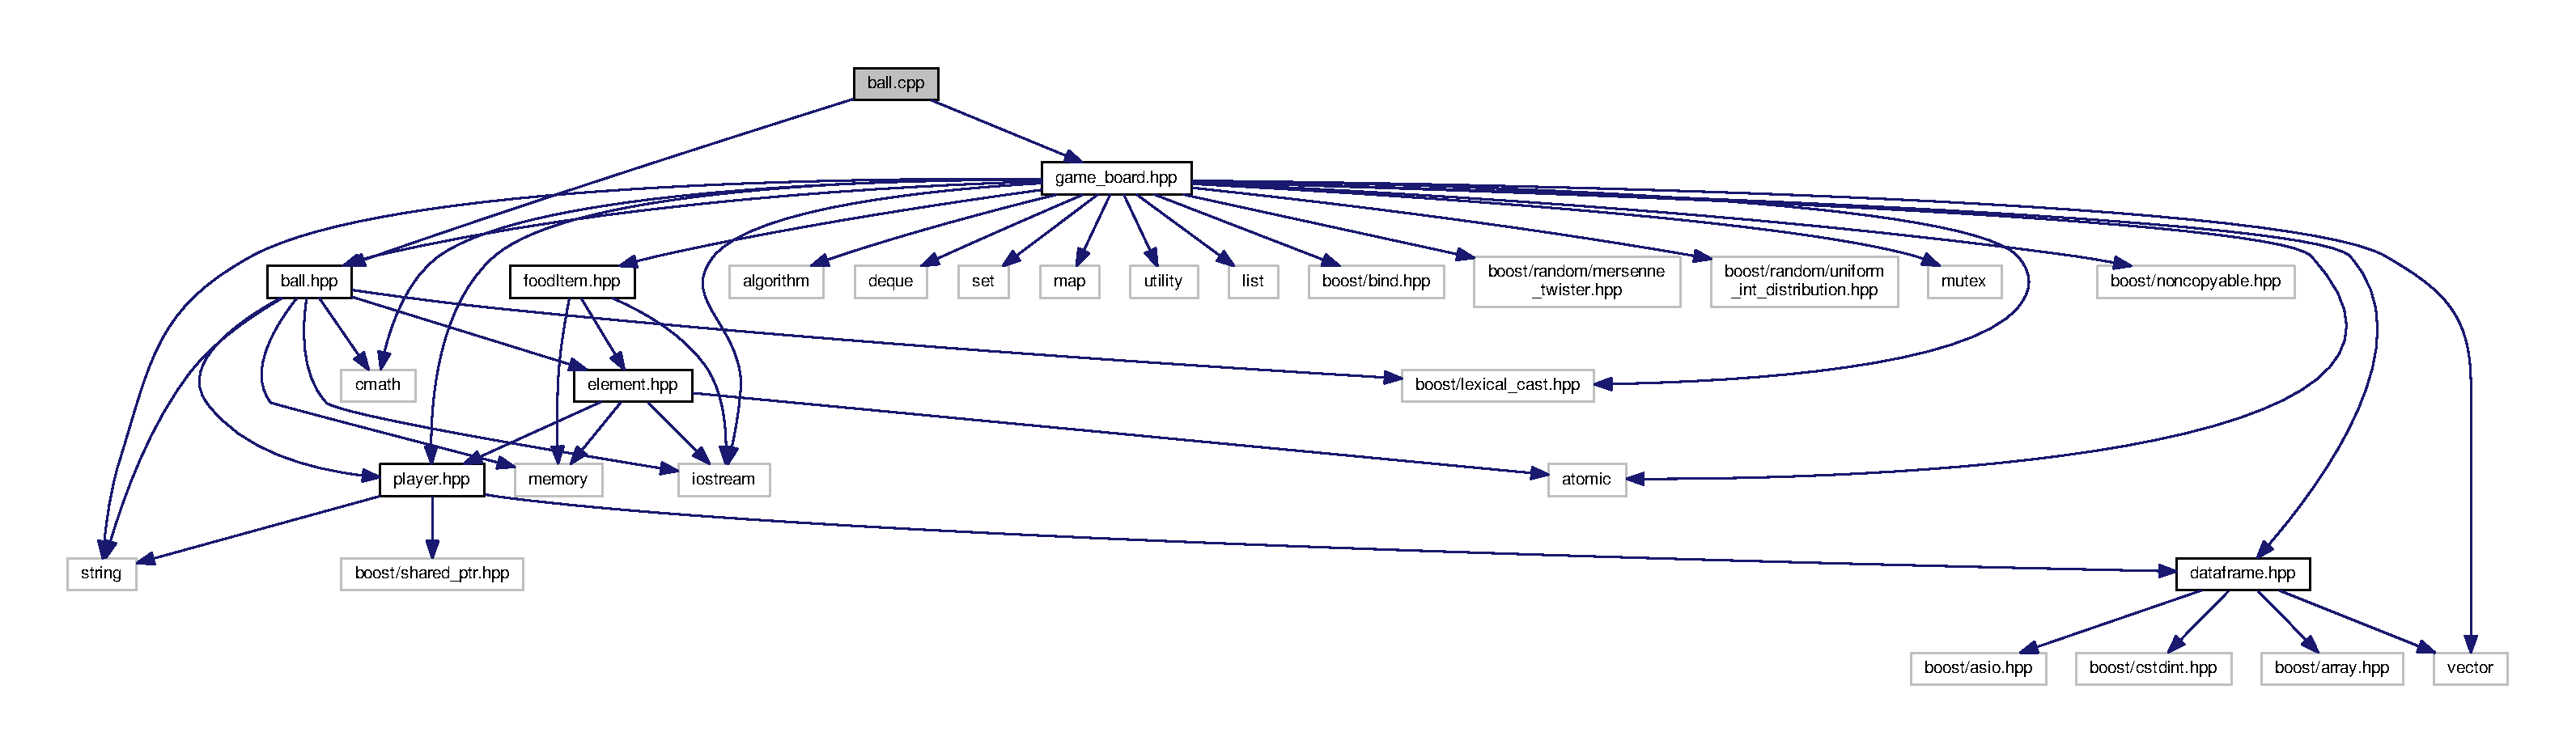
\includegraphics[width=350pt]{ball_8cpp__incl}
\end{center}
\end{figure}
\subsection*{Namespaces}
\begin{DoxyCompactItemize}
\item 
 \hyperlink{namespacewebsocket}{websocket}
\end{DoxyCompactItemize}

\hypertarget{ball_8hpp}{}\section{ball.\+hpp File Reference}
\label{ball_8hpp}\index{ball.\+hpp@{ball.\+hpp}}
{\ttfamily \#include $<$memory$>$}\\*
{\ttfamily \#include $<$iostream$>$}\\*
{\ttfamily \#include $<$string$>$}\\*
{\ttfamily \#include $<$boost/lexical\+\_\+cast.\+hpp$>$}\\*
{\ttfamily \#include $<$cmath$>$}\\*
{\ttfamily \#include \char`\"{}element.\+hpp\char`\"{}}\\*
{\ttfamily \#include \char`\"{}player.\+hpp\char`\"{}}\\*
Include dependency graph for ball.\+hpp\+:\nopagebreak
\begin{figure}[H]
\begin{center}
\leavevmode
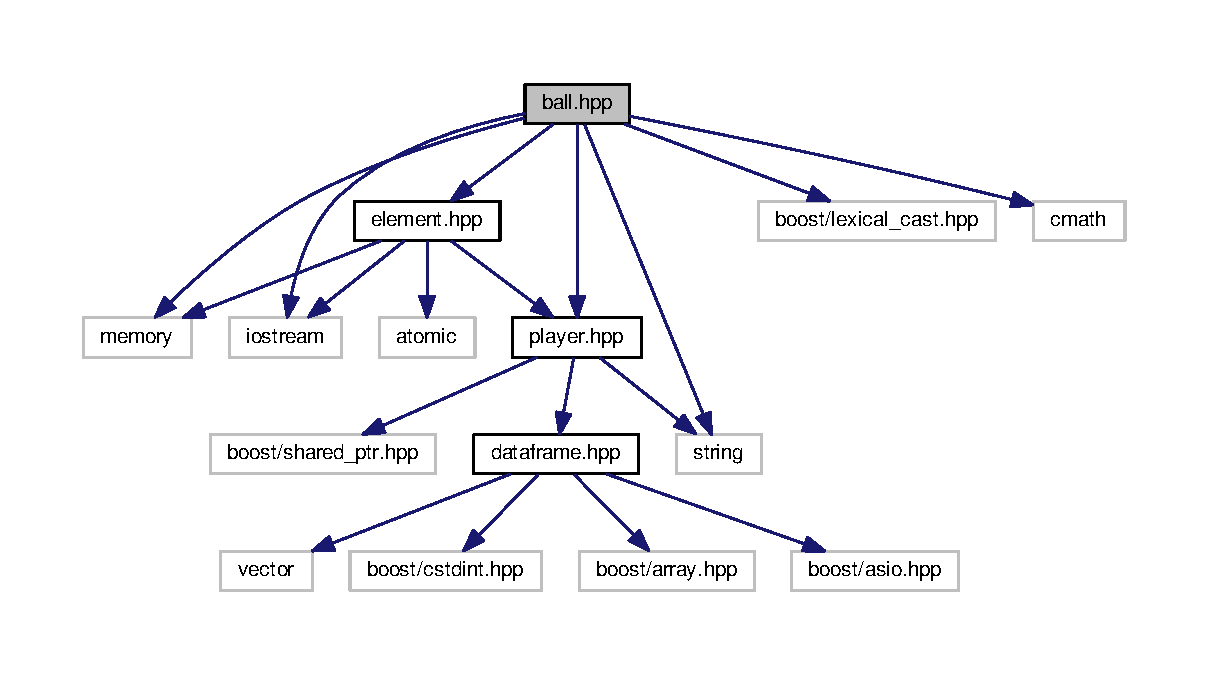
\includegraphics[width=350pt]{ball_8hpp__incl}
\end{center}
\end{figure}
This graph shows which files directly or indirectly include this file\+:\nopagebreak
\begin{figure}[H]
\begin{center}
\leavevmode
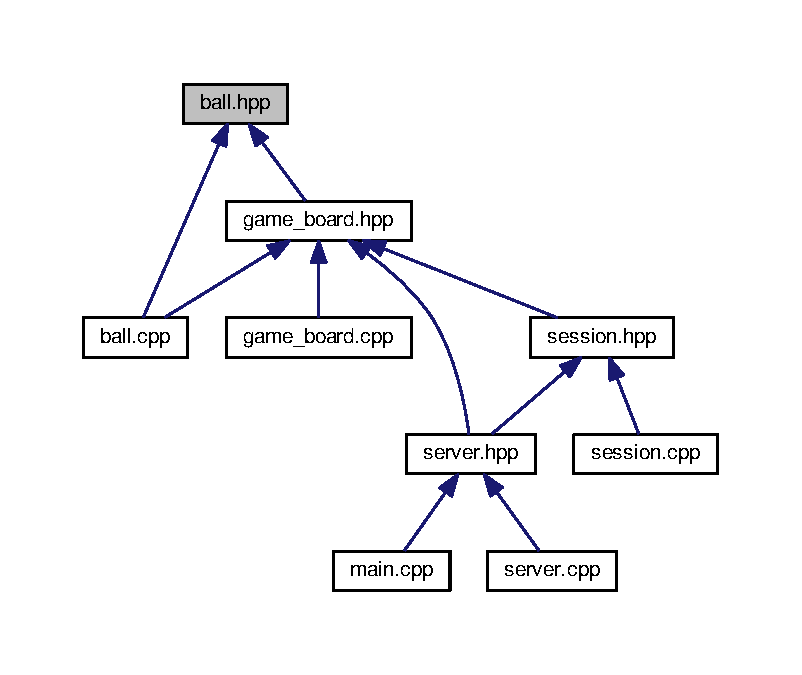
\includegraphics[width=350pt]{ball_8hpp__dep__incl}
\end{center}
\end{figure}
\subsection*{Classes}
\begin{DoxyCompactItemize}
\item 
class \hyperlink{classwebsocket_1_1Ball}{websocket\+::\+Ball}
\end{DoxyCompactItemize}
\subsection*{Namespaces}
\begin{DoxyCompactItemize}
\item 
 \hyperlink{namespacewebsocket}{websocket}
\end{DoxyCompactItemize}
\subsection*{Typedefs}
\begin{DoxyCompactItemize}
\item 
typedef std\+::shared\+\_\+ptr$<$ Ball $>$ \hyperlink{namespacewebsocket_aae1d9cf317a0fb0b83bdfc2f92df77c7}{websocket\+::ball\+\_\+ptr}
\end{DoxyCompactItemize}


\subsection{Detailed Description}
\begin{DoxyAuthor}{Author}
Wojciech Przybysz, Kajetan Spionek Class representing ball owned by a player. 
\end{DoxyAuthor}

\hypertarget{dataframe_8cpp}{}\section{dataframe.\+cpp File Reference}
\label{dataframe_8cpp}\index{dataframe.\+cpp@{dataframe.\+cpp}}
{\ttfamily \#include \char`\"{}dataframe.\+hpp\char`\"{}}\\*
{\ttfamily \#include \char`\"{}dataframe\+\_\+parser.\+hpp\char`\"{}}\\*
Include dependency graph for dataframe.\+cpp\+:\nopagebreak
\begin{figure}[H]
\begin{center}
\leavevmode
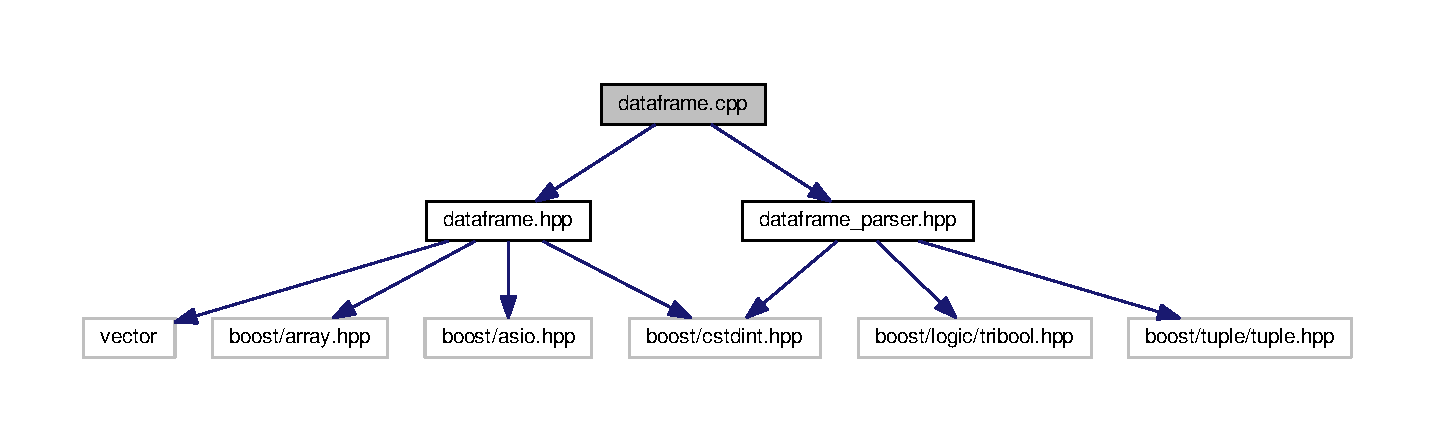
\includegraphics[width=350pt]{dataframe_8cpp__incl}
\end{center}
\end{figure}
\subsection*{Namespaces}
\begin{DoxyCompactItemize}
\item 
 \hyperlink{namespacewebsocket}{websocket}
\end{DoxyCompactItemize}

\hypertarget{dataframe_8hpp}{}\section{dataframe.\+hpp File Reference}
\label{dataframe_8hpp}\index{dataframe.\+hpp@{dataframe.\+hpp}}
{\ttfamily \#include $<$vector$>$}\\*
{\ttfamily \#include $<$boost/cstdint.\+hpp$>$}\\*
{\ttfamily \#include $<$boost/array.\+hpp$>$}\\*
{\ttfamily \#include $<$boost/asio.\+hpp$>$}\\*
Include dependency graph for dataframe.\+hpp\+:\nopagebreak
\begin{figure}[H]
\begin{center}
\leavevmode
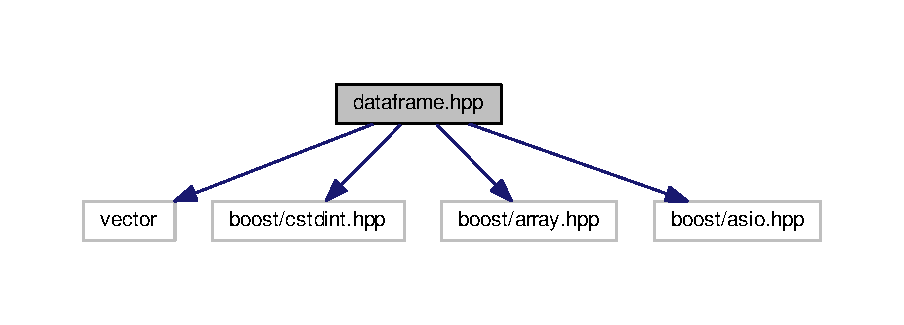
\includegraphics[width=350pt]{dataframe_8hpp__incl}
\end{center}
\end{figure}
This graph shows which files directly or indirectly include this file\+:\nopagebreak
\begin{figure}[H]
\begin{center}
\leavevmode
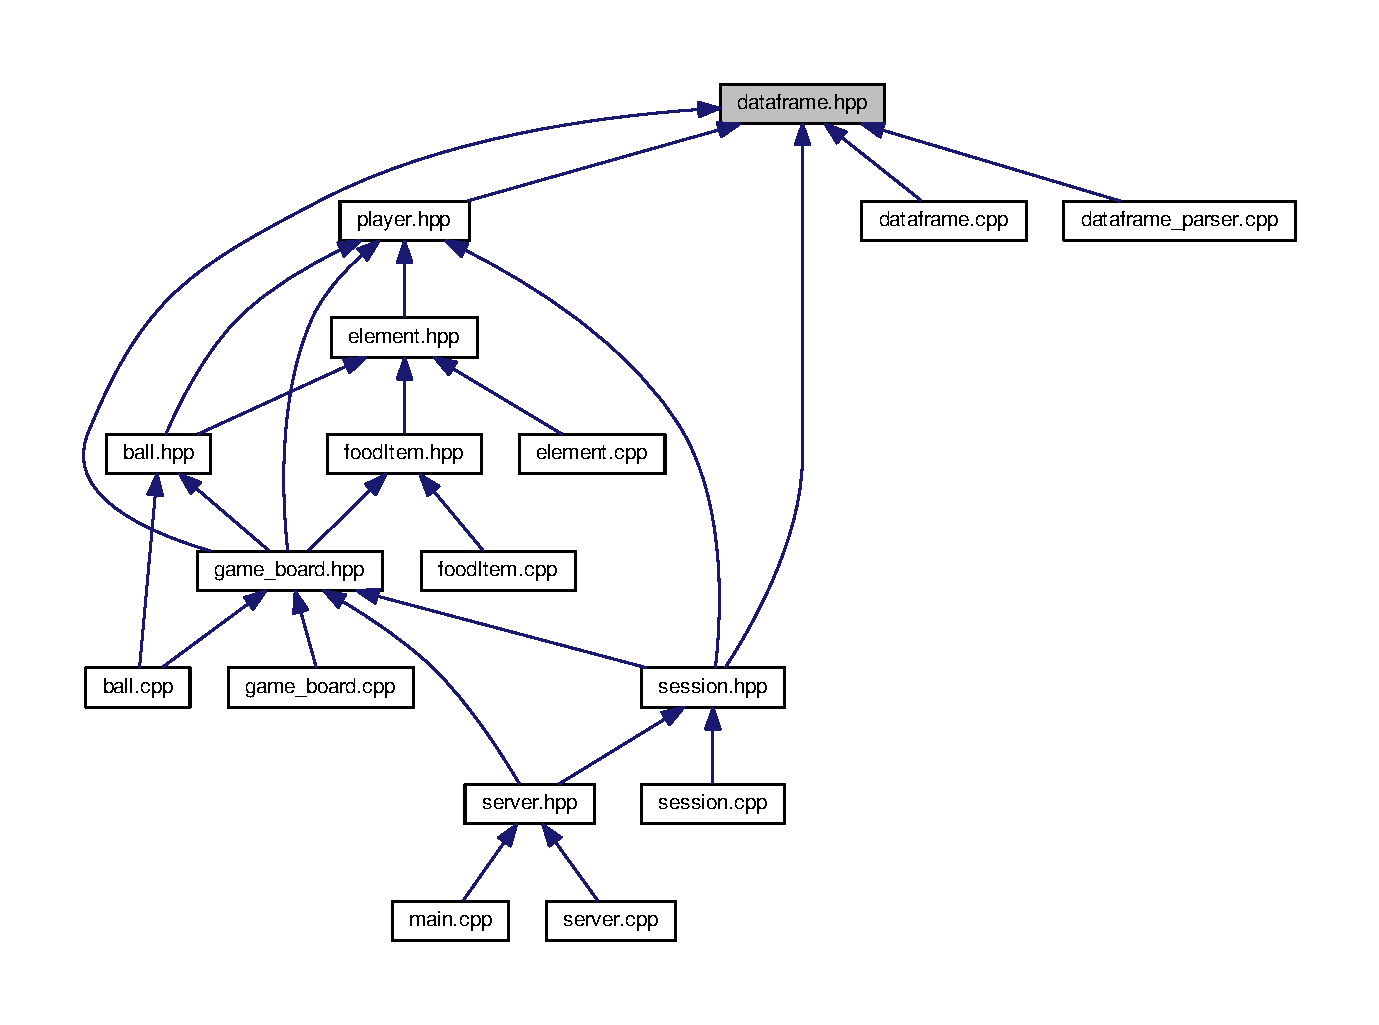
\includegraphics[width=350pt]{dataframe_8hpp__dep__incl}
\end{center}
\end{figure}
\subsection*{Classes}
\begin{DoxyCompactItemize}
\item 
struct \hyperlink{structwebsocket_1_1Dataframe}{websocket\+::\+Dataframe}
\end{DoxyCompactItemize}
\subsection*{Namespaces}
\begin{DoxyCompactItemize}
\item 
 \hyperlink{namespacewebsocket}{websocket}
\end{DoxyCompactItemize}


\subsection{Detailed Description}
\begin{DoxyAuthor}{Author}
A structure to hold websocket frame data. 
\end{DoxyAuthor}

\hypertarget{dataframe__parser_8cpp}{}\section{dataframe\+\_\+parser.\+cpp File Reference}
\label{dataframe__parser_8cpp}\index{dataframe\+\_\+parser.\+cpp@{dataframe\+\_\+parser.\+cpp}}
{\ttfamily \#include \char`\"{}dataframe\+\_\+parser.\+hpp\char`\"{}}\\*
{\ttfamily \#include \char`\"{}dataframe.\+hpp\char`\"{}}\\*
Include dependency graph for dataframe\+\_\+parser.\+cpp\+:\nopagebreak
\begin{figure}[H]
\begin{center}
\leavevmode
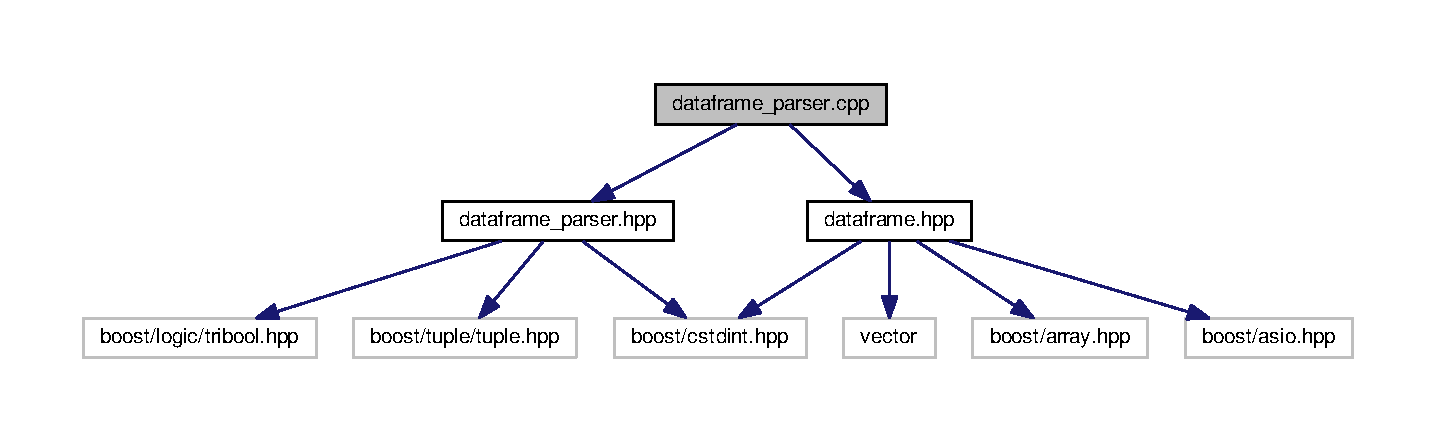
\includegraphics[width=350pt]{dataframe__parser_8cpp__incl}
\end{center}
\end{figure}
\subsection*{Namespaces}
\begin{DoxyCompactItemize}
\item 
 \hyperlink{namespacewebsocket}{websocket}
\end{DoxyCompactItemize}

\hypertarget{dataframe__parser_8hpp}{}\section{dataframe\+\_\+parser.\+hpp File Reference}
\label{dataframe__parser_8hpp}\index{dataframe\+\_\+parser.\+hpp@{dataframe\+\_\+parser.\+hpp}}
{\ttfamily \#include $<$boost/cstdint.\+hpp$>$}\\*
{\ttfamily \#include $<$boost/logic/tribool.\+hpp$>$}\\*
{\ttfamily \#include $<$boost/tuple/tuple.\+hpp$>$}\\*
Include dependency graph for dataframe\+\_\+parser.\+hpp\+:\nopagebreak
\begin{figure}[H]
\begin{center}
\leavevmode
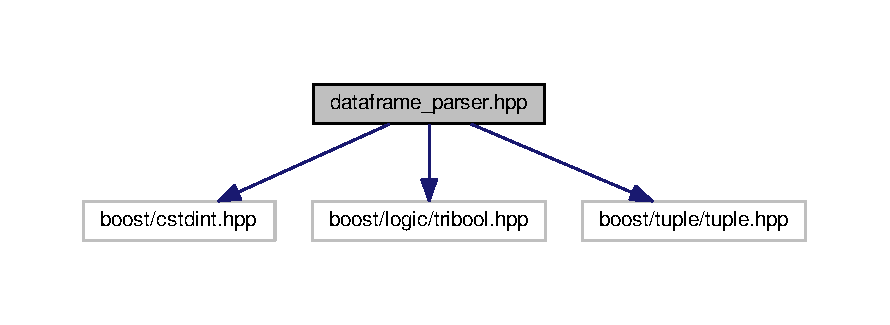
\includegraphics[width=350pt]{dataframe__parser_8hpp__incl}
\end{center}
\end{figure}
This graph shows which files directly or indirectly include this file\+:\nopagebreak
\begin{figure}[H]
\begin{center}
\leavevmode
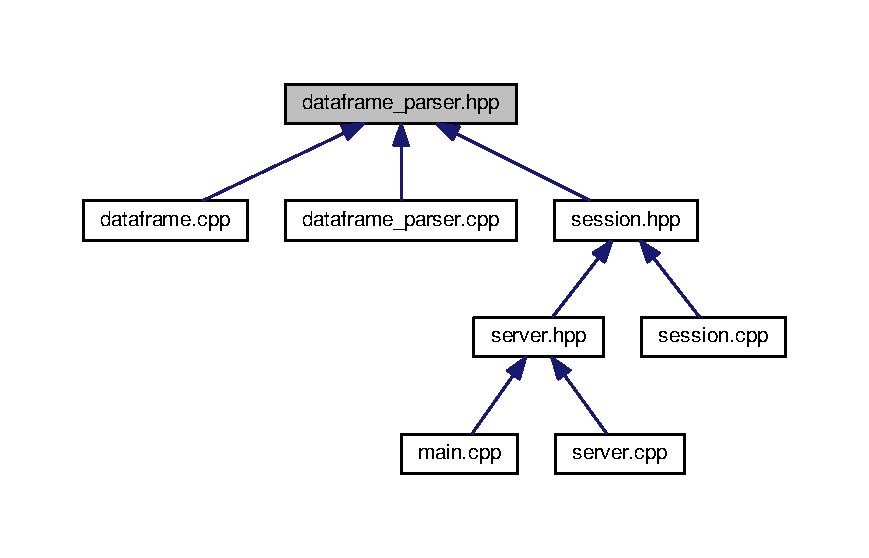
\includegraphics[width=350pt]{dataframe__parser_8hpp__dep__incl}
\end{center}
\end{figure}
\subsection*{Classes}
\begin{DoxyCompactItemize}
\item 
class \hyperlink{classwebsocket_1_1DataframeParser}{websocket\+::\+Dataframe\+Parser}
\end{DoxyCompactItemize}
\subsection*{Namespaces}
\begin{DoxyCompactItemize}
\item 
 \hyperlink{namespacewebsocket}{websocket}
\end{DoxyCompactItemize}


\subsection{Detailed Description}
\begin{DoxyAuthor}{Author}
Parser for incoming dataframes. 
\end{DoxyAuthor}

\hypertarget{element_8cpp}{}\section{element.\+cpp File Reference}
\label{element_8cpp}\index{element.\+cpp@{element.\+cpp}}
{\ttfamily \#include \char`\"{}element.\+hpp\char`\"{}}\\*
Include dependency graph for element.\+cpp\+:
\nopagebreak
\begin{figure}[H]
\begin{center}
\leavevmode
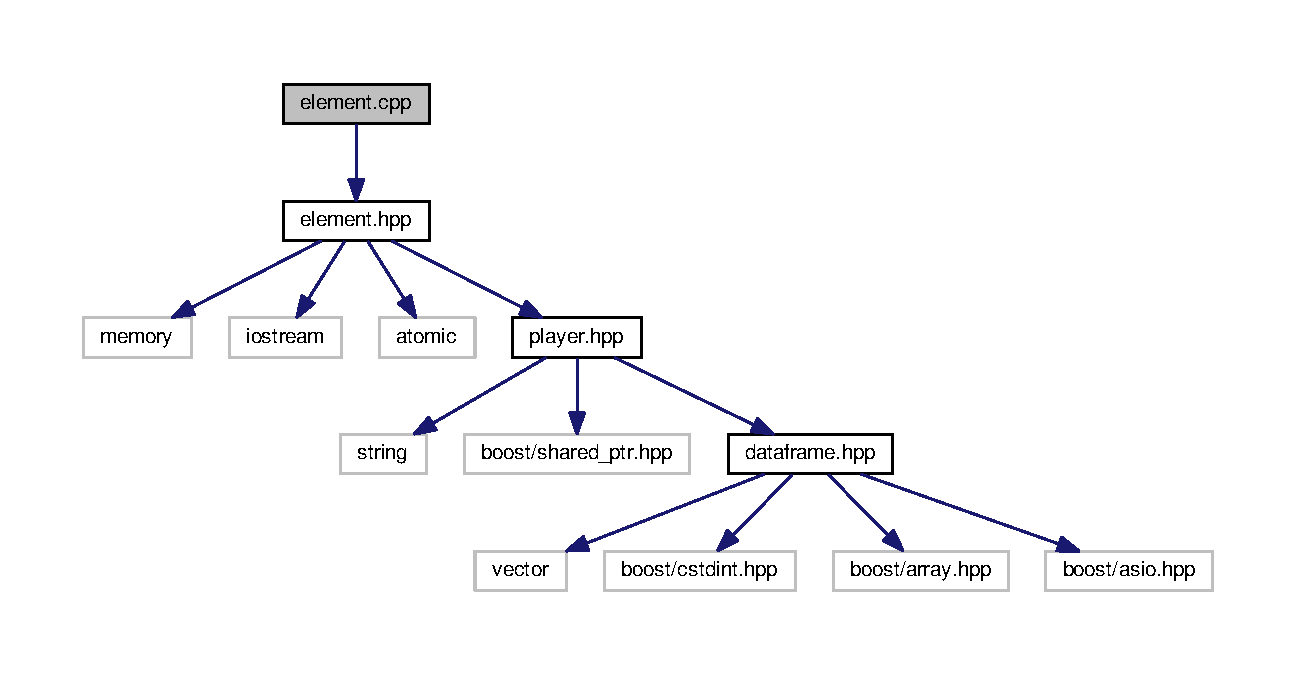
\includegraphics[width=350pt]{element_8cpp__incl}
\end{center}
\end{figure}
\subsection*{Namespaces}
\begin{DoxyCompactItemize}
\item 
 \hyperlink{namespacewebsocket}{websocket}
\end{DoxyCompactItemize}

\hypertarget{element_8hpp}{}\section{element.\+hpp File Reference}
\label{element_8hpp}\index{element.\+hpp@{element.\+hpp}}
{\ttfamily \#include $<$memory$>$}\\*
{\ttfamily \#include $<$iostream$>$}\\*
{\ttfamily \#include $<$atomic$>$}\\*
{\ttfamily \#include \char`\"{}player.\+hpp\char`\"{}}\\*
Include dependency graph for element.\+hpp\+:\nopagebreak
\begin{figure}[H]
\begin{center}
\leavevmode
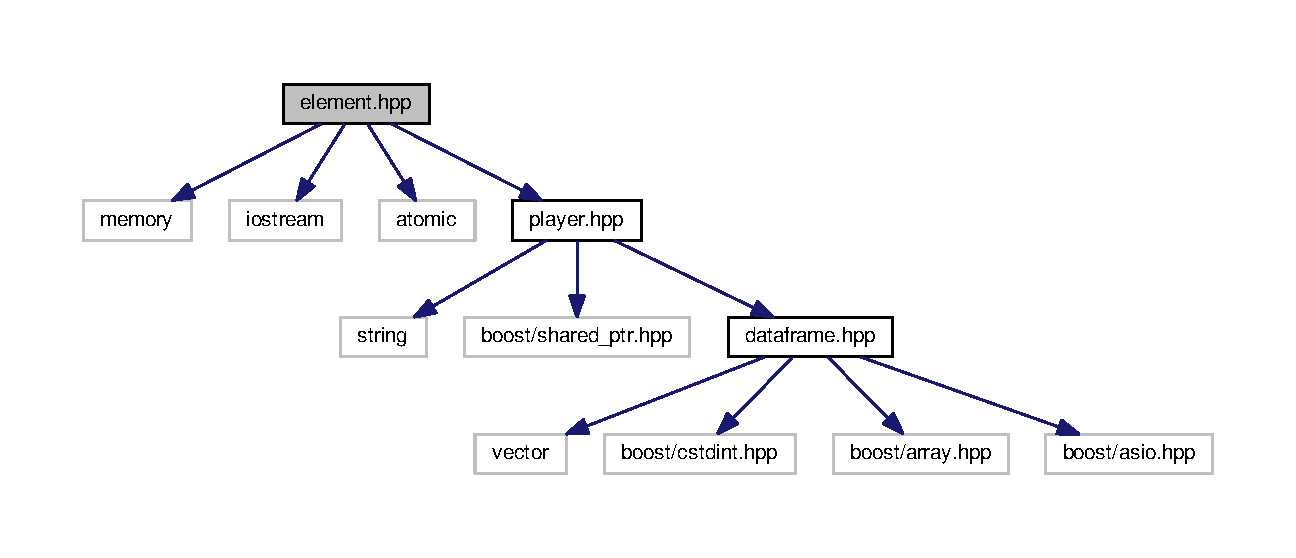
\includegraphics[width=350pt]{element_8hpp__incl}
\end{center}
\end{figure}
This graph shows which files directly or indirectly include this file\+:\nopagebreak
\begin{figure}[H]
\begin{center}
\leavevmode
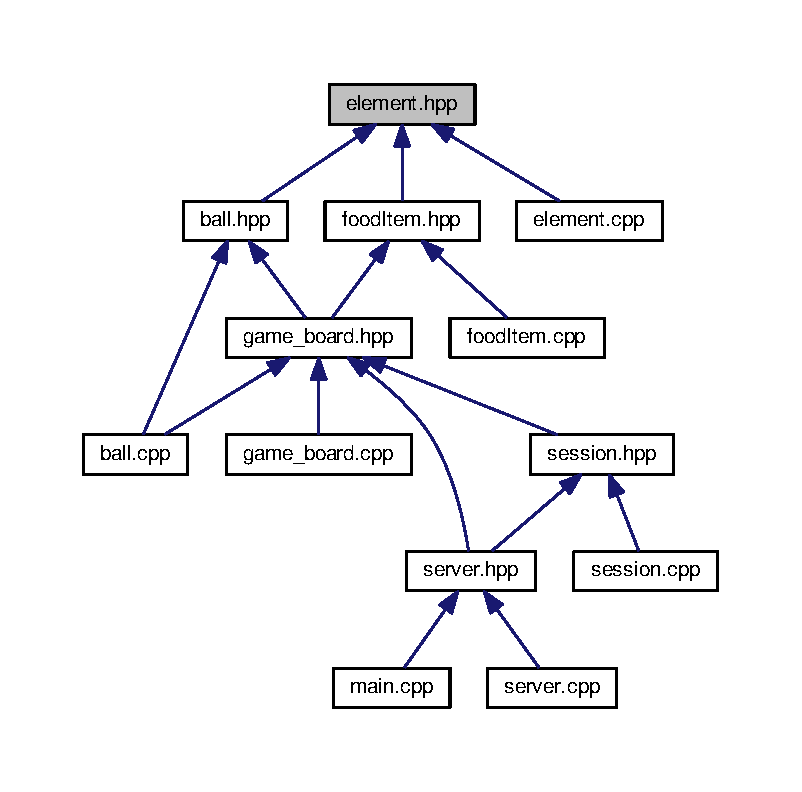
\includegraphics[width=350pt]{element_8hpp__dep__incl}
\end{center}
\end{figure}
\subsection*{Classes}
\begin{DoxyCompactItemize}
\item 
class \hyperlink{classwebsocket_1_1Element}{websocket\+::\+Element}
\end{DoxyCompactItemize}
\subsection*{Namespaces}
\begin{DoxyCompactItemize}
\item 
 \hyperlink{namespacewebsocket}{websocket}
\end{DoxyCompactItemize}
\subsection*{Typedefs}
\begin{DoxyCompactItemize}
\item 
typedef std\+::shared\+\_\+ptr$<$ Element $>$ \hyperlink{namespacewebsocket_a1f36ba91b301b228fa9e9f812883050c}{websocket\+::element\+\_\+ptr}
\end{DoxyCompactItemize}


\subsection{Detailed Description}
\begin{DoxyAuthor}{Author}
Wojciech Przybysz, Kajetan Spionek 
\end{DoxyAuthor}

\hypertarget{foodItem_8cpp}{}\section{food\+Item.\+cpp File Reference}
\label{foodItem_8cpp}\index{food\+Item.\+cpp@{food\+Item.\+cpp}}
{\ttfamily \#include \char`\"{}food\+Item.\+hpp\char`\"{}}\\*
Include dependency graph for food\+Item.\+cpp\+:
\nopagebreak
\begin{figure}[H]
\begin{center}
\leavevmode
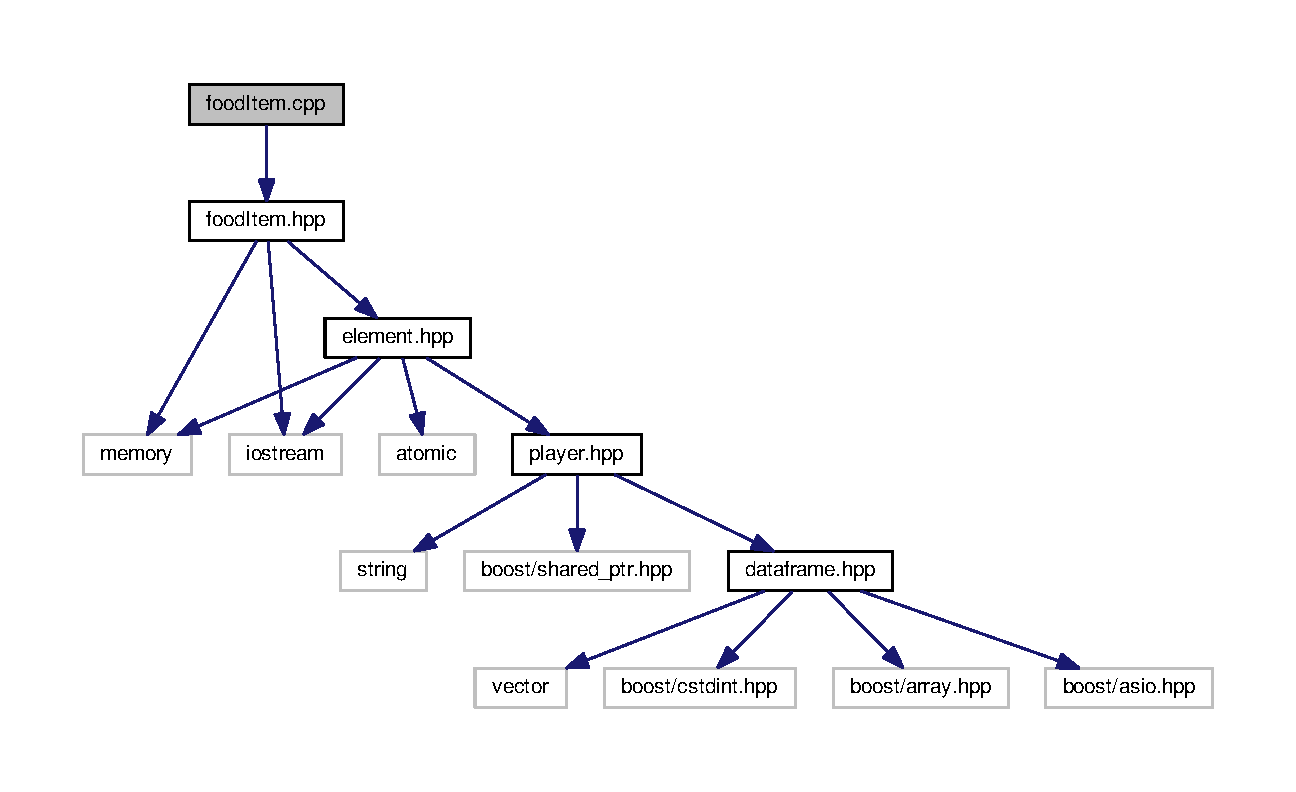
\includegraphics[width=350pt]{foodItem_8cpp__incl}
\end{center}
\end{figure}
\subsection*{Namespaces}
\begin{DoxyCompactItemize}
\item 
 \hyperlink{namespacewebsocket}{websocket}
\end{DoxyCompactItemize}

\hypertarget{foodItem_8hpp}{}\section{food\+Item.\+hpp File Reference}
\label{foodItem_8hpp}\index{food\+Item.\+hpp@{food\+Item.\+hpp}}
{\ttfamily \#include $<$memory$>$}\\*
{\ttfamily \#include $<$iostream$>$}\\*
{\ttfamily \#include \char`\"{}element.\+hpp\char`\"{}}\\*
Include dependency graph for food\+Item.\+hpp\+:\nopagebreak
\begin{figure}[H]
\begin{center}
\leavevmode
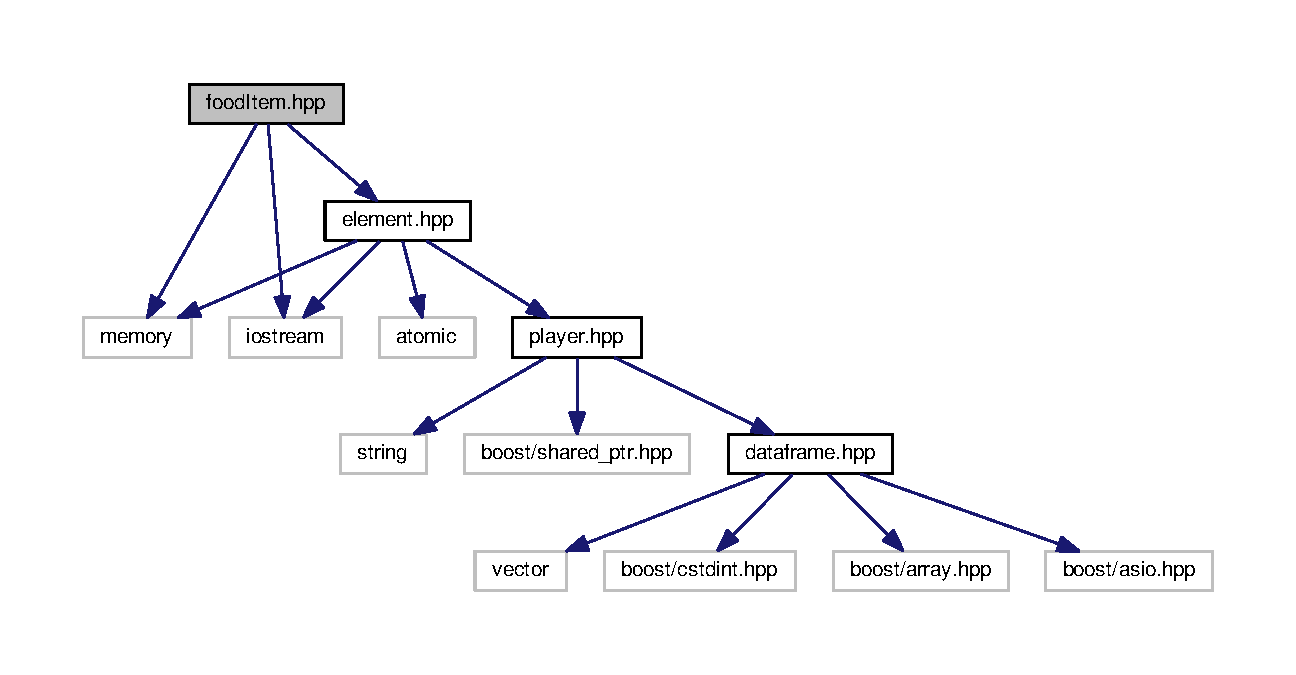
\includegraphics[width=350pt]{foodItem_8hpp__incl}
\end{center}
\end{figure}
This graph shows which files directly or indirectly include this file\+:\nopagebreak
\begin{figure}[H]
\begin{center}
\leavevmode
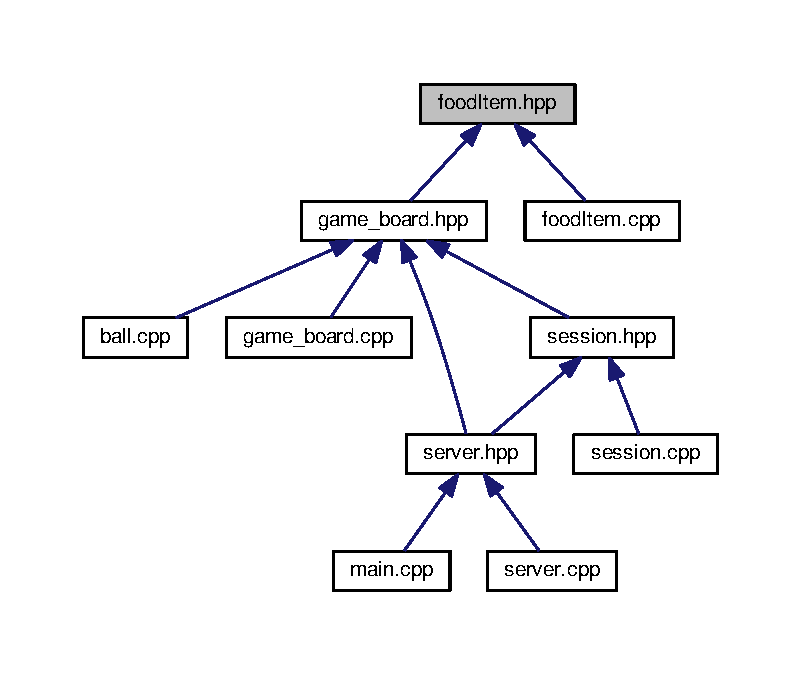
\includegraphics[width=350pt]{foodItem_8hpp__dep__incl}
\end{center}
\end{figure}
\subsection*{Classes}
\begin{DoxyCompactItemize}
\item 
class \hyperlink{classwebsocket_1_1FoodItem}{websocket\+::\+Food\+Item}
\end{DoxyCompactItemize}
\subsection*{Namespaces}
\begin{DoxyCompactItemize}
\item 
 \hyperlink{namespacewebsocket}{websocket}
\end{DoxyCompactItemize}
\subsection*{Typedefs}
\begin{DoxyCompactItemize}
\item 
typedef std\+::shared\+\_\+ptr$<$ Food\+Item $>$ \hyperlink{namespacewebsocket_a198017789b8c5fa32315a12d5ce97869}{websocket\+::food\+\_\+ptr}
\end{DoxyCompactItemize}


\subsection{Detailed Description}
\begin{DoxyAuthor}{Author}
Wojciech Przybysz, Kajetan Spionek 
\end{DoxyAuthor}

\hypertarget{game__board_8cpp}{}\section{game\+\_\+board.\+cpp File Reference}
\label{game__board_8cpp}\index{game\+\_\+board.\+cpp@{game\+\_\+board.\+cpp}}
{\ttfamily \#include \char`\"{}game\+\_\+board.\+hpp\char`\"{}}\\*
Include dependency graph for game\+\_\+board.\+cpp\+:
\nopagebreak
\begin{figure}[H]
\begin{center}
\leavevmode
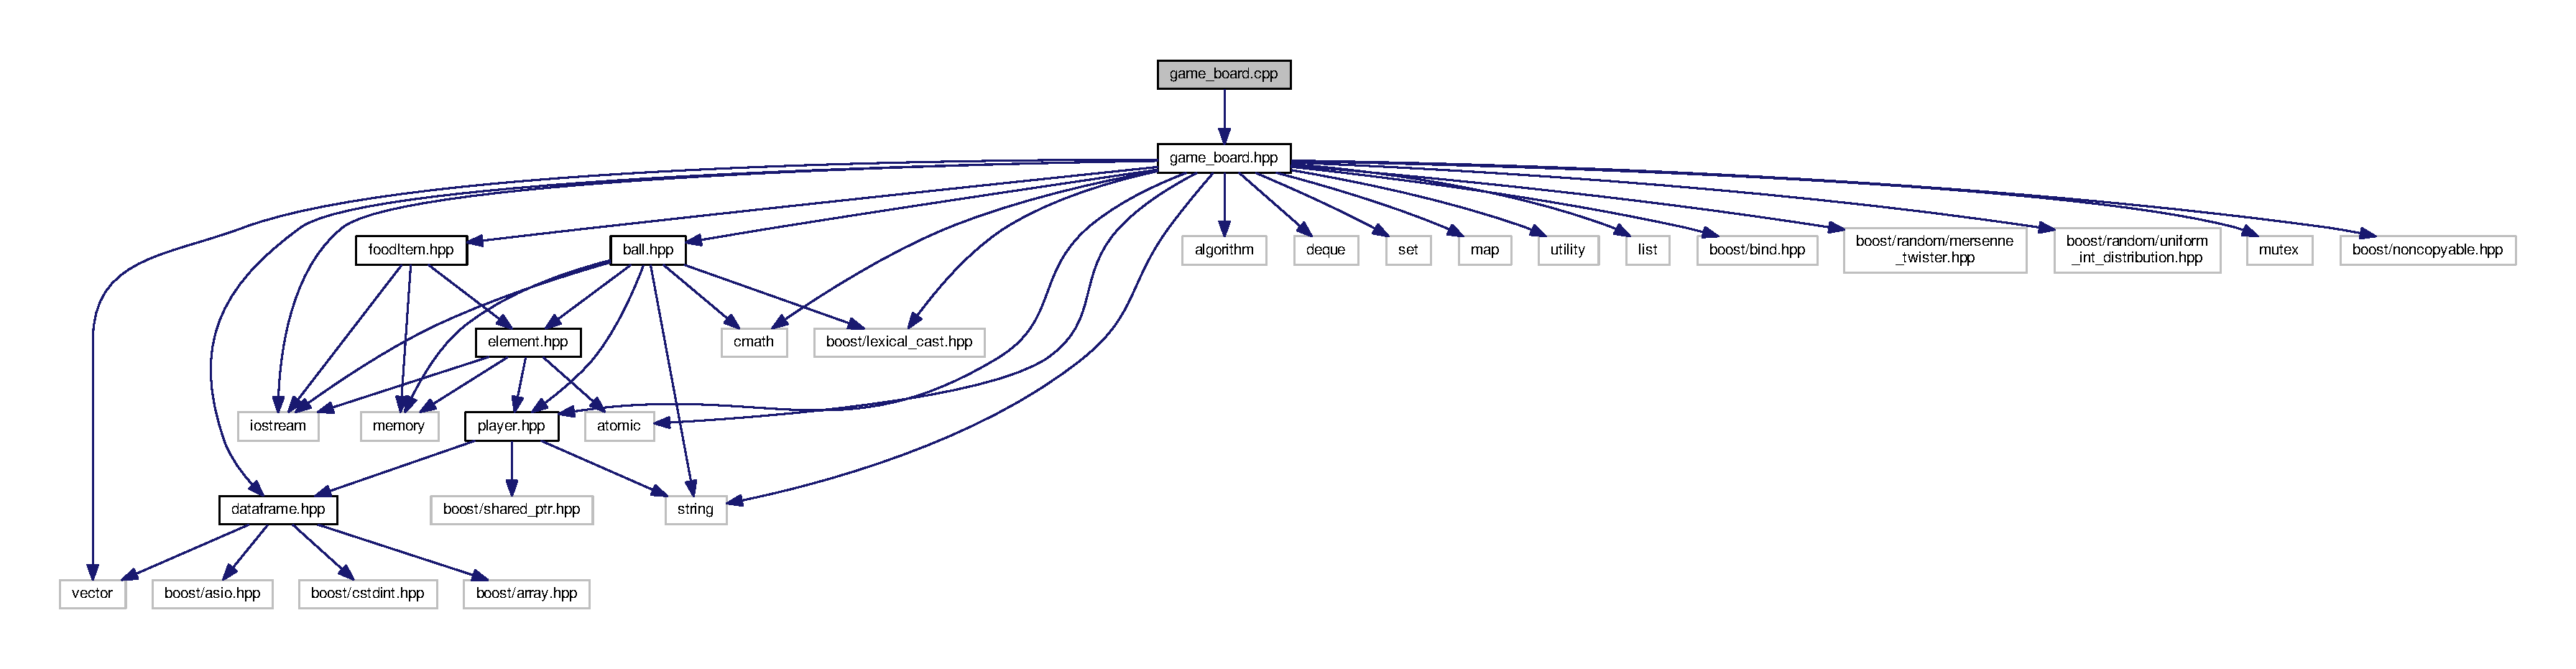
\includegraphics[width=350pt]{game__board_8cpp__incl}
\end{center}
\end{figure}
\subsection*{Namespaces}
\begin{DoxyCompactItemize}
\item 
 \hyperlink{namespacewebsocket}{websocket}
\end{DoxyCompactItemize}

\hypertarget{game__board_8hpp}{}\section{game\+\_\+board.\+hpp File Reference}
\label{game__board_8hpp}\index{game\+\_\+board.\+hpp@{game\+\_\+board.\+hpp}}
{\ttfamily \#include $<$string$>$}\\*
{\ttfamily \#include $<$algorithm$>$}\\*
{\ttfamily \#include $<$deque$>$}\\*
{\ttfamily \#include $<$set$>$}\\*
{\ttfamily \#include $<$map$>$}\\*
{\ttfamily \#include $<$utility$>$}\\*
{\ttfamily \#include $<$list$>$}\\*
{\ttfamily \#include $<$vector$>$}\\*
{\ttfamily \#include $<$iostream$>$}\\*
{\ttfamily \#include $<$cmath$>$}\\*
{\ttfamily \#include $<$atomic$>$}\\*
{\ttfamily \#include $<$boost/lexical\+\_\+cast.\+hpp$>$}\\*
{\ttfamily \#include $<$boost/bind.\+hpp$>$}\\*
{\ttfamily \#include $<$boost/random/mersenne\+\_\+twister.\+hpp$>$}\\*
{\ttfamily \#include $<$boost/random/uniform\+\_\+int\+\_\+distribution.\+hpp$>$}\\*
{\ttfamily \#include $<$mutex$>$}\\*
{\ttfamily \#include \char`\"{}dataframe.\+hpp\char`\"{}}\\*
{\ttfamily \#include \char`\"{}player.\+hpp\char`\"{}}\\*
{\ttfamily \#include \char`\"{}food\+Item.\+hpp\char`\"{}}\\*
{\ttfamily \#include \char`\"{}ball.\+hpp\char`\"{}}\\*
{\ttfamily \#include $<$boost/noncopyable.\+hpp$>$}\\*
Include dependency graph for game\+\_\+board.\+hpp\+:
\nopagebreak
\begin{figure}[H]
\begin{center}
\leavevmode
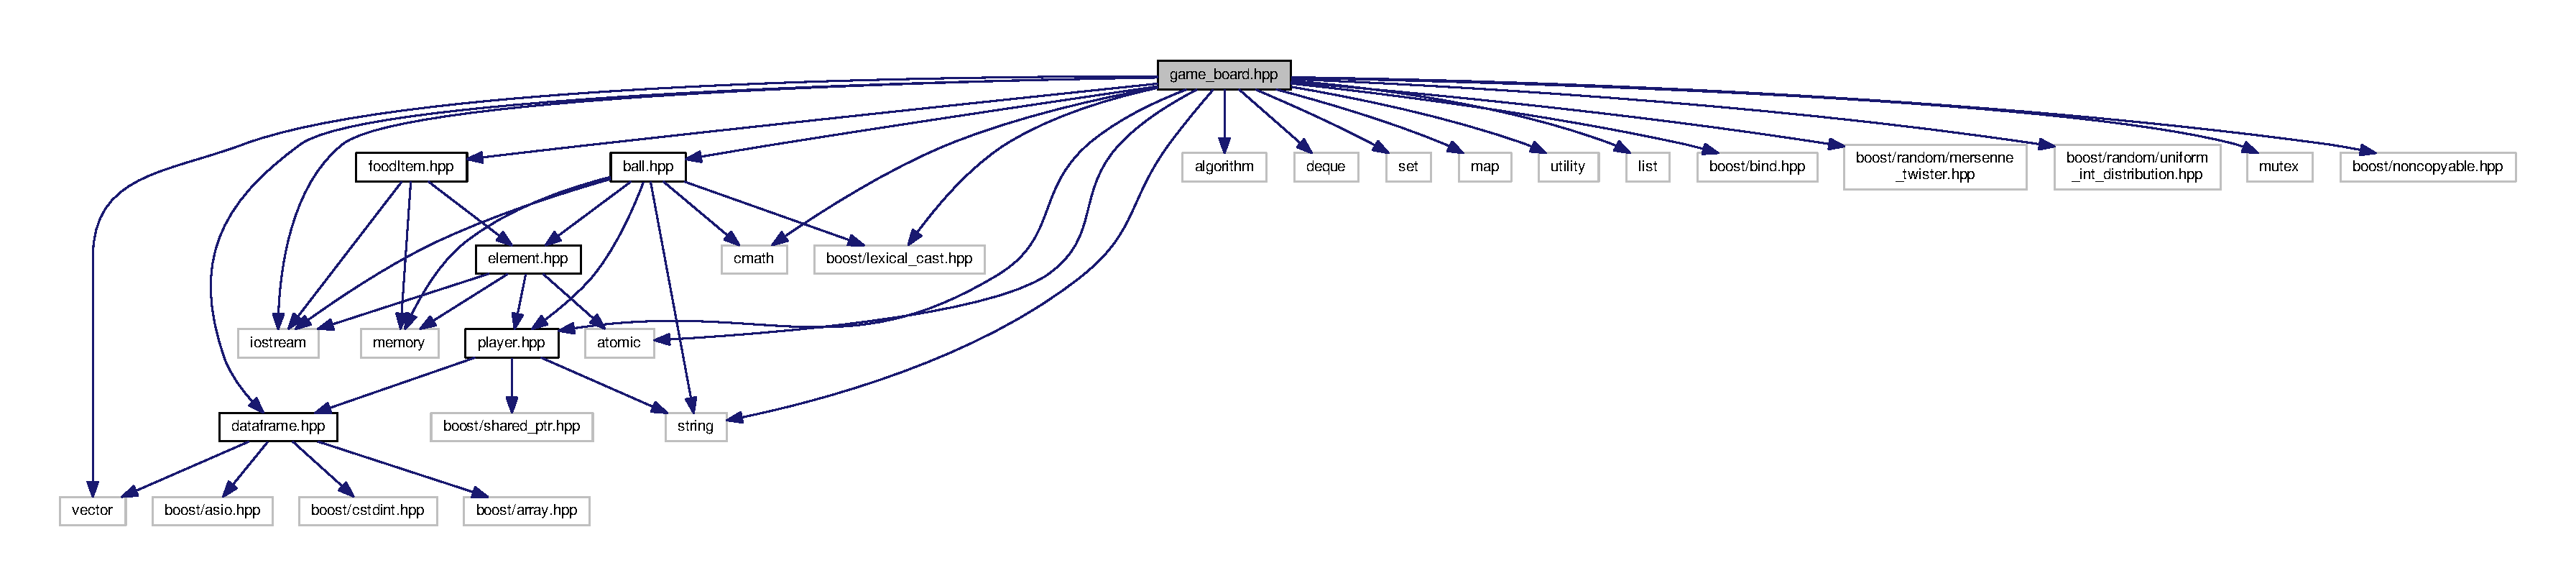
\includegraphics[width=350pt]{game__board_8hpp__incl}
\end{center}
\end{figure}
This graph shows which files directly or indirectly include this file\+:\nopagebreak
\begin{figure}[H]
\begin{center}
\leavevmode
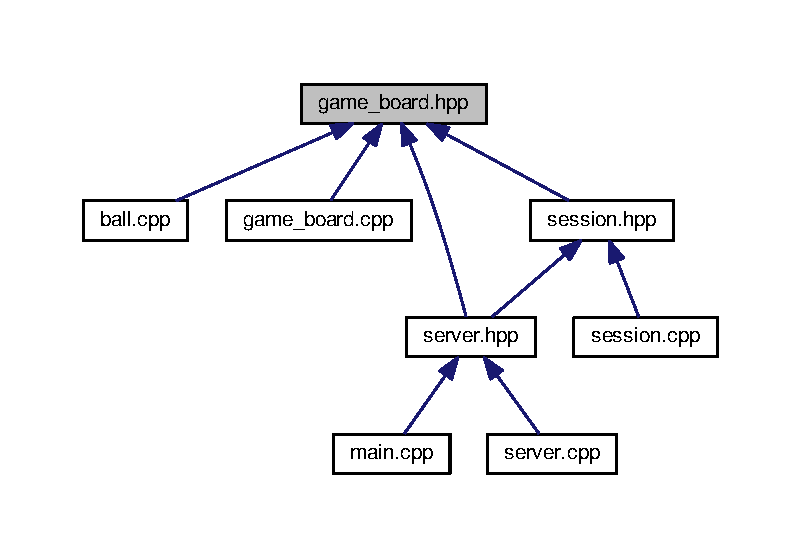
\includegraphics[width=350pt]{game__board_8hpp__dep__incl}
\end{center}
\end{figure}
\subsection*{Classes}
\begin{DoxyCompactItemize}
\item 
class \hyperlink{classwebsocket_1_1GameBoard}{websocket\+::\+Game\+Board}
\end{DoxyCompactItemize}
\subsection*{Namespaces}
\begin{DoxyCompactItemize}
\item 
 \hyperlink{namespacewebsocket}{websocket}
\end{DoxyCompactItemize}
\subsection*{Typedefs}
\begin{DoxyCompactItemize}
\item 
typedef std\+::deque$<$ Dataframe $>$ \hyperlink{namespacewebsocket_ae3fdf29bb367b5baf5be703253a4edfa}{websocket\+::message\+\_\+queue}
\end{DoxyCompactItemize}


\subsection{Detailed Description}
\begin{DoxyAuthor}{Author}
Wojciech Przybysz, Kajetan Spionek 
\end{DoxyAuthor}

\hypertarget{header_8hpp}{}\section{header.\+hpp File Reference}
\label{header_8hpp}\index{header.\+hpp@{header.\+hpp}}
{\ttfamily \#include $<$string$>$}\\*
Include dependency graph for header.\+hpp\+:\nopagebreak
\begin{figure}[H]
\begin{center}
\leavevmode
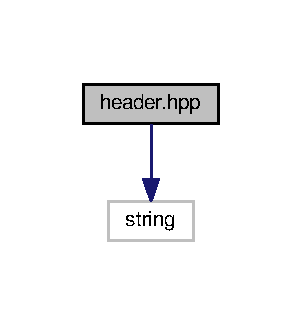
\includegraphics[width=145pt]{header_8hpp__incl}
\end{center}
\end{figure}
This graph shows which files directly or indirectly include this file\+:\nopagebreak
\begin{figure}[H]
\begin{center}
\leavevmode
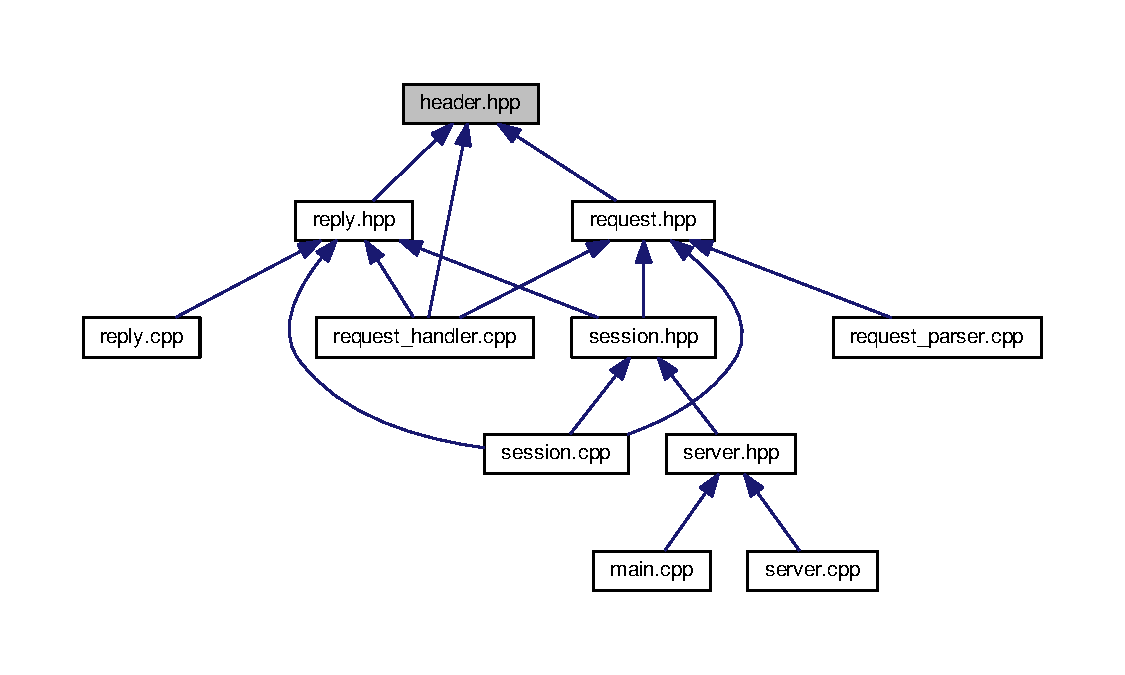
\includegraphics[width=350pt]{header_8hpp__dep__incl}
\end{center}
\end{figure}
\subsection*{Classes}
\begin{DoxyCompactItemize}
\item 
struct \hyperlink{structwebsocket_1_1http_1_1Header}{websocket\+::http\+::\+Header}
\end{DoxyCompactItemize}
\subsection*{Namespaces}
\begin{DoxyCompactItemize}
\item 
 \hyperlink{namespacewebsocket}{websocket}
\item 
 \hyperlink{namespacewebsocket_1_1http}{websocket\+::http}
\end{DoxyCompactItemize}


\subsection{Detailed Description}
\begin{DoxyAuthor}{Author}
Stucture for H\+T\+TP header 
\end{DoxyAuthor}

\hypertarget{main_8cpp}{}\section{main.\+cpp File Reference}
\label{main_8cpp}\index{main.\+cpp@{main.\+cpp}}
{\ttfamily \#include $<$iostream$>$}\\*
{\ttfamily \#include \char`\"{}webserver.\+hpp\char`\"{}}\\*
{\ttfamily \#include \char`\"{}element.\+hpp\char`\"{}}\\*
{\ttfamily \#include \char`\"{}player.\+hpp\char`\"{}}\\*
{\ttfamily \#include \char`\"{}game\+Board.\+hpp\char`\"{}}\\*
Include dependency graph for main.\+cpp\+:
\nopagebreak
\begin{figure}[H]
\begin{center}
\leavevmode
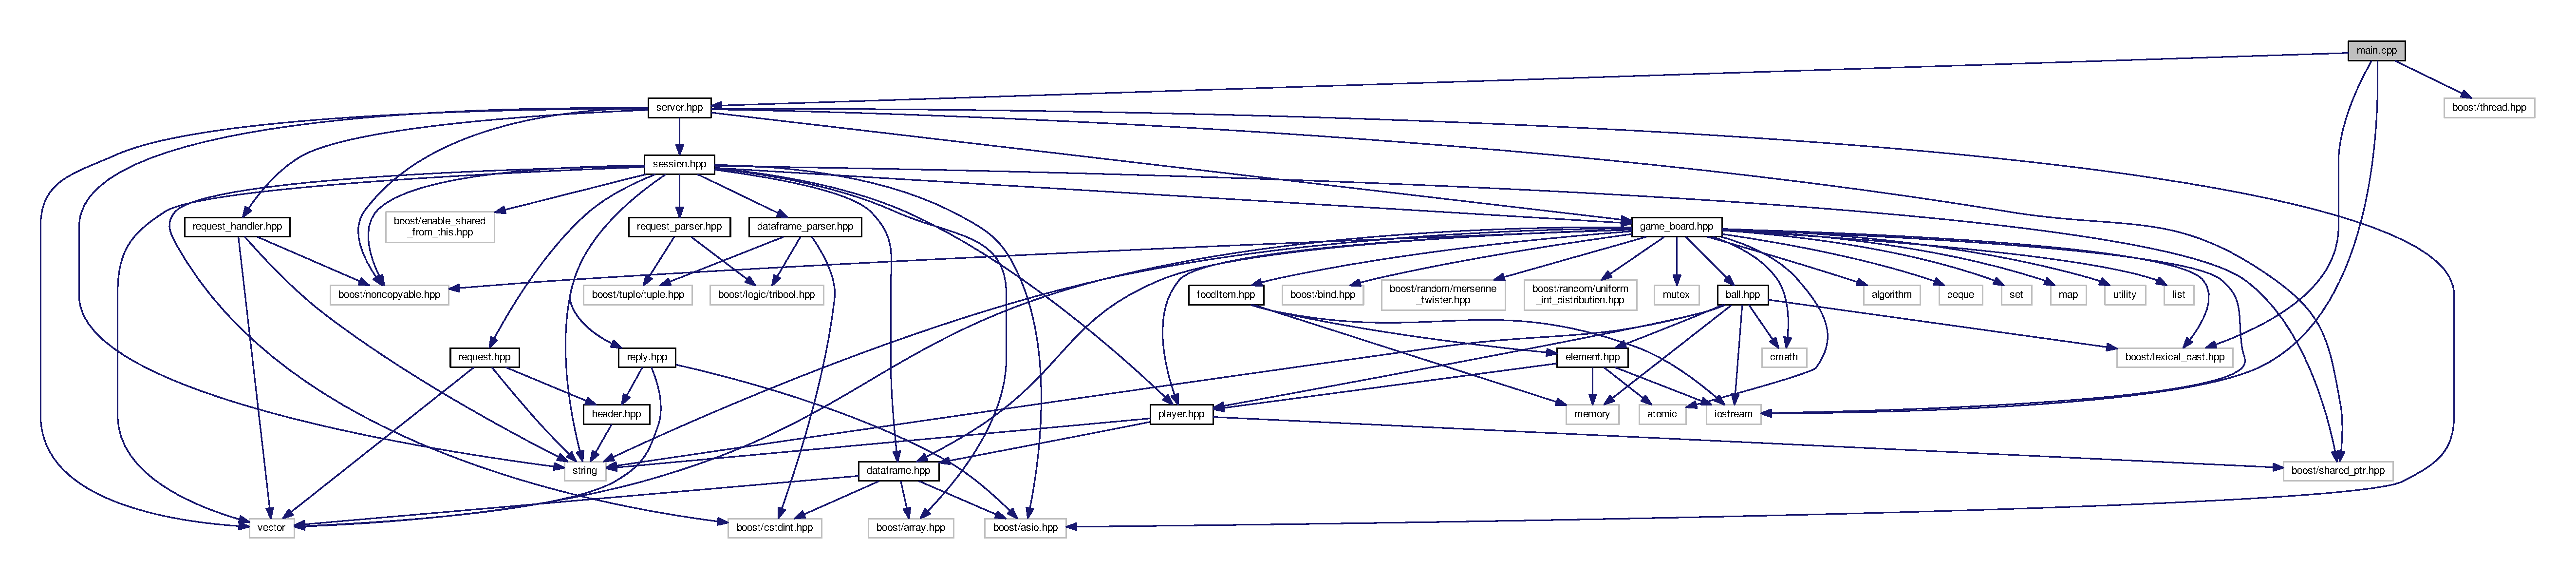
\includegraphics[width=350pt]{main_8cpp__incl}
\end{center}
\end{figure}
\subsection*{Functions}
\begin{DoxyCompactItemize}
\item 
int {\bfseries main} (int argc, char $\ast$argv\mbox{[}$\,$\mbox{]})\hypertarget{main_8cpp_a0ddf1224851353fc92bfbff6f499fa97}{}\label{main_8cpp_a0ddf1224851353fc92bfbff6f499fa97}

\end{DoxyCompactItemize}


\subsection{Detailed Description}
\begin{DoxyAuthor}{Author}

\end{DoxyAuthor}
\begin{DoxyDate}{Date}

\end{DoxyDate}

\hypertarget{player_8hpp}{}\section{player.\+hpp File Reference}
\label{player_8hpp}\index{player.\+hpp@{player.\+hpp}}
{\ttfamily \#include $<$string$>$}\\*
{\ttfamily \#include $<$boost/shared\+\_\+ptr.\+hpp$>$}\\*
{\ttfamily \#include \char`\"{}dataframe.\+hpp\char`\"{}}\\*
Include dependency graph for player.\+hpp\+:\nopagebreak
\begin{figure}[H]
\begin{center}
\leavevmode
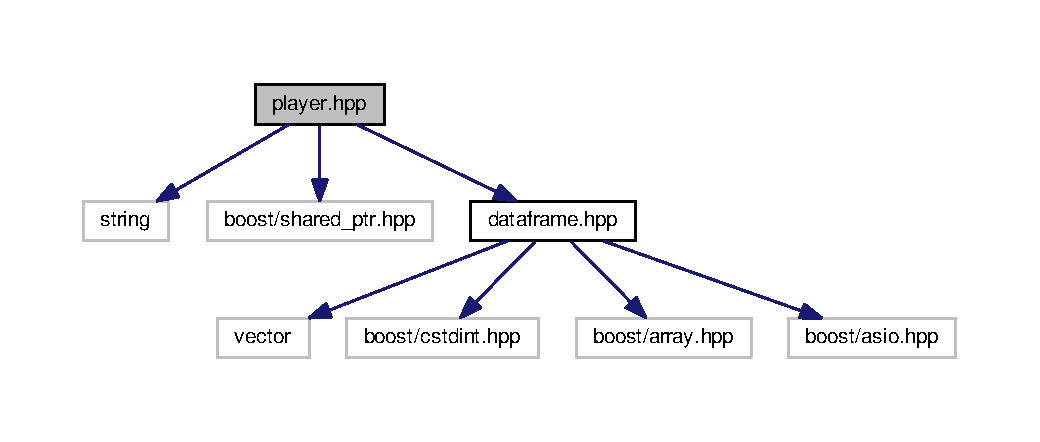
\includegraphics[width=350pt]{player_8hpp__incl}
\end{center}
\end{figure}
This graph shows which files directly or indirectly include this file\+:\nopagebreak
\begin{figure}[H]
\begin{center}
\leavevmode
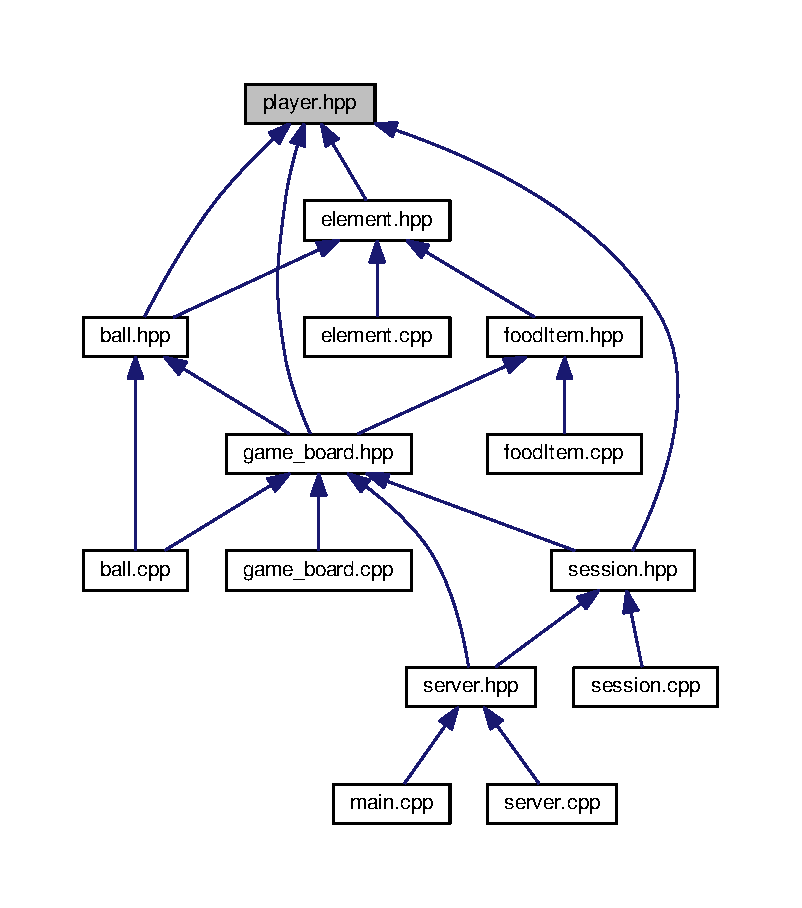
\includegraphics[width=350pt]{player_8hpp__dep__incl}
\end{center}
\end{figure}
\subsection*{Classes}
\begin{DoxyCompactItemize}
\item 
class \hyperlink{classwebsocket_1_1Player}{websocket\+::\+Player}
\end{DoxyCompactItemize}
\subsection*{Namespaces}
\begin{DoxyCompactItemize}
\item 
 \hyperlink{namespacewebsocket}{websocket}
\end{DoxyCompactItemize}
\subsection*{Typedefs}
\begin{DoxyCompactItemize}
\item 
typedef boost\+::shared\+\_\+ptr$<$ Player $>$ \hyperlink{namespacewebsocket_aec8d52893bdf524a1412533a63b006a3}{websocket\+::player\+\_\+ptr}
\end{DoxyCompactItemize}


\subsection{Detailed Description}
\begin{DoxyAuthor}{Author}
Wojciech Przybysz, Kajetan Spionek 
\end{DoxyAuthor}

\hypertarget{reply_8cpp}{}\section{reply.\+cpp File Reference}
\label{reply_8cpp}\index{reply.\+cpp@{reply.\+cpp}}
{\ttfamily \#include \char`\"{}reply.\+hpp\char`\"{}}\\*
{\ttfamily \#include $<$string$>$}\\*
Include dependency graph for reply.\+cpp\+:
\nopagebreak
\begin{figure}[H]
\begin{center}
\leavevmode
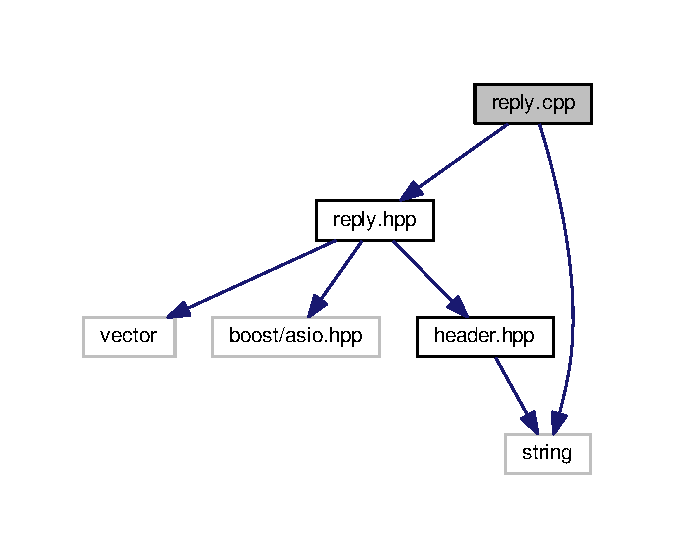
\includegraphics[width=324pt]{reply_8cpp__incl}
\end{center}
\end{figure}
\subsection*{Namespaces}
\begin{DoxyCompactItemize}
\item 
 \hyperlink{namespacewebsocket}{websocket}
\item 
 \hyperlink{namespacewebsocket_1_1http}{websocket\+::http}
\item 
 \hyperlink{namespacewebsocket_1_1http_1_1status__strings}{websocket\+::http\+::status\+\_\+strings}
\item 
 \hyperlink{namespacewebsocket_1_1http_1_1misc__strings}{websocket\+::http\+::misc\+\_\+strings}
\end{DoxyCompactItemize}
\subsection*{Functions}
\begin{DoxyCompactItemize}
\item 
boost\+::asio\+::const\+\_\+buffer \hyperlink{namespacewebsocket_1_1http_1_1status__strings_a71a3c805bd5bbbf577264ca762da4299}{websocket\+::http\+::status\+\_\+strings\+::to\+\_\+buffer} (Reply\+::status\+\_\+type status)
\end{DoxyCompactItemize}
\subsection*{Variables}
\begin{DoxyCompactItemize}
\item 
const std\+::string \hyperlink{namespacewebsocket_1_1http_1_1status__strings_a9b60f1719697fb464b7063cb436e1d75}{websocket\+::http\+::status\+\_\+strings\+::switching\+\_\+protocols}
\item 
const std\+::string \hyperlink{namespacewebsocket_1_1http_1_1status__strings_a29073784a5e6444e93b0925153605222}{websocket\+::http\+::status\+\_\+strings\+::bad\+\_\+request}
\item 
const std\+::string \hyperlink{namespacewebsocket_1_1http_1_1status__strings_a364b430d5e52bc7600da0bcc5dc0d5fc}{websocket\+::http\+::status\+\_\+strings\+::internal\+\_\+server\+\_\+error}
\item 
const char \hyperlink{namespacewebsocket_1_1http_1_1misc__strings_a8fede78f1be63335d445aabd0277727e}{websocket\+::http\+::misc\+\_\+strings\+::name\+\_\+value\+\_\+separator} \mbox{[}$\,$\mbox{]} = \{ \textquotesingle{}\+:\textquotesingle{}, \textquotesingle{} \textquotesingle{} \}
\item 
const char \hyperlink{namespacewebsocket_1_1http_1_1misc__strings_a570bafe7096a0c7904f41f8d6ada54af}{websocket\+::http\+::misc\+\_\+strings\+::crlf} \mbox{[}$\,$\mbox{]} = \{ \textquotesingle{}\textbackslash{}r\textquotesingle{}, \textquotesingle{}\textbackslash{}n\textquotesingle{} \}
\end{DoxyCompactItemize}

\hypertarget{reply_8hpp}{}\section{reply.\+hpp File Reference}
\label{reply_8hpp}\index{reply.\+hpp@{reply.\+hpp}}
{\ttfamily \#include $<$vector$>$}\\*
{\ttfamily \#include $<$boost/asio.\+hpp$>$}\\*
{\ttfamily \#include \char`\"{}header.\+hpp\char`\"{}}\\*
Include dependency graph for reply.\+hpp\+:
\nopagebreak
\begin{figure}[H]
\begin{center}
\leavevmode
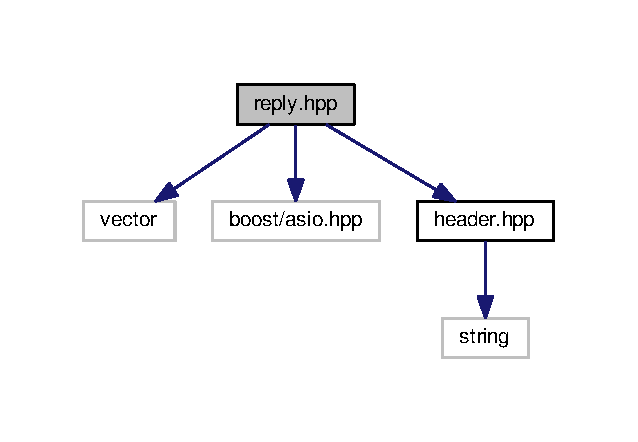
\includegraphics[width=306pt]{reply_8hpp__incl}
\end{center}
\end{figure}
This graph shows which files directly or indirectly include this file\+:
\nopagebreak
\begin{figure}[H]
\begin{center}
\leavevmode
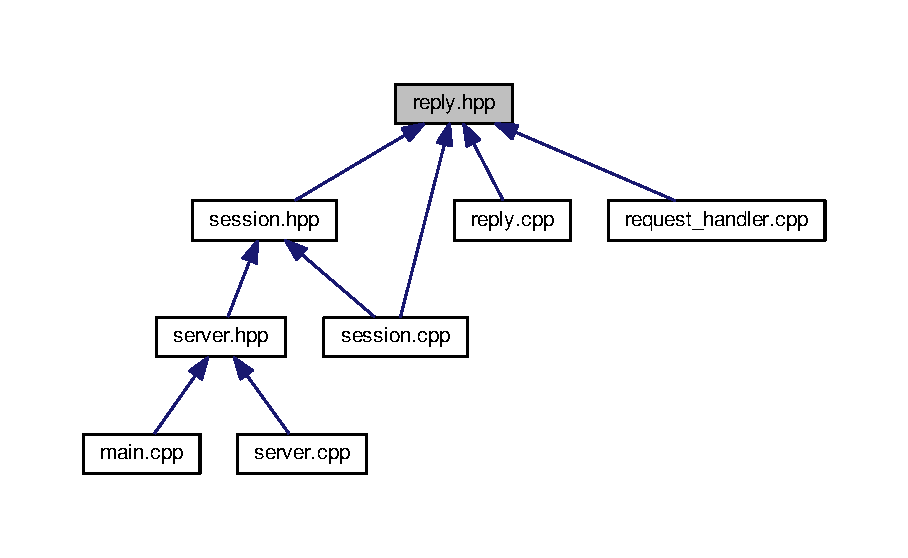
\includegraphics[width=350pt]{reply_8hpp__dep__incl}
\end{center}
\end{figure}
\subsection*{Classes}
\begin{DoxyCompactItemize}
\item 
struct \hyperlink{structwebsocket_1_1http_1_1Reply}{websocket\+::http\+::\+Reply}
\end{DoxyCompactItemize}
\subsection*{Namespaces}
\begin{DoxyCompactItemize}
\item 
 \hyperlink{namespacewebsocket}{websocket}
\item 
 \hyperlink{namespacewebsocket_1_1http}{websocket\+::http}
\end{DoxyCompactItemize}


\subsection{Detailed Description}
\begin{DoxyAuthor}{Author}
Wojciech Przybysz, Kajetan Spionek A http Reply to be sent to a client. 
\end{DoxyAuthor}

\hypertarget{request_8hpp}{}\section{request.\+hpp File Reference}
\label{request_8hpp}\index{request.\+hpp@{request.\+hpp}}
{\ttfamily \#include $<$string$>$}\\*
{\ttfamily \#include $<$vector$>$}\\*
{\ttfamily \#include \char`\"{}header.\+hpp\char`\"{}}\\*
Include dependency graph for request.\+hpp\+:\nopagebreak
\begin{figure}[H]
\begin{center}
\leavevmode
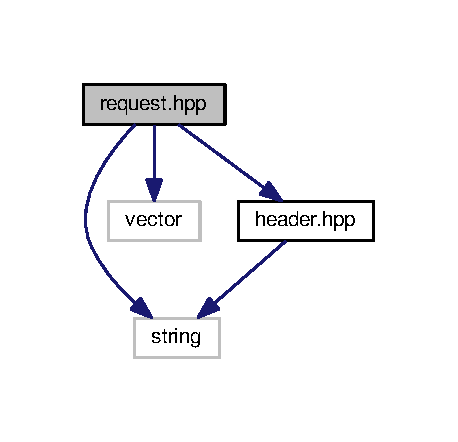
\includegraphics[width=220pt]{request_8hpp__incl}
\end{center}
\end{figure}
This graph shows which files directly or indirectly include this file\+:\nopagebreak
\begin{figure}[H]
\begin{center}
\leavevmode
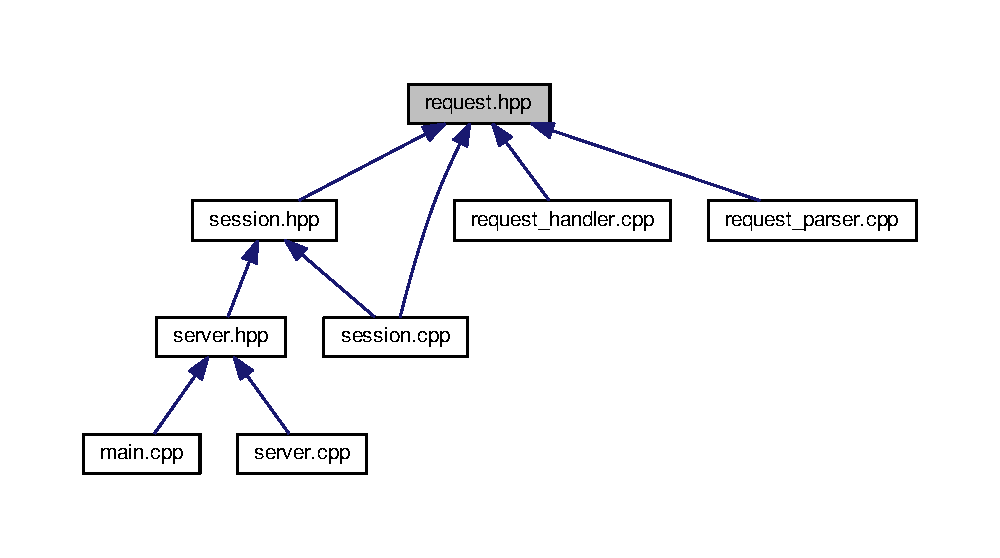
\includegraphics[width=350pt]{request_8hpp__dep__incl}
\end{center}
\end{figure}
\subsection*{Classes}
\begin{DoxyCompactItemize}
\item 
struct \hyperlink{structwebsocket_1_1http_1_1Request}{websocket\+::http\+::\+Request}
\end{DoxyCompactItemize}
\subsection*{Namespaces}
\begin{DoxyCompactItemize}
\item 
 \hyperlink{namespacewebsocket}{websocket}
\item 
 \hyperlink{namespacewebsocket_1_1http}{websocket\+::http}
\end{DoxyCompactItemize}


\subsection{Detailed Description}
\begin{DoxyAuthor}{Author}
Wojciech Przybysz, Kajetan Spionek A http request received from a client. 
\end{DoxyAuthor}

\hypertarget{request__handler_8cpp}{}\section{request\+\_\+handler.\+cpp File Reference}
\label{request__handler_8cpp}\index{request\+\_\+handler.\+cpp@{request\+\_\+handler.\+cpp}}
{\ttfamily \#include \char`\"{}request\+\_\+handler.\+hpp\char`\"{}}\\*
{\ttfamily \#include $<$sstream$>$}\\*
{\ttfamily \#include $<$boost/lexical\+\_\+cast.\+hpp$>$}\\*
{\ttfamily \#include $<$boost/uuid/sha1.\+hpp$>$}\\*
{\ttfamily \#include $<$boost/archive/iterators/base64\+\_\+from\+\_\+binary.\+hpp$>$}\\*
{\ttfamily \#include $<$boost/archive/iterators/insert\+\_\+linebreaks.\+hpp$>$}\\*
{\ttfamily \#include $<$boost/archive/iterators/transform\+\_\+width.\+hpp$>$}\\*
{\ttfamily \#include $<$boost/archive/iterators/ostream\+\_\+iterator.\+hpp$>$}\\*
{\ttfamily \#include \char`\"{}header.\+hpp\char`\"{}}\\*
{\ttfamily \#include \char`\"{}reply.\+hpp\char`\"{}}\\*
{\ttfamily \#include \char`\"{}request.\+hpp\char`\"{}}\\*
Include dependency graph for request\+\_\+handler.\+cpp\+:
\nopagebreak
\begin{figure}[H]
\begin{center}
\leavevmode
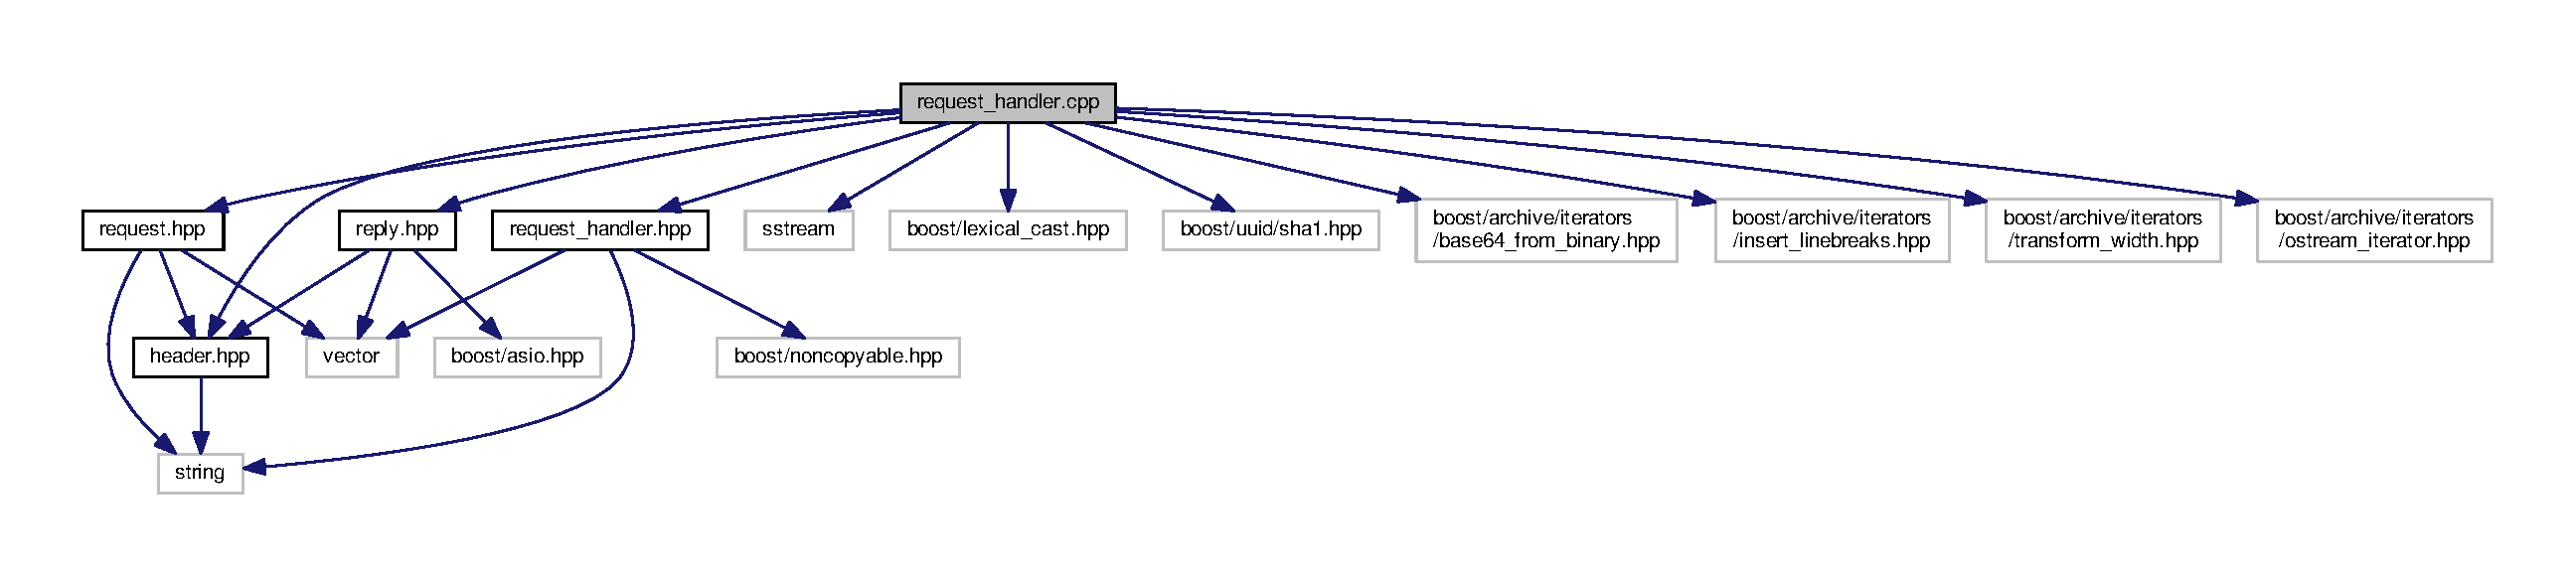
\includegraphics[width=350pt]{request__handler_8cpp__incl}
\end{center}
\end{figure}
\subsection*{Namespaces}
\begin{DoxyCompactItemize}
\item 
 \hyperlink{namespacewebsocket}{websocket}
\item 
 \hyperlink{namespacewebsocket_1_1http}{websocket\+::http}
\end{DoxyCompactItemize}

\hypertarget{request__handler_8hpp}{}\section{request\+\_\+handler.\+hpp File Reference}
\label{request__handler_8hpp}\index{request\+\_\+handler.\+hpp@{request\+\_\+handler.\+hpp}}
{\ttfamily \#include $<$string$>$}\\*
{\ttfamily \#include $<$vector$>$}\\*
{\ttfamily \#include $<$boost/noncopyable.\+hpp$>$}\\*
Include dependency graph for request\+\_\+handler.\+hpp\+:
\nopagebreak
\begin{figure}[H]
\begin{center}
\leavevmode
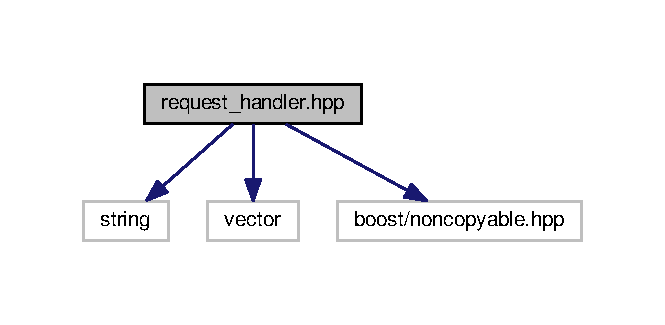
\includegraphics[width=319pt]{request__handler_8hpp__incl}
\end{center}
\end{figure}
This graph shows which files directly or indirectly include this file\+:
\nopagebreak
\begin{figure}[H]
\begin{center}
\leavevmode
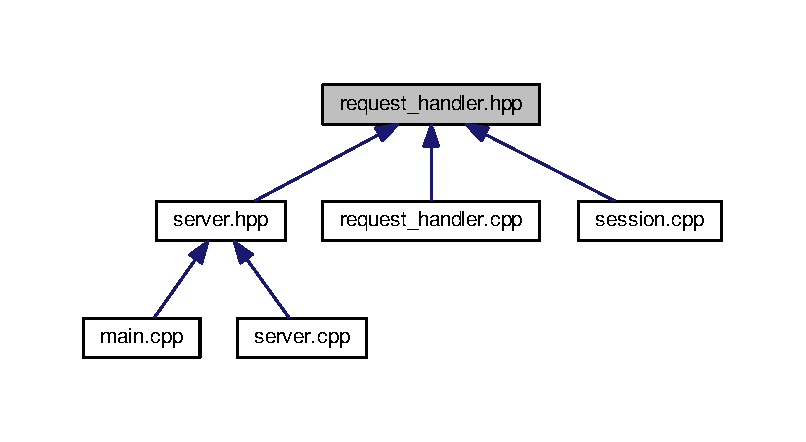
\includegraphics[width=350pt]{request__handler_8hpp__dep__incl}
\end{center}
\end{figure}
\subsection*{Classes}
\begin{DoxyCompactItemize}
\item 
class \hyperlink{classwebsocket_1_1http_1_1RequestHandler}{websocket\+::http\+::\+Request\+Handler}
\end{DoxyCompactItemize}
\subsection*{Namespaces}
\begin{DoxyCompactItemize}
\item 
 \hyperlink{namespacewebsocket}{websocket}
\item 
 \hyperlink{namespacewebsocket_1_1http}{websocket\+::http}
\end{DoxyCompactItemize}


\subsection{Detailed Description}
\begin{DoxyAuthor}{Author}
Wojciech Przybysz, Kajetan Spionek The handler for incoming http requests. 
\end{DoxyAuthor}

\hypertarget{request__parser_8cpp}{}\section{request\+\_\+parser.\+cpp File Reference}
\label{request__parser_8cpp}\index{request\+\_\+parser.\+cpp@{request\+\_\+parser.\+cpp}}
{\ttfamily \#include \char`\"{}request\+\_\+parser.\+hpp\char`\"{}}\\*
{\ttfamily \#include \char`\"{}request.\+hpp\char`\"{}}\\*
Include dependency graph for request\+\_\+parser.\+cpp\+:\nopagebreak
\begin{figure}[H]
\begin{center}
\leavevmode
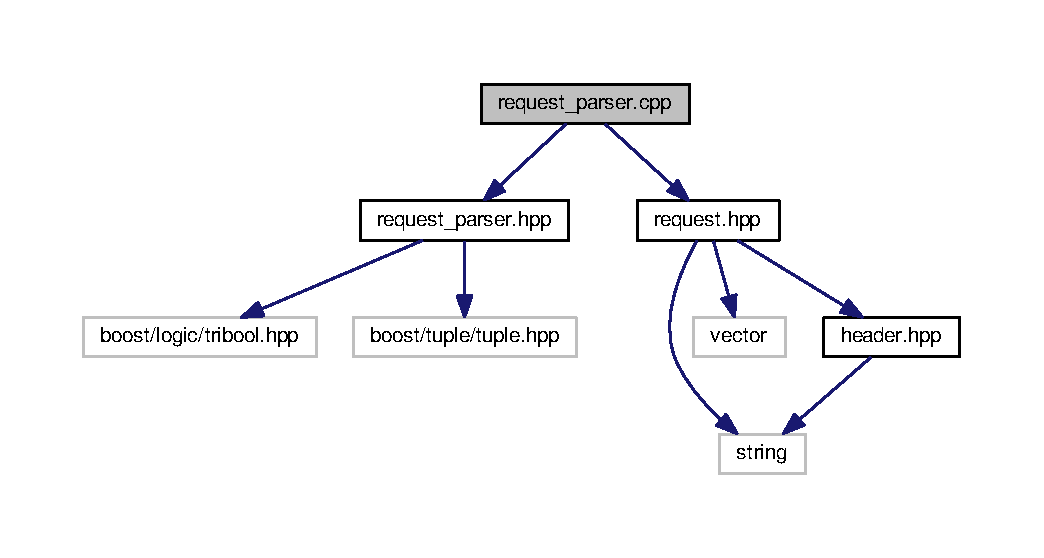
\includegraphics[width=350pt]{request__parser_8cpp__incl}
\end{center}
\end{figure}
\subsection*{Namespaces}
\begin{DoxyCompactItemize}
\item 
 \hyperlink{namespacewebsocket}{websocket}
\item 
 \hyperlink{namespacewebsocket_1_1http}{websocket\+::http}
\end{DoxyCompactItemize}

\hypertarget{request__parser_8hpp}{}\section{request\+\_\+parser.\+hpp File Reference}
\label{request__parser_8hpp}\index{request\+\_\+parser.\+hpp@{request\+\_\+parser.\+hpp}}
{\ttfamily \#include $<$boost/logic/tribool.\+hpp$>$}\\*
{\ttfamily \#include $<$boost/tuple/tuple.\+hpp$>$}\\*
Include dependency graph for request\+\_\+parser.\+hpp\+:
\nopagebreak
\begin{figure}[H]
\begin{center}
\leavevmode
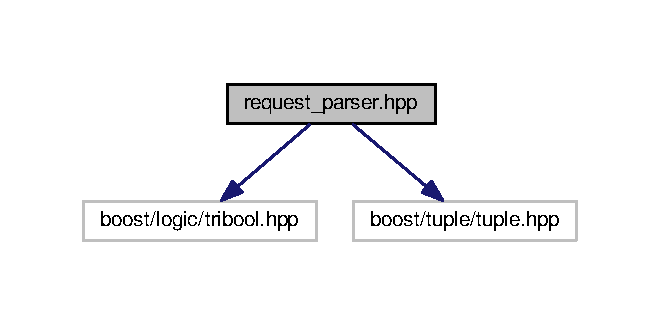
\includegraphics[width=317pt]{request__parser_8hpp__incl}
\end{center}
\end{figure}
This graph shows which files directly or indirectly include this file\+:
\nopagebreak
\begin{figure}[H]
\begin{center}
\leavevmode
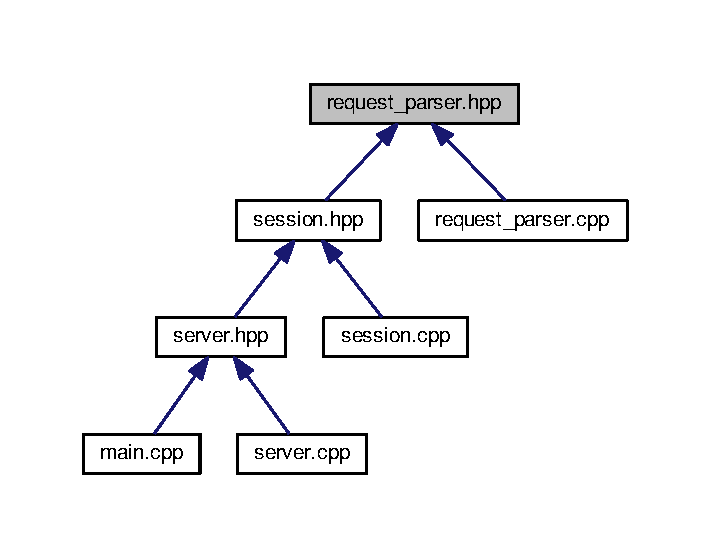
\includegraphics[width=341pt]{request__parser_8hpp__dep__incl}
\end{center}
\end{figure}
\subsection*{Classes}
\begin{DoxyCompactItemize}
\item 
class \hyperlink{classwebsocket_1_1http_1_1RequestParser}{websocket\+::http\+::\+Request\+Parser}
\end{DoxyCompactItemize}
\subsection*{Namespaces}
\begin{DoxyCompactItemize}
\item 
 \hyperlink{namespacewebsocket}{websocket}
\item 
 \hyperlink{namespacewebsocket_1_1http}{websocket\+::http}
\end{DoxyCompactItemize}


\subsection{Detailed Description}
\begin{DoxyAuthor}{Author}
Wojciech Przybysz, Kajetan Spionek Parser for incoming requests. 
\end{DoxyAuthor}

\hypertarget{server_8cpp}{}\section{server.\+cpp File Reference}
\label{server_8cpp}\index{server.\+cpp@{server.\+cpp}}
{\ttfamily \#include \char`\"{}server.\+hpp\char`\"{}}\\*
{\ttfamily \#include $<$iostream$>$}\\*
{\ttfamily \#include $<$vector$>$}\\*
{\ttfamily \#include $<$boost/bind.\+hpp$>$}\\*
{\ttfamily \#include $<$boost/shared\+\_\+ptr.\+hpp$>$}\\*
Include dependency graph for server.\+cpp\+:
\nopagebreak
\begin{figure}[H]
\begin{center}
\leavevmode
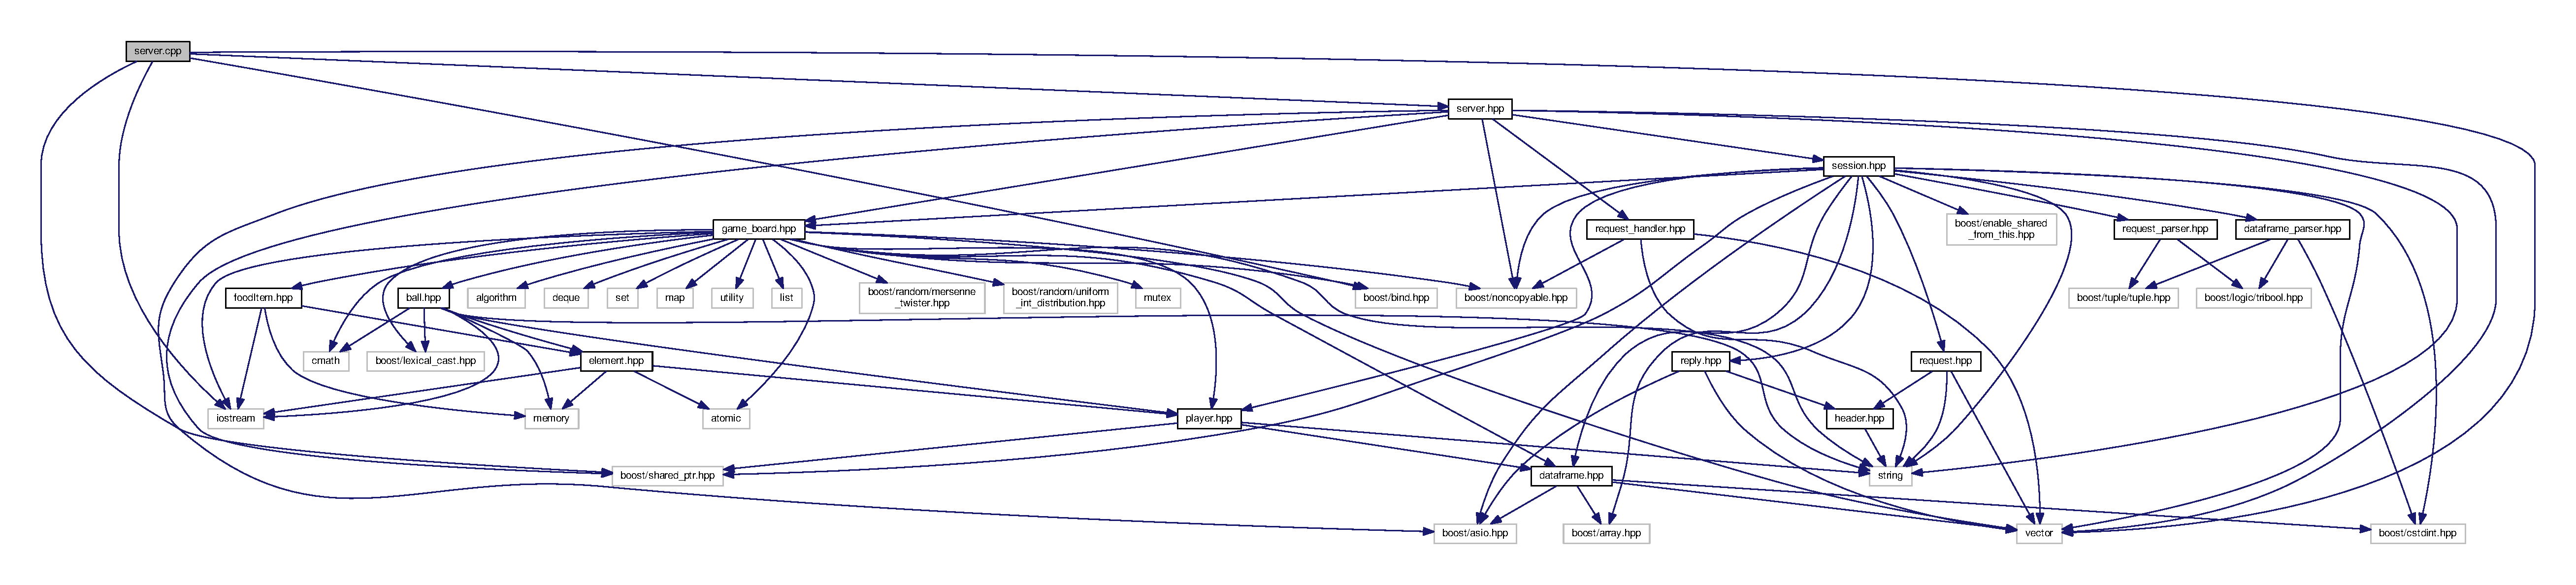
\includegraphics[width=350pt]{server_8cpp__incl}
\end{center}
\end{figure}
\subsection*{Namespaces}
\begin{DoxyCompactItemize}
\item 
 \hyperlink{namespacewebsocket}{websocket}
\end{DoxyCompactItemize}

\hypertarget{server_8hpp}{}\section{server.\+hpp File Reference}
\label{server_8hpp}\index{server.\+hpp@{server.\+hpp}}
{\ttfamily \#include $<$string$>$}\\*
{\ttfamily \#include $<$vector$>$}\\*
{\ttfamily \#include $<$boost/asio.\+hpp$>$}\\*
{\ttfamily \#include $<$boost/noncopyable.\+hpp$>$}\\*
{\ttfamily \#include $<$boost/shared\+\_\+ptr.\+hpp$>$}\\*
{\ttfamily \#include \char`\"{}game\+\_\+board.\+hpp\char`\"{}}\\*
{\ttfamily \#include \char`\"{}session.\+hpp\char`\"{}}\\*
{\ttfamily \#include \char`\"{}request\+\_\+handler.\+hpp\char`\"{}}\\*
Include dependency graph for server.\+hpp\+:
\nopagebreak
\begin{figure}[H]
\begin{center}
\leavevmode
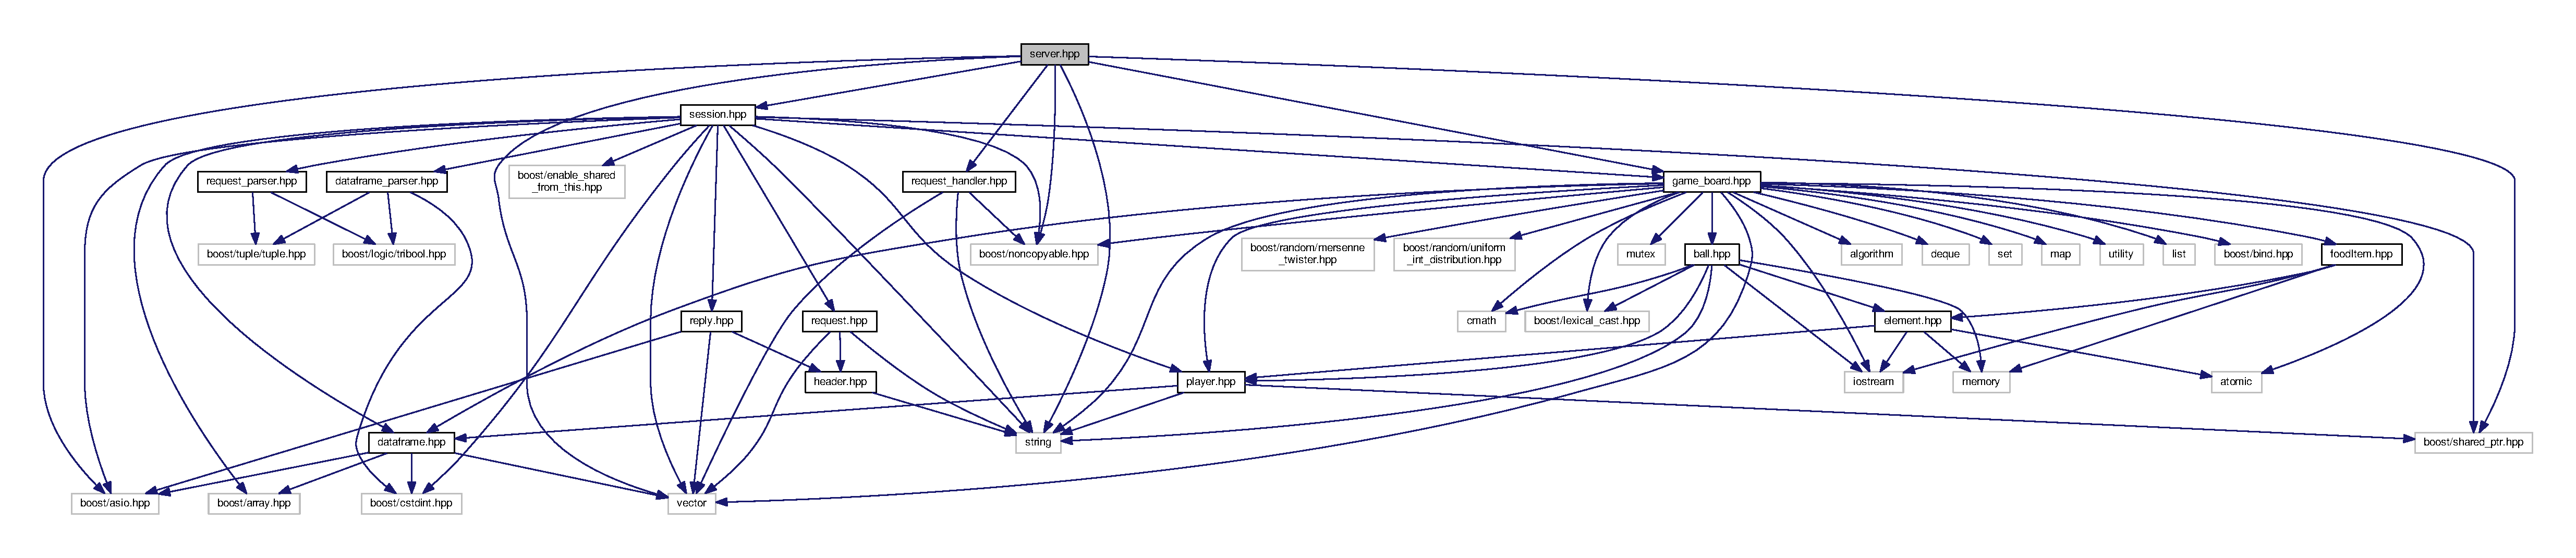
\includegraphics[width=350pt]{server_8hpp__incl}
\end{center}
\end{figure}
This graph shows which files directly or indirectly include this file\+:\nopagebreak
\begin{figure}[H]
\begin{center}
\leavevmode
\includegraphics[width=216pt]{server_8hpp__dep__incl}
\end{center}
\end{figure}
\subsection*{Classes}
\begin{DoxyCompactItemize}
\item 
class \hyperlink{classwebsocket_1_1Server}{websocket\+::\+Server}
\end{DoxyCompactItemize}
\subsection*{Namespaces}
\begin{DoxyCompactItemize}
\item 
 \hyperlink{namespacewebsocket}{websocket}
\end{DoxyCompactItemize}


\subsection{Detailed Description}
\begin{DoxyAuthor}{Author}
Wojciech Przybysz, Kajetan Spionek /// The top-\/level class of the server. 
\end{DoxyAuthor}

\hypertarget{session_8cpp}{}\section{session.\+cpp File Reference}
\label{session_8cpp}\index{session.\+cpp@{session.\+cpp}}
{\ttfamily \#include \char`\"{}session.\+hpp\char`\"{}}\\*
{\ttfamily \#include \char`\"{}reply.\+hpp\char`\"{}}\\*
{\ttfamily \#include \char`\"{}request.\+hpp\char`\"{}}\\*
{\ttfamily \#include \char`\"{}request\+\_\+handler.\+hpp\char`\"{}}\\*
{\ttfamily \#include $<$iostream$>$}\\*
{\ttfamily \#include $<$vector$>$}\\*
{\ttfamily \#include $<$boost/lexical\+\_\+cast.\+hpp$>$}\\*
{\ttfamily \#include $<$boost/bind.\+hpp$>$}\\*
{\ttfamily \#include $<$boost/uuid/sha1.\+hpp$>$}\\*
{\ttfamily \#include $<$boost/archive/iterators/base64\+\_\+from\+\_\+binary.\+hpp$>$}\\*
{\ttfamily \#include $<$boost/archive/iterators/insert\+\_\+linebreaks.\+hpp$>$}\\*
{\ttfamily \#include $<$boost/archive/iterators/transform\+\_\+width.\+hpp$>$}\\*
{\ttfamily \#include $<$boost/archive/iterators/ostream\+\_\+iterator.\+hpp$>$}\\*
Include dependency graph for session.\+cpp\+:
\nopagebreak
\begin{figure}[H]
\begin{center}
\leavevmode
\includegraphics[width=350pt]{session_8cpp__incl}
\end{center}
\end{figure}
\subsection*{Namespaces}
\begin{DoxyCompactItemize}
\item 
 \hyperlink{namespacewebsocket}{websocket}
\end{DoxyCompactItemize}

\hypertarget{session_8hpp}{}\section{session.\+hpp File Reference}
\label{session_8hpp}\index{session.\+hpp@{session.\+hpp}}
{\ttfamily \#include $<$string$>$}\\*
{\ttfamily \#include $<$vector$>$}\\*
{\ttfamily \#include $<$boost/cstdint.\+hpp$>$}\\*
{\ttfamily \#include $<$boost/asio.\+hpp$>$}\\*
{\ttfamily \#include $<$boost/array.\+hpp$>$}\\*
{\ttfamily \#include $<$boost/noncopyable.\+hpp$>$}\\*
{\ttfamily \#include $<$boost/shared\+\_\+ptr.\+hpp$>$}\\*
{\ttfamily \#include $<$boost/enable\+\_\+shared\+\_\+from\+\_\+this.\+hpp$>$}\\*
{\ttfamily \#include \char`\"{}reply.\+hpp\char`\"{}}\\*
{\ttfamily \#include \char`\"{}request.\+hpp\char`\"{}}\\*
{\ttfamily \#include \char`\"{}request\+\_\+parser.\+hpp\char`\"{}}\\*
{\ttfamily \#include \char`\"{}dataframe.\+hpp\char`\"{}}\\*
{\ttfamily \#include \char`\"{}dataframe\+\_\+parser.\+hpp\char`\"{}}\\*
{\ttfamily \#include \char`\"{}player.\+hpp\char`\"{}}\\*
{\ttfamily \#include \char`\"{}game\+\_\+board.\+hpp\char`\"{}}\\*
Include dependency graph for session.\+hpp\+:
\nopagebreak
\begin{figure}[H]
\begin{center}
\leavevmode
\includegraphics[width=350pt]{session_8hpp__incl}
\end{center}
\end{figure}
This graph shows which files directly or indirectly include this file\+:
\nopagebreak
\begin{figure}[H]
\begin{center}
\leavevmode
\includegraphics[width=265pt]{session_8hpp__dep__incl}
\end{center}
\end{figure}
\subsection*{Classes}
\begin{DoxyCompactItemize}
\item 
class \hyperlink{classwebsocket_1_1Session}{websocket\+::\+Session}
\end{DoxyCompactItemize}
\subsection*{Namespaces}
\begin{DoxyCompactItemize}
\item 
 \hyperlink{namespacewebsocket}{websocket}
\end{DoxyCompactItemize}
\subsection*{Typedefs}
\begin{DoxyCompactItemize}
\item 
typedef boost\+::shared\+\_\+ptr$<$ Session $>$ \hyperlink{namespacewebsocket_a12d8500a66e77dc9bfbff046b86714d8}{websocket\+::session\+\_\+ptr}
\end{DoxyCompactItemize}


\subsection{Detailed Description}
\begin{DoxyAuthor}{Author}
Wojciech Przybysz, Kajetan Spionek Represents a single connection from a client. 
\end{DoxyAuthor}

%--- End generated contents ---

% Index
\backmatter
\newpage
\phantomsection
\clearemptydoublepage
\addcontentsline{toc}{chapter}{Index}
\printindex

\end{document}
